\documentclass[12pt, twocolumn]{article}
\usepackage[margin=3cm]{geometry}
\usepackage{listings}
\usepackage{graphicx}
\renewcommand{\lstlistingname}{\textbf{Program}}
\graphicspath{Lab1}


\begin{document}

\begin{titlepage}
	\begin{center}
		
		
		% Upper part of the page. The '~' is needed because \\
		% only works if a paragraph has started.
		\vfill
		
		\textsc{\LARGE Experiment 1: Introduction to the Sanper-1 Educational \\ Lab Unit}\\[1.5cm]
		
		\Large Adam Sumner\\[0.5cm]
		
		\Large Illinois Insititute of Technology\\[0.5cm]
		
		\Large ECE 441-01\\[0.5cm]	
		% Author and supervisor
		\noindent
		\vfill
		\large \textbf{Lab Date:} January 20th, 2015\hfill
		\large \textbf{Due Date:} January 27th, 2015
		% Bottom of the page
		
		
	\end{center}
\end{titlepage}

\section{Introduction}
The purpose of this lab is to introduce the student to the \textsc{SANPER-1 Educational Lab Unit}, the \textsc{TUTOR} command set, the \textsc{TUTOR} Trap \#14 Handler, and the MC68000 Instruction set. It is intended to promote familiarity with the basic commands offered by \textsc{TUTOR}, as well as the manner in which \textsc{TUTOR} operates. The student is instructed to practice useful \textsc{TUTOR} commands as well as load several basic programs into the \textsc{ELU} and then step through each program.
\section{Background}
The \textsc{SANPER-1 Educational Lab Unit} was designed and developed by Dr. Jafar Saniie and Mr. Stephen Perich. The \textsc{ELU} utilizes the Motorola MC68000, which is a 16-bit microprocessor whose external address and data buses are 23 and 16 lines wide respectively. This unit is also equipped with a firmware package named \textsc{TUTOR} which is a MC68K monitor program\cite{sanper}. The \textsc{SANPER-1 ELU} consists of the following components:
\begin{itemize}
	\item System Board
	\item Display Board
	\item System Expansion Board
	\item 150 Watt IBM PC/XT compatible power supply
	\item IBM PC compatible chassis
	\item MC68000 Microprocessor
	\item 208k bytes of static RAM
	\item 32k bytes of EPROM
	\item 3 serial ports
	\item 2 parallel ports
	\item A/D converter
	\item D/A converter
	\item Speech Synthesizer
	\item 2 high power output drives
	\item Internal cabling
\end{itemize}
The \textsc{ELU} is also equipped with some special features. One feature explored in this lab is called the Single-Step Hardware Mode. The single step circuitry allows the user to observe every bus cycle of the MC68K in a static state\cite{sanper}. In this mode, the MC68K's address, data, and control signals are frozen in time and are displayed on the front display board. Using the \textsc{SINGLE STEP PULSE} button, the user is able to advance to the next bus cycle. This feature is primarily used to observe the intermediate steps that occur during the execution of a single MC68K instruction.

The \textsc{TUTOR} resident monitor is the environment in which the user can perform programming and debugging work on the \textsc{SANPER-1 ELU}. It is command line based and provides several helpful commands to the user such as:

\begin{itemize}
	\item \textbf{MD} (Memory Display)
	\item \textbf{MM} (Memory Modify)
	\item \textbf{MS} (Memory Set)
	\item \textbf{.A0 - .A7} (Display/Set Address Register)
	\item \textbf{.D0 - .D7} (Display/Set Data Register)
	\item \textbf{.PC} (Display/Set Program Counter)
	\item \textbf{.SR} (Display/Set Status Register)
	\item \textbf{DF} (Display Formatted Registers)
	\item \textbf{Go, G} (Go)
	\item \textbf{TR, T} (Trace)
	
\end{itemize} 
One of the most critical functions of \textsc{TUTOR} is the TRAP 14 handler. This is a command that can be called to execute system calls from the user level. This allows the user to utilize important features such as I/O\cite{ecbm}.
\section{Equipment/Procedure}
\subsection{Equipment}
\begin{itemize}
	\item \textsc{SANPER-1 Educational Lab Unit}
	\item Computer with TUTOR software
\end{itemize}
\subsection{Procedure}
\subsubsection{Part A}
\begin{enumerate}
	\item Turn on \textsc{SANPER-1 ELU} and connected computer
	\item Type in the \textbf{HE} command
	\item Type in the \textbf{DF} command
	\item Modify the Status Register to 0000
	\item Examine Status Register using the \textbf{DF} command
	\item Modify the Status Register to FFFF
	\item Examine Status Register using the \textbf{DF} command
	\item Modify Address Register A1 to 1234
	\item Examine the A1 register using the \textbf{.A1} command
	\item Display all address registers using the \textbf{.A} command
	\item Display all data registers using the \textbf{.D} command
\end{enumerate}
\subsubsection{Part B}
\begin{enumerate}
	\item Type Program from Section \ref{prog1} into the lab unit using the \textbf{MM} command
	\item Type \textbf{MS} \$900 'IT WORKS !!'
	\item Run program using the \textbf{G} command
	\item Press \textsc{ABORT} button to exit
	\item Trace through program using the \textbf{T} command
	\item Type the programs listed in Sections \ref{prog2}-\ref{prog4} and step through each using the hardware single-step mode.
	\item Place the \textsc{SANPER-1 ELU} in hardware single-step mode, press reset, and step through eight times
\end{enumerate}
\section{Results}
The results obtained are all included in the Appendix in Section \ref{appendix}. The step through data collected for each program is shown in Sections \ref{progpic1}-\ref{progpic4}. The reset step through data is shown in Section \ref{resetpic}. The data obtained from the software abort during the execution of \textbf{Program 1} from Section \ref{prog1} is shown in Section \ref{abort}.
\section{Discussion}
\subsection{Answers to Follow Up Questions}
\begin{enumerate}
	\item Completed listing of all the program segments. Your listings must include meaningful global and local comments
	\subitem \hspace{-0.7cm}\textbf{Answer:} Programs are located in the Appendix in Sections \ref{prog1}-\ref{prog4}
	\item What is the address range of the available memory within the \textsc{SANPER-1 ELU} that may be used for your program? Describe your answer
	\subitem \hspace{-0.7cm}\textbf{Answer:} According to the \textsc{SANPER-1} User Manual, User Memory is located at memory addresses \$000900-\$003FFF. Addresses \$004000-\$007FFF are unused, unlike Motorola's Educational Board which uses address range \$000900-\$007FFF for user memory.
	\item List the value of the address, data, and control lines during the hardware step-through of each program, and discuss any unusual events that may have occured
	\subitem \hspace{-0.7cm}\textbf{Answer:} The values can be found in the photos shown in the Appendix in Sections \ref{progpic1}-\ref{progpic4}. Generally, the address line increased by the word size of the MC68K, due to the execution of each instruction. However, when data needed to be fetched from or written to memory, the address line changed to the specified address. The data line contained either the instruction to be fetched next or the data to be stored/loaded. When the TRAP \#14 handler was called, the address line changed to its appropriate address. 
	\item How many serial ports are available on a \textsc{SANPER-1 ELU}? What are the specific memory addresses associated with these ports?
	\subitem \hspace{-0.7cm}\textbf{Answer:} There are three serial ports. Port 1 which is usually connected to the terminal, Port 2 which provides a link to a host computer, and Port 3 which is for general purpose. Port 1(ACIA1) is associated with even addresses \$010040 and \$010042 while Port 2(ACIA2) is associated with odd addresses \$010041 and \$010043. Port 3(ACIA3) is associated with addresses \$010044-\$010046. 
	\item List all the possible ways to interface your hardware design to the \textsc{SANPER-1 ELU}
	\subitem \hspace{-0.7cm}\textbf{Answer:} You can interface your hardware design using the \textsc{SANPER-1}'s serial ports, parallel ports, A/D Converter, D/A converter, speech synthesizer, and its high power output drives.
	\item When the MC68K control signals "*AS", "*UDS", or "*LDS", are asserted, what is the status of the respective LED (on or off), and why?
	\subitem \hspace{-0.7cm}\textbf{Answer:} The LED is off. Those signals assert at low voltage levels.
\end{enumerate}
\subsection{Analysis}
Because this experiment is designed to be an introductory tutorial for the student, there is little to discuss on the results obtained. However, the skills learned during this experiment should be noted and kept in the students arsenal of tools for use in future experiments.  
\section{Conclusion}
Overall, the experiment was a success. The \textsc{SANPER-1 ELU} and \textsc{TUTOR} were both introduced to the student, as well as the TRAP \#14 handler. From here, the student should prepare for future experiments that utilize the basic concepts learned in this experiment.
\onecolumn
\section{Appendix}
\label{appendix}
\subsection{Code}
\subsubsection{Program 1: \normalfont IT WORKS !! Loop}
\label{prog1}
\lstset{language=[Motorola68K]Assembler}
\begin{lstlisting}
LEA.L	$2000,A7	;Load memory address
MOVE.L	#$900,A5	;Prepare registers
MOVE.L	#$90B,A6	
MOVE.B	#243,D7		;Set syscall to output to port 1
TRAP 	#14
MOVE.B	#241,D7		;Set syscall to input string from port 1
TRAP	#14
MOVE.B	#227,D7		;Set syscall to output string with newline to 
			;port 1
TRAP	#14
BRA	$1004		;Loop back to preparing the registers
\end{lstlisting}

\subsubsection{Program 2: \normalfont First Infinite Data Transfer Loop}
\label{prog2}
\begin{lstlisting}
MOVE.B	D0,D1		;Move contents of data register 0 to data 
			;register 1
MOVE.B	#$AA,$1000	;Move constant to memory address
BRA	$900		;Loop back to first instruction
\end{lstlisting}

\subsubsection{Program 3: \normalfont Second Infinite Data Transfer Loop}
\label{prog3}
\begin{lstlisting}
MOVE.B	D0,D1		;Move contents of data register 0 to data 
			;register 1
MOVE.B	#$AA,$1001	;Move constant to memory address
BRA	$900		;Loop back to first instruction
\end{lstlisting}

\subsubsection{Program 4: \normalfont Third Infinite Data Transfer Loop}
\label{prog4}
\begin{lstlisting}
MOVE.B	D0,D1		;Move contents of data register 0 to data 
			;register 1
MOVE.B	$1000,$1001	;Move value from memory address to memory address
BRA	$900		;Loop back to first instruction
\end{lstlisting}

\subsection{Step Through Program Data}
\twocolumn
\subsubsection{Program 1}
\label{progpic1}
\begin{center}
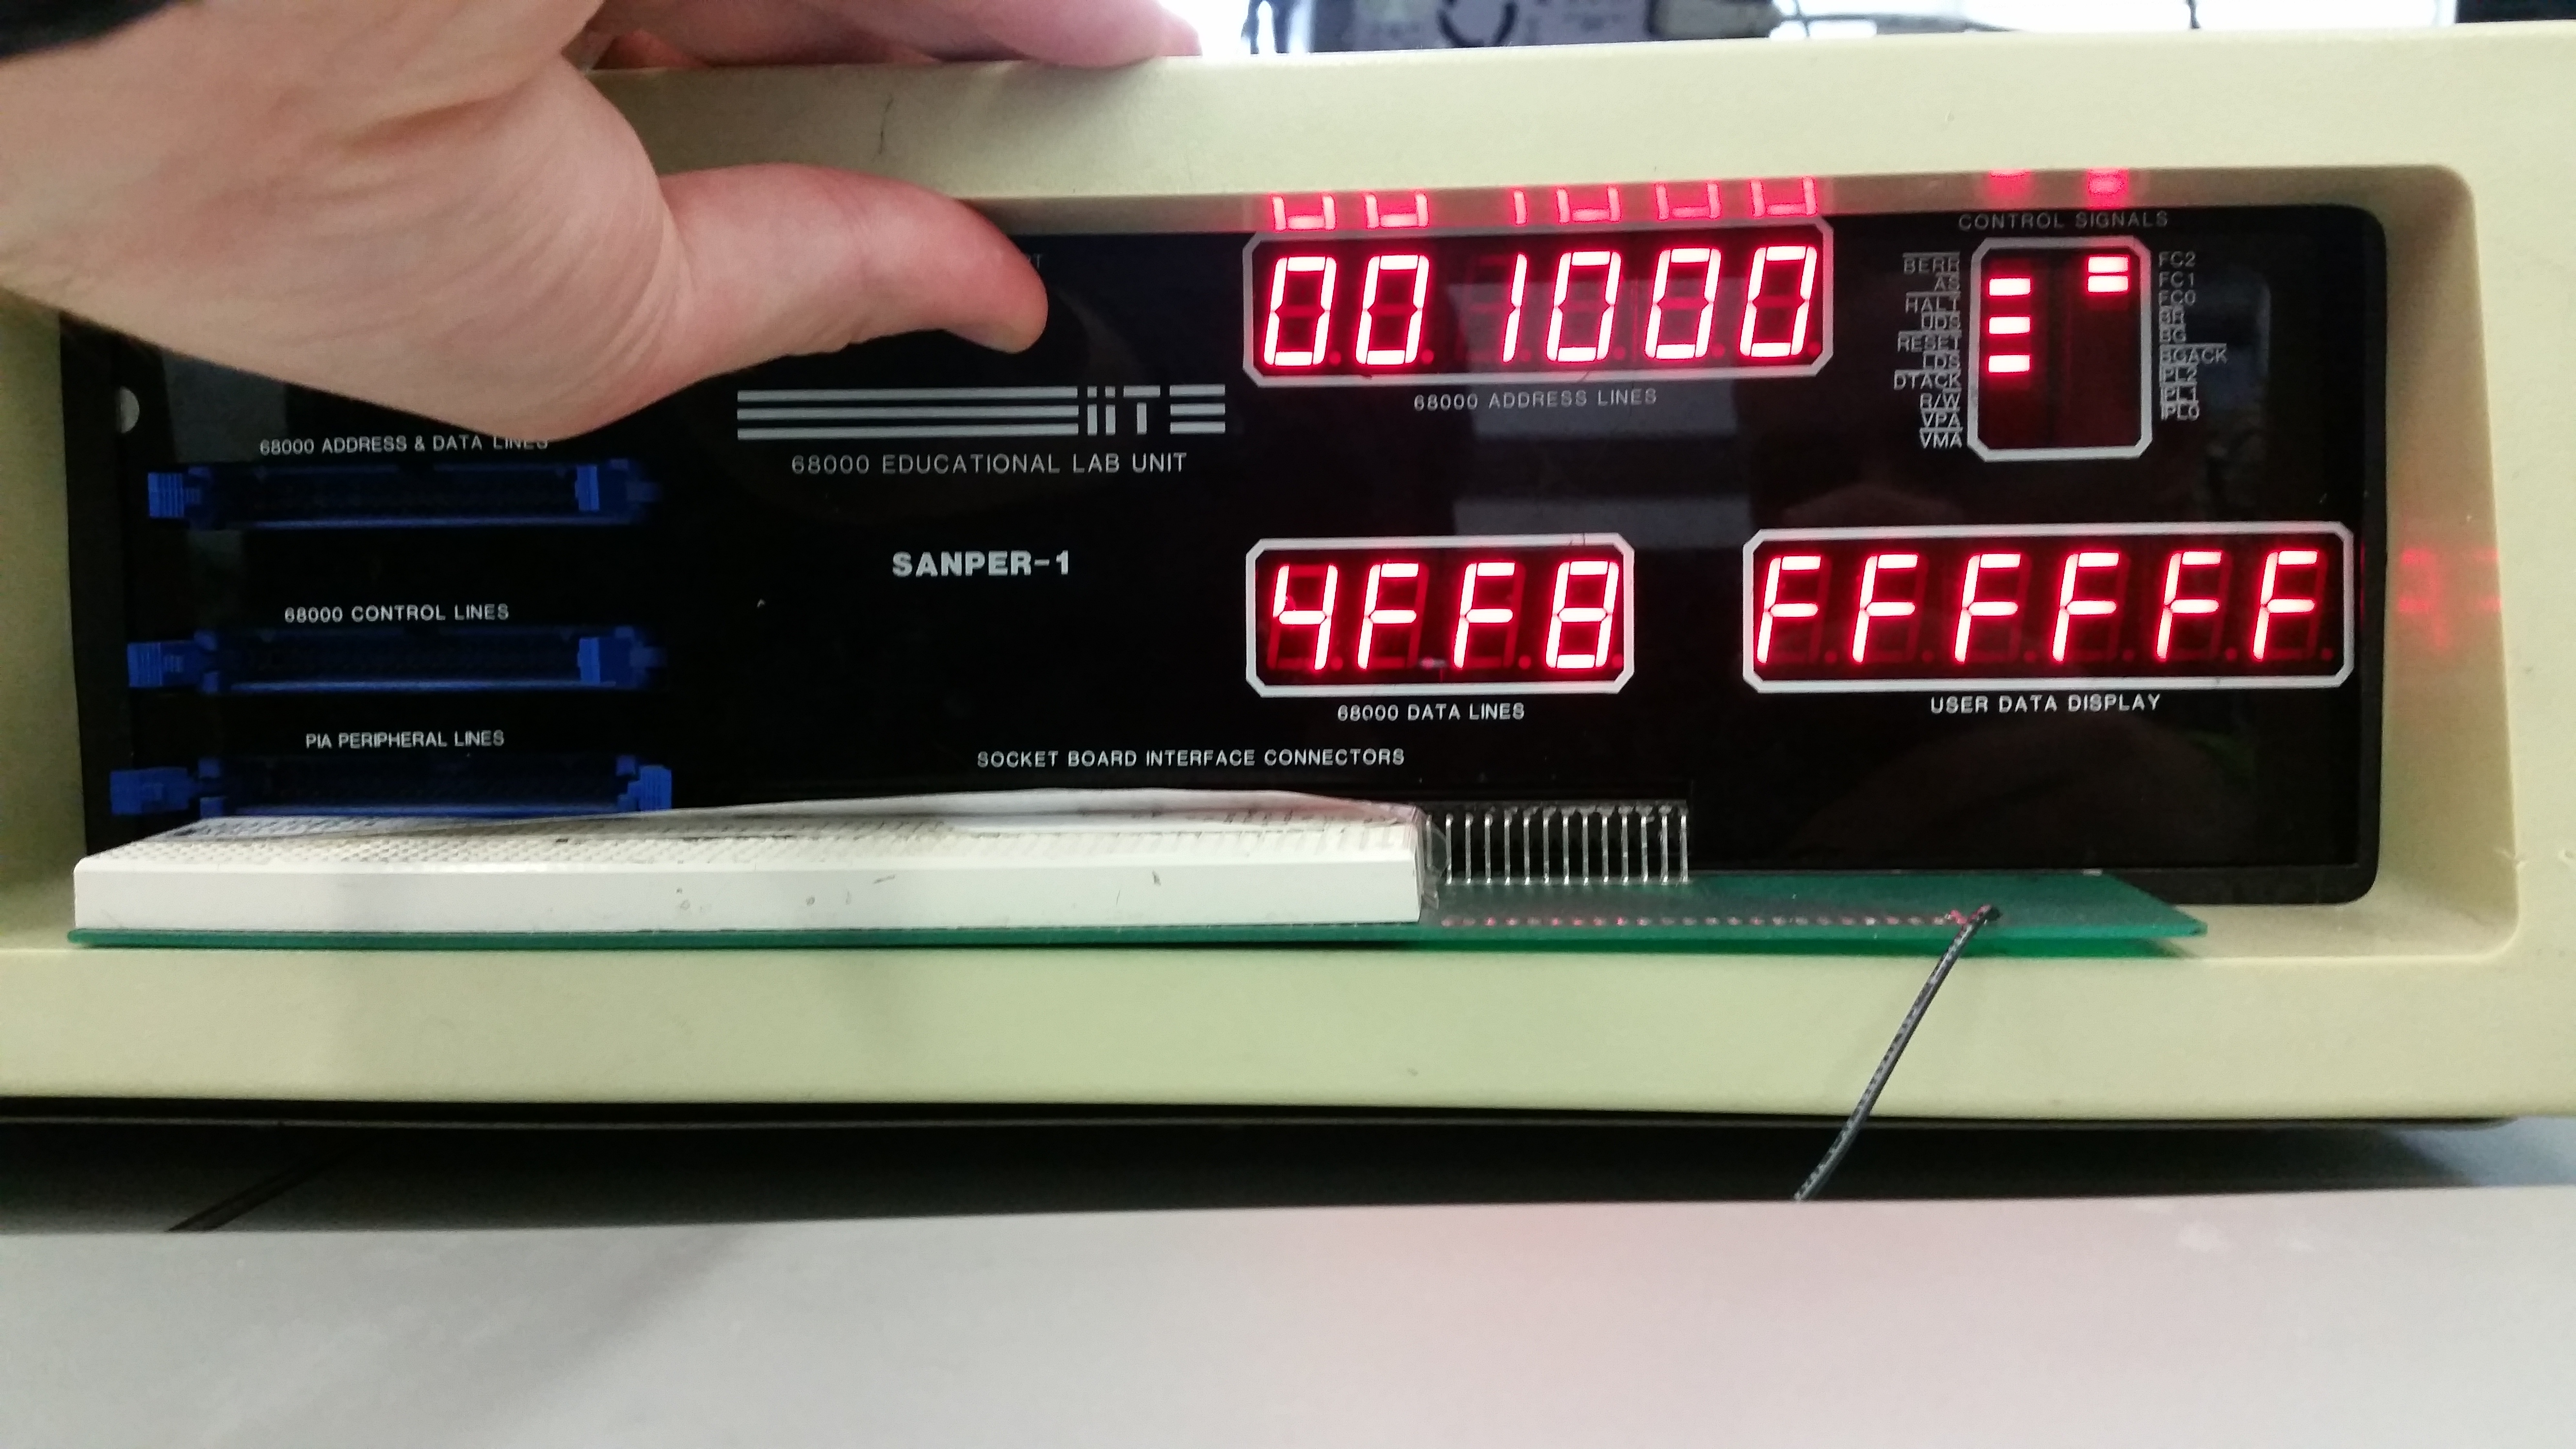
\includegraphics[width=\linewidth]{Lab1/20150120_093554}
\end{center}code
\begin{center}
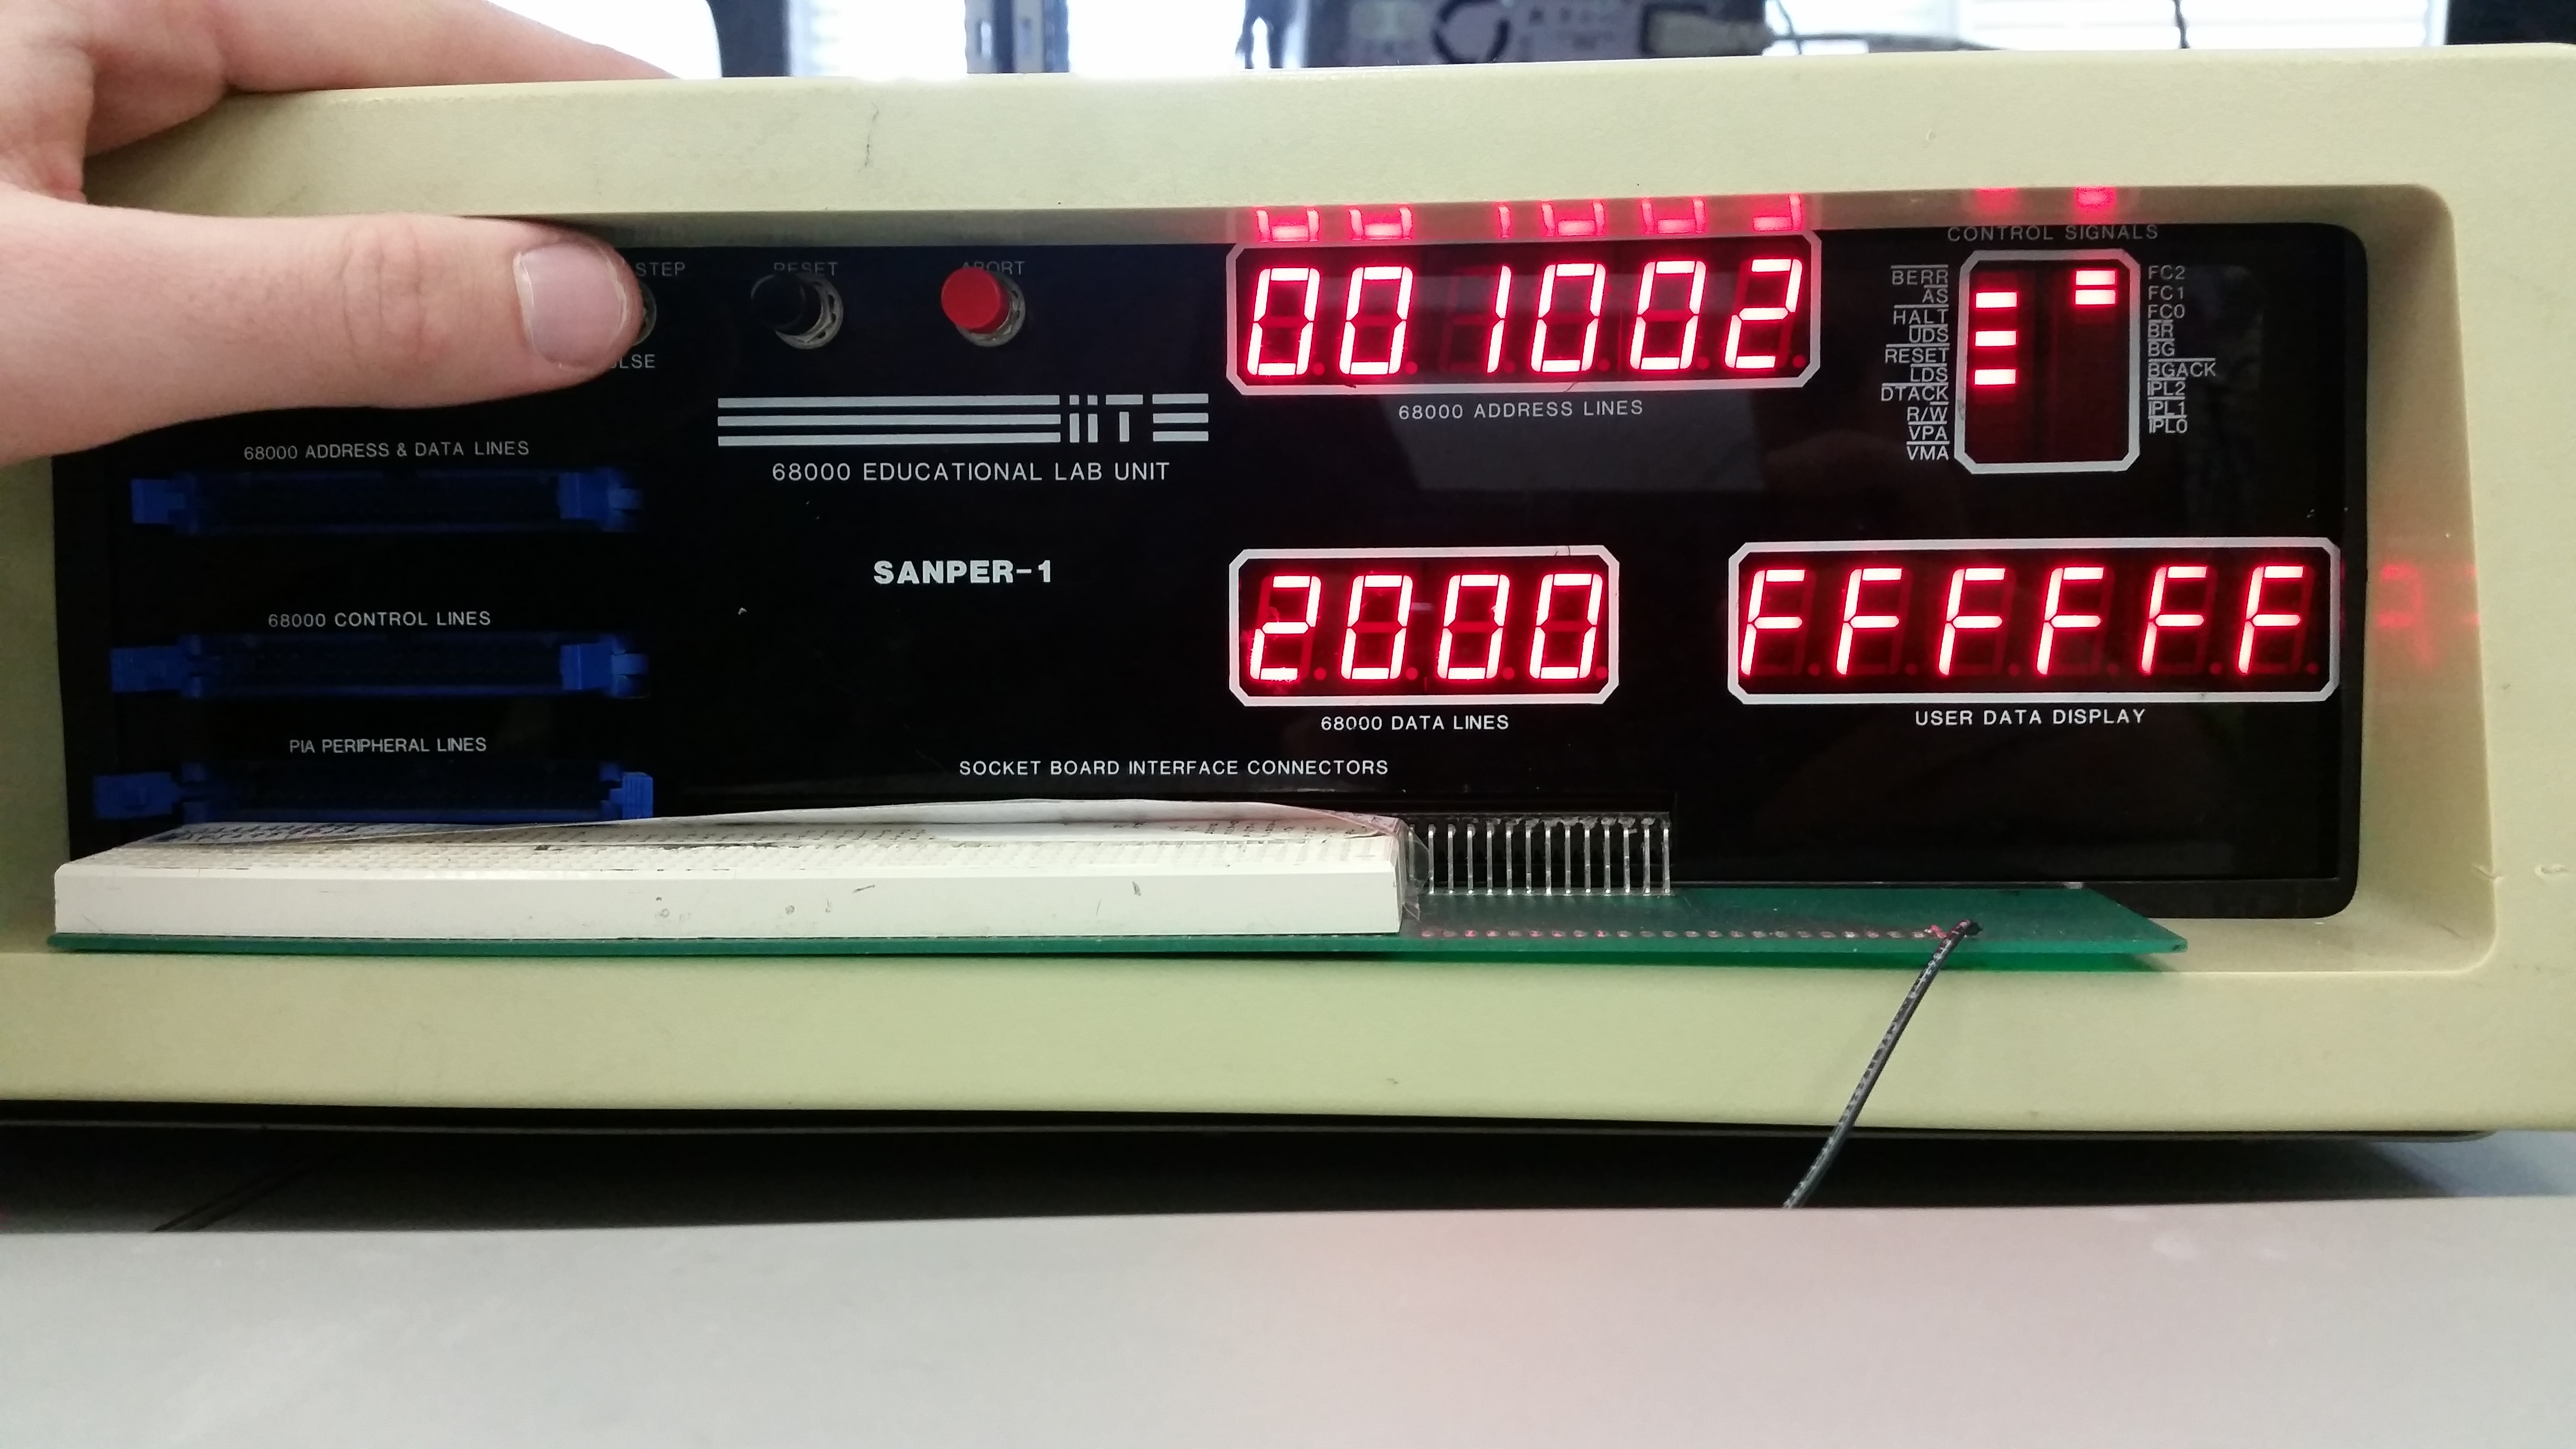
\includegraphics[width=\linewidth]{Lab1/20150120_093559}
\end{center}
\begin{center}
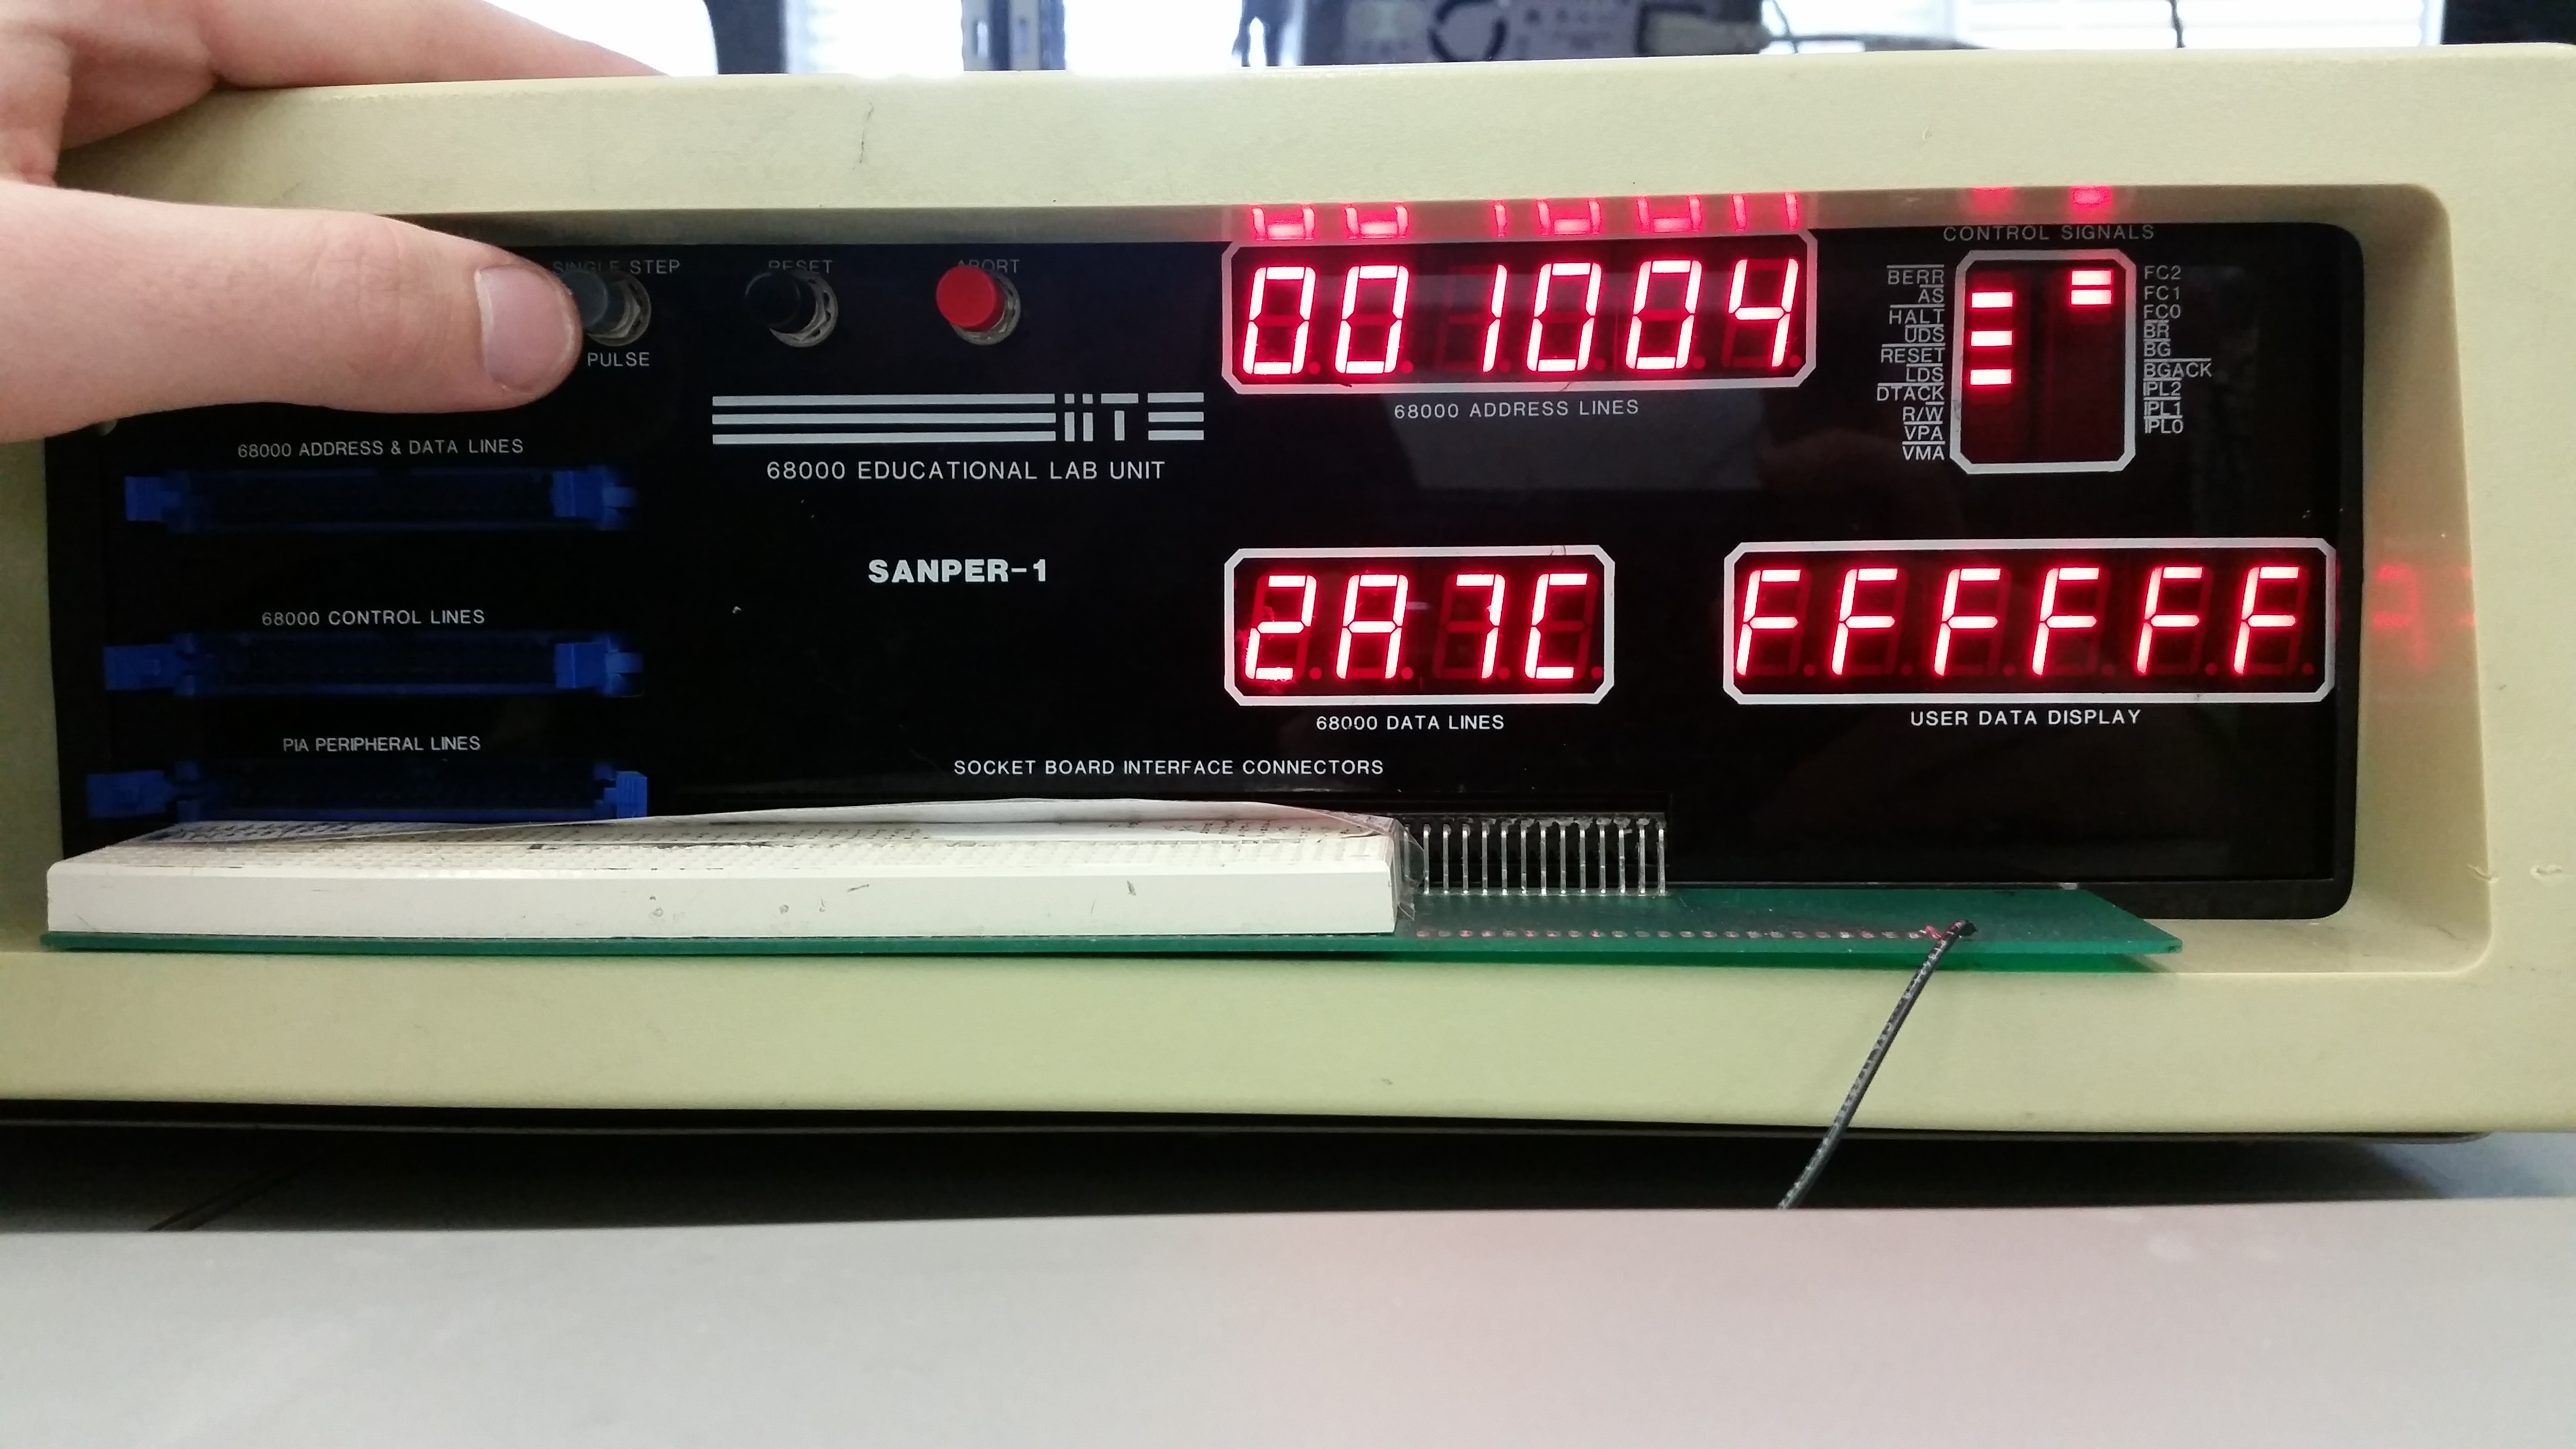
\includegraphics[width=\linewidth]{Lab1/20150120_093601}
\end{center}
\begin{center}
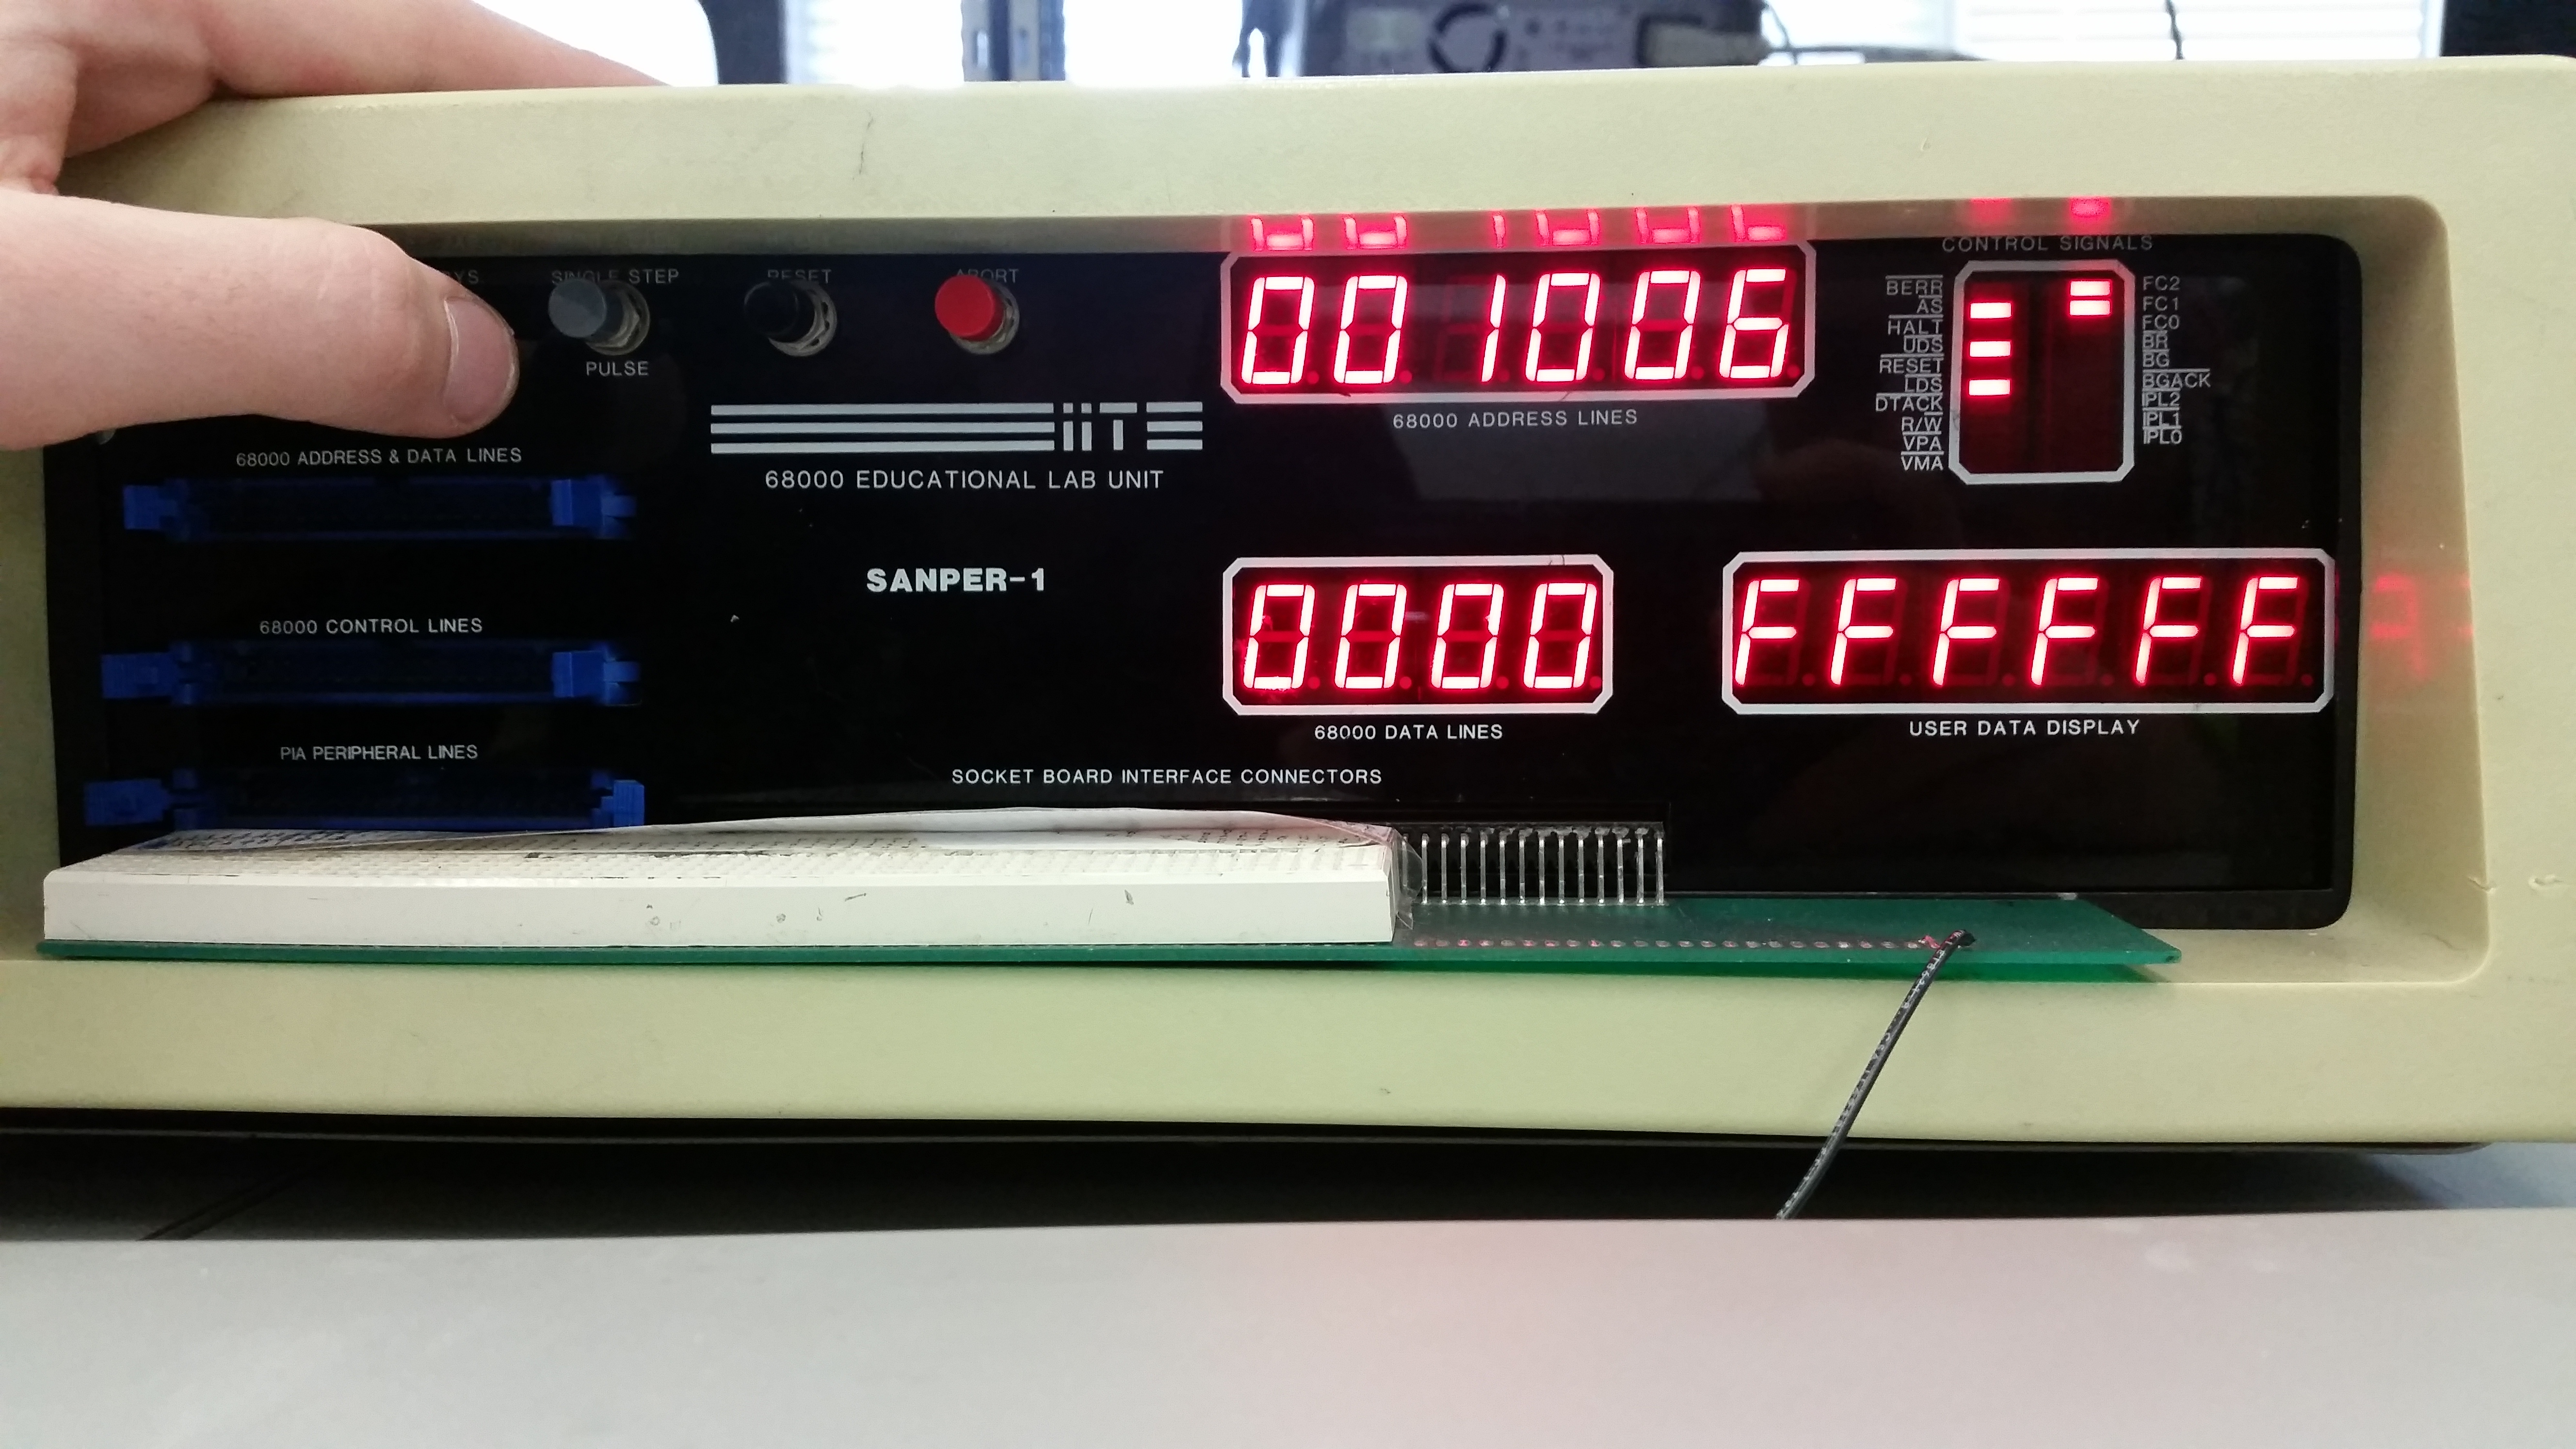
\includegraphics[width=1\linewidth]{Lab1/20150120_093603}
\end{center}
\begin{center}
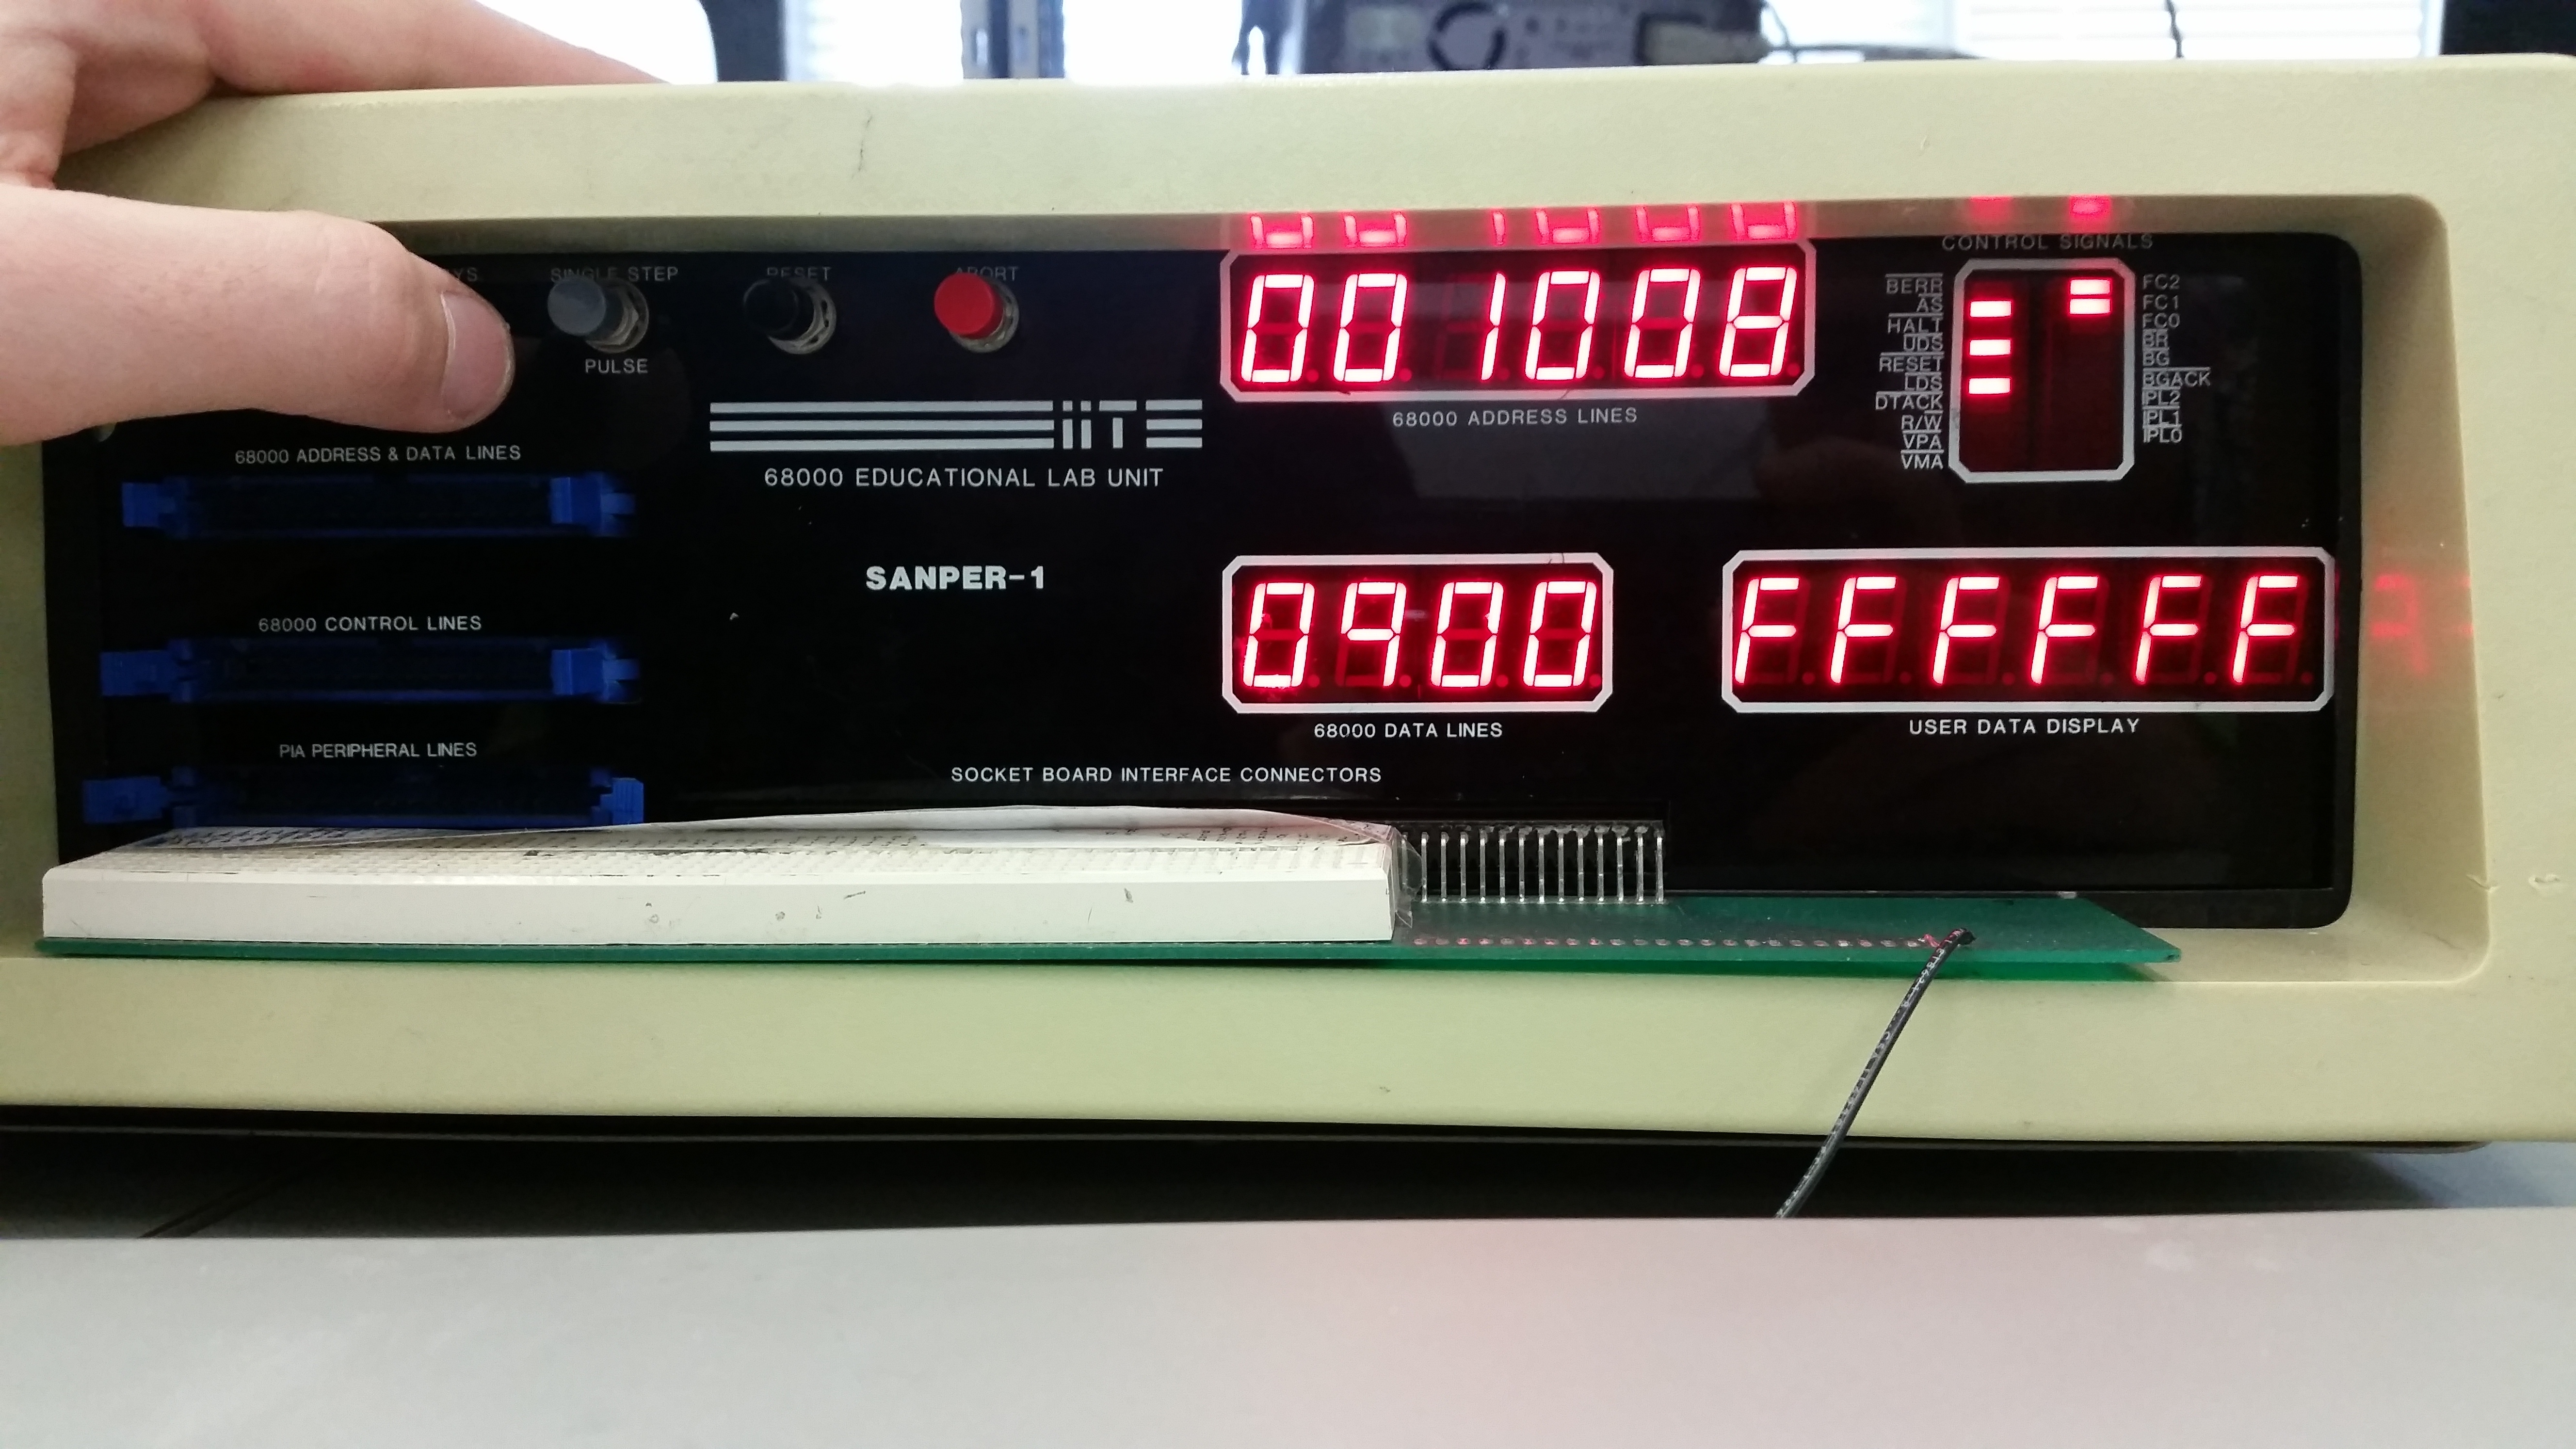
\includegraphics[width=1\linewidth]{Lab1/20150120_093605}
\end{center}
\begin{center}
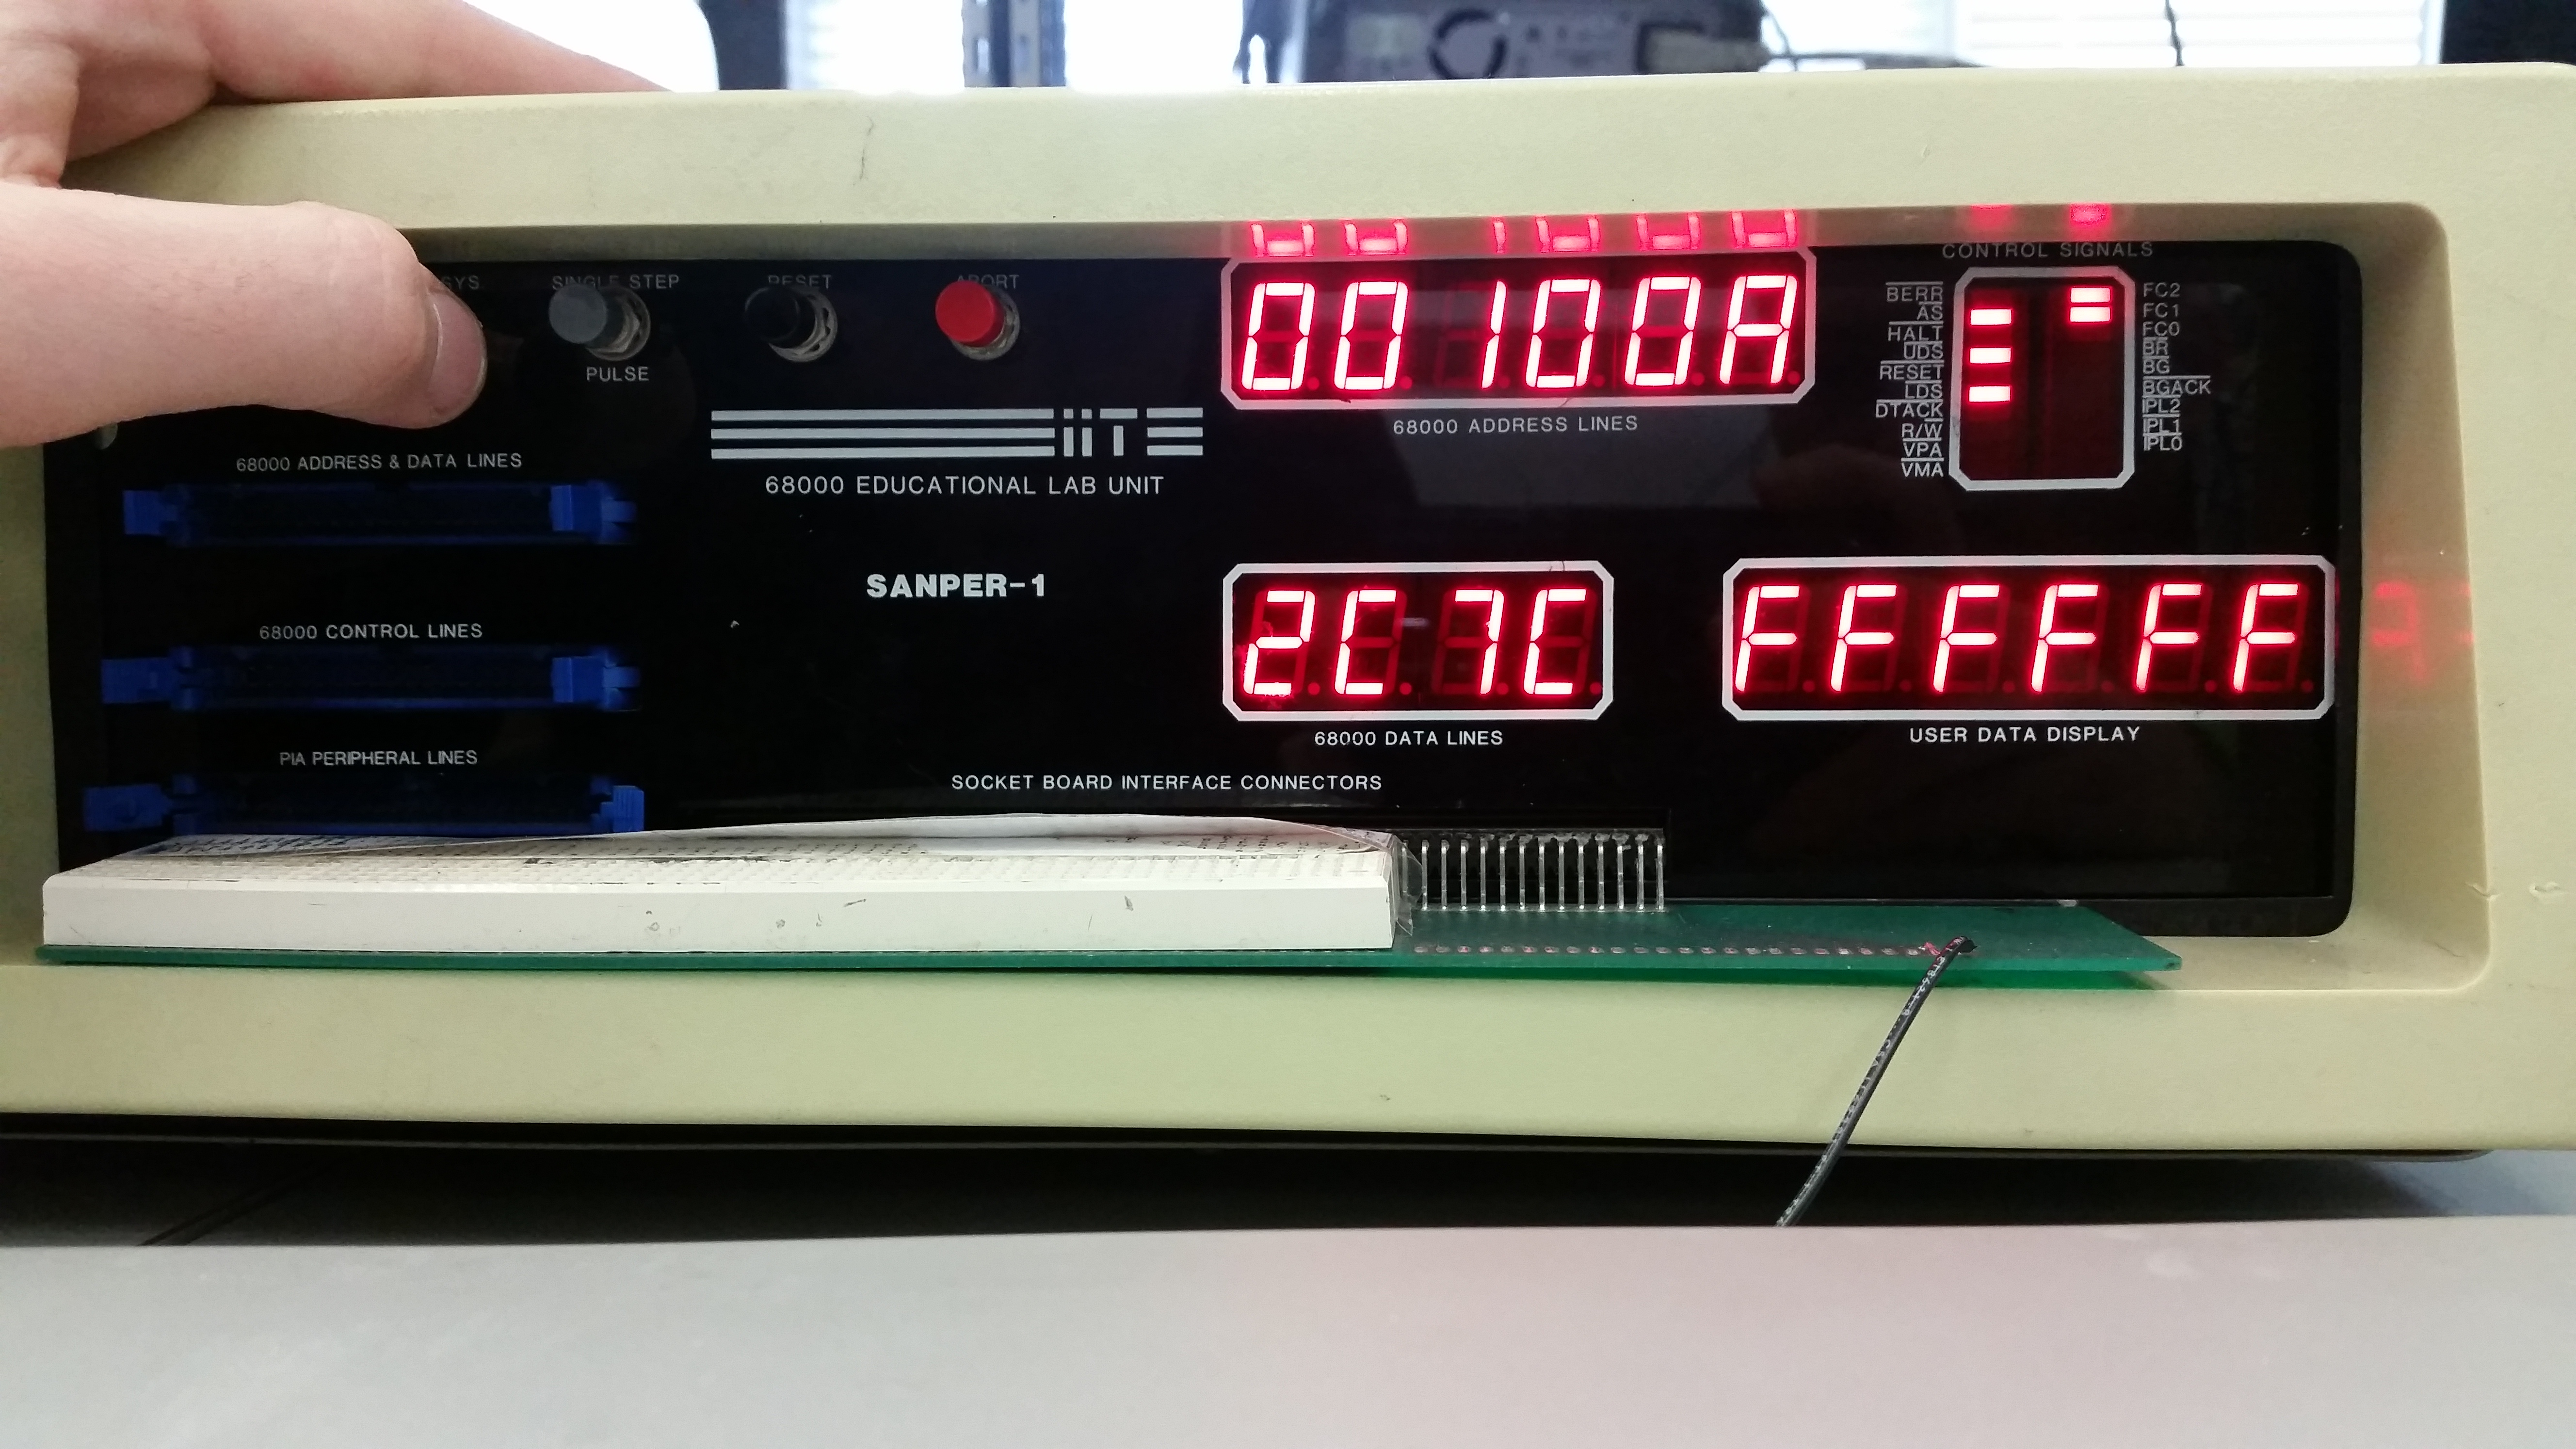
\includegraphics[width=1\linewidth]{Lab1/20150120_093608}
\end{center}
\begin{center}
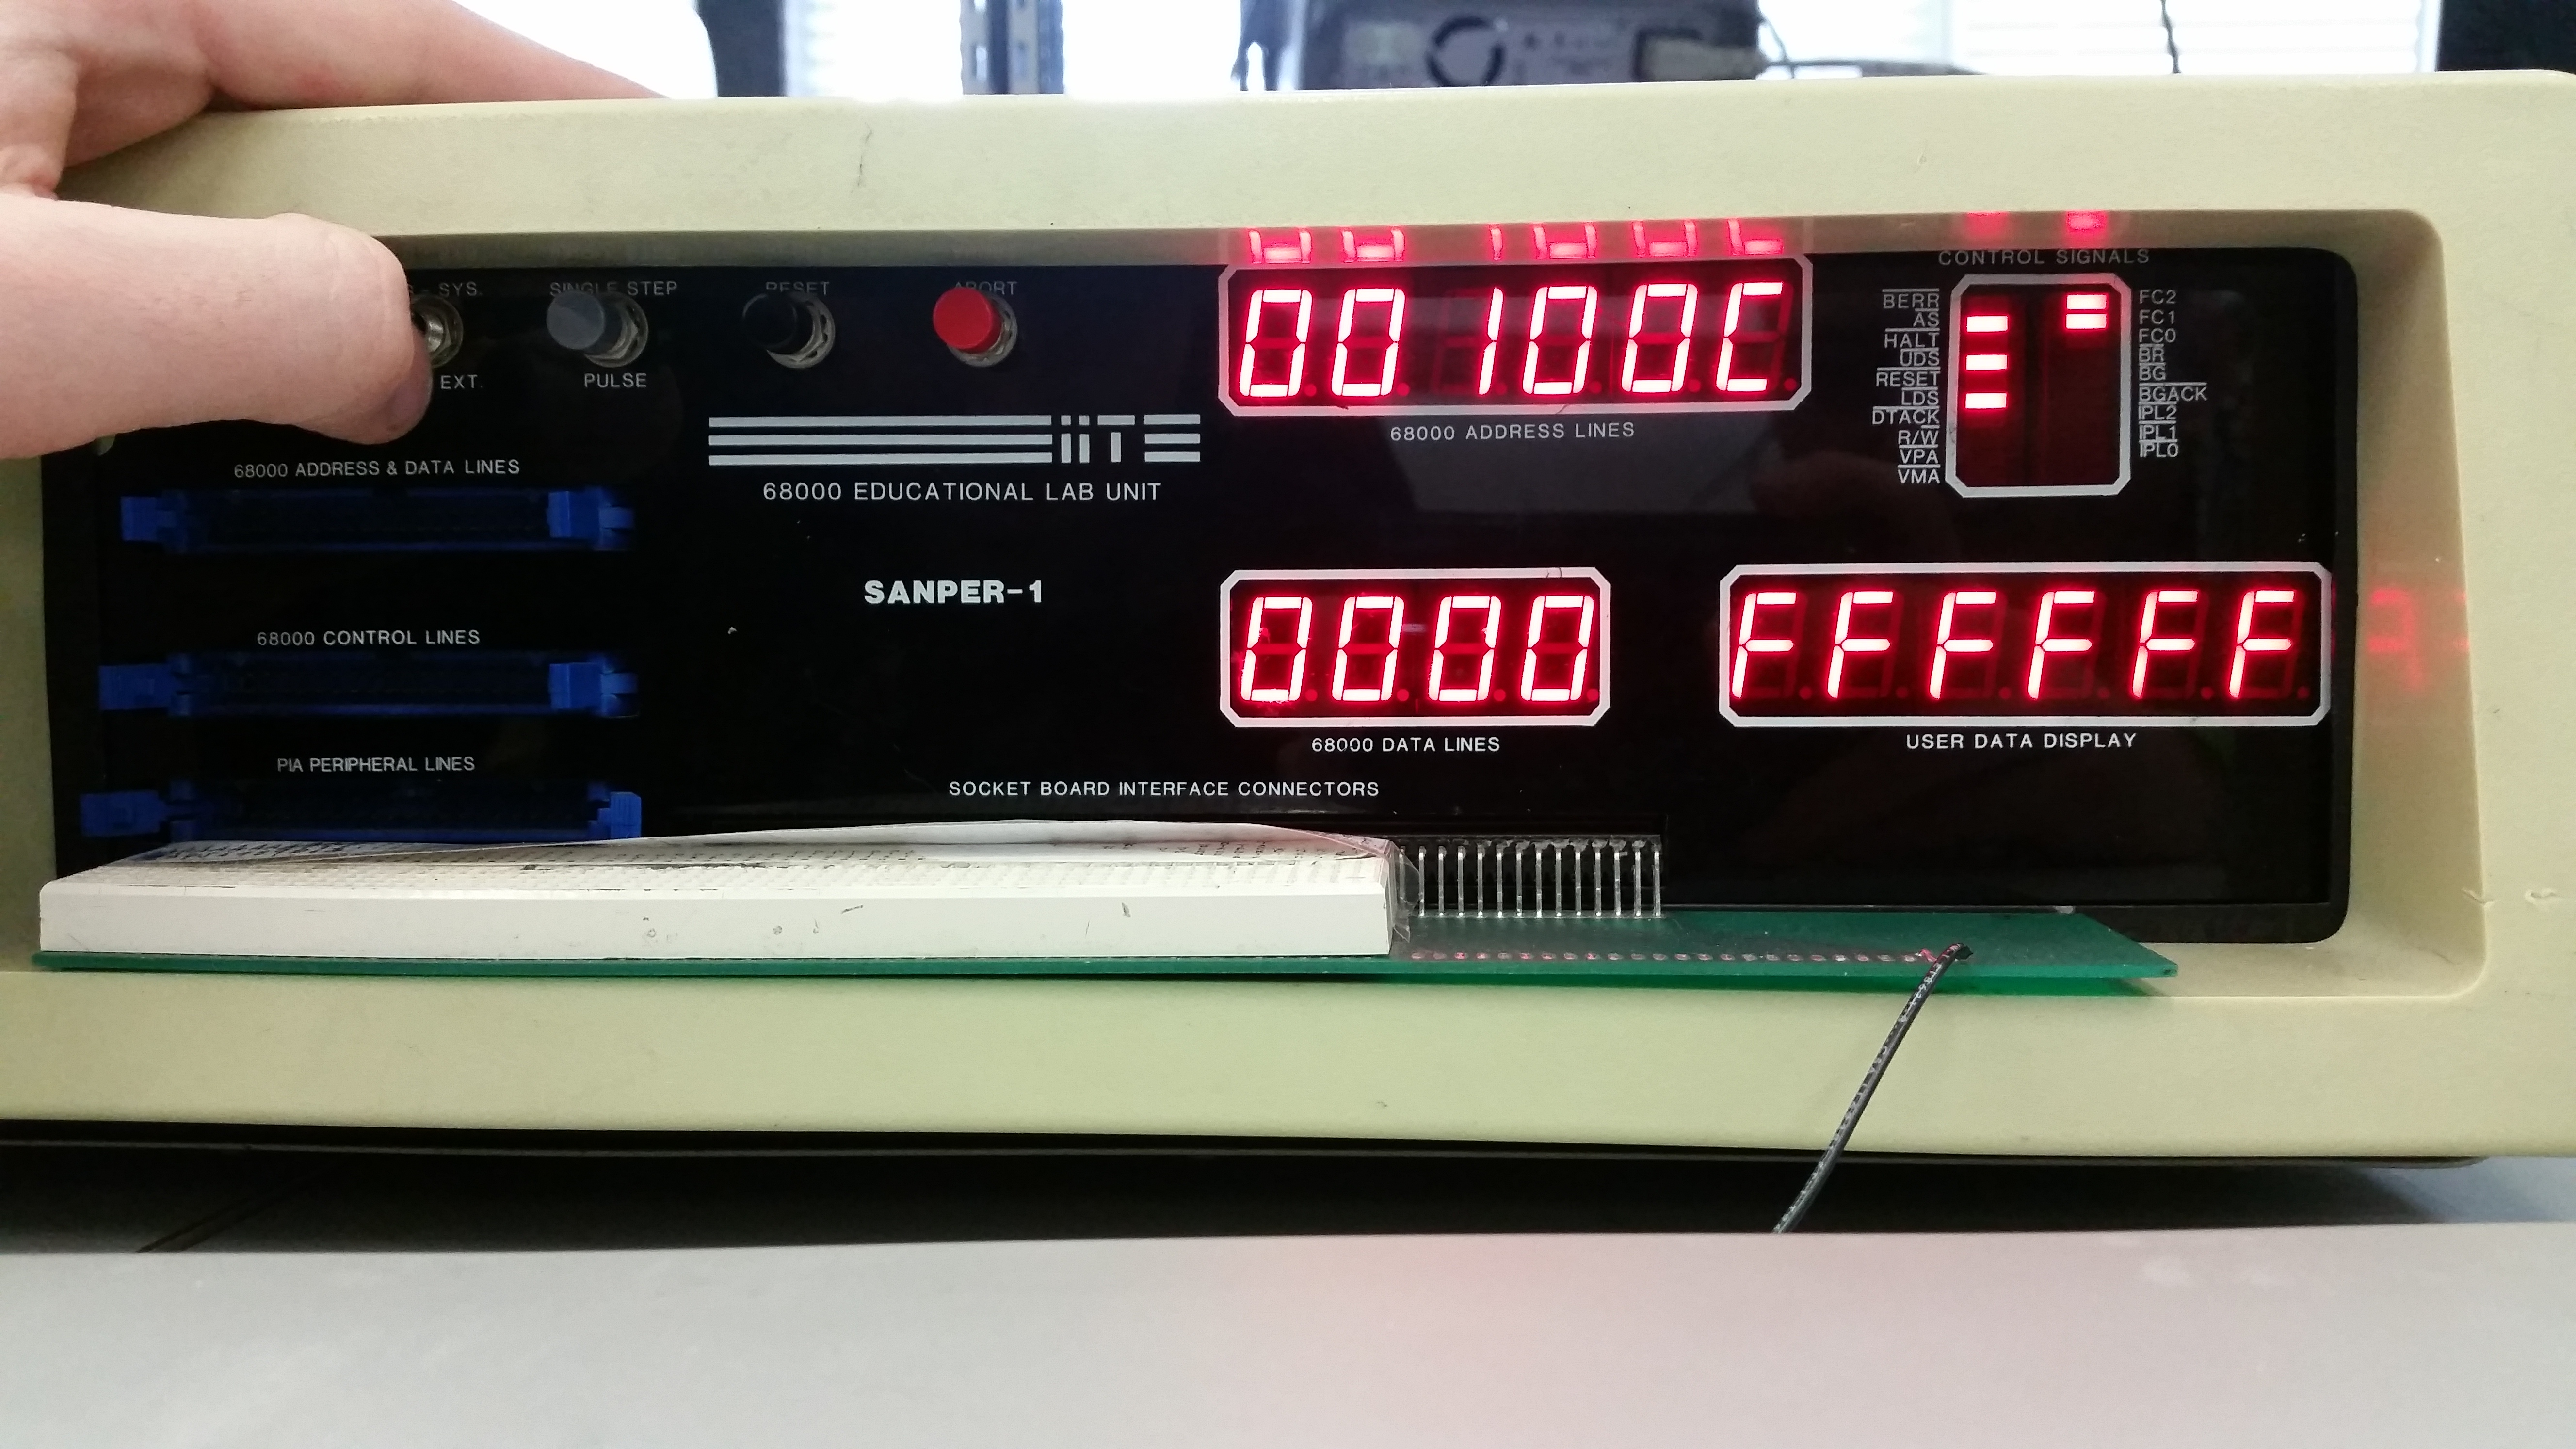
\includegraphics[width=1\linewidth]{Lab1/20150120_093610}
\end{center}
\begin{center}
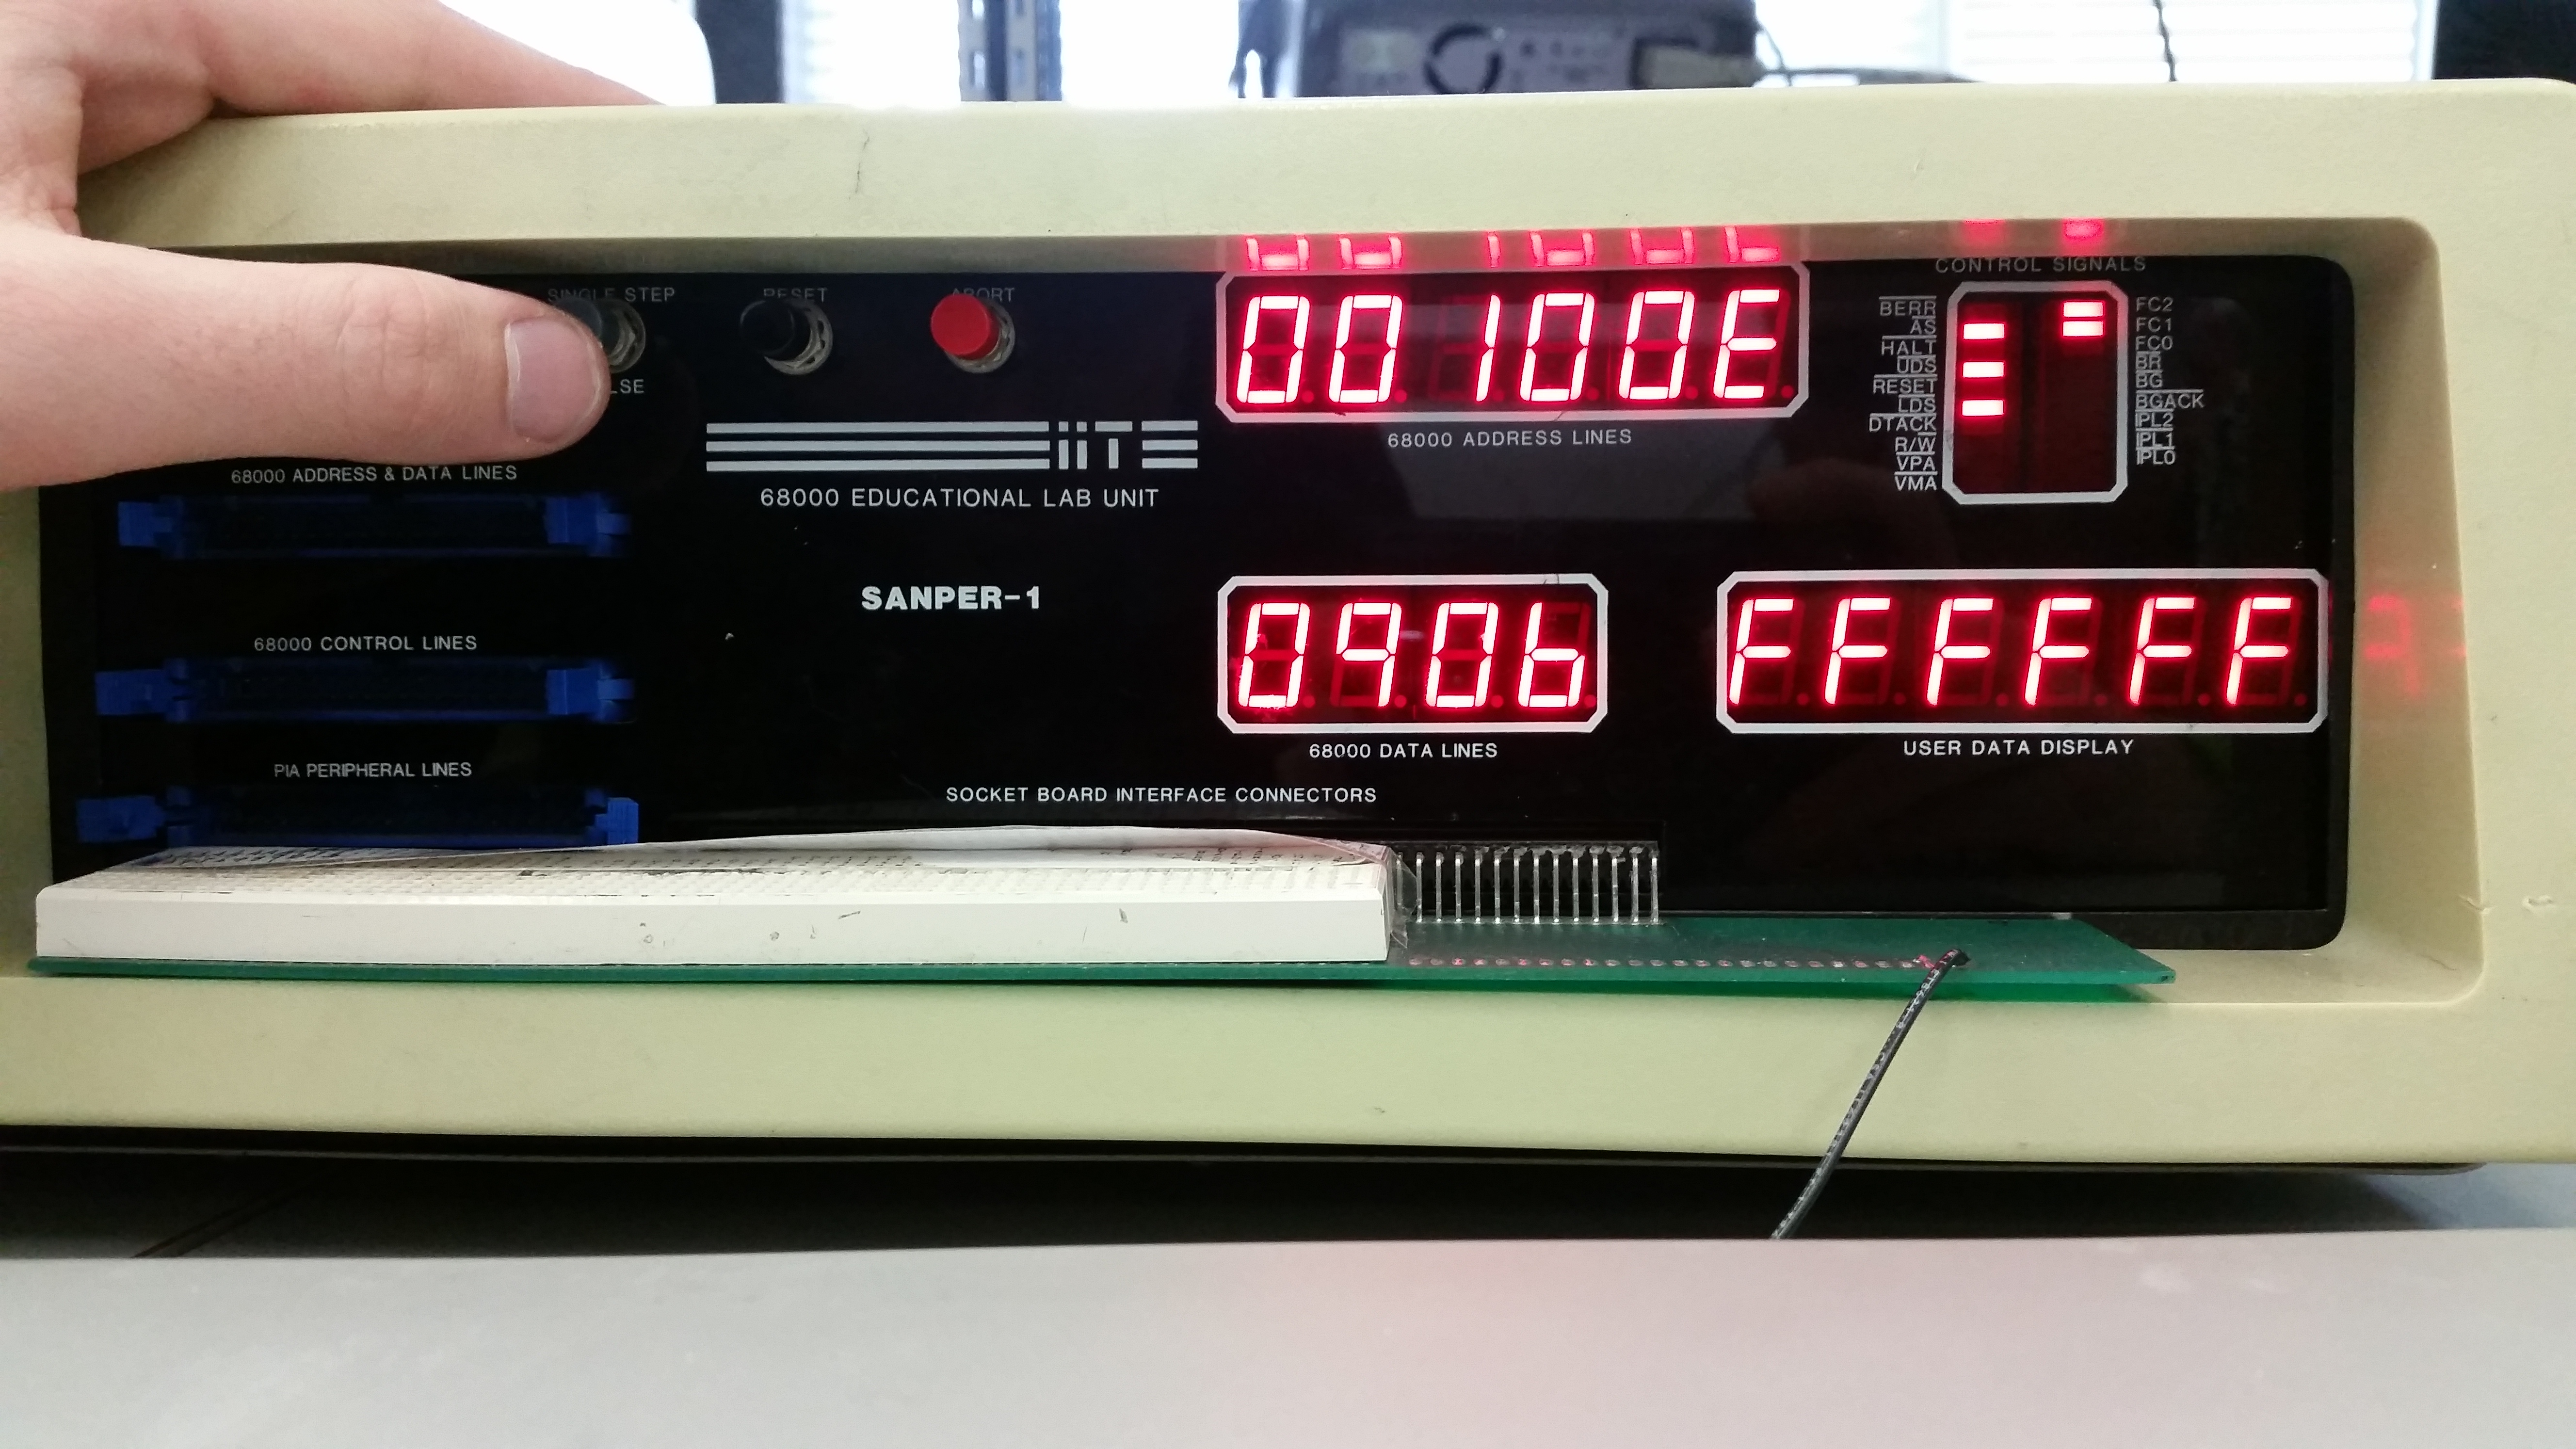
\includegraphics[width=1\linewidth]{Lab1/20150120_093612}
\end{center}
\begin{center}
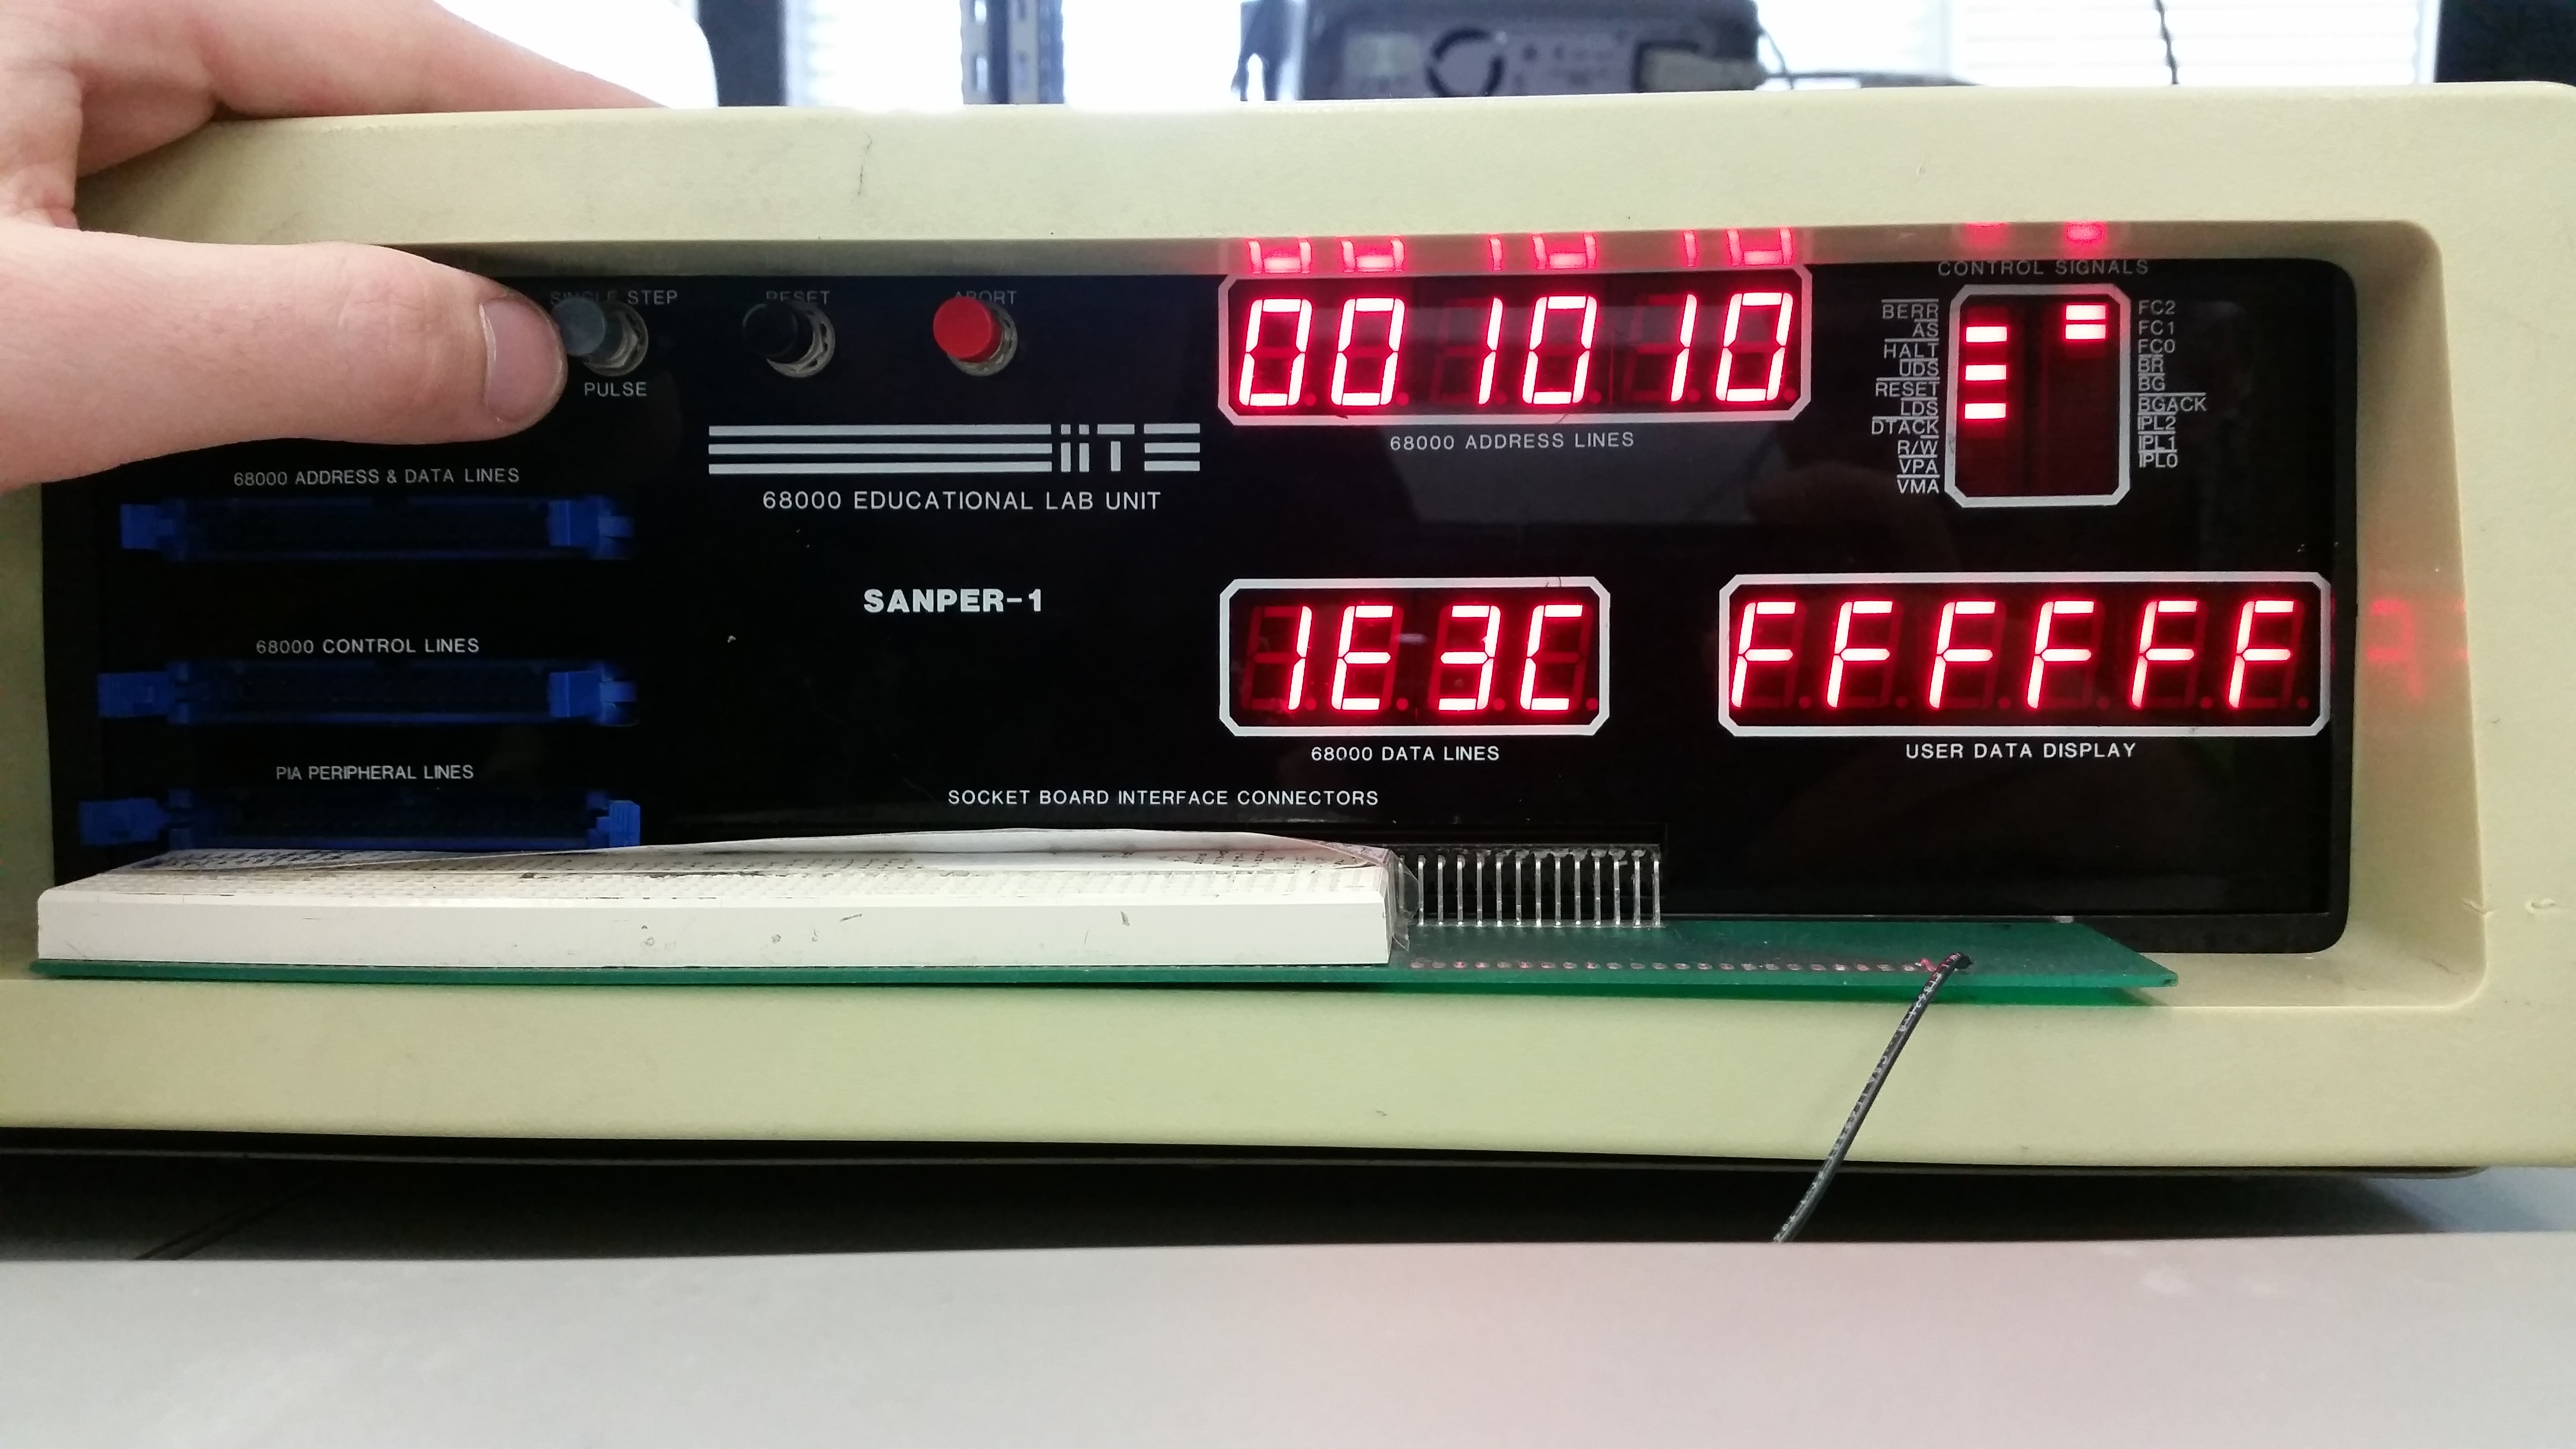
\includegraphics[width=1\linewidth]{Lab1/20150120_093614}
\end{center}
\begin{center}
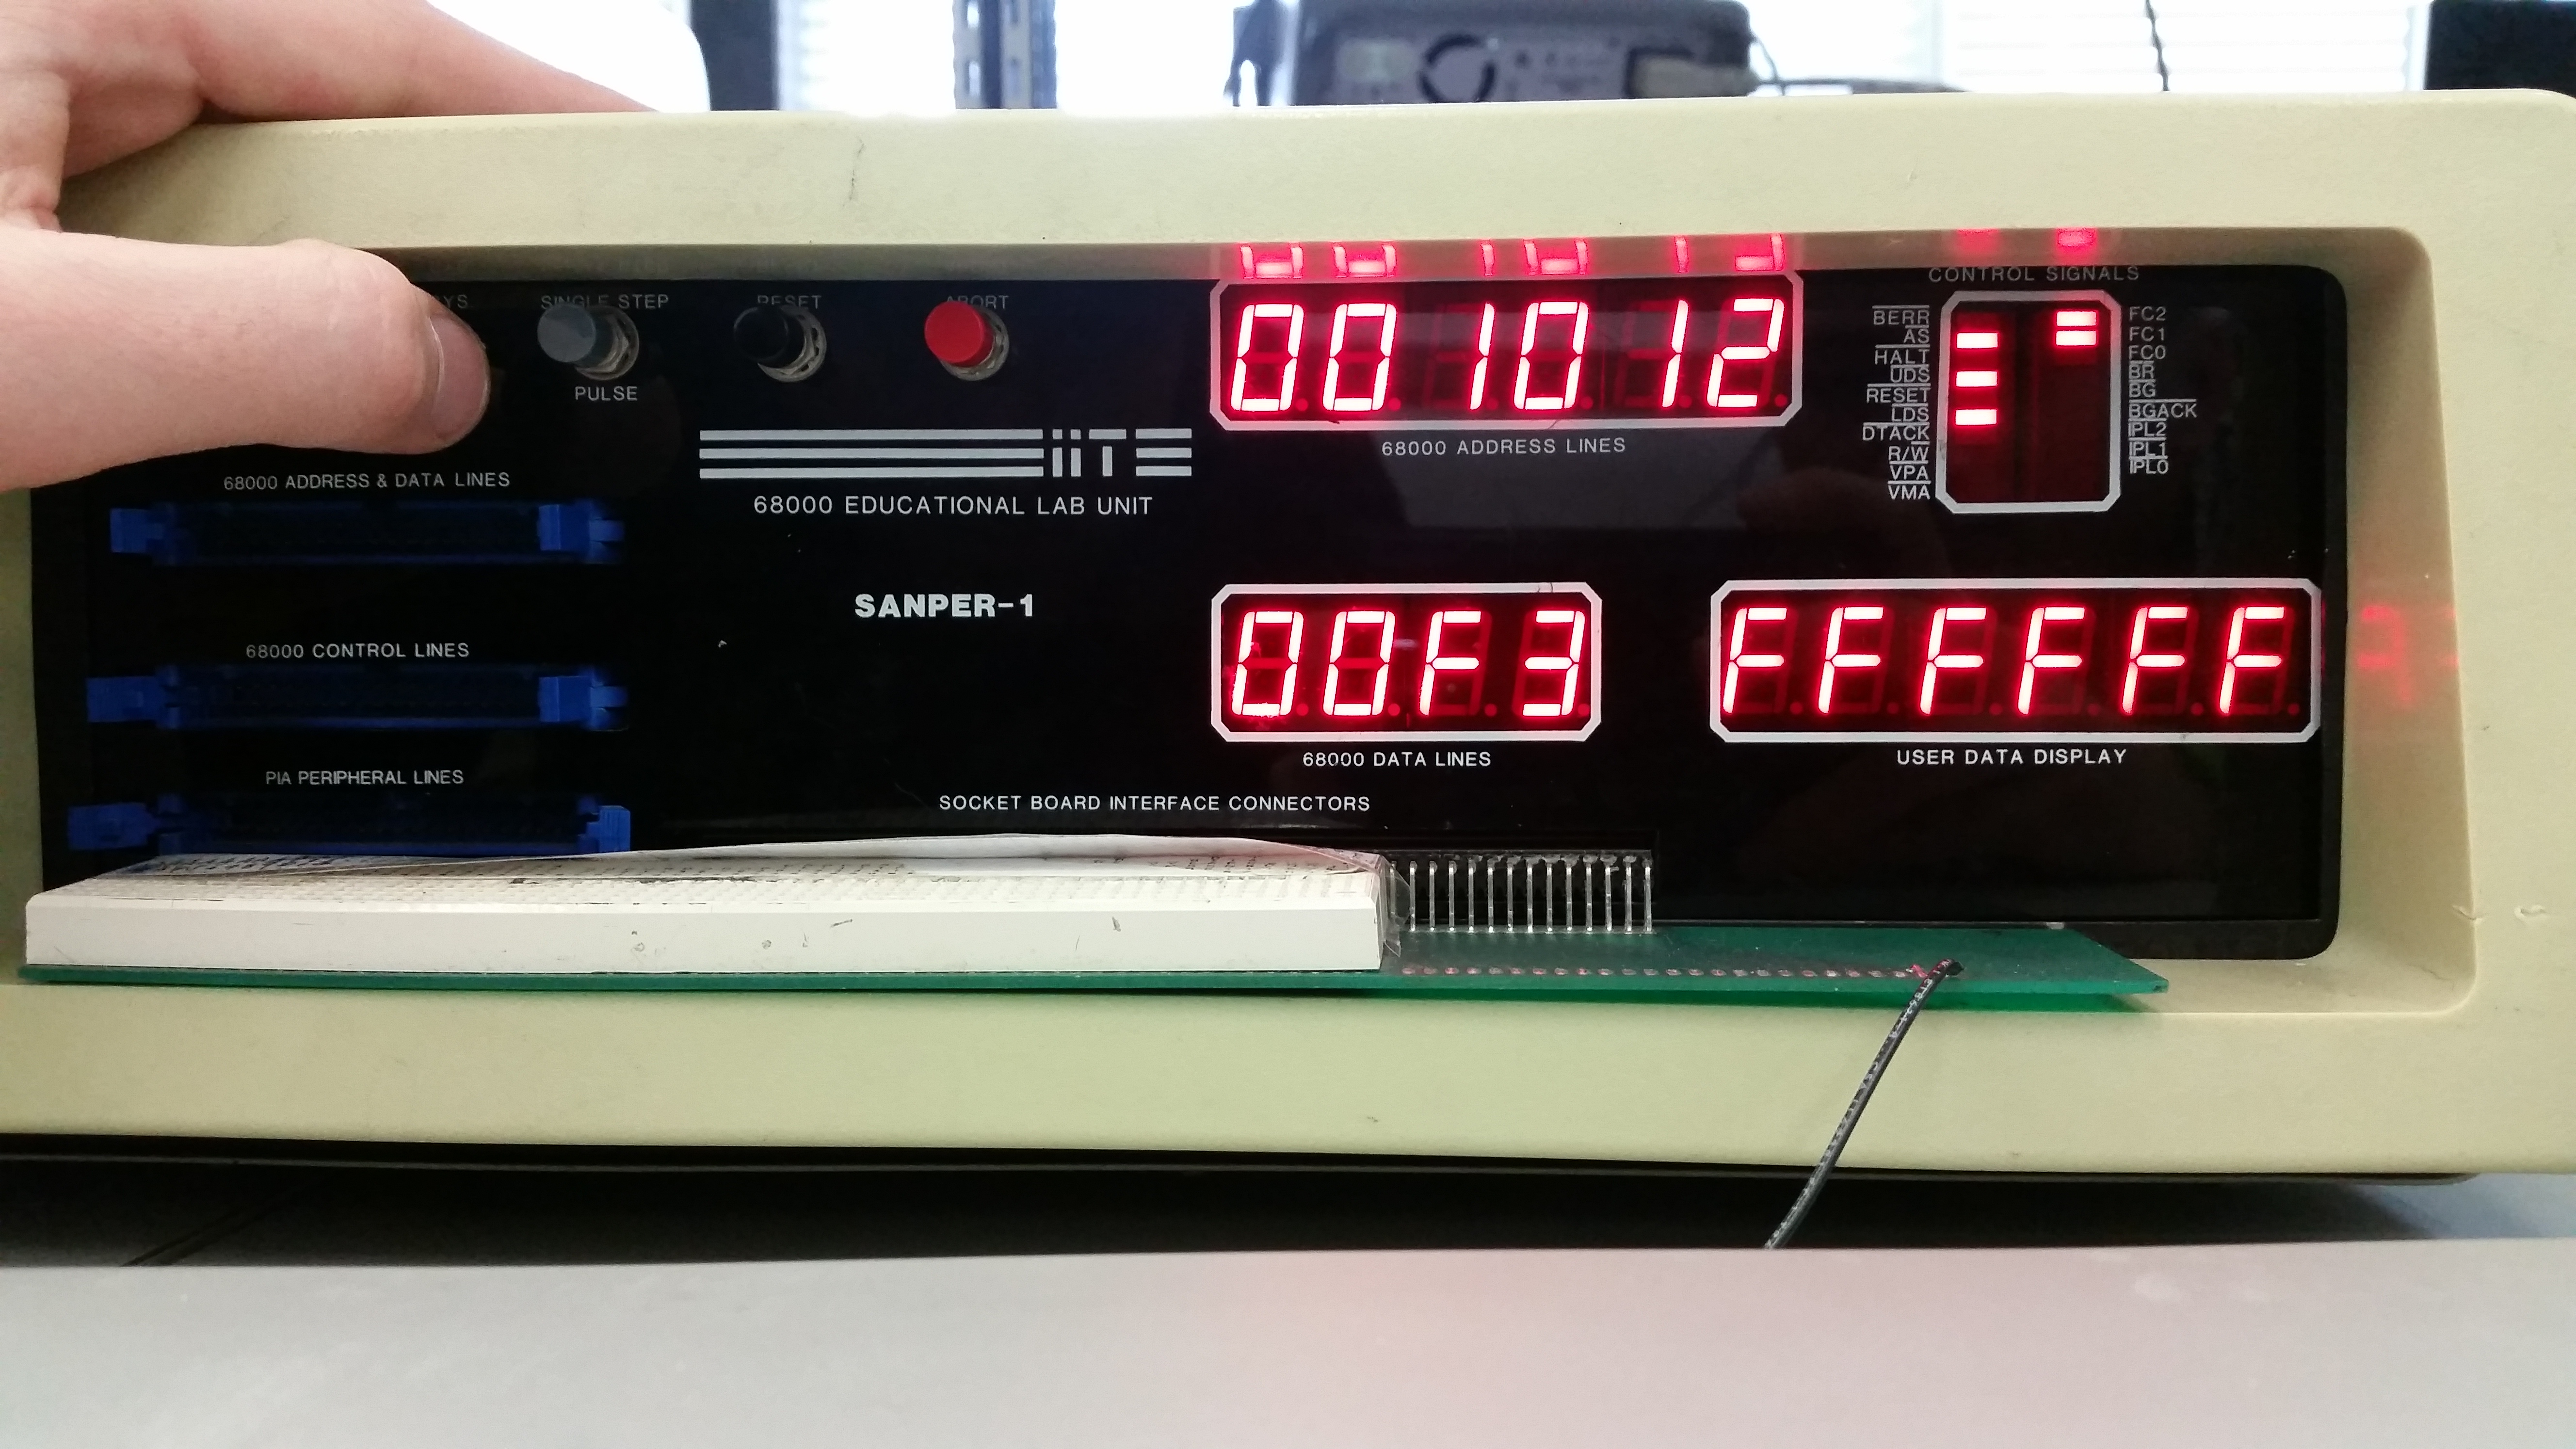
\includegraphics[width=1\linewidth]{Lab1/20150120_093616}
\end{center}
\begin{center}
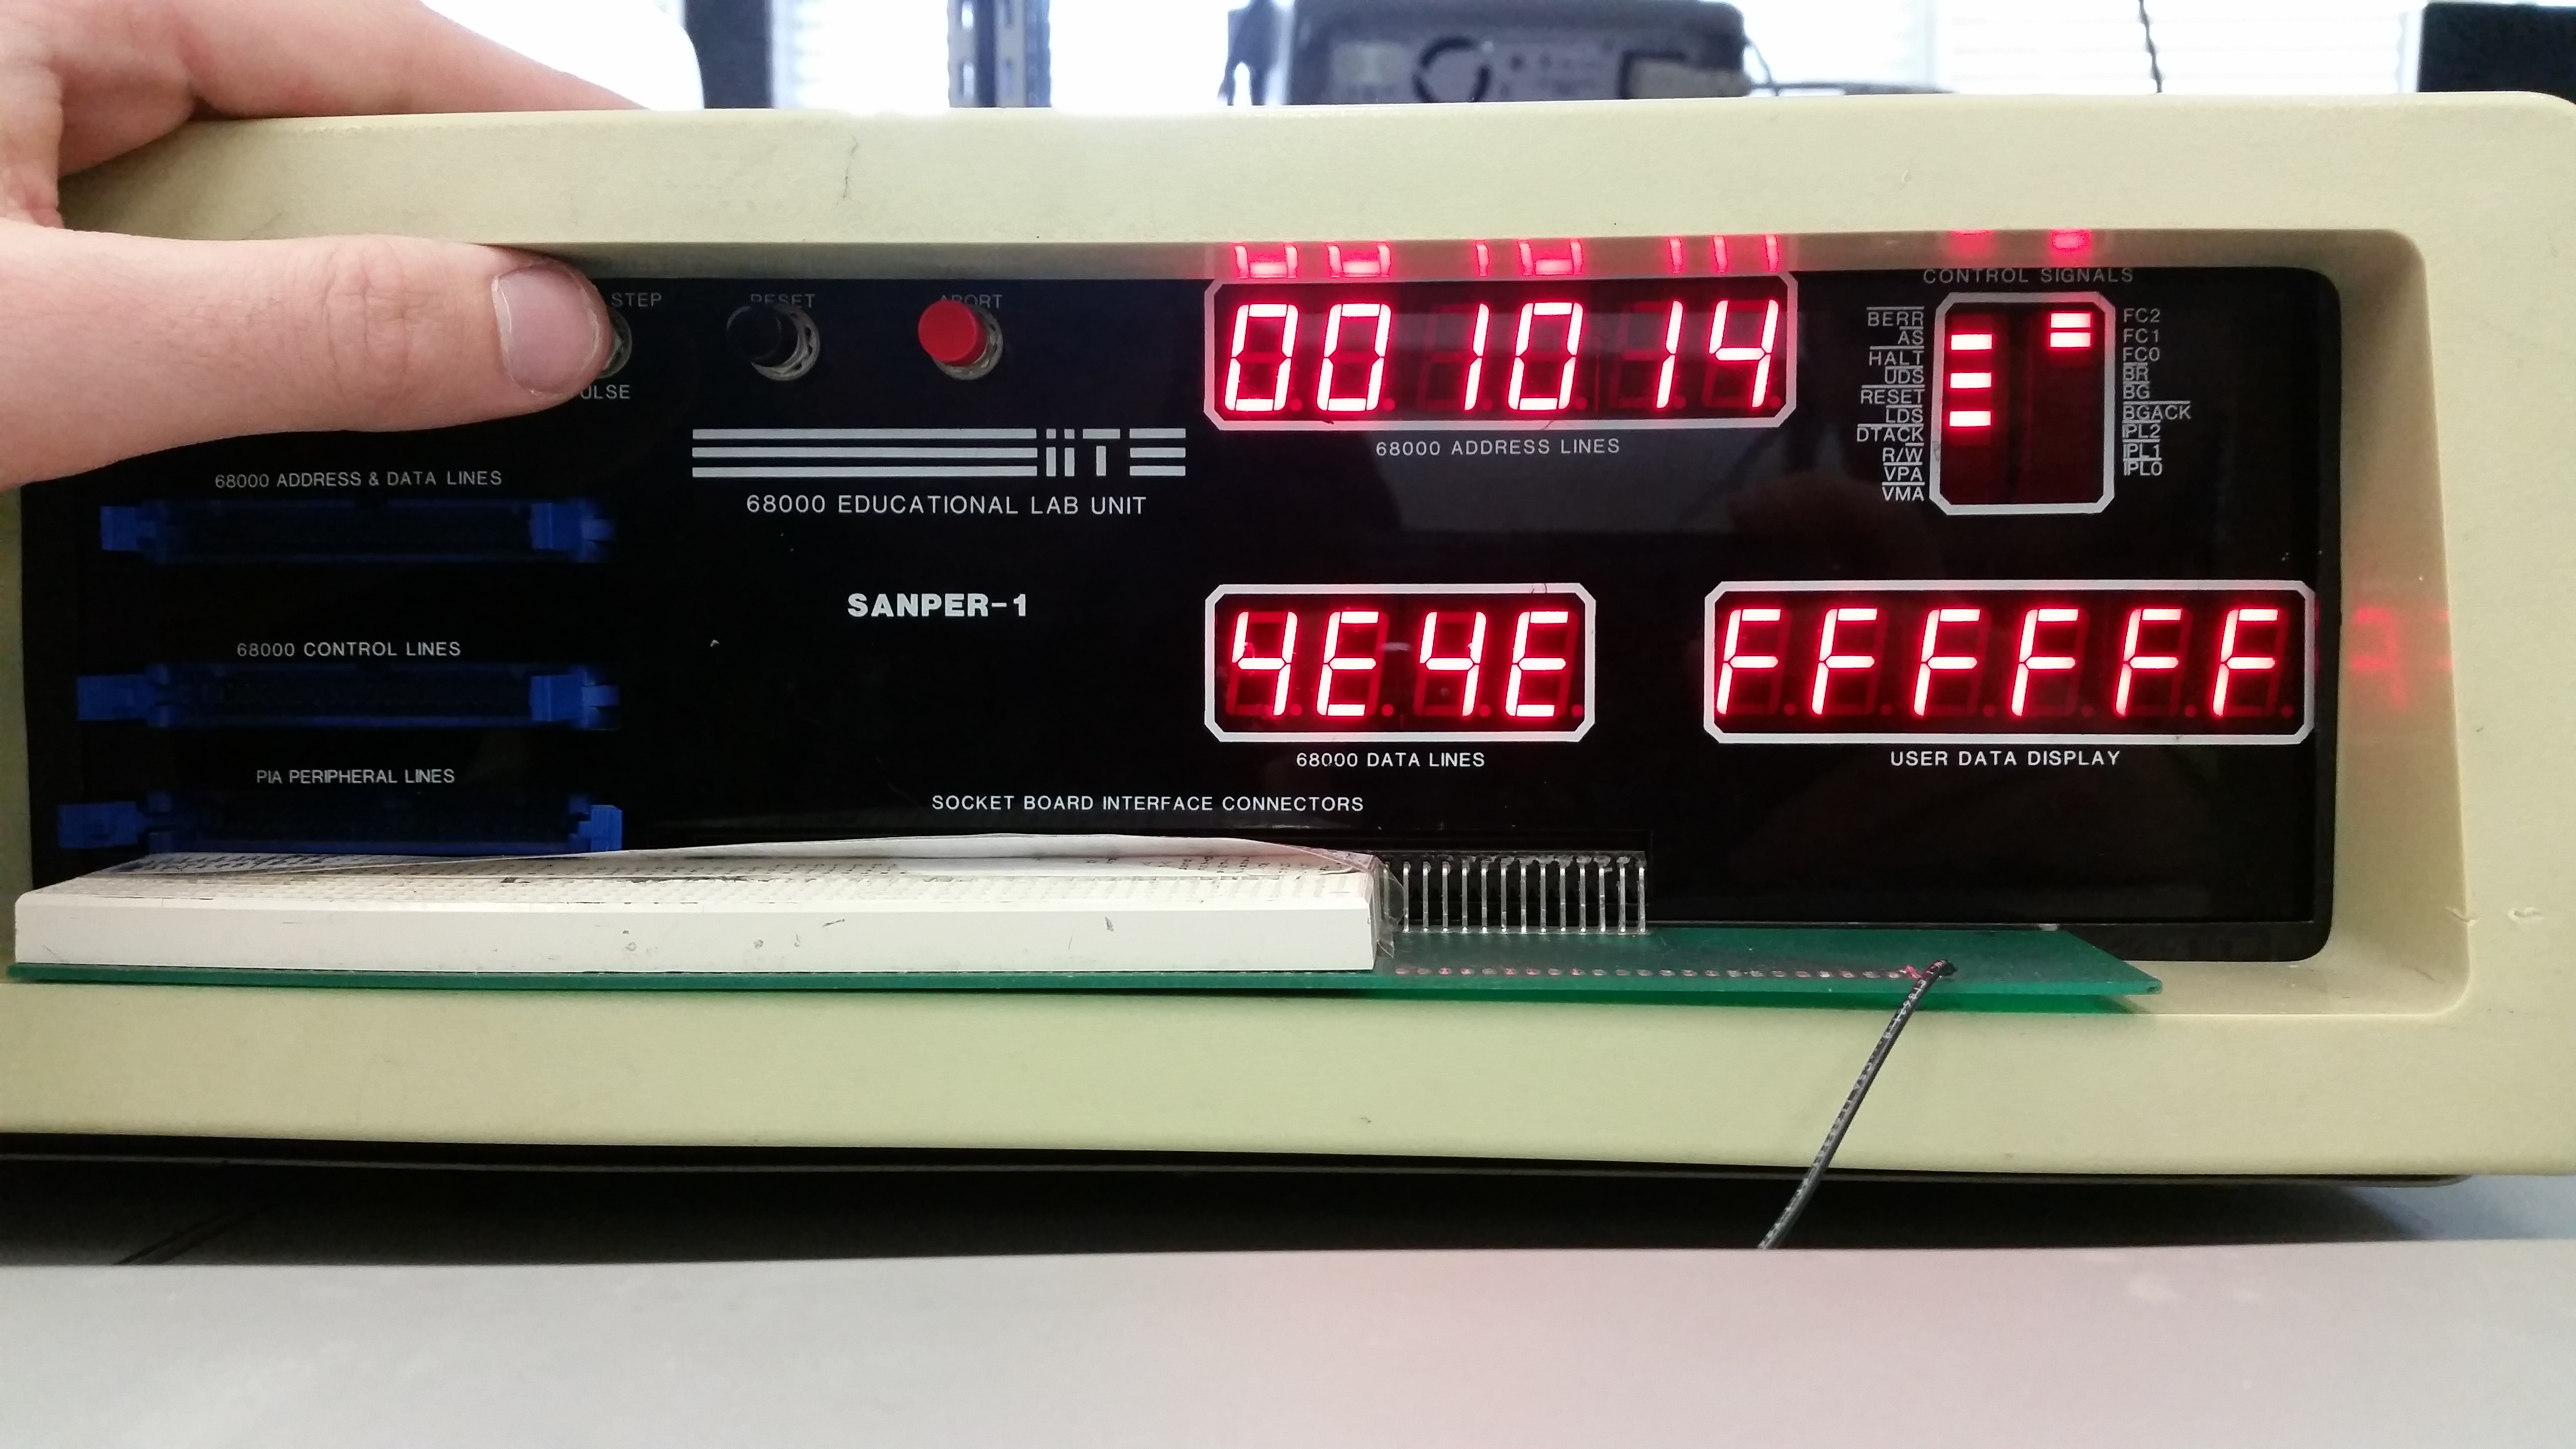
\includegraphics[width=1\linewidth]{Lab1/20150120_093618}
\end{center}
\begin{center}
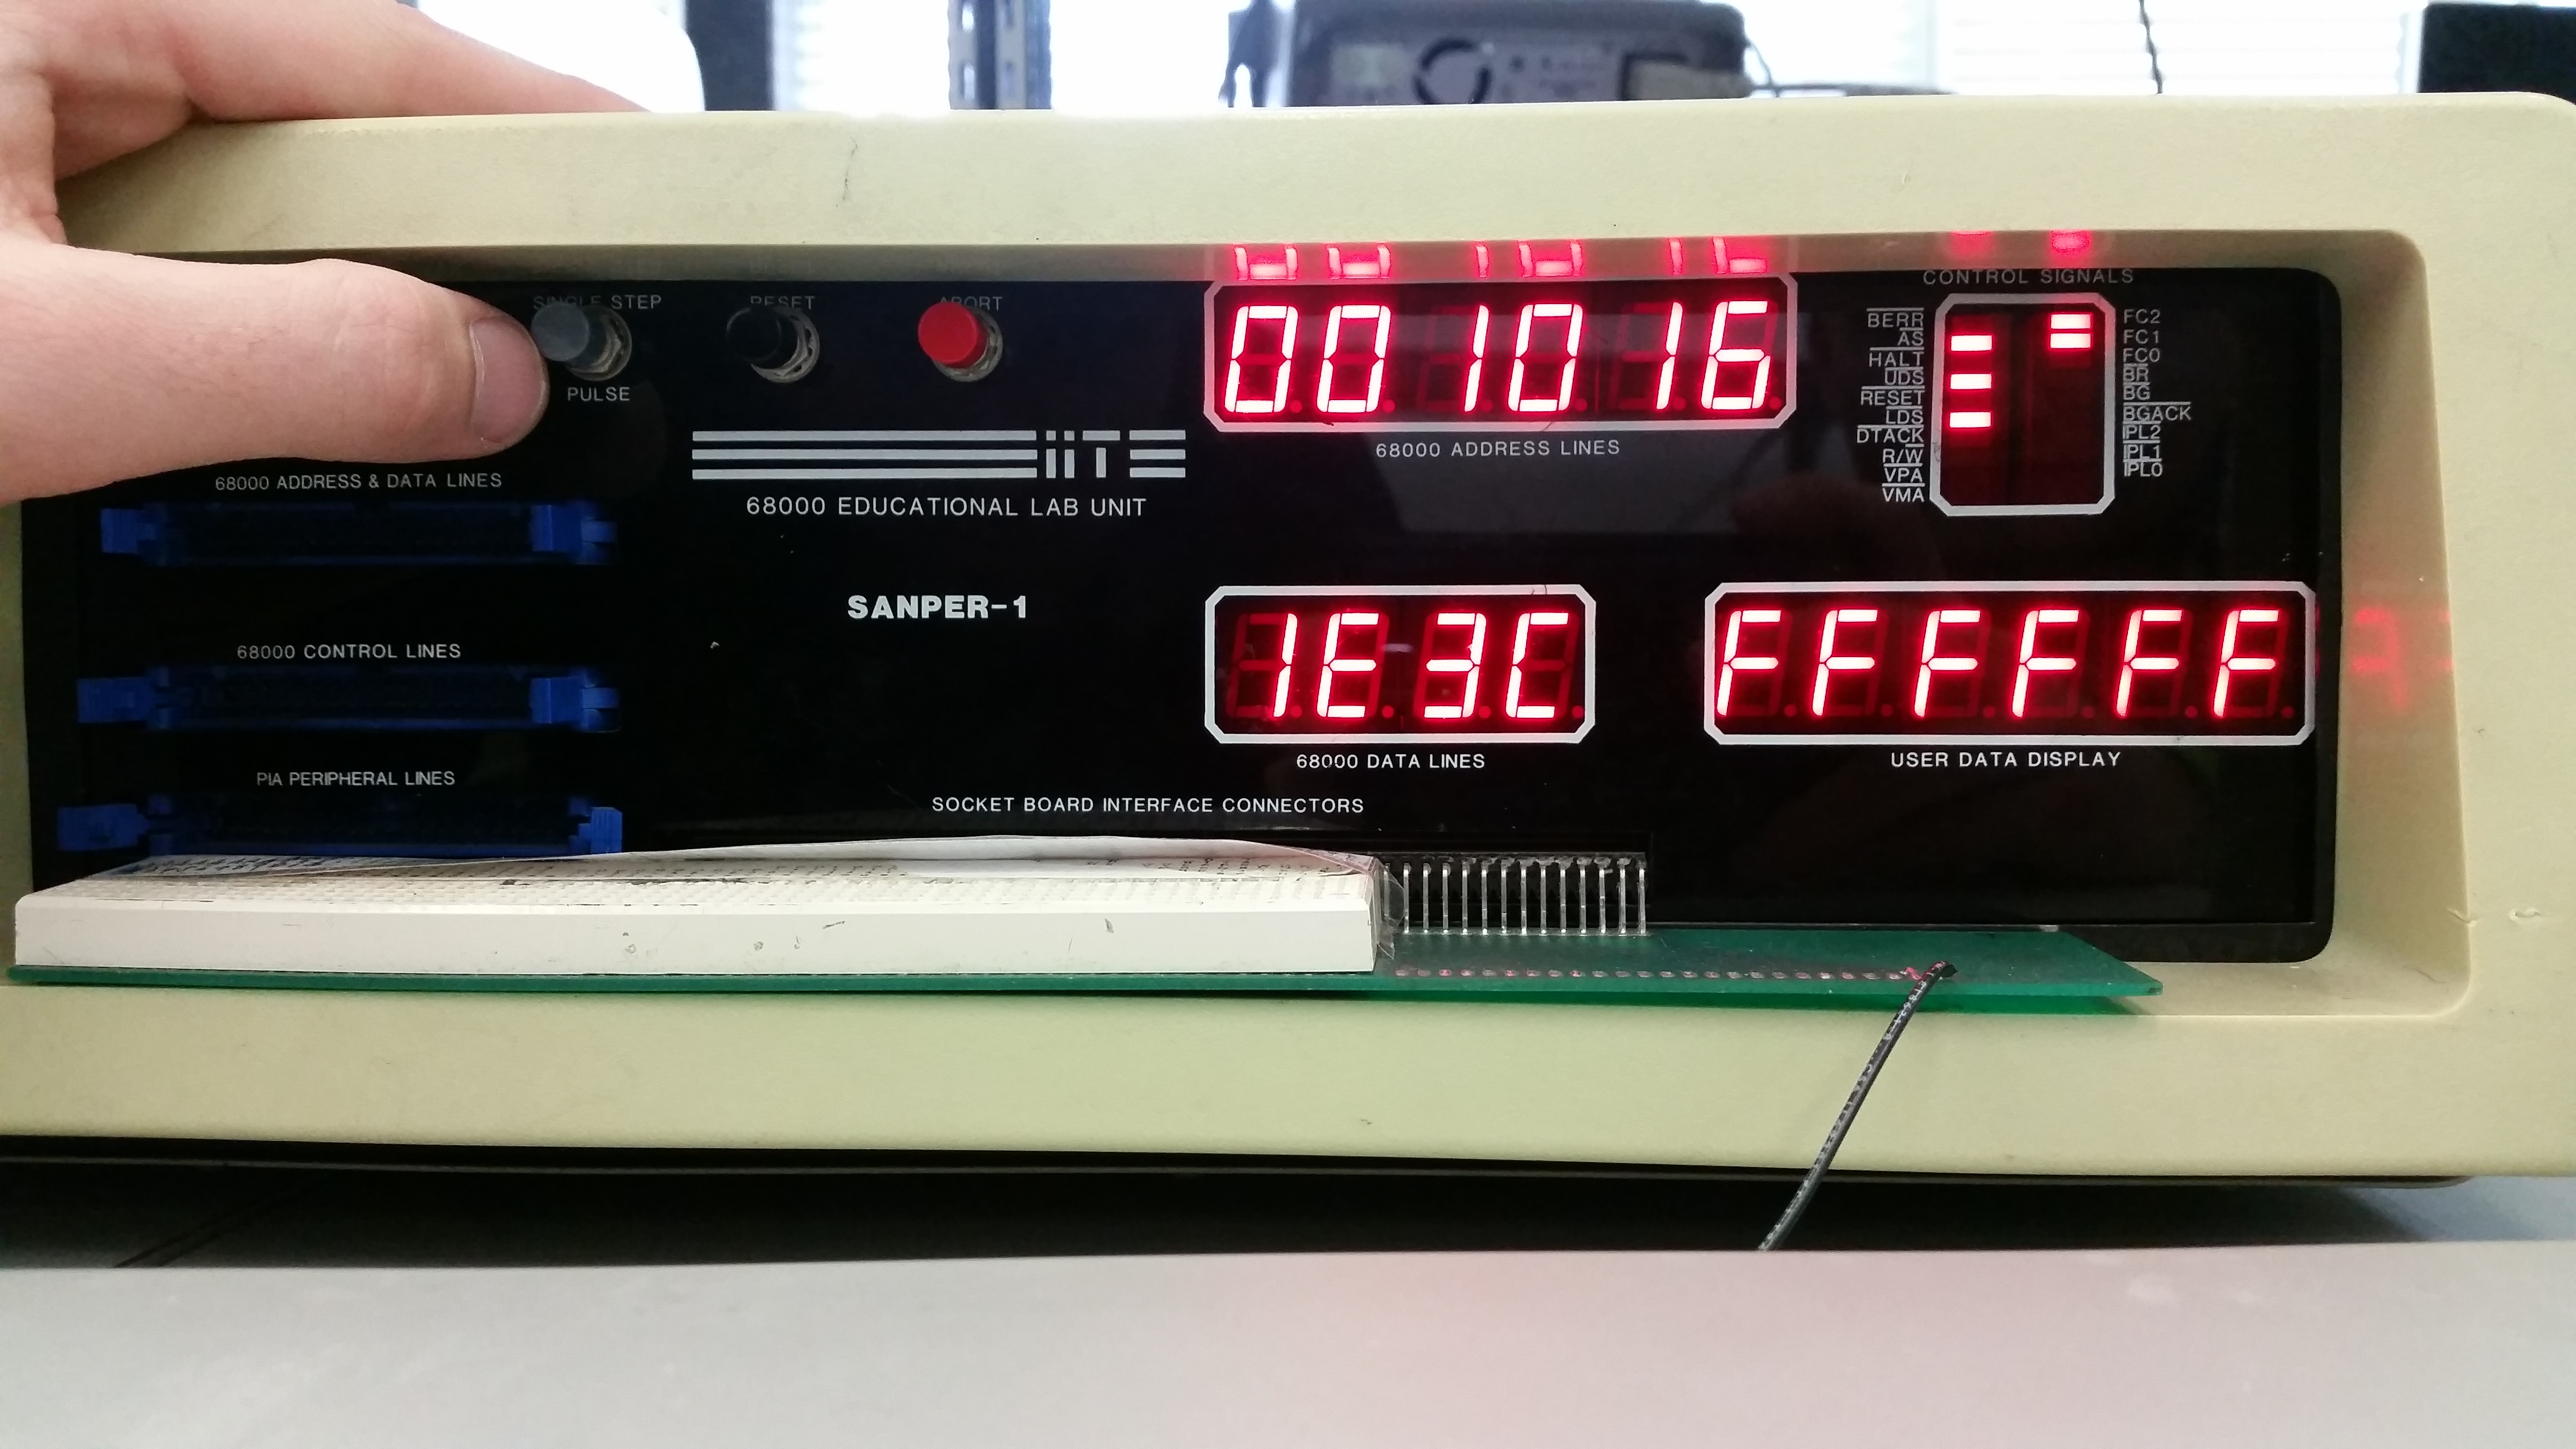
\includegraphics[width=1\linewidth]{Lab1/20150120_093620}
\end{center}
\begin{center}
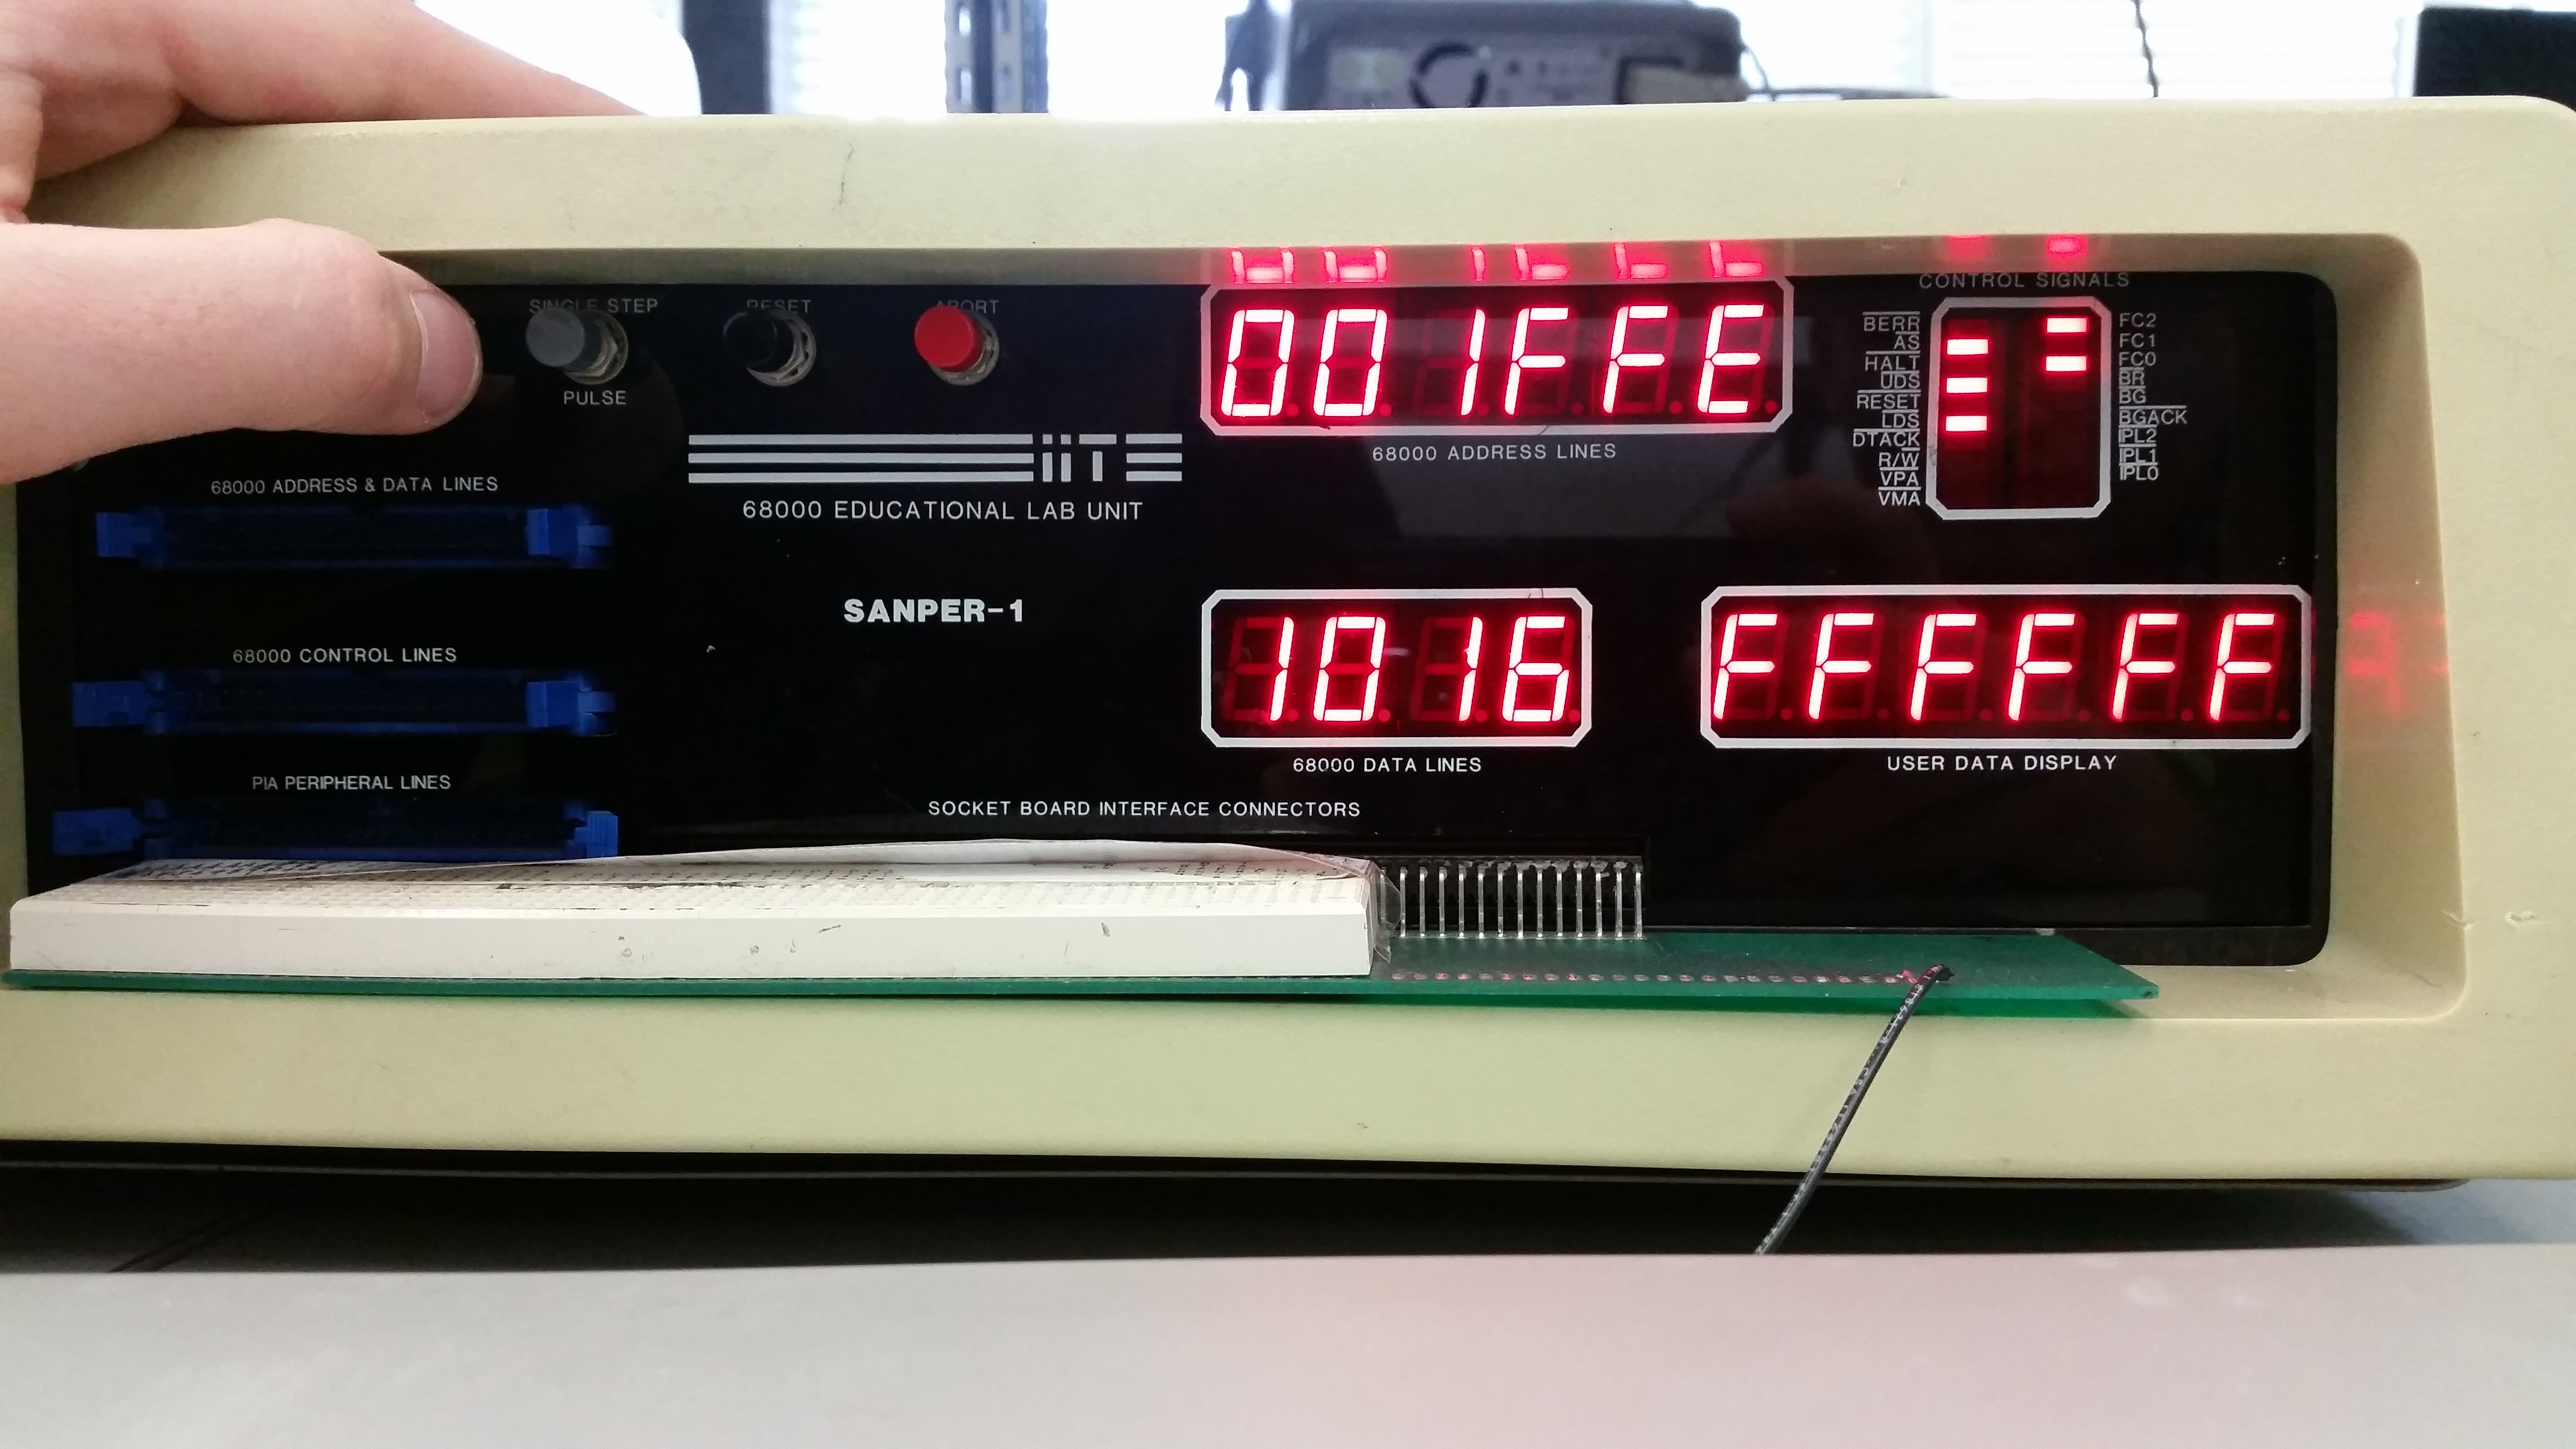
\includegraphics[width=1\linewidth]{Lab1/20150120_093621}
\end{center}
\subsubsection{Program 2}
\begin{center}
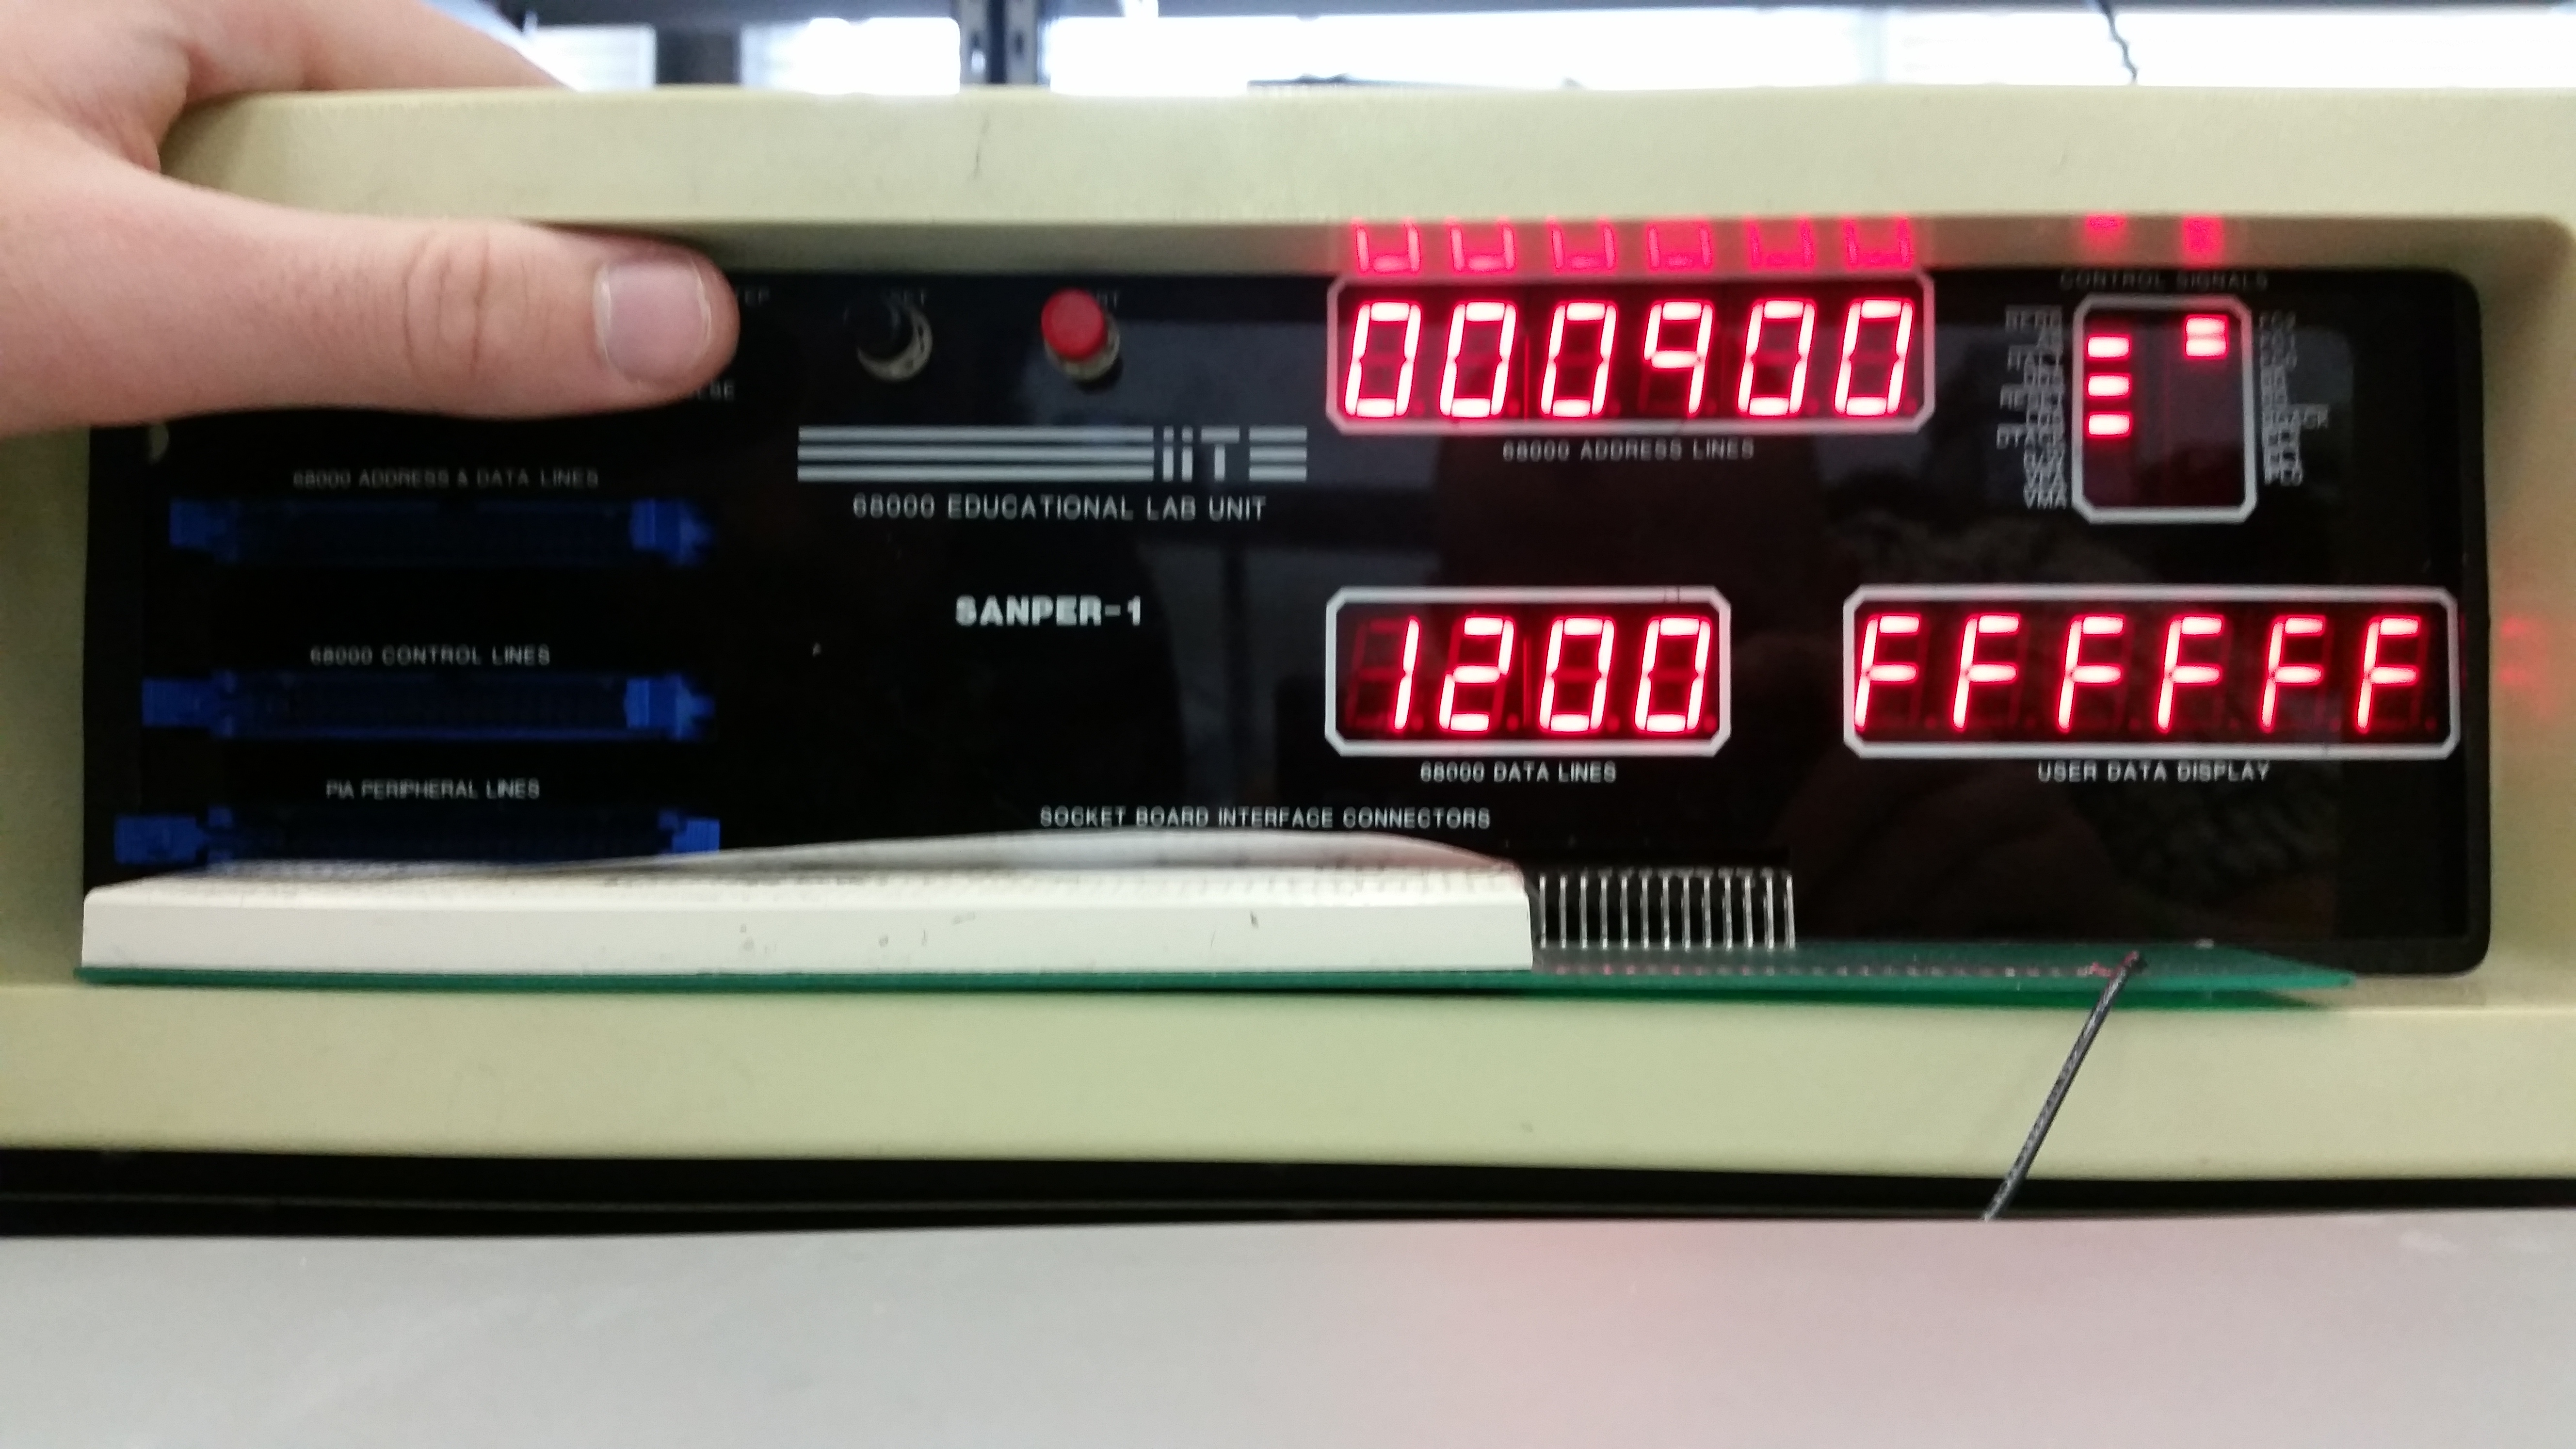
\includegraphics[width=1\linewidth]{Lab1/20150120_094136}
\end{center}
\begin{center}
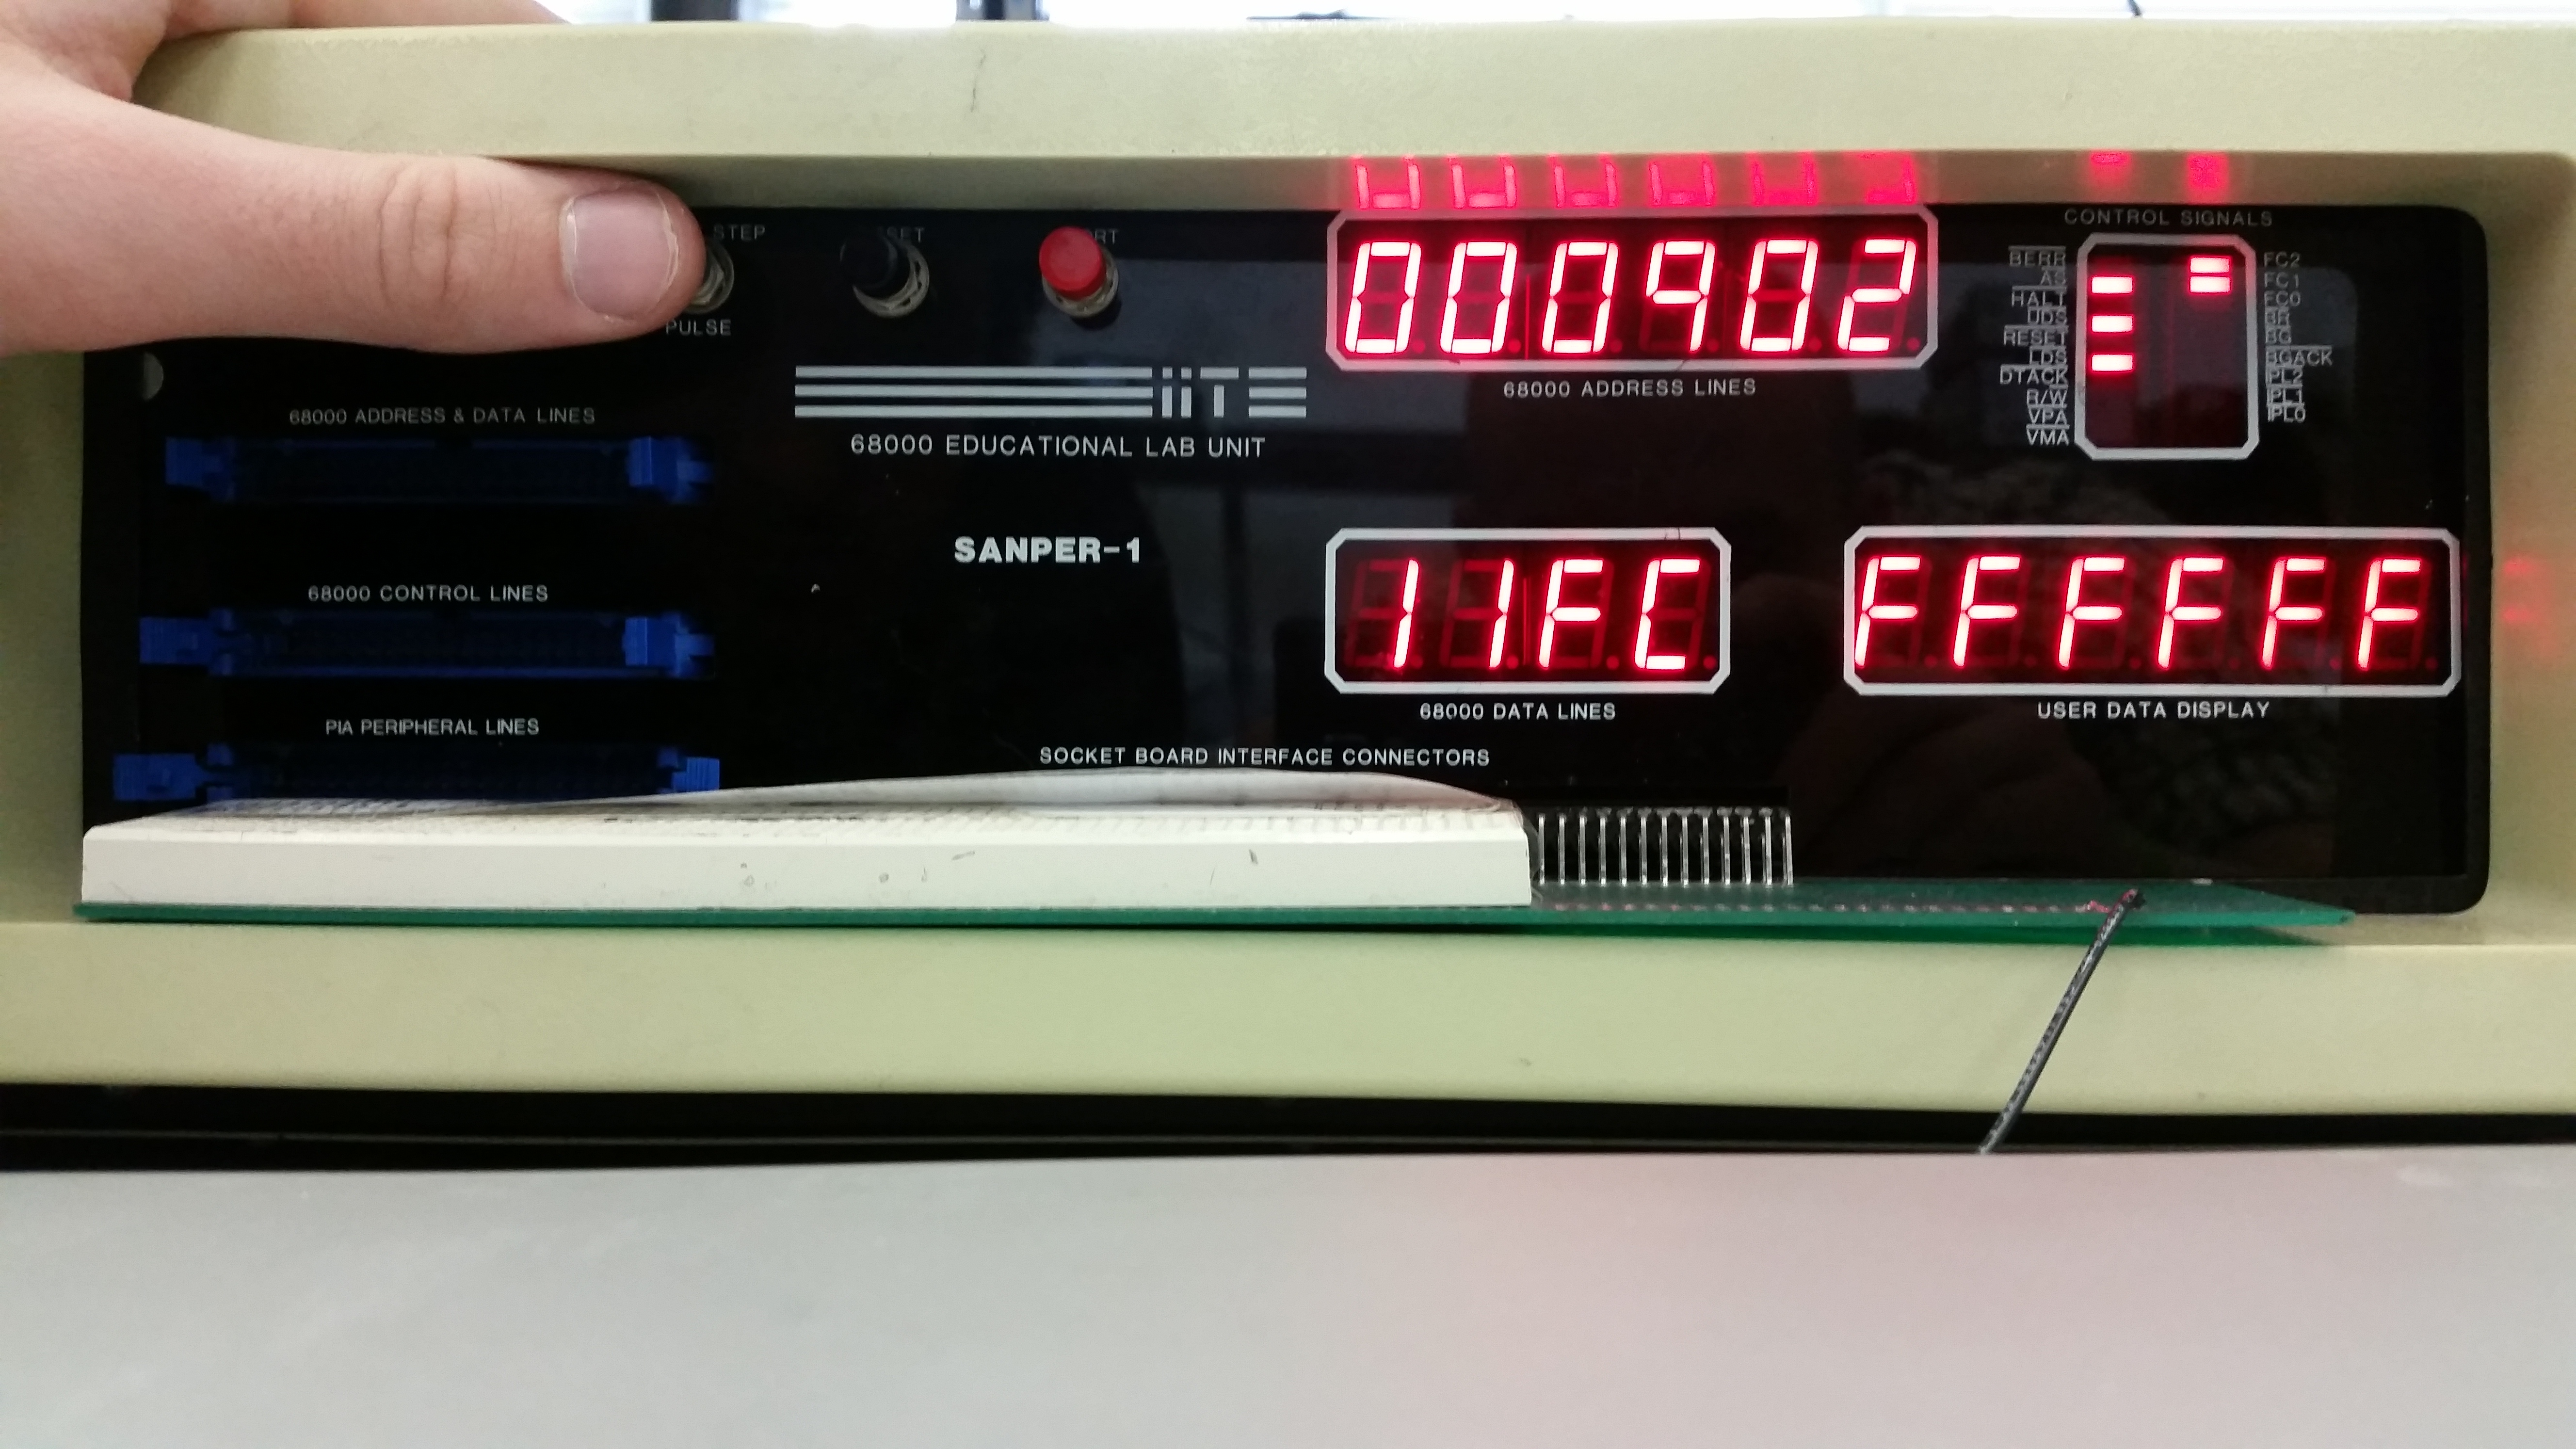
\includegraphics[width=1\linewidth]{Lab1/20150120_094138}
\end{center}
\begin{center}
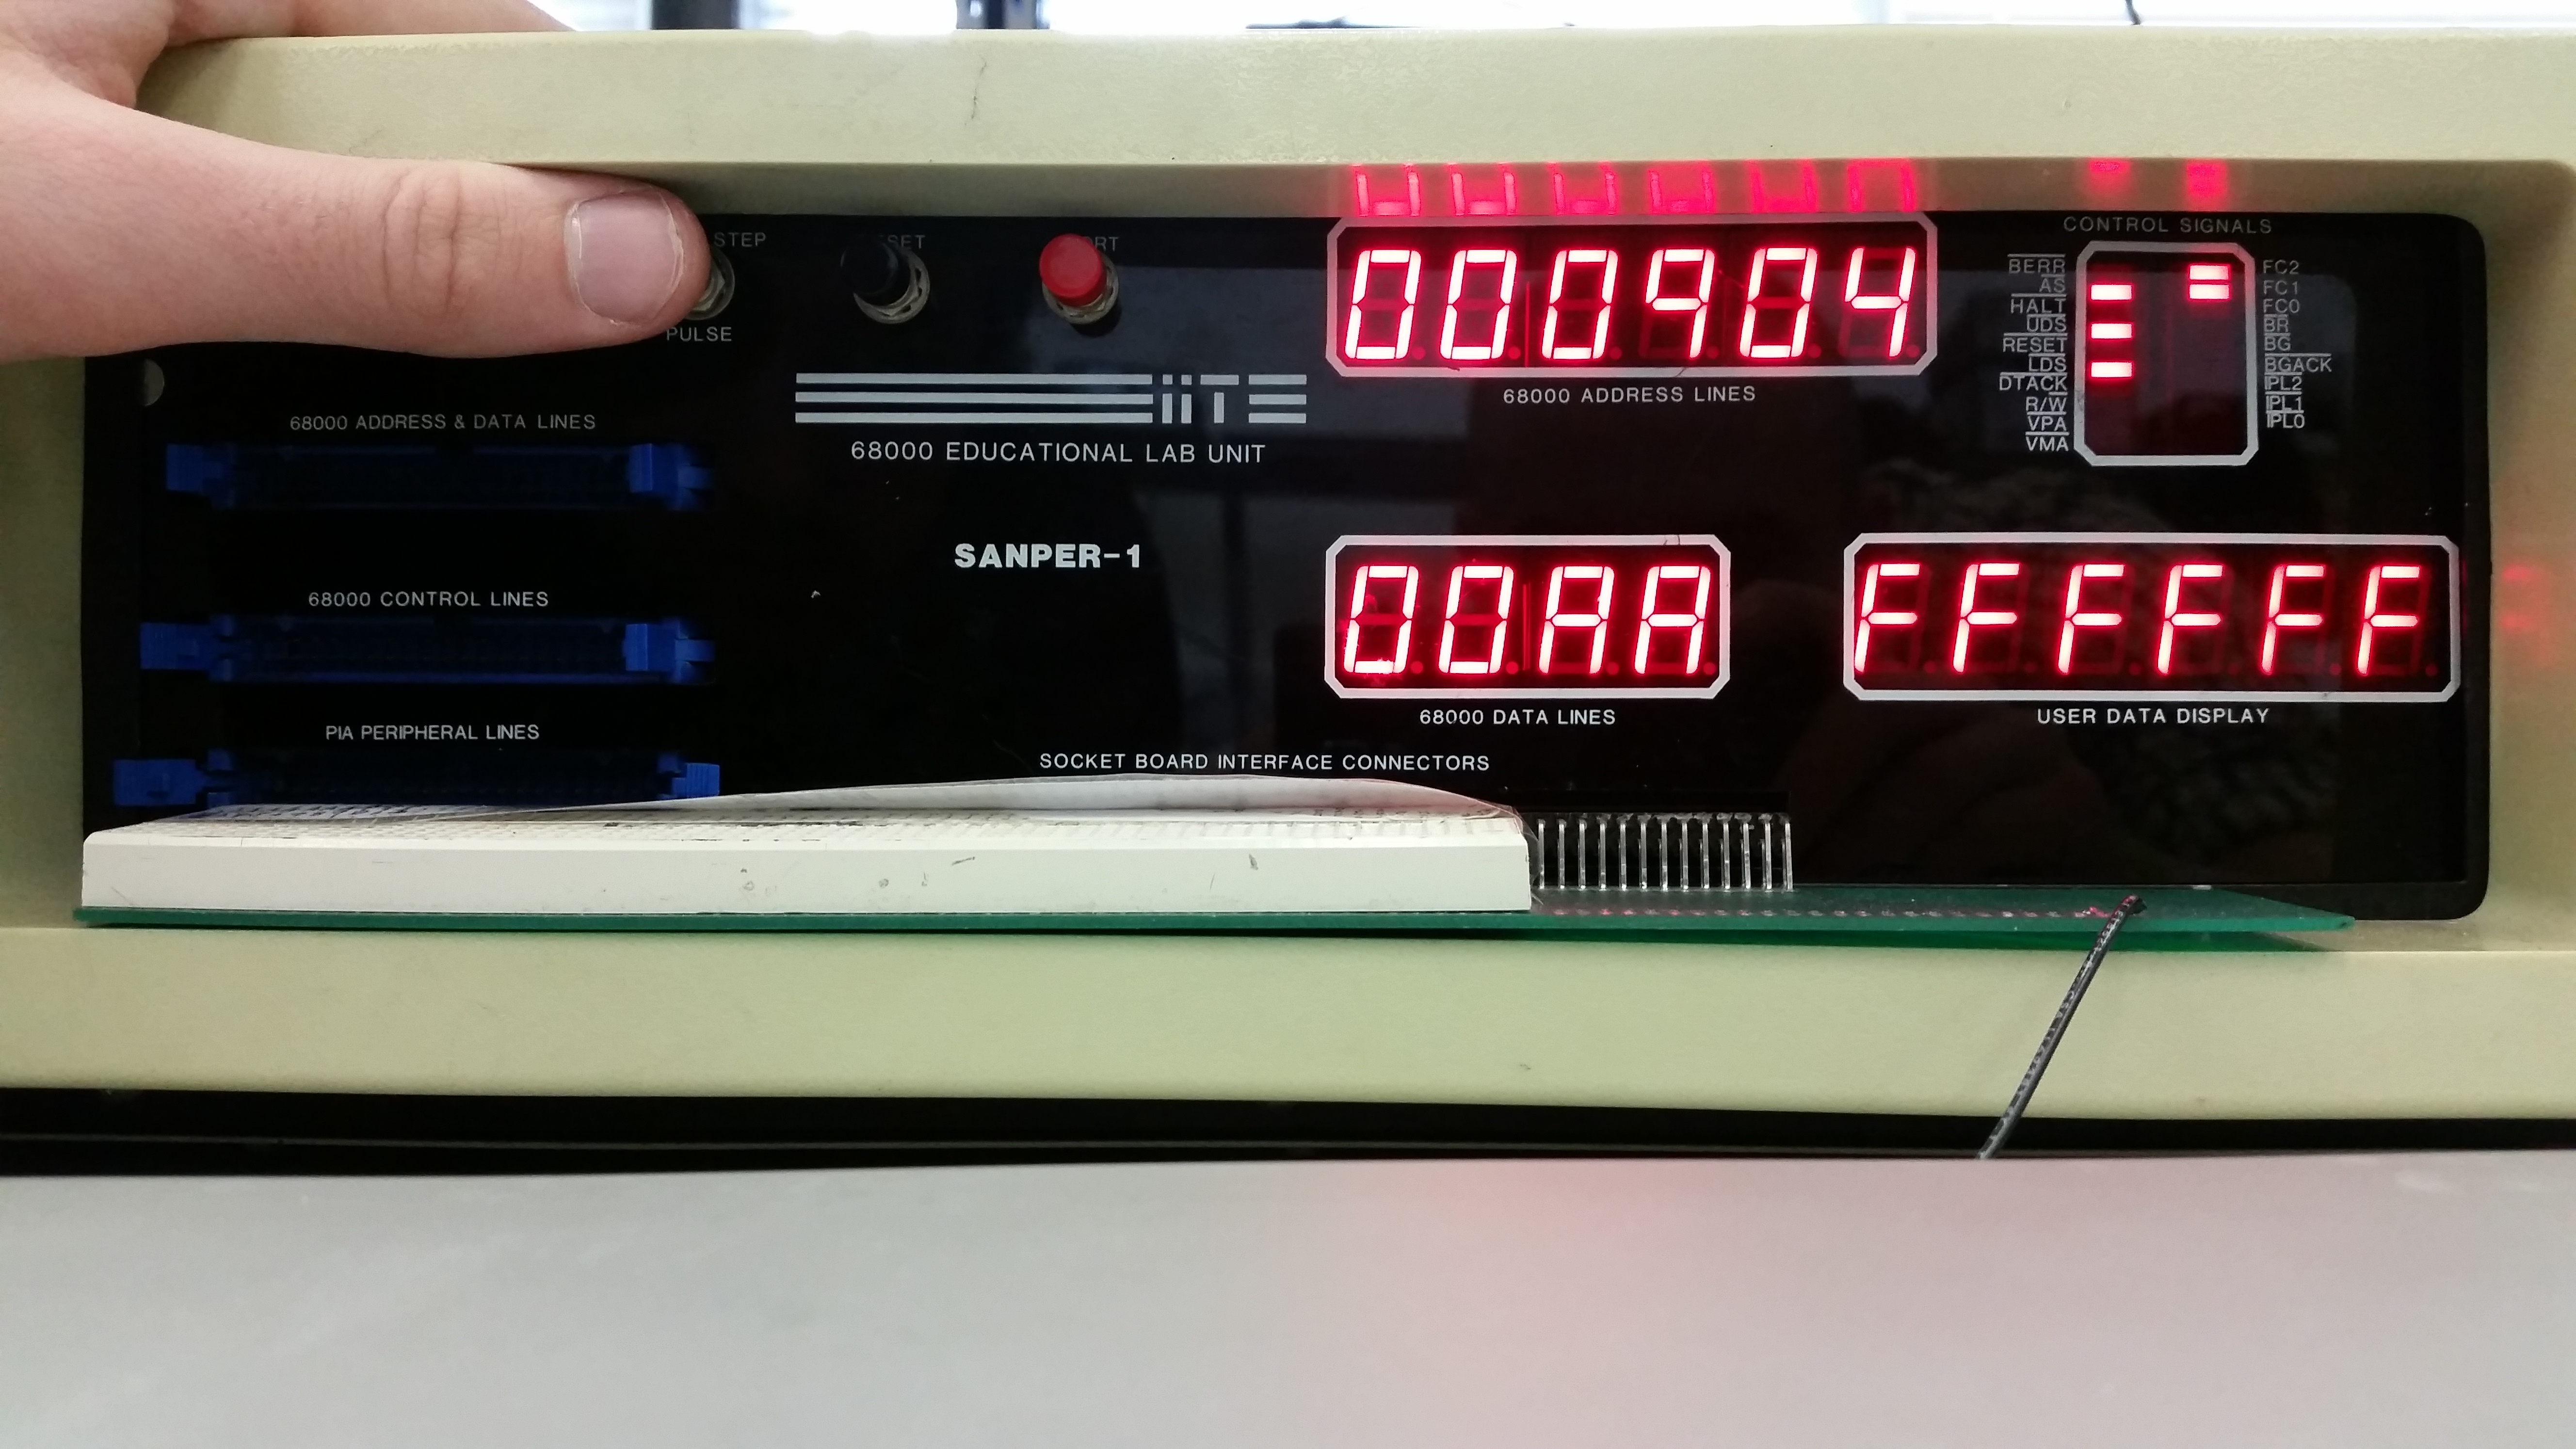
\includegraphics[width=1\linewidth]{Lab1/20150120_094140}
\end{center}
\begin{center}
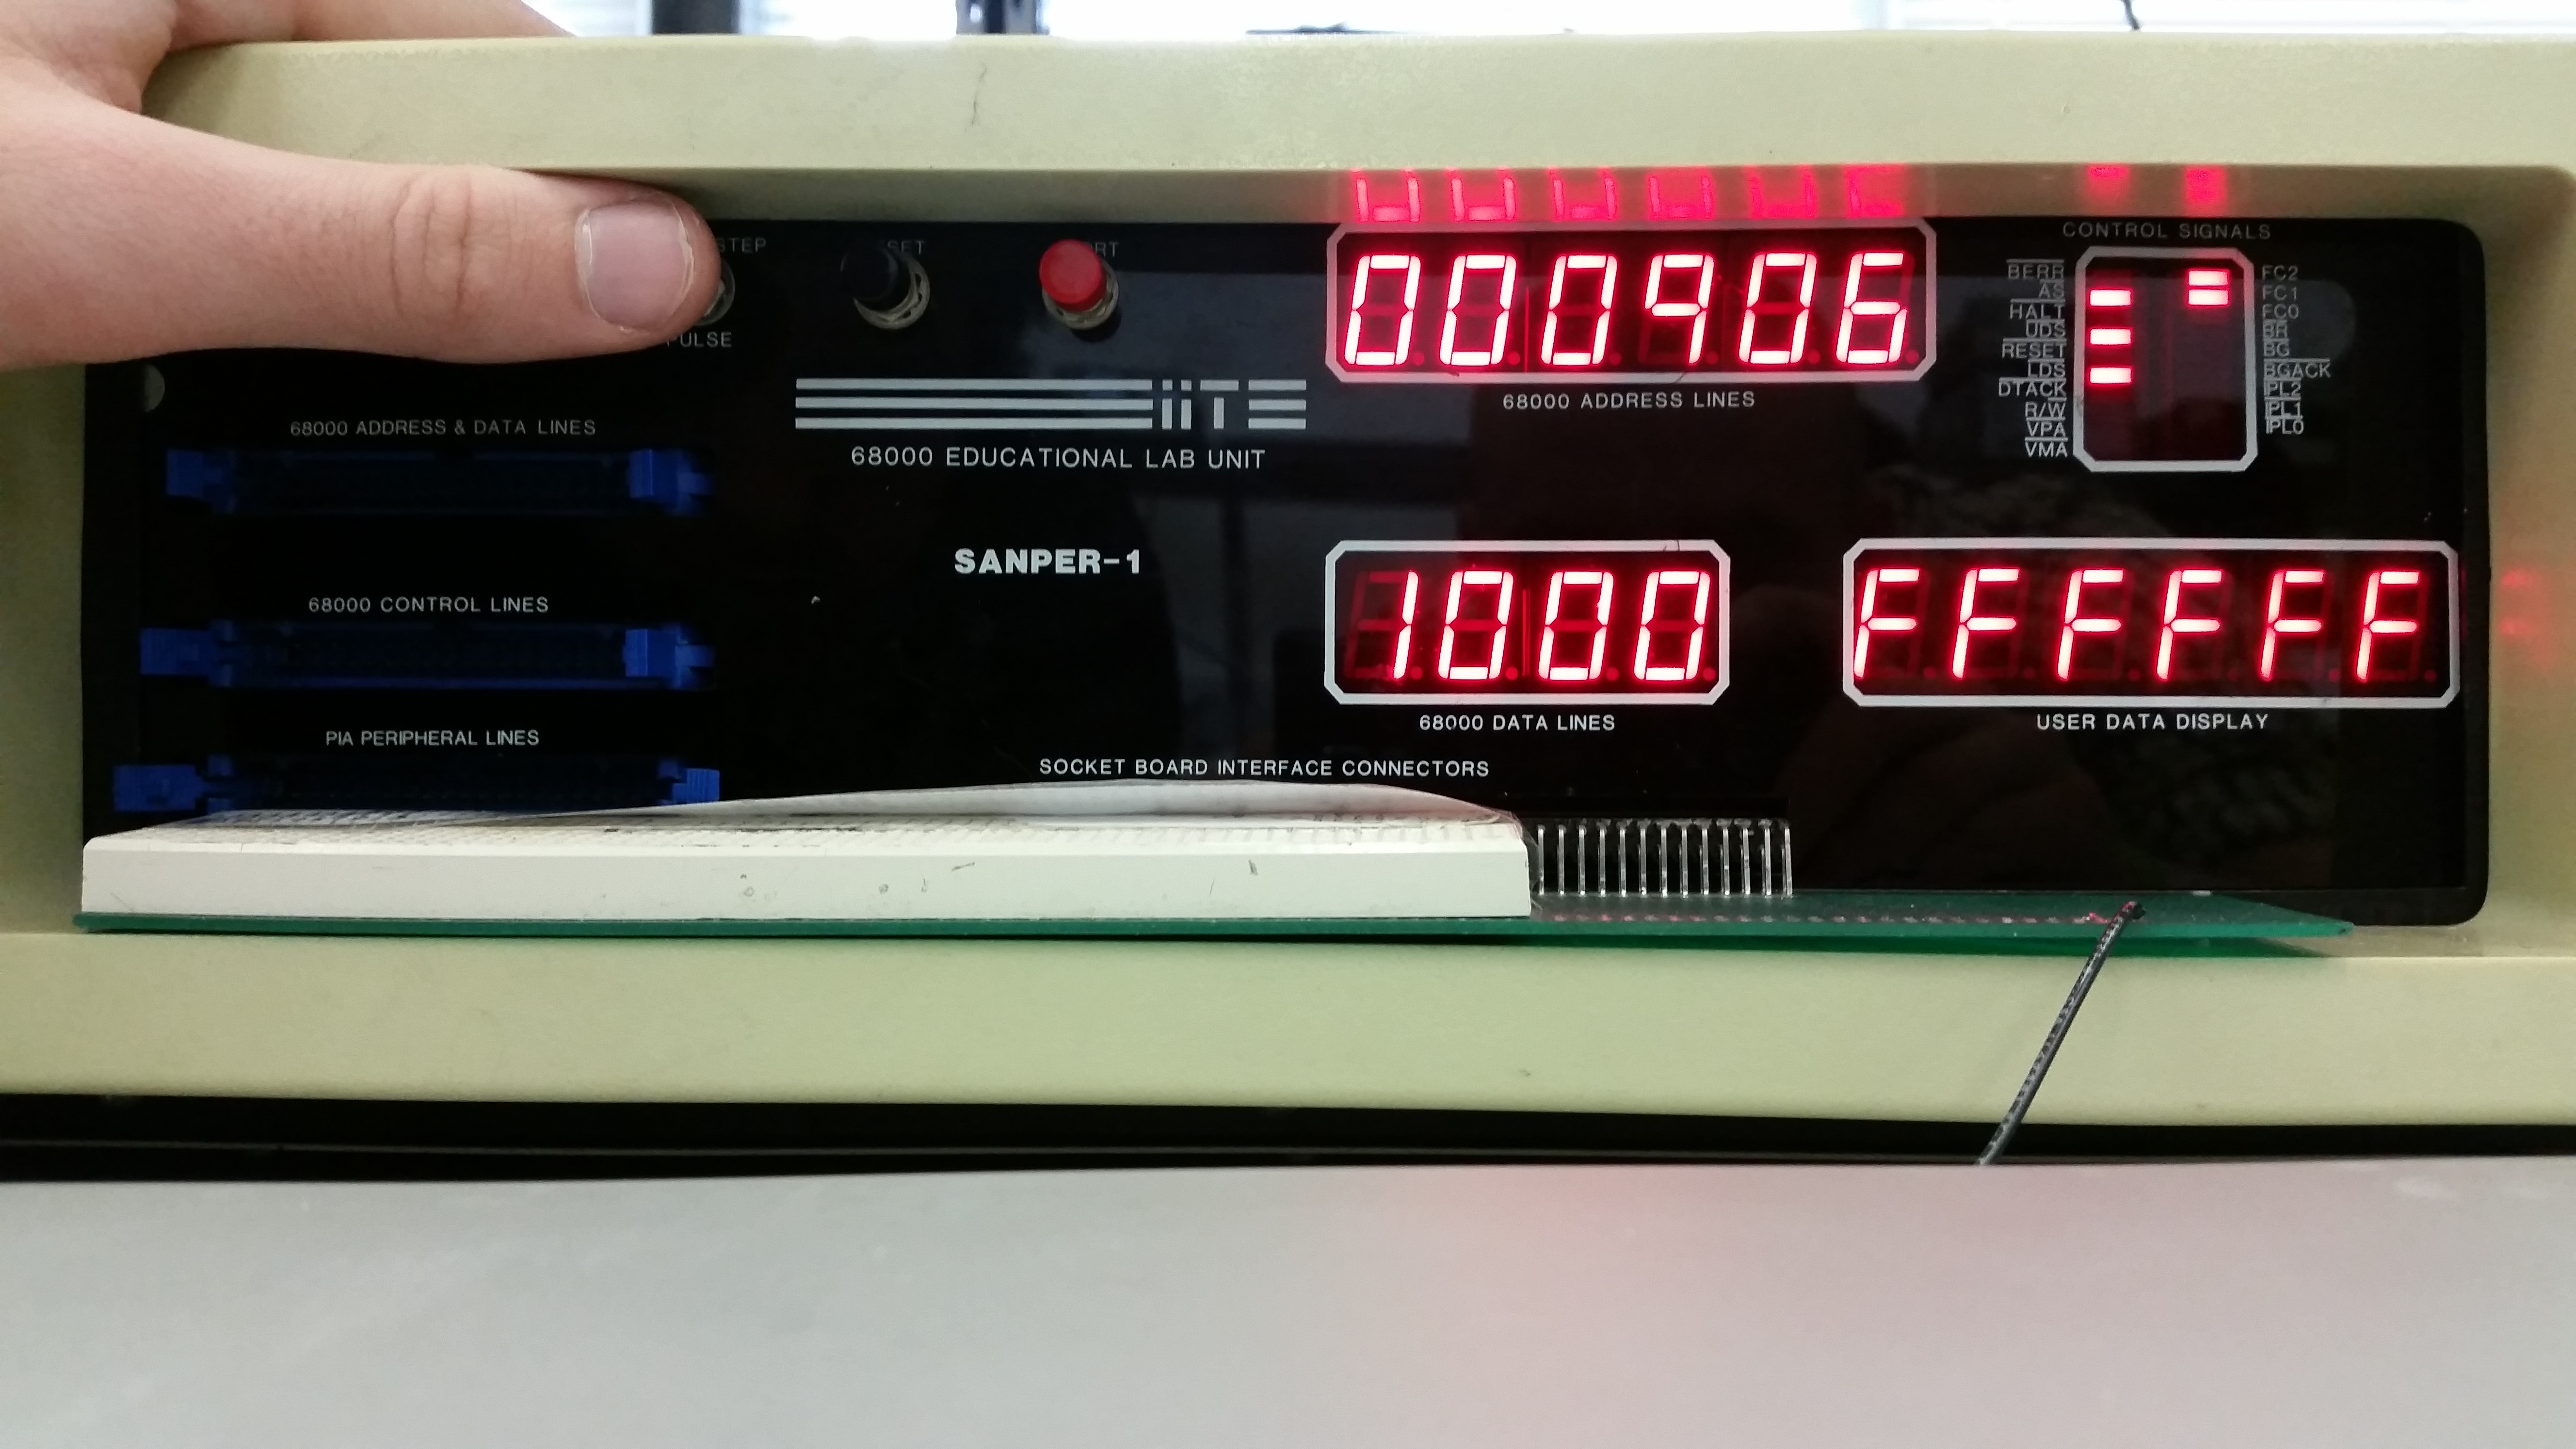
\includegraphics[width=1\linewidth]{Lab1/20150120_094142}
\end{center}
\begin{center}
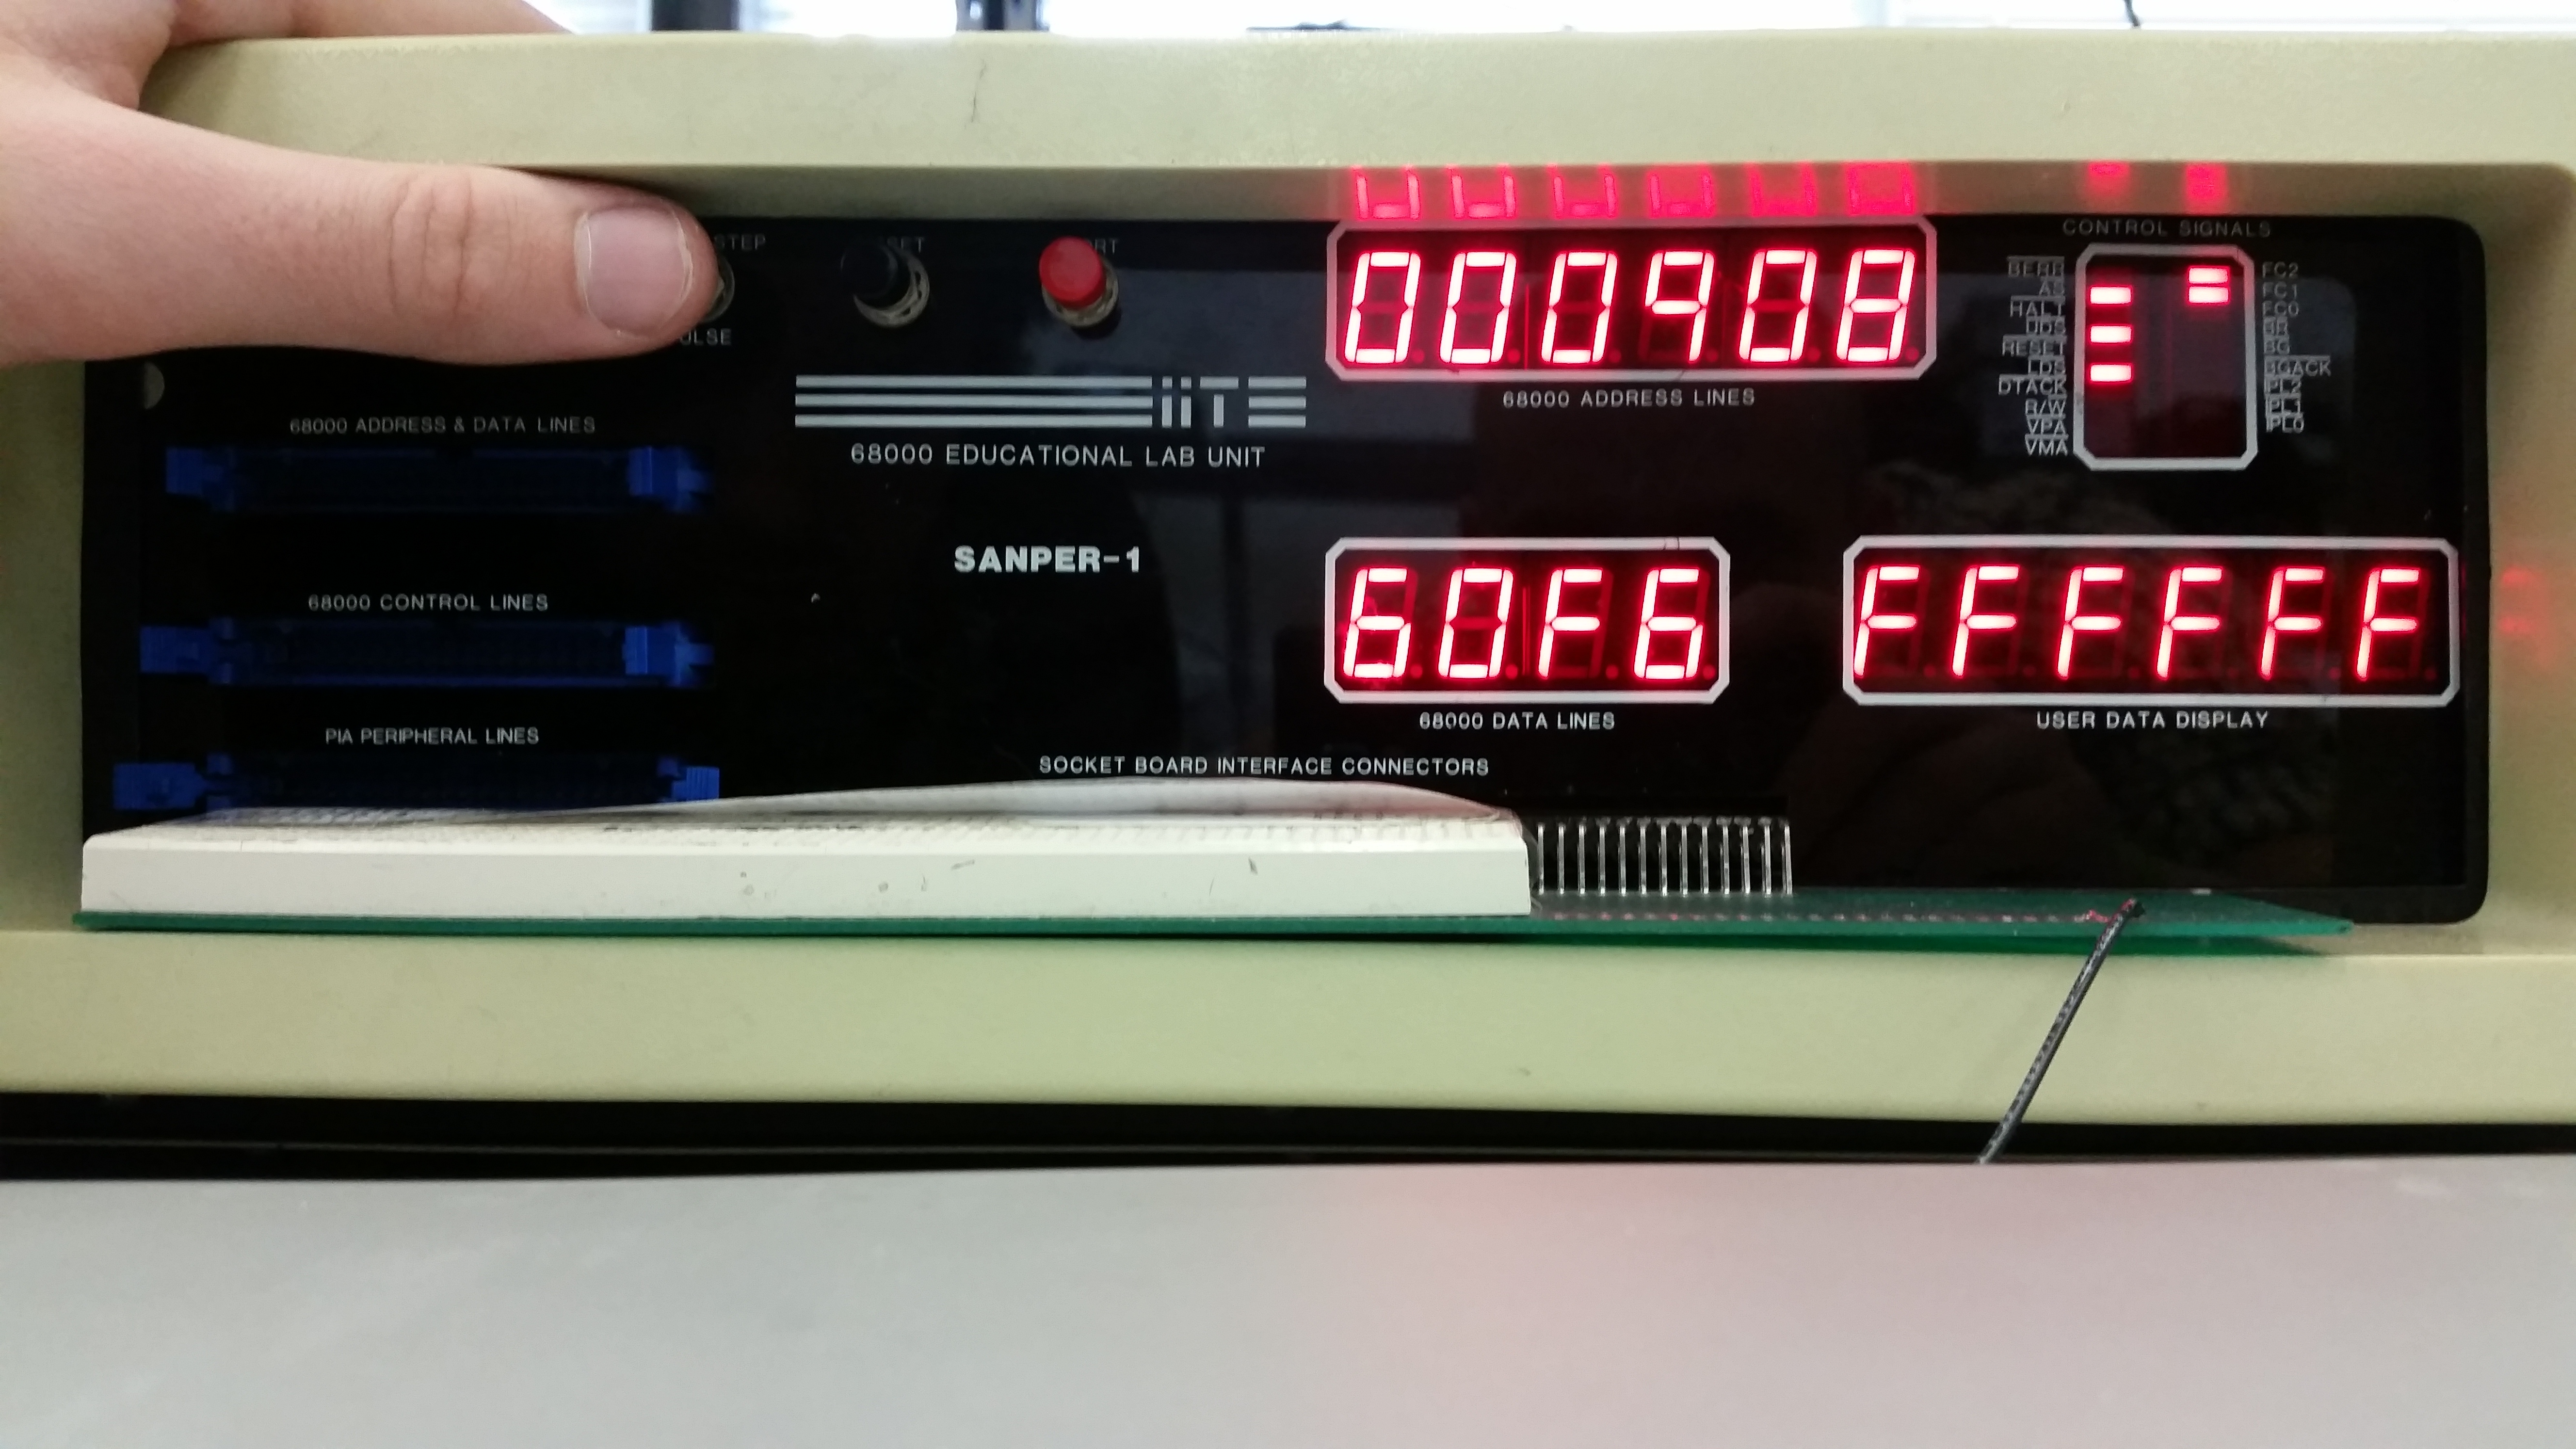
\includegraphics[width=1\linewidth]{Lab1/20150120_094143}
\end{center}
\begin{center}
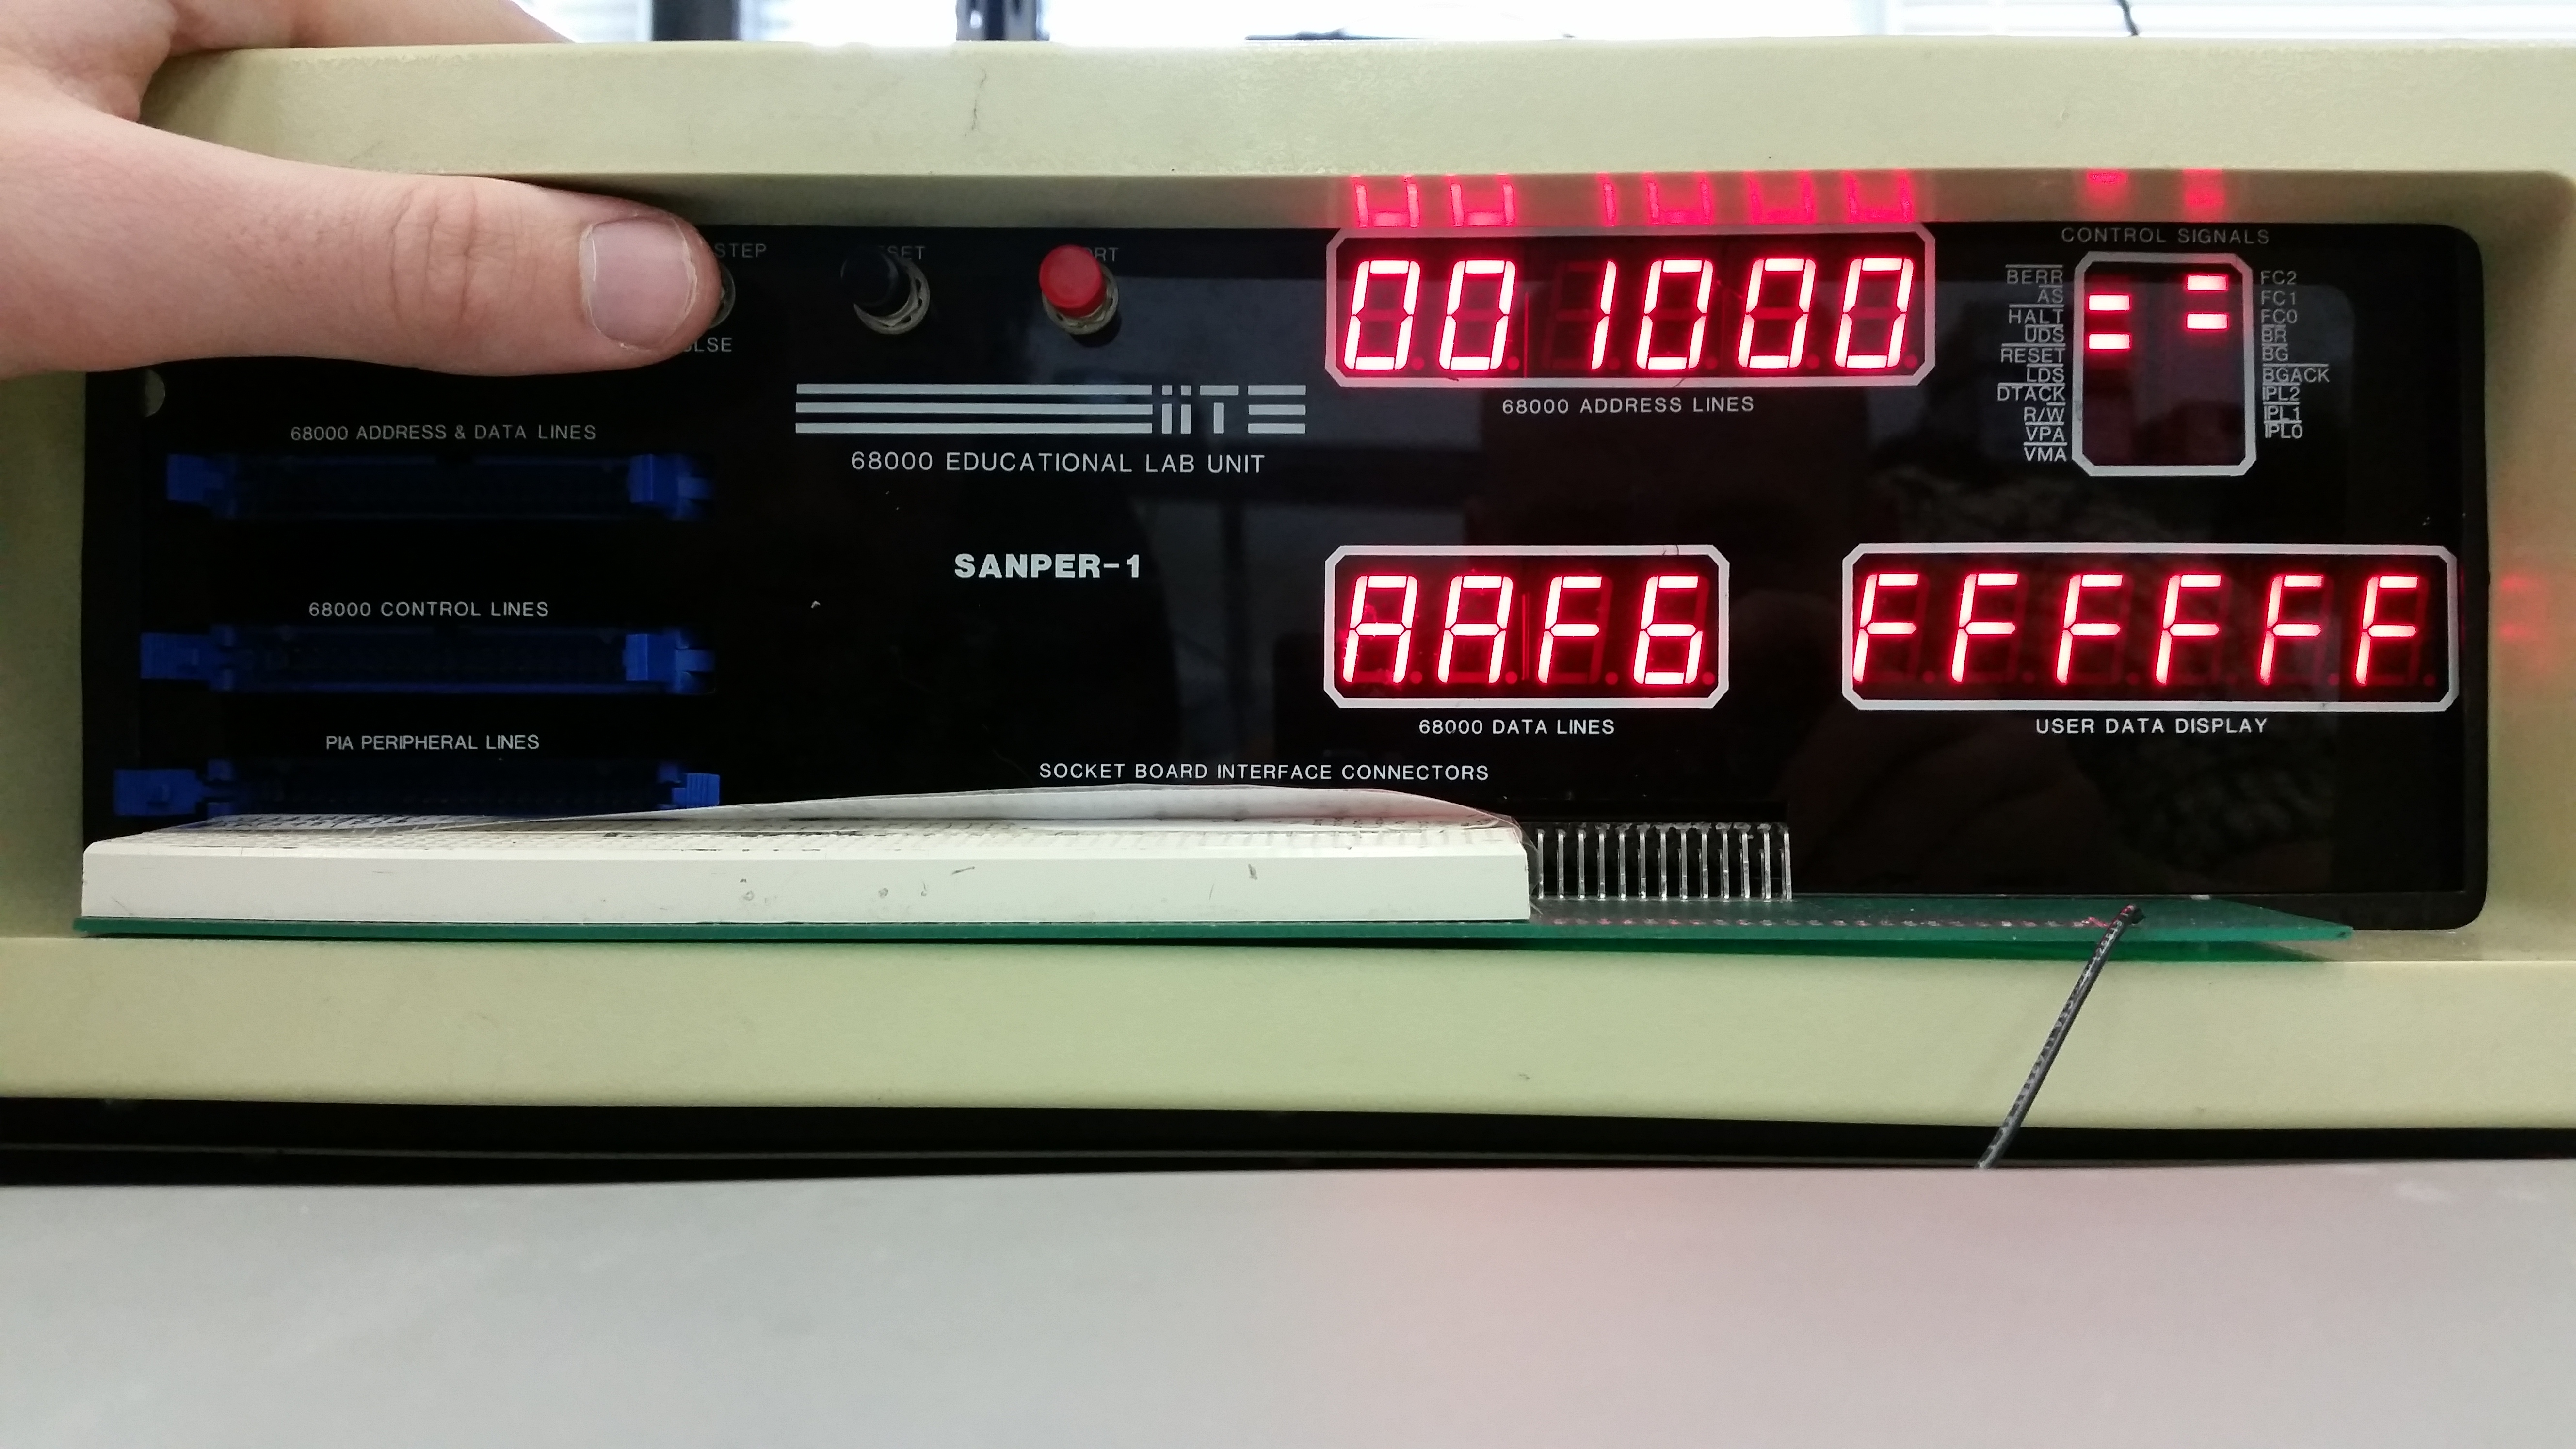
\includegraphics[width=1\linewidth]{Lab1/20150120_094147}
\end{center}
\begin{center}
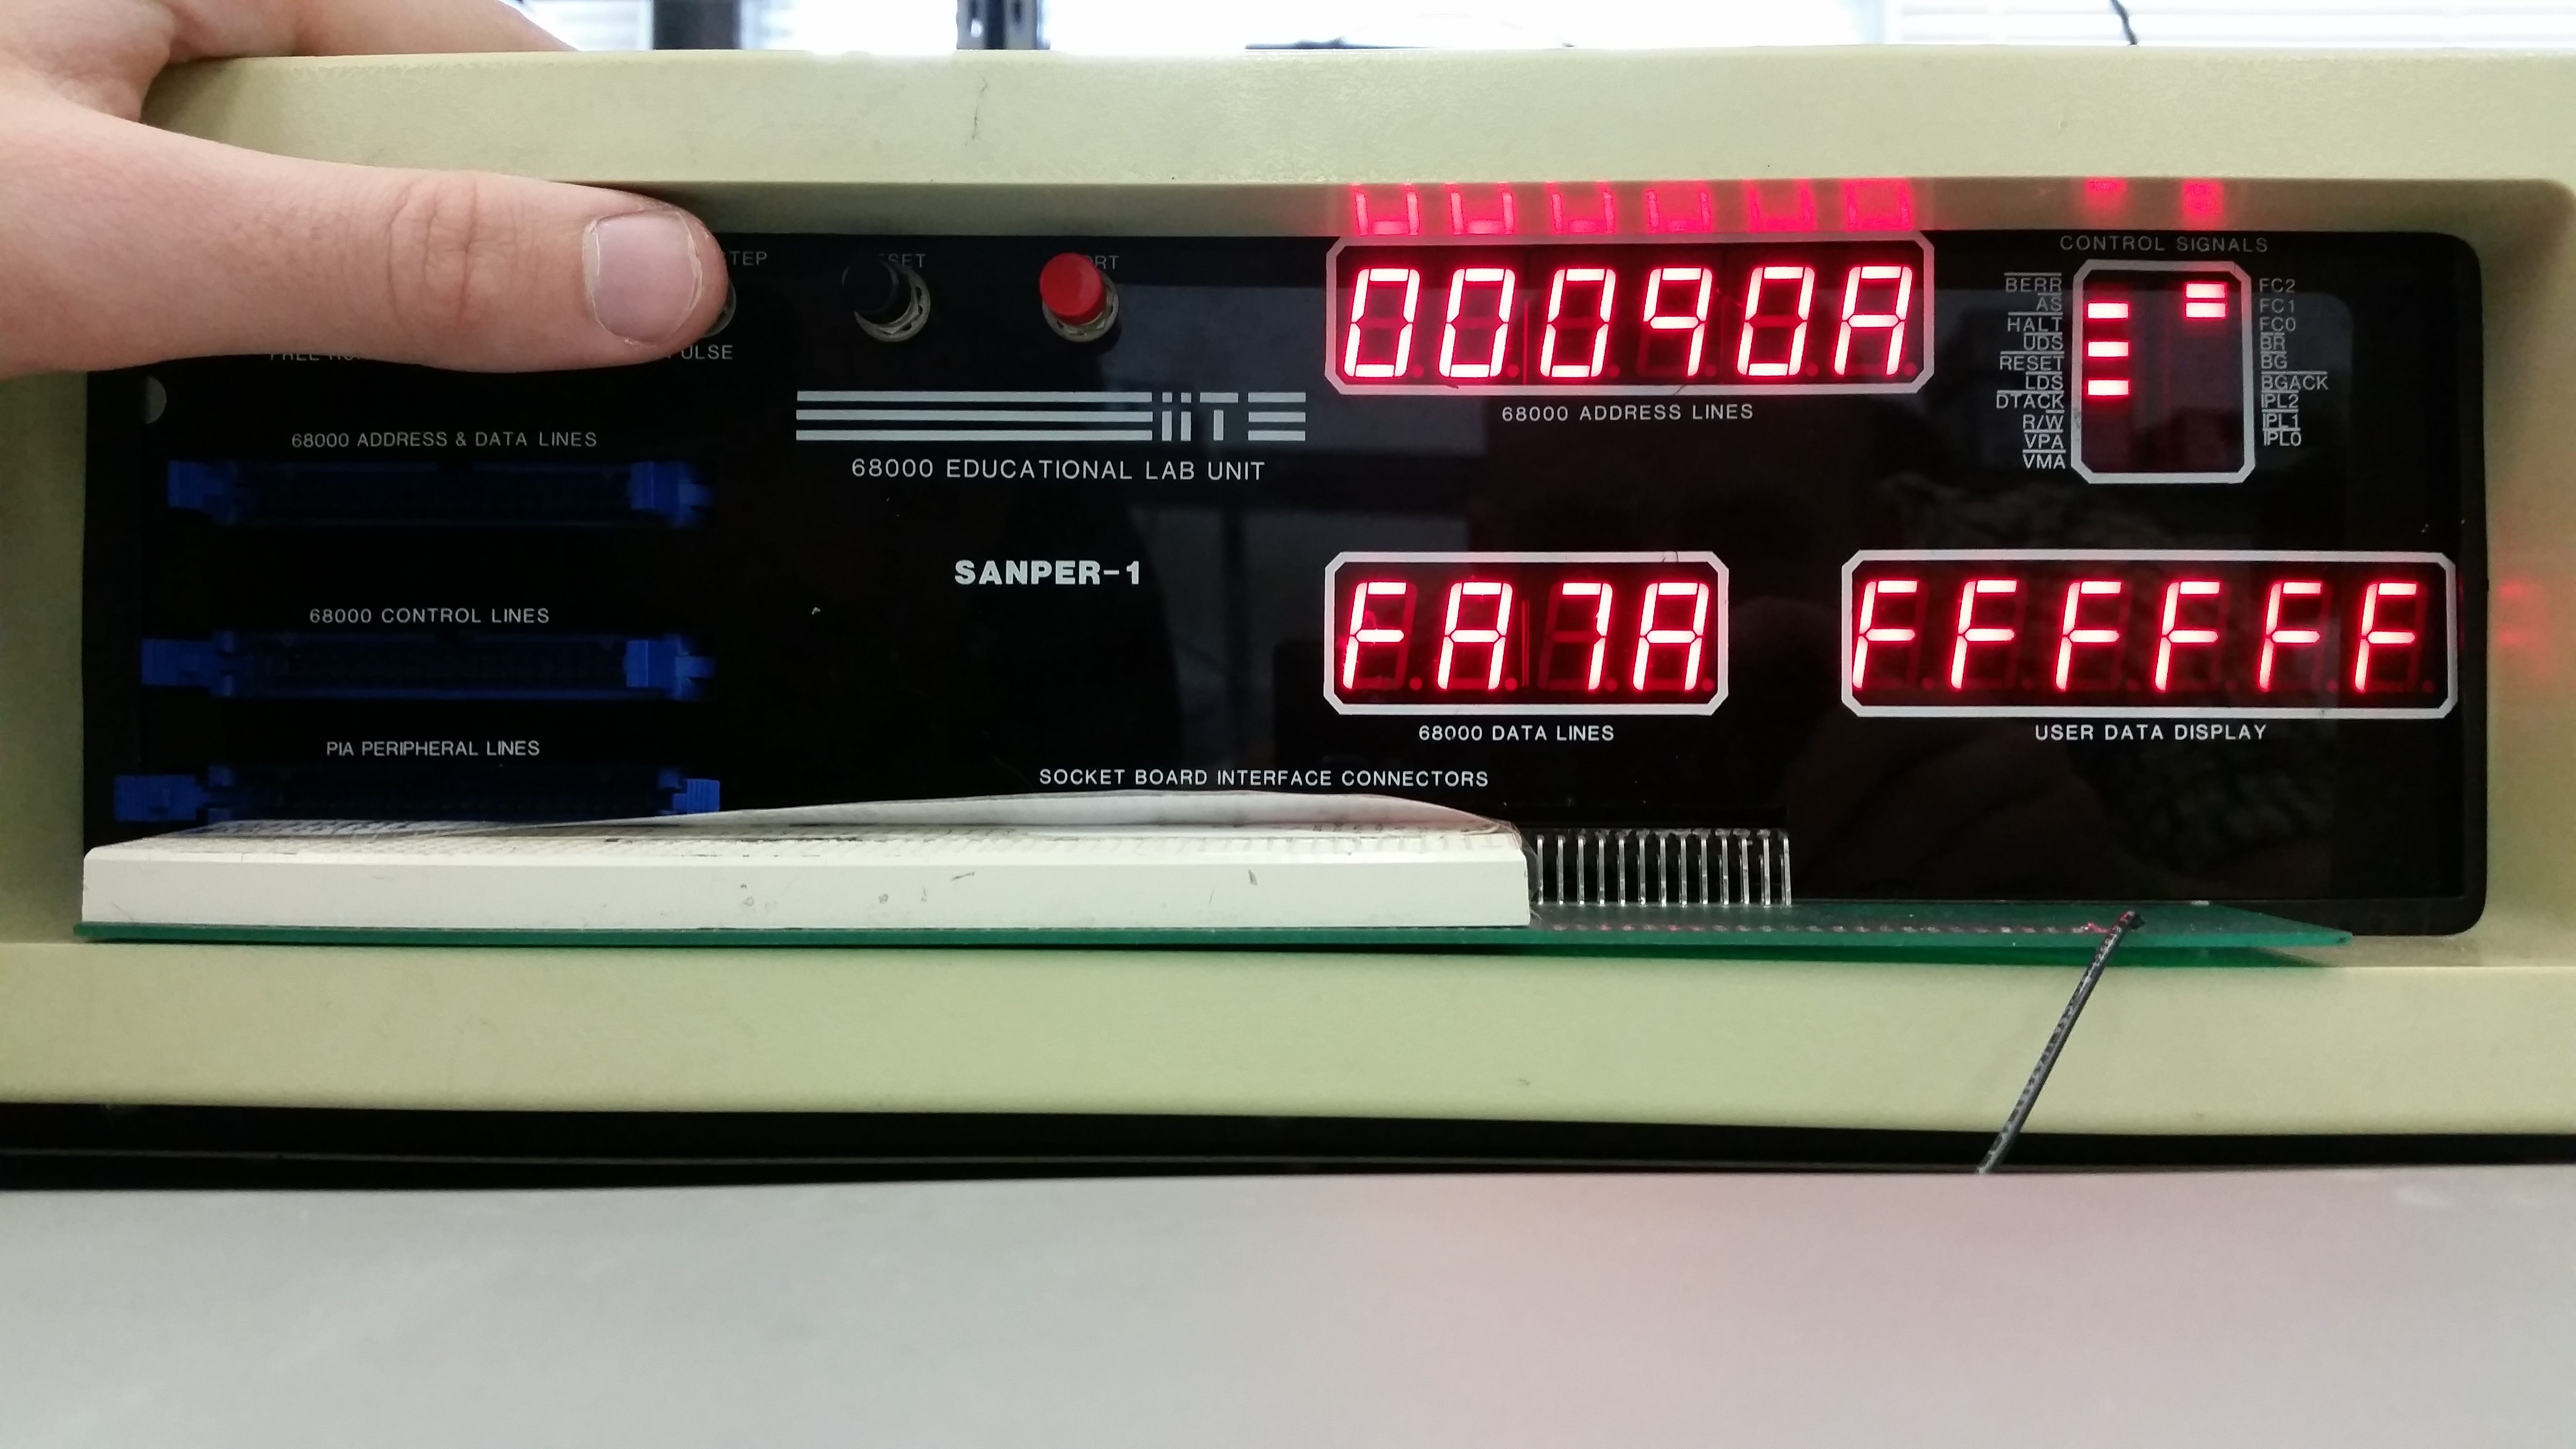
\includegraphics[width=1\linewidth]{Lab1/20150120_094151}
\end{center}
\begin{center}
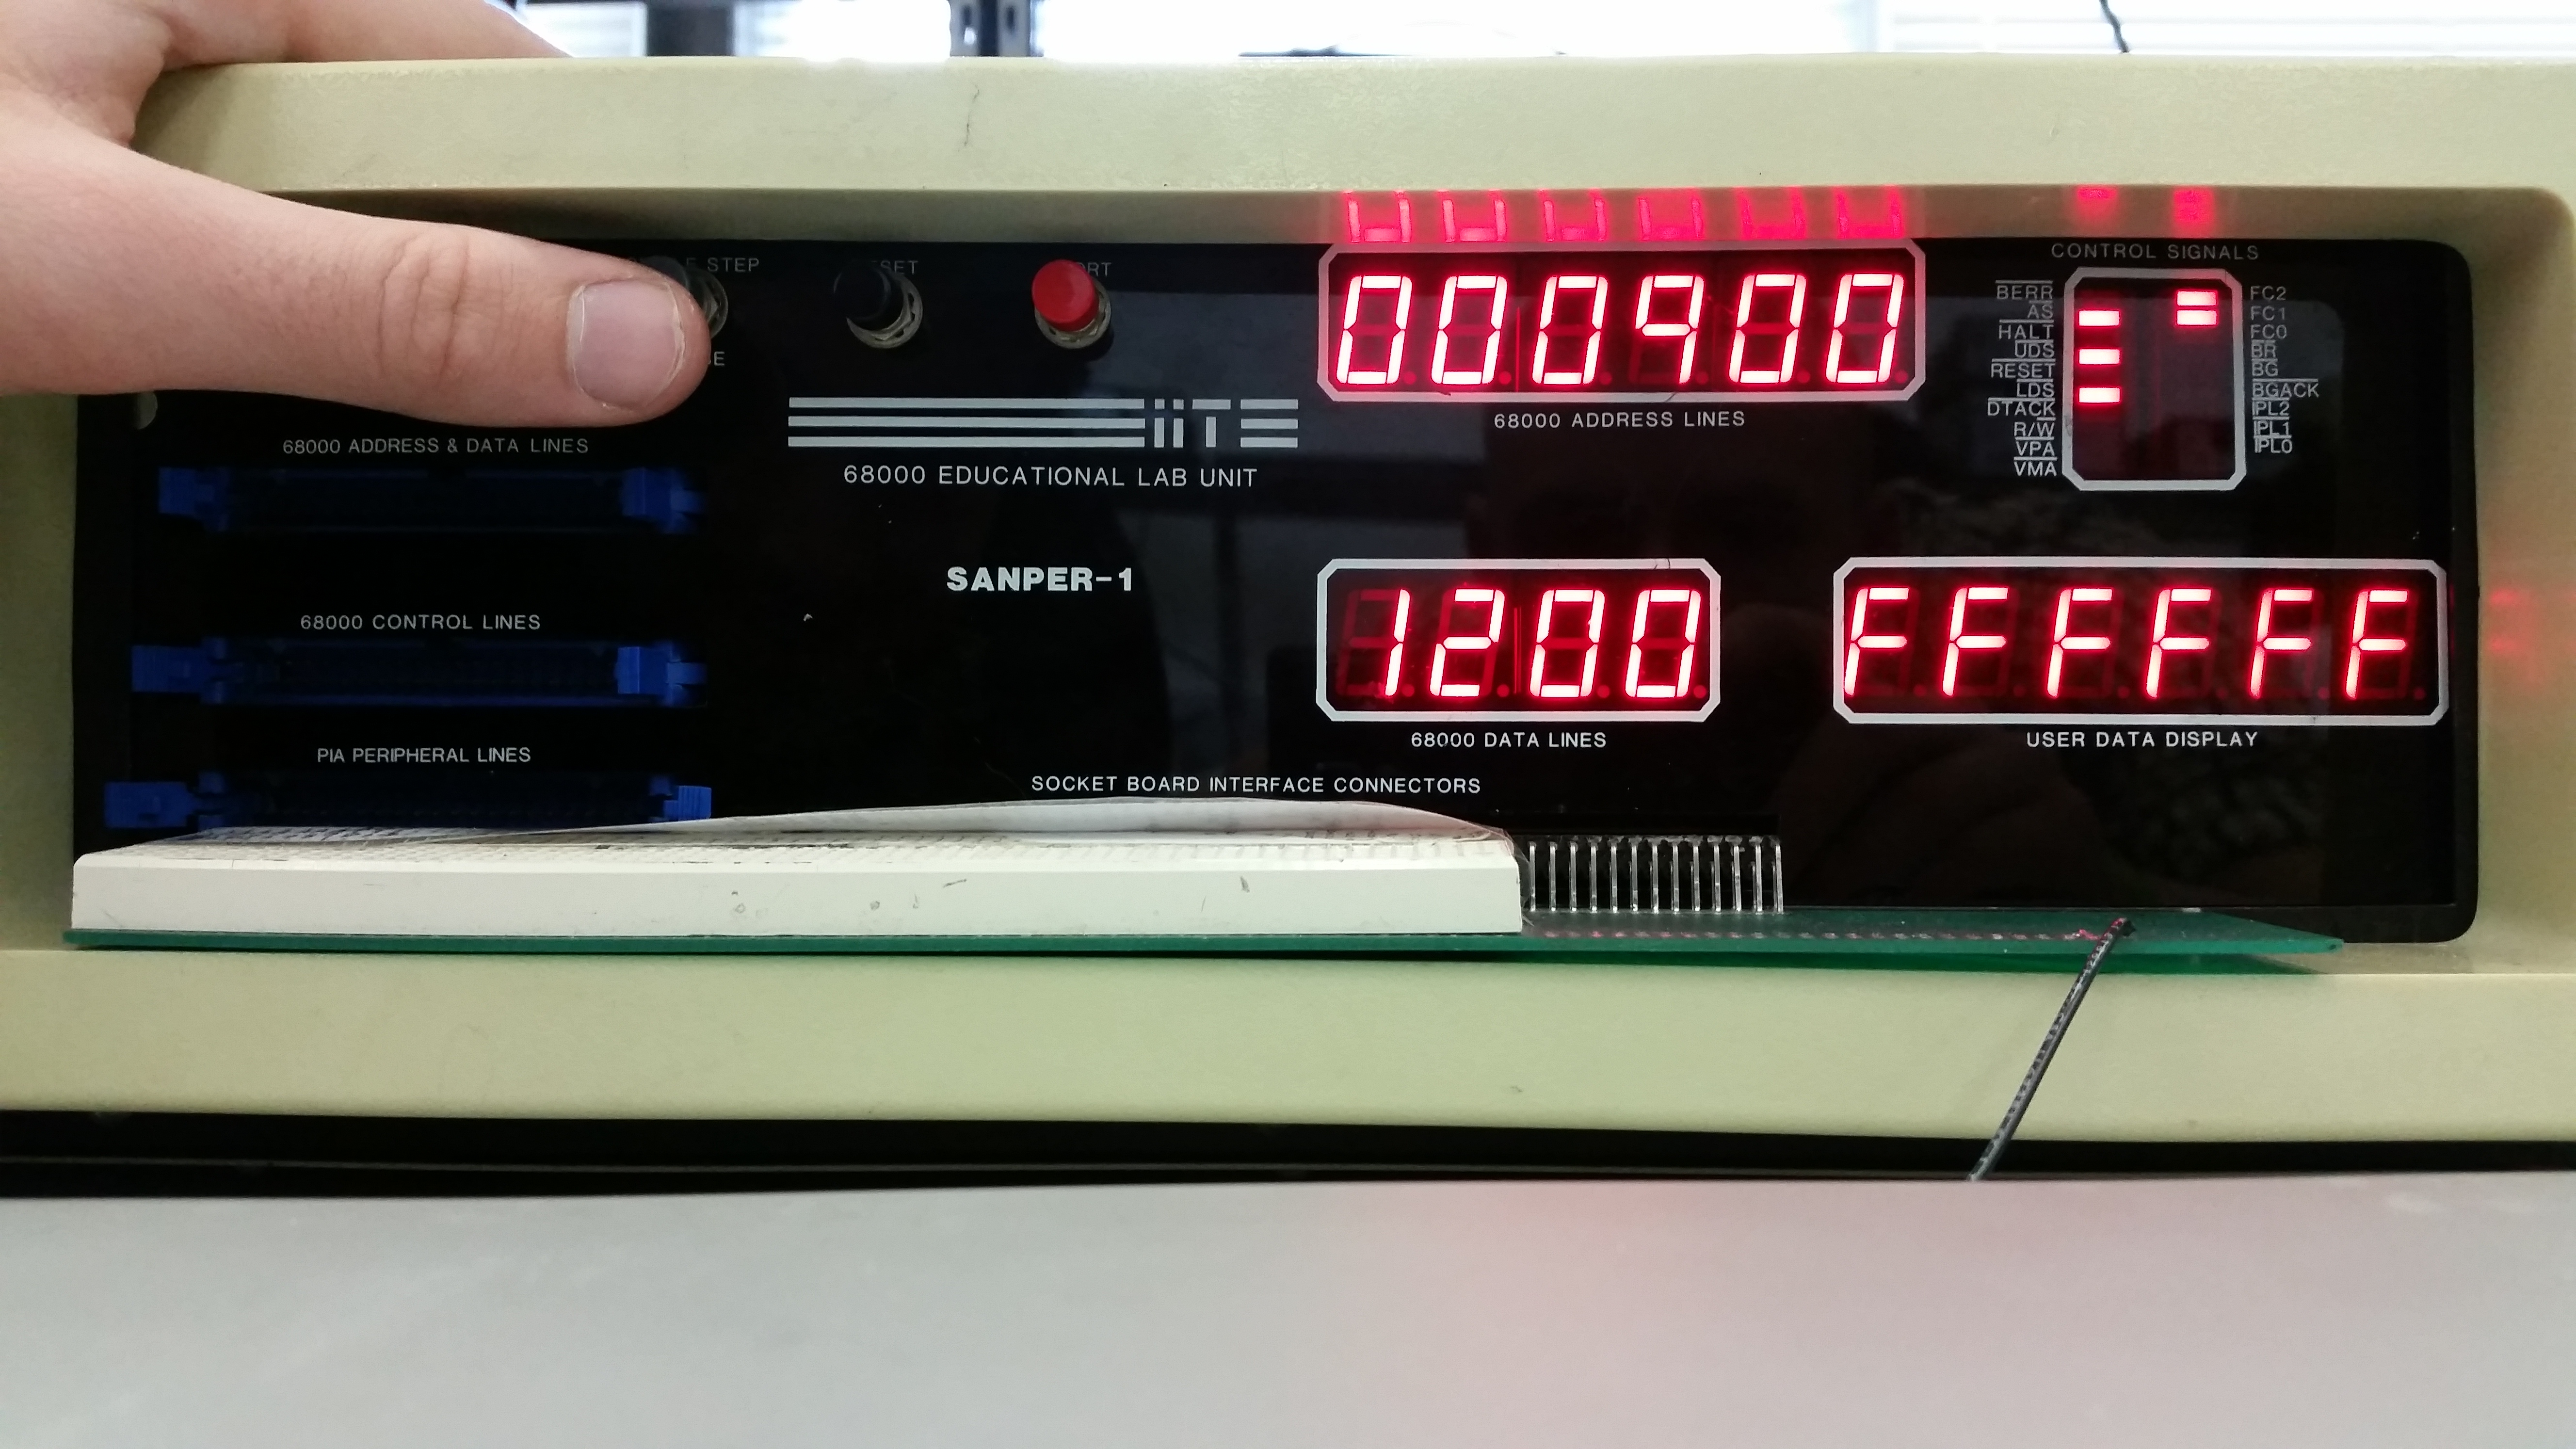
\includegraphics[width=1\linewidth]{Lab1/20150120_094154}
\end{center}
\subsubsection{Program 3}
\begin{center}
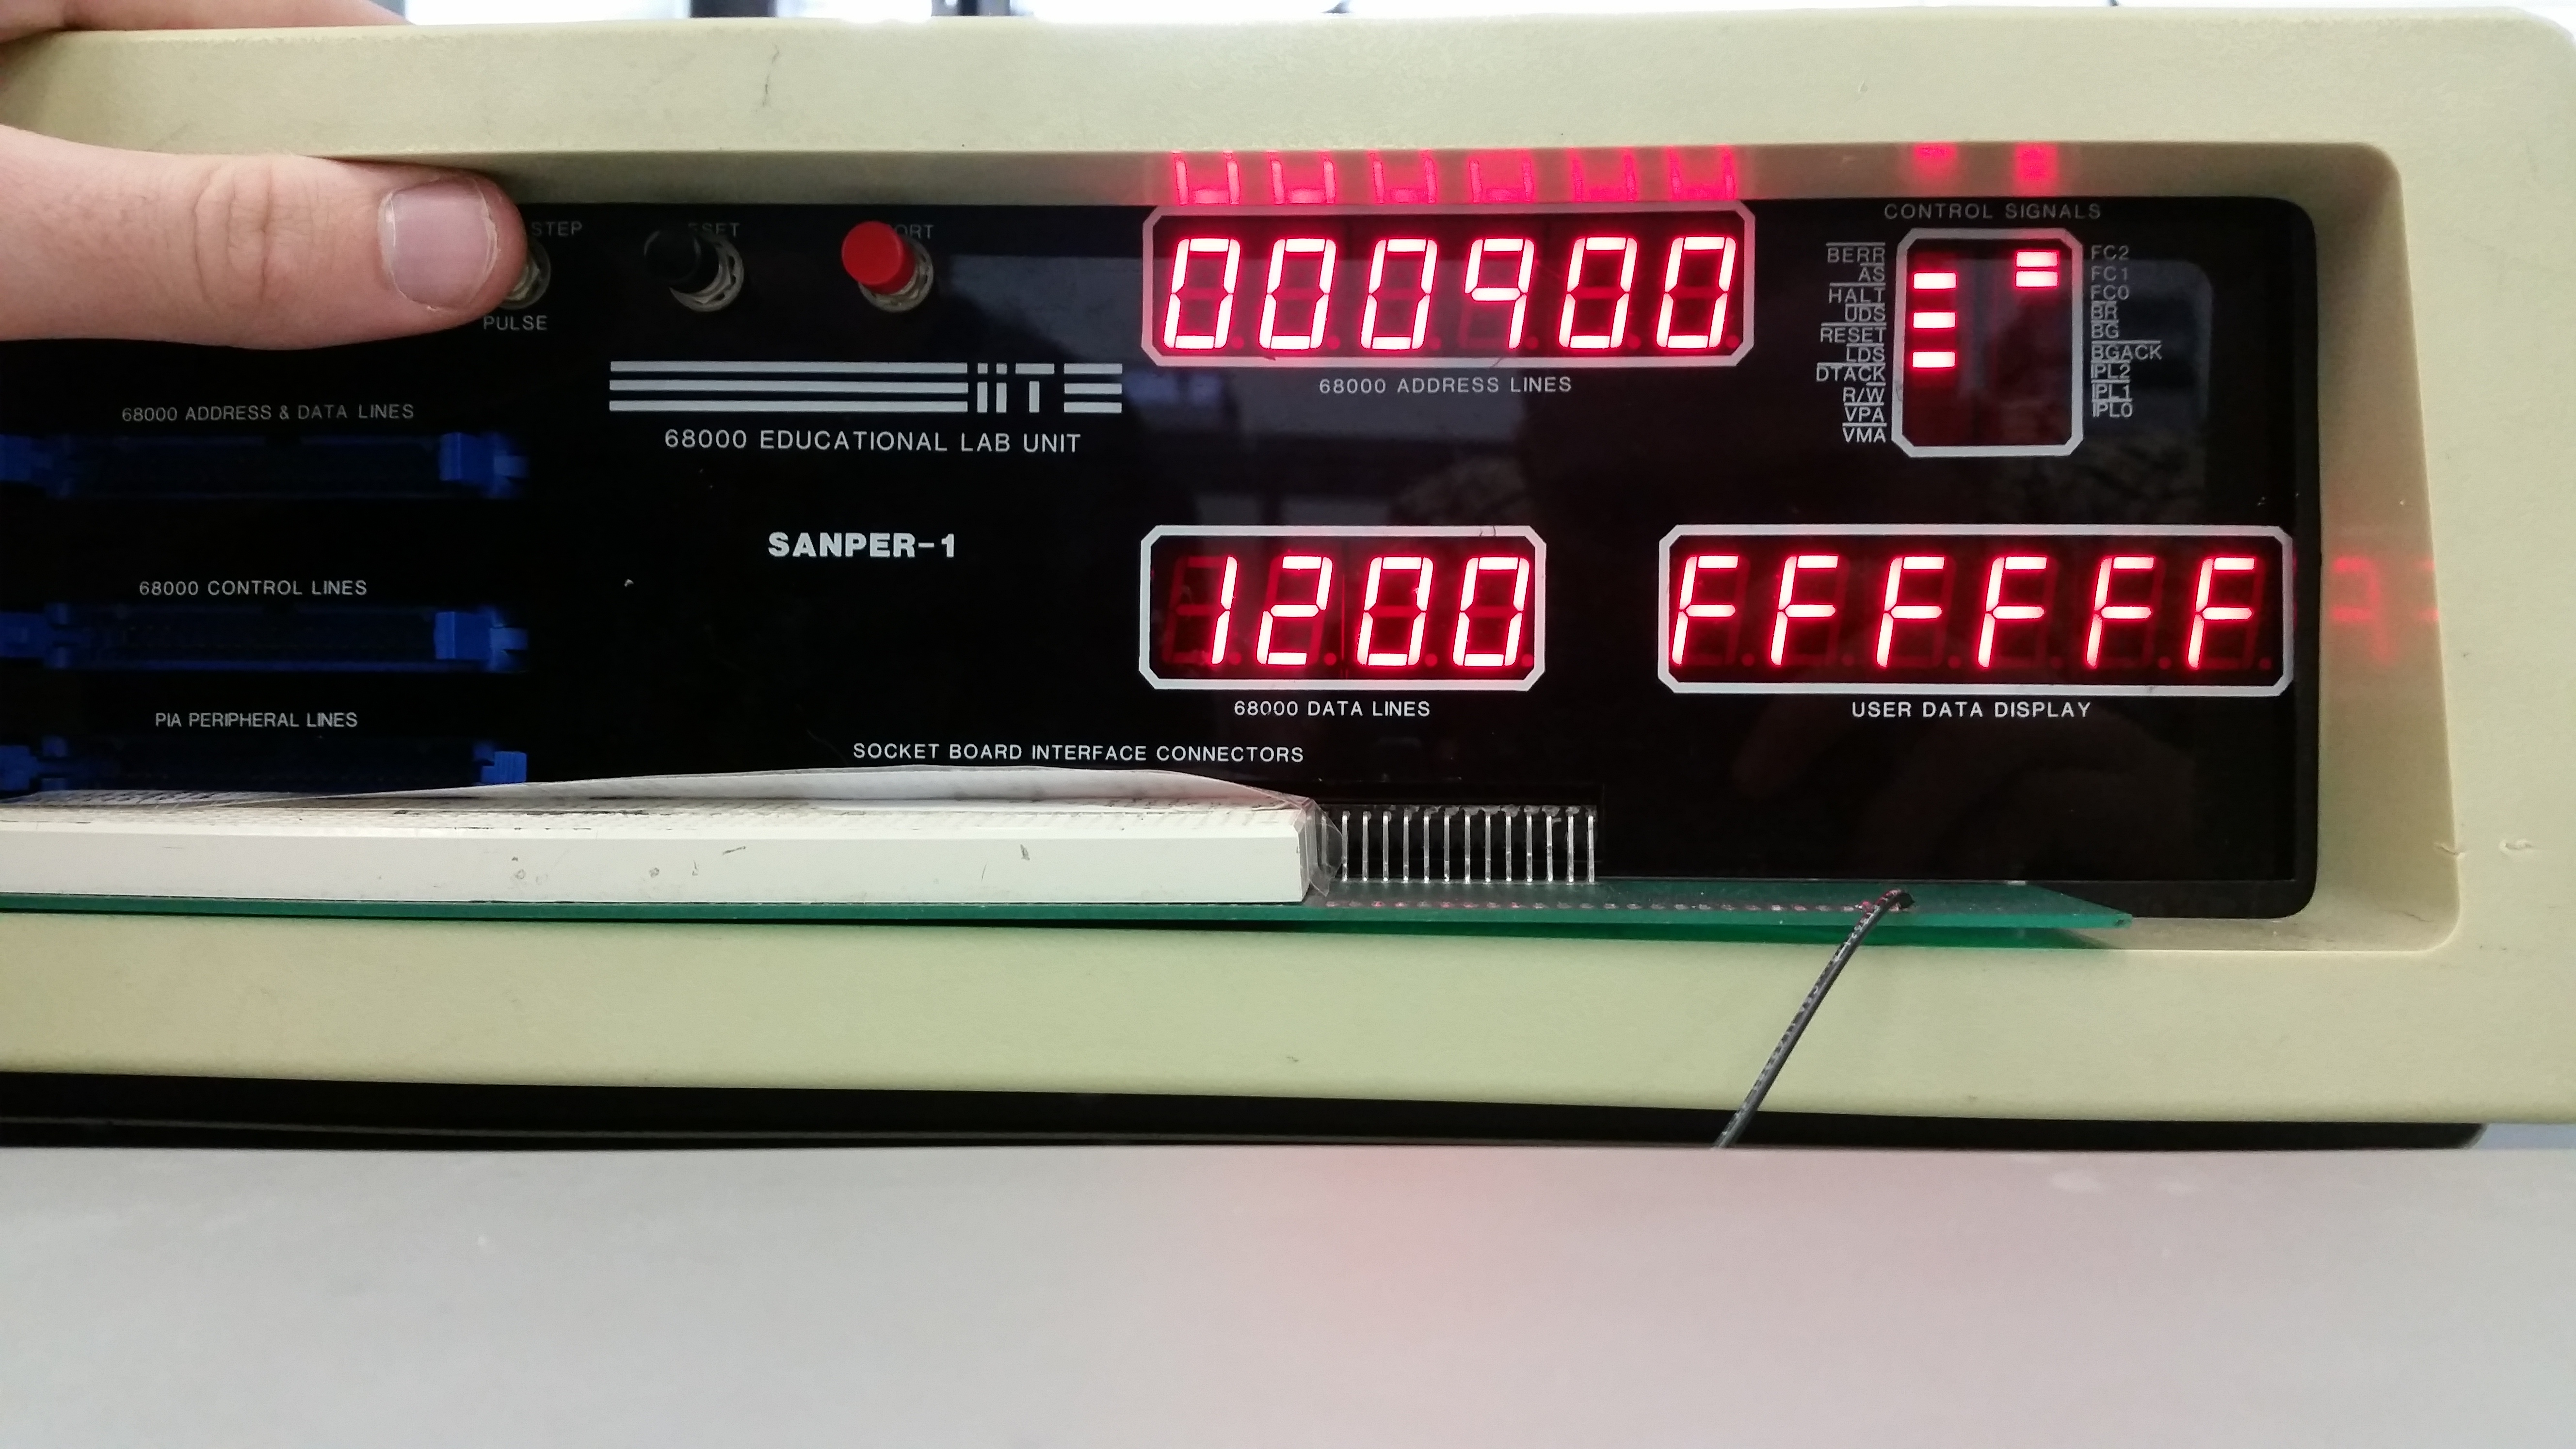
\includegraphics[width=1\linewidth]{Lab1/20150120_094638}
\end{center}
\begin{center}
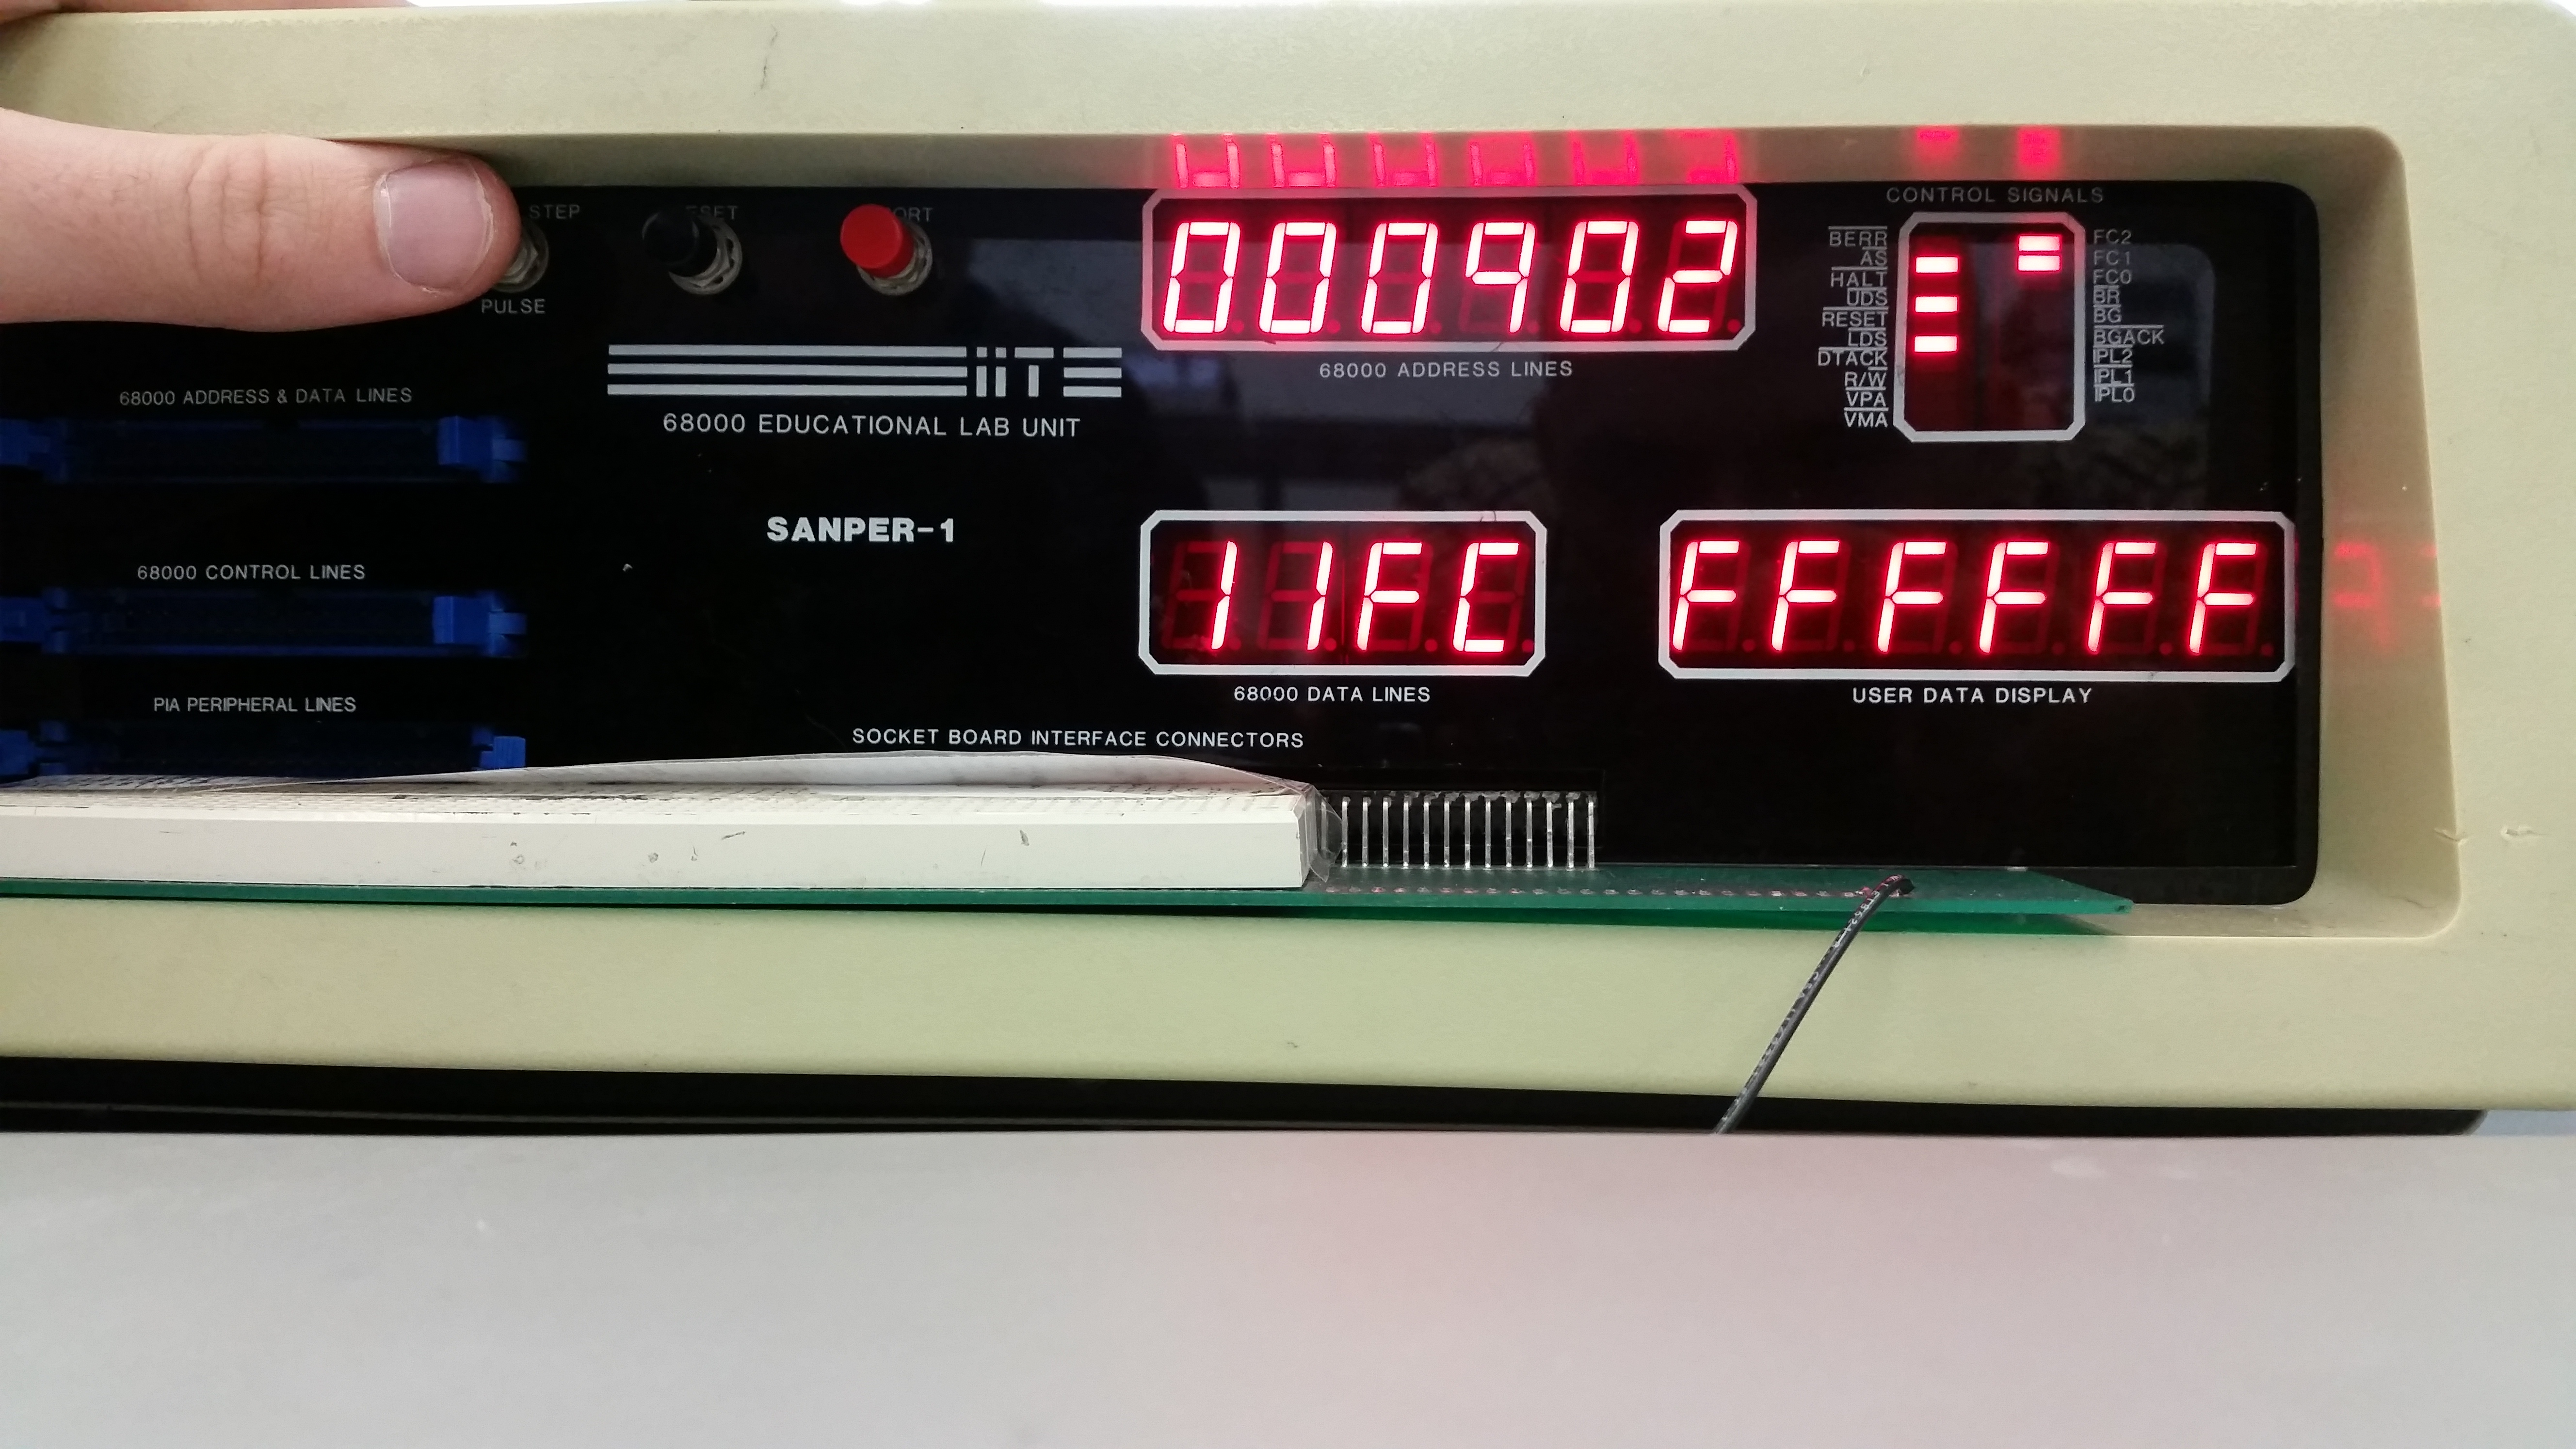
\includegraphics[width=1\linewidth]{Lab1/20150120_094640}
\end{center}
\begin{center}
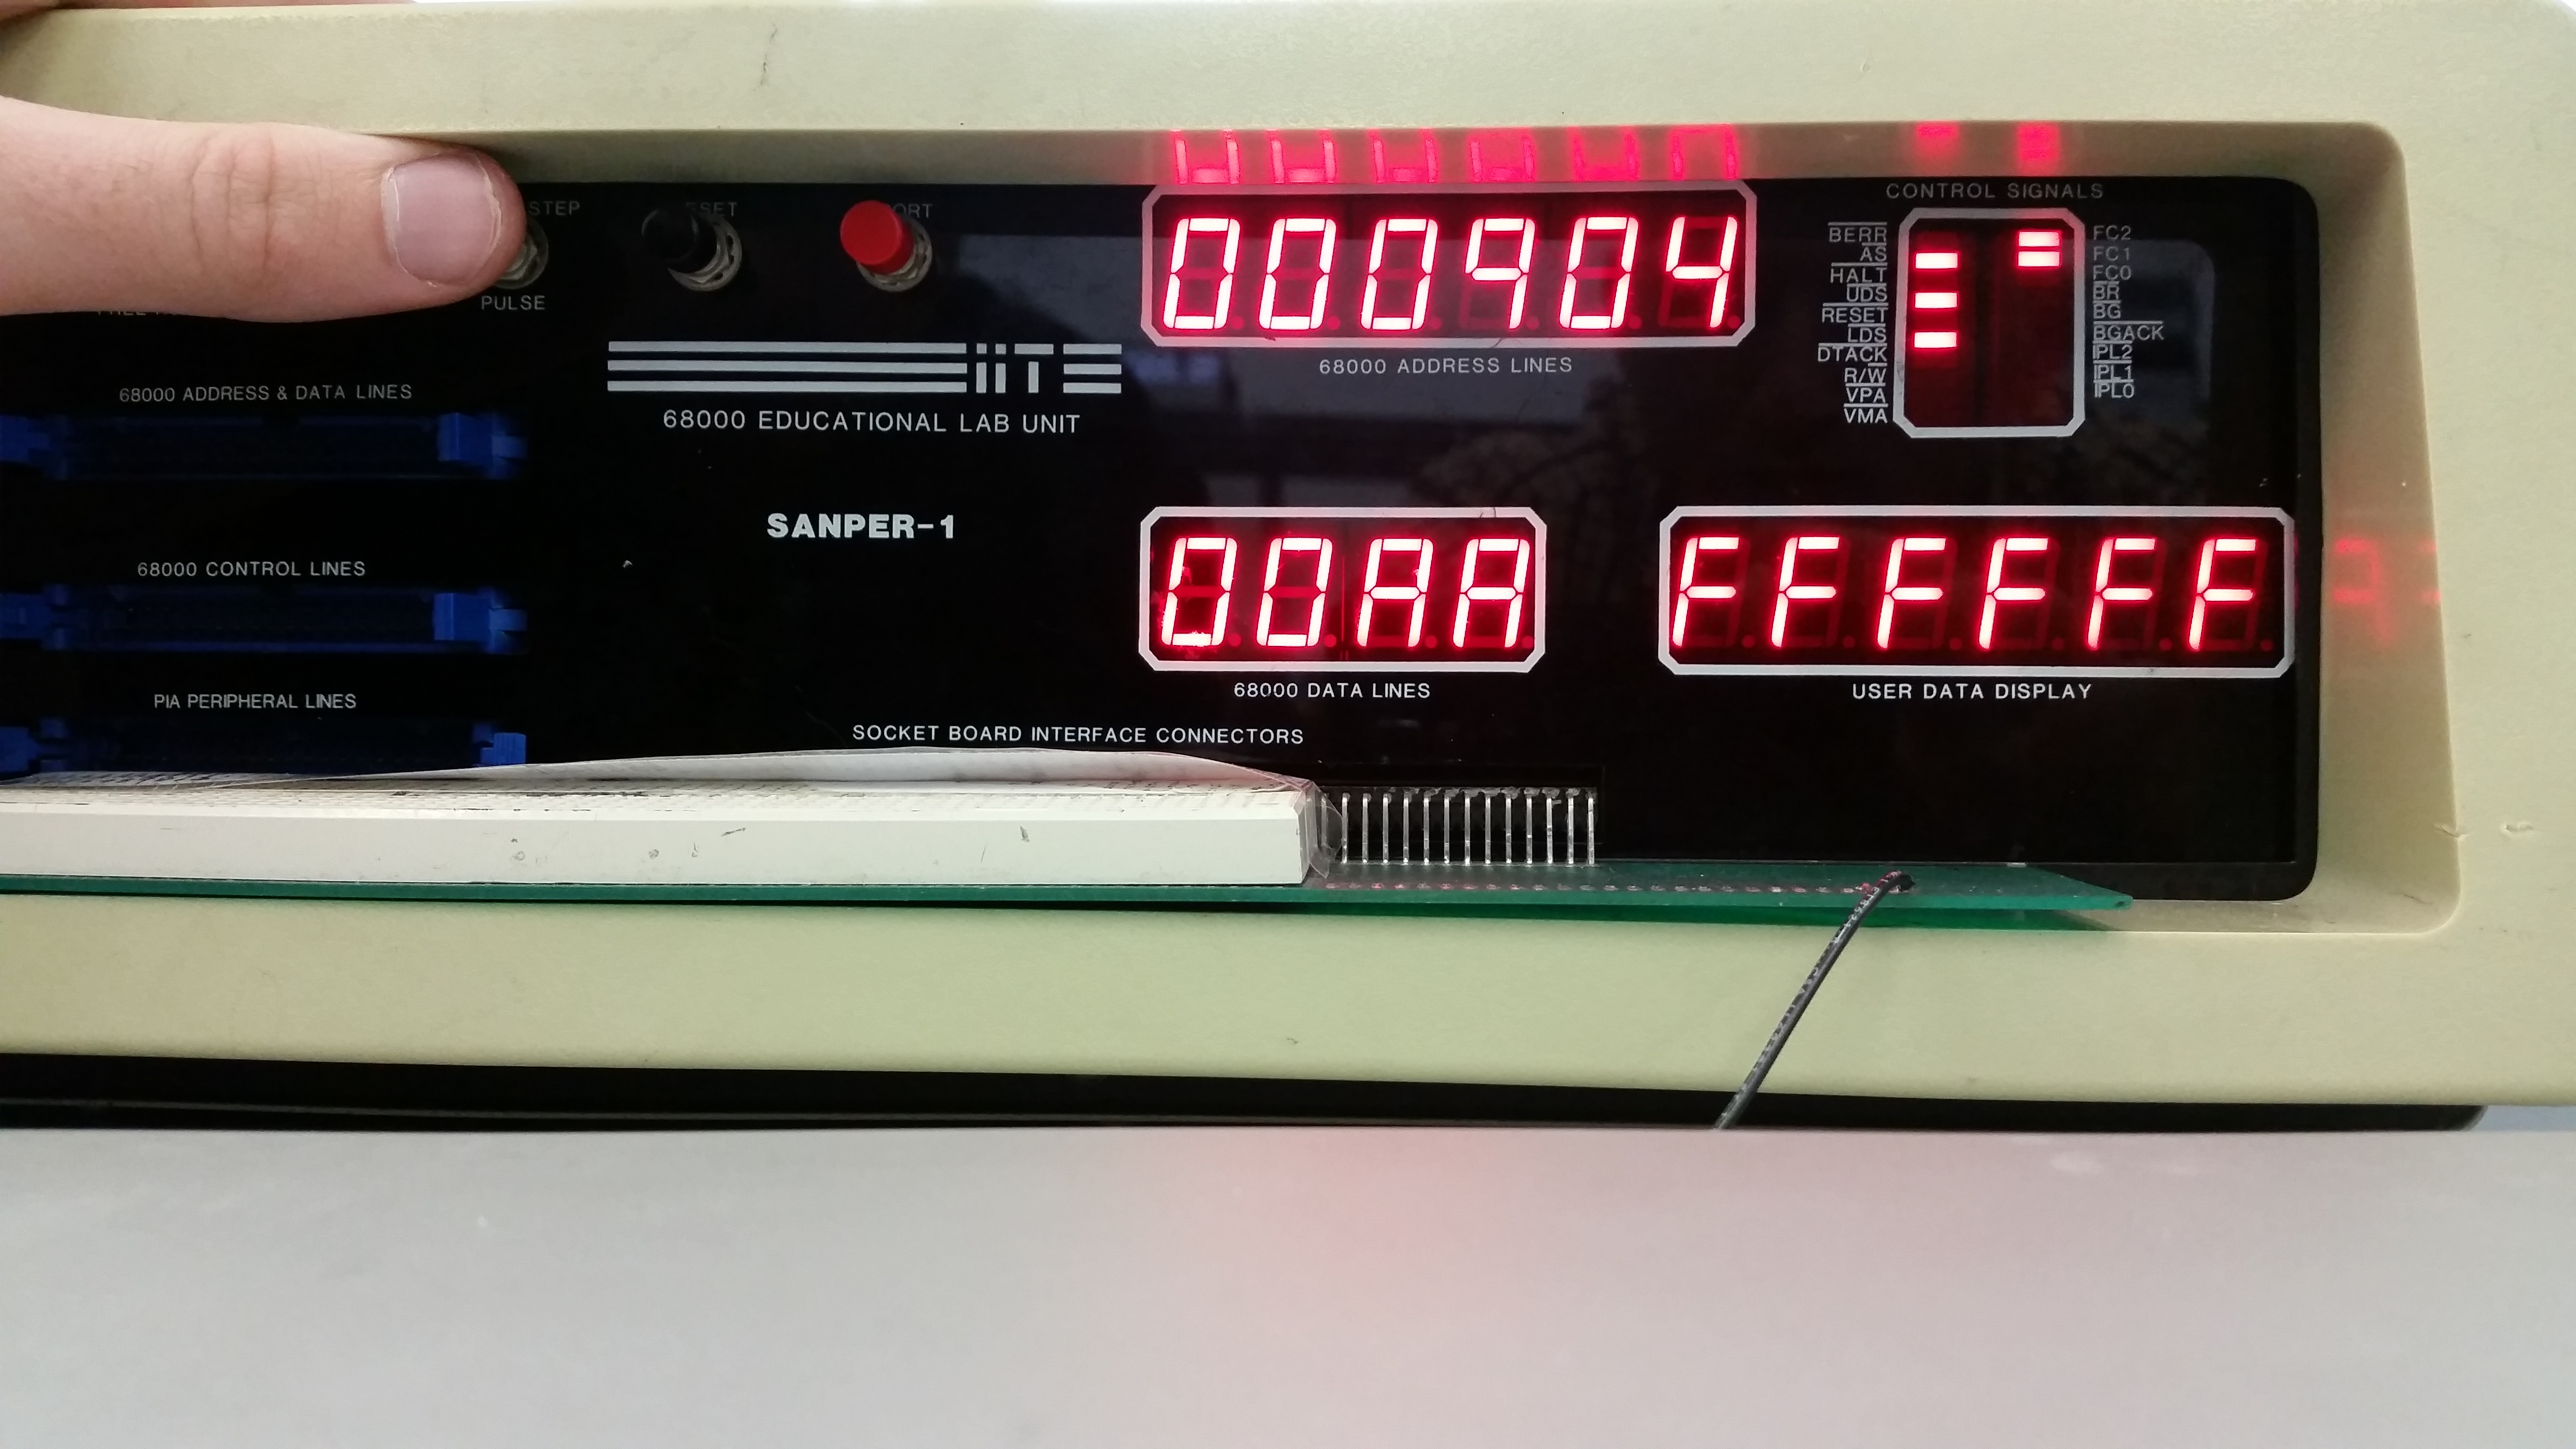
\includegraphics[width=1\linewidth]{Lab1/20150120_094642}
\end{center}
\begin{center}
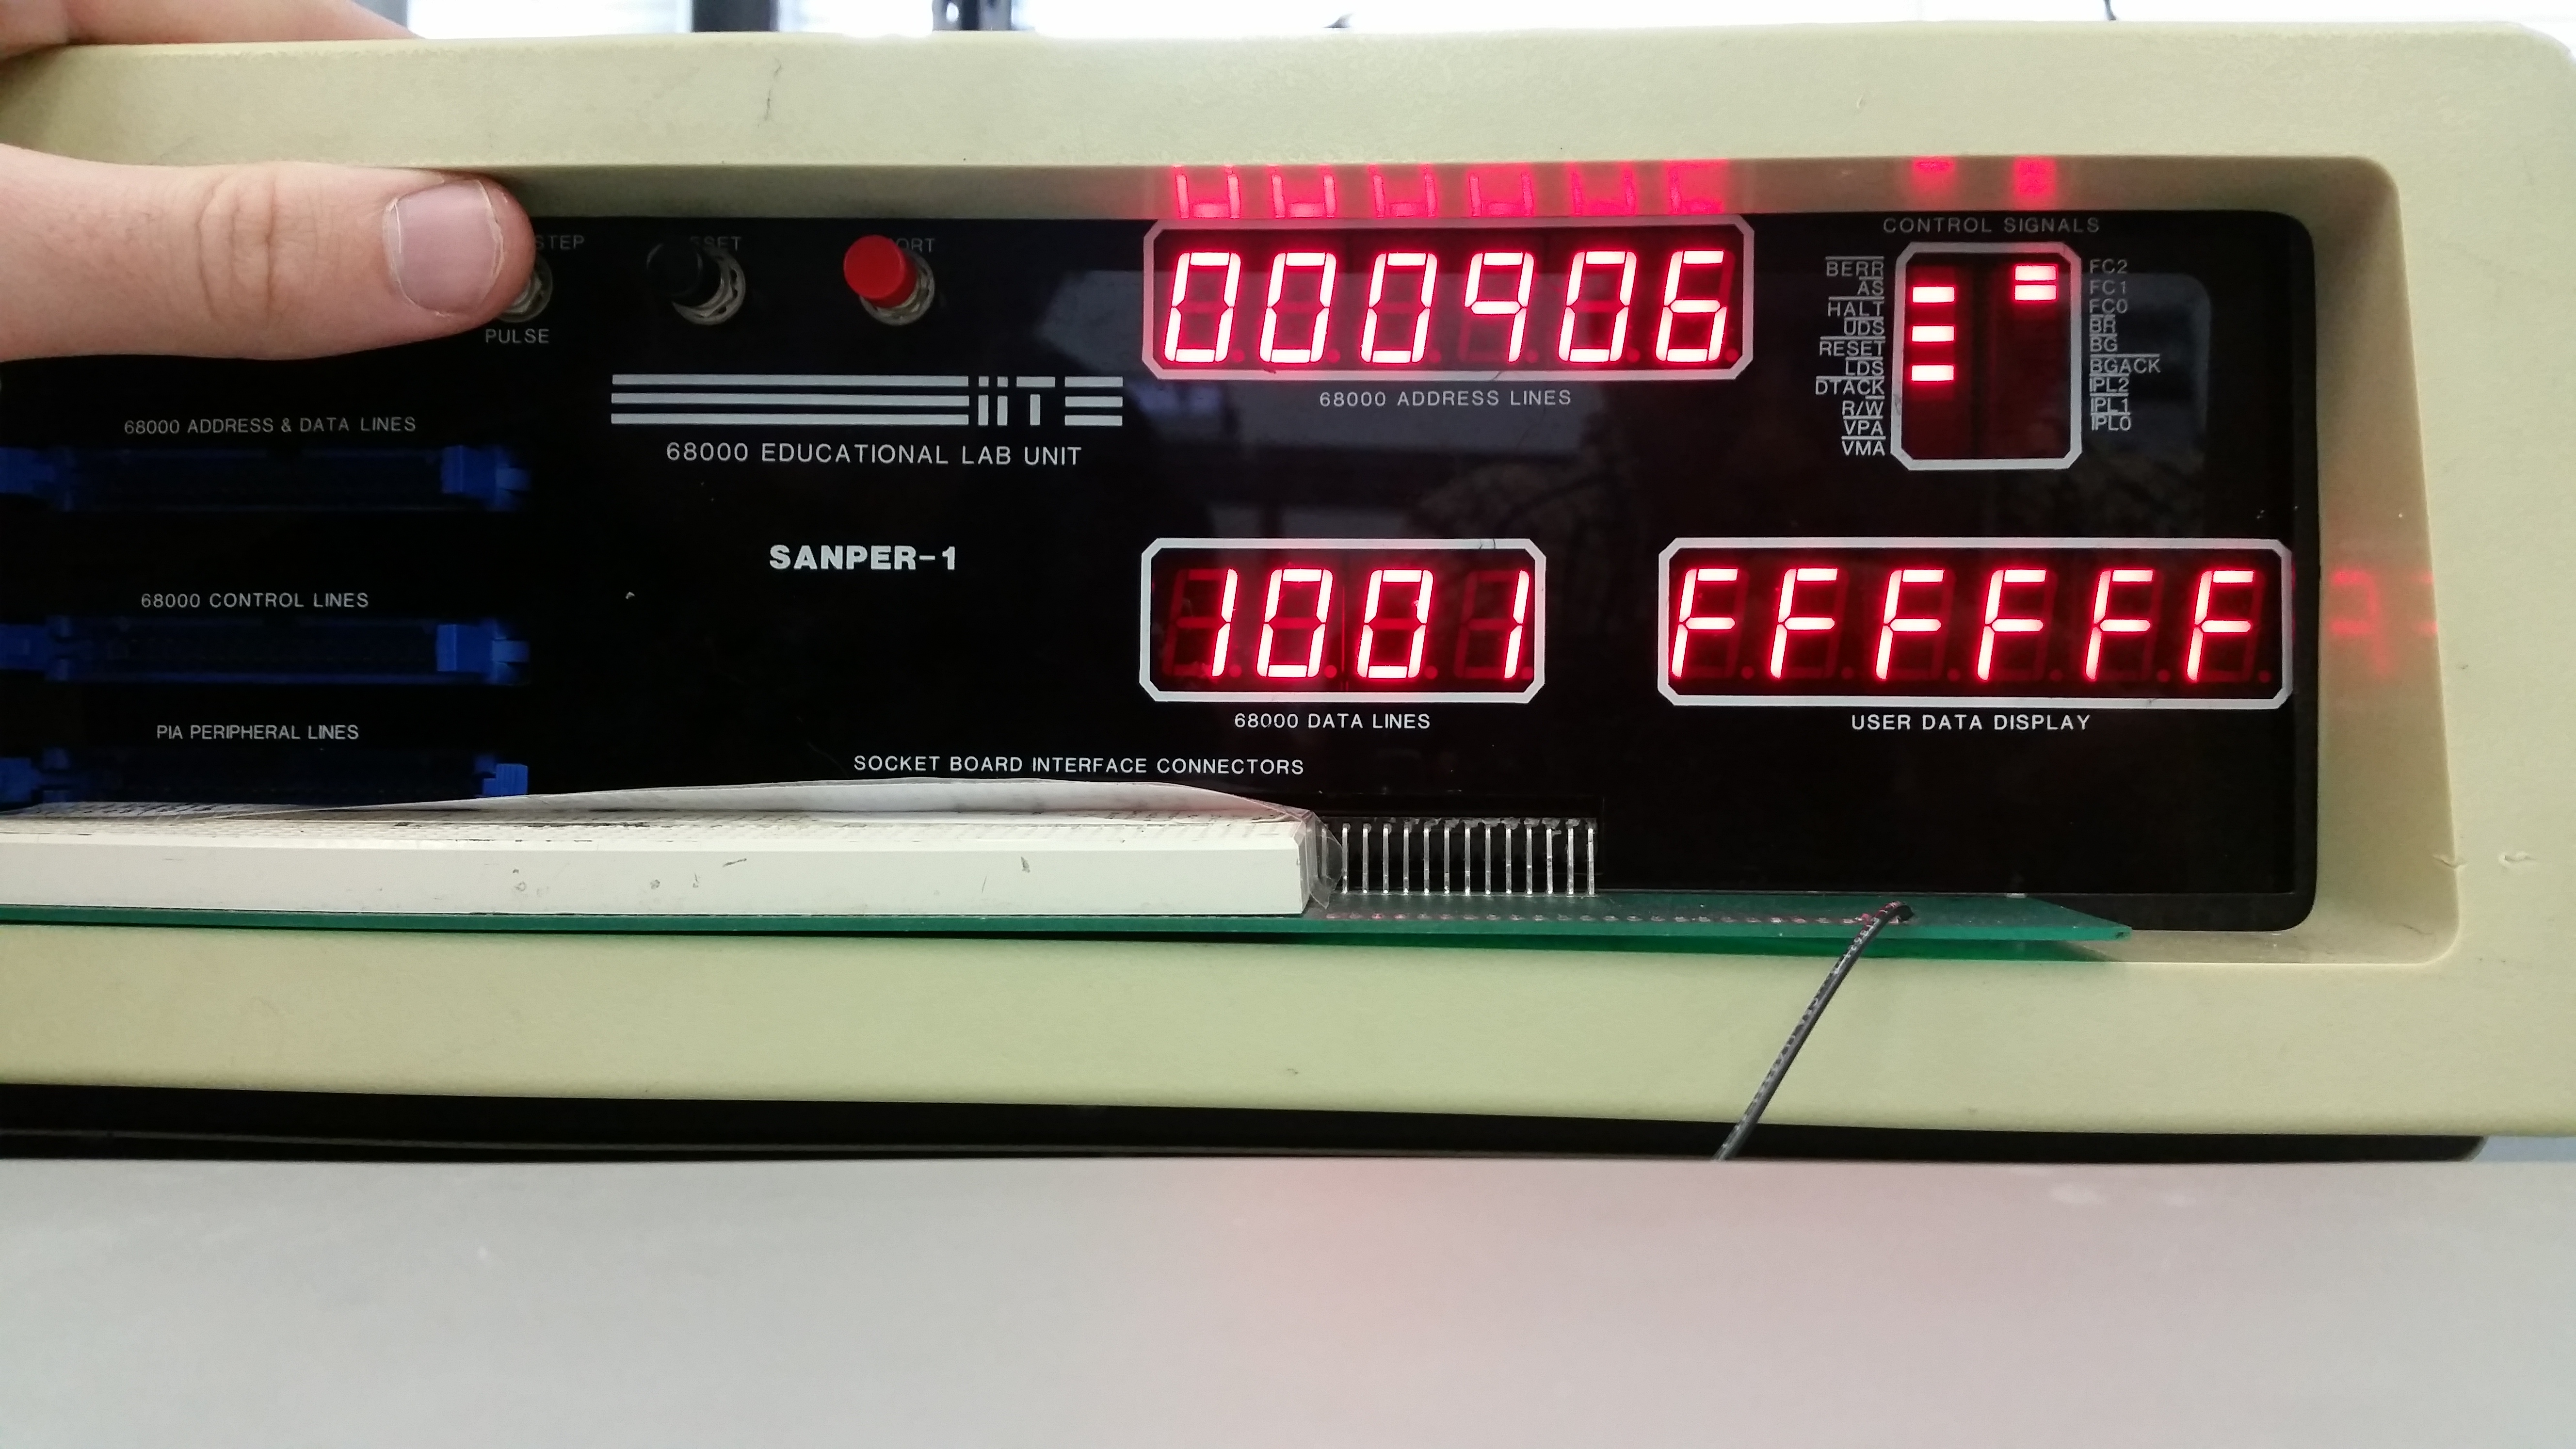
\includegraphics[width=1\linewidth]{Lab1/20150120_094644}
\end{center}
\begin{center}
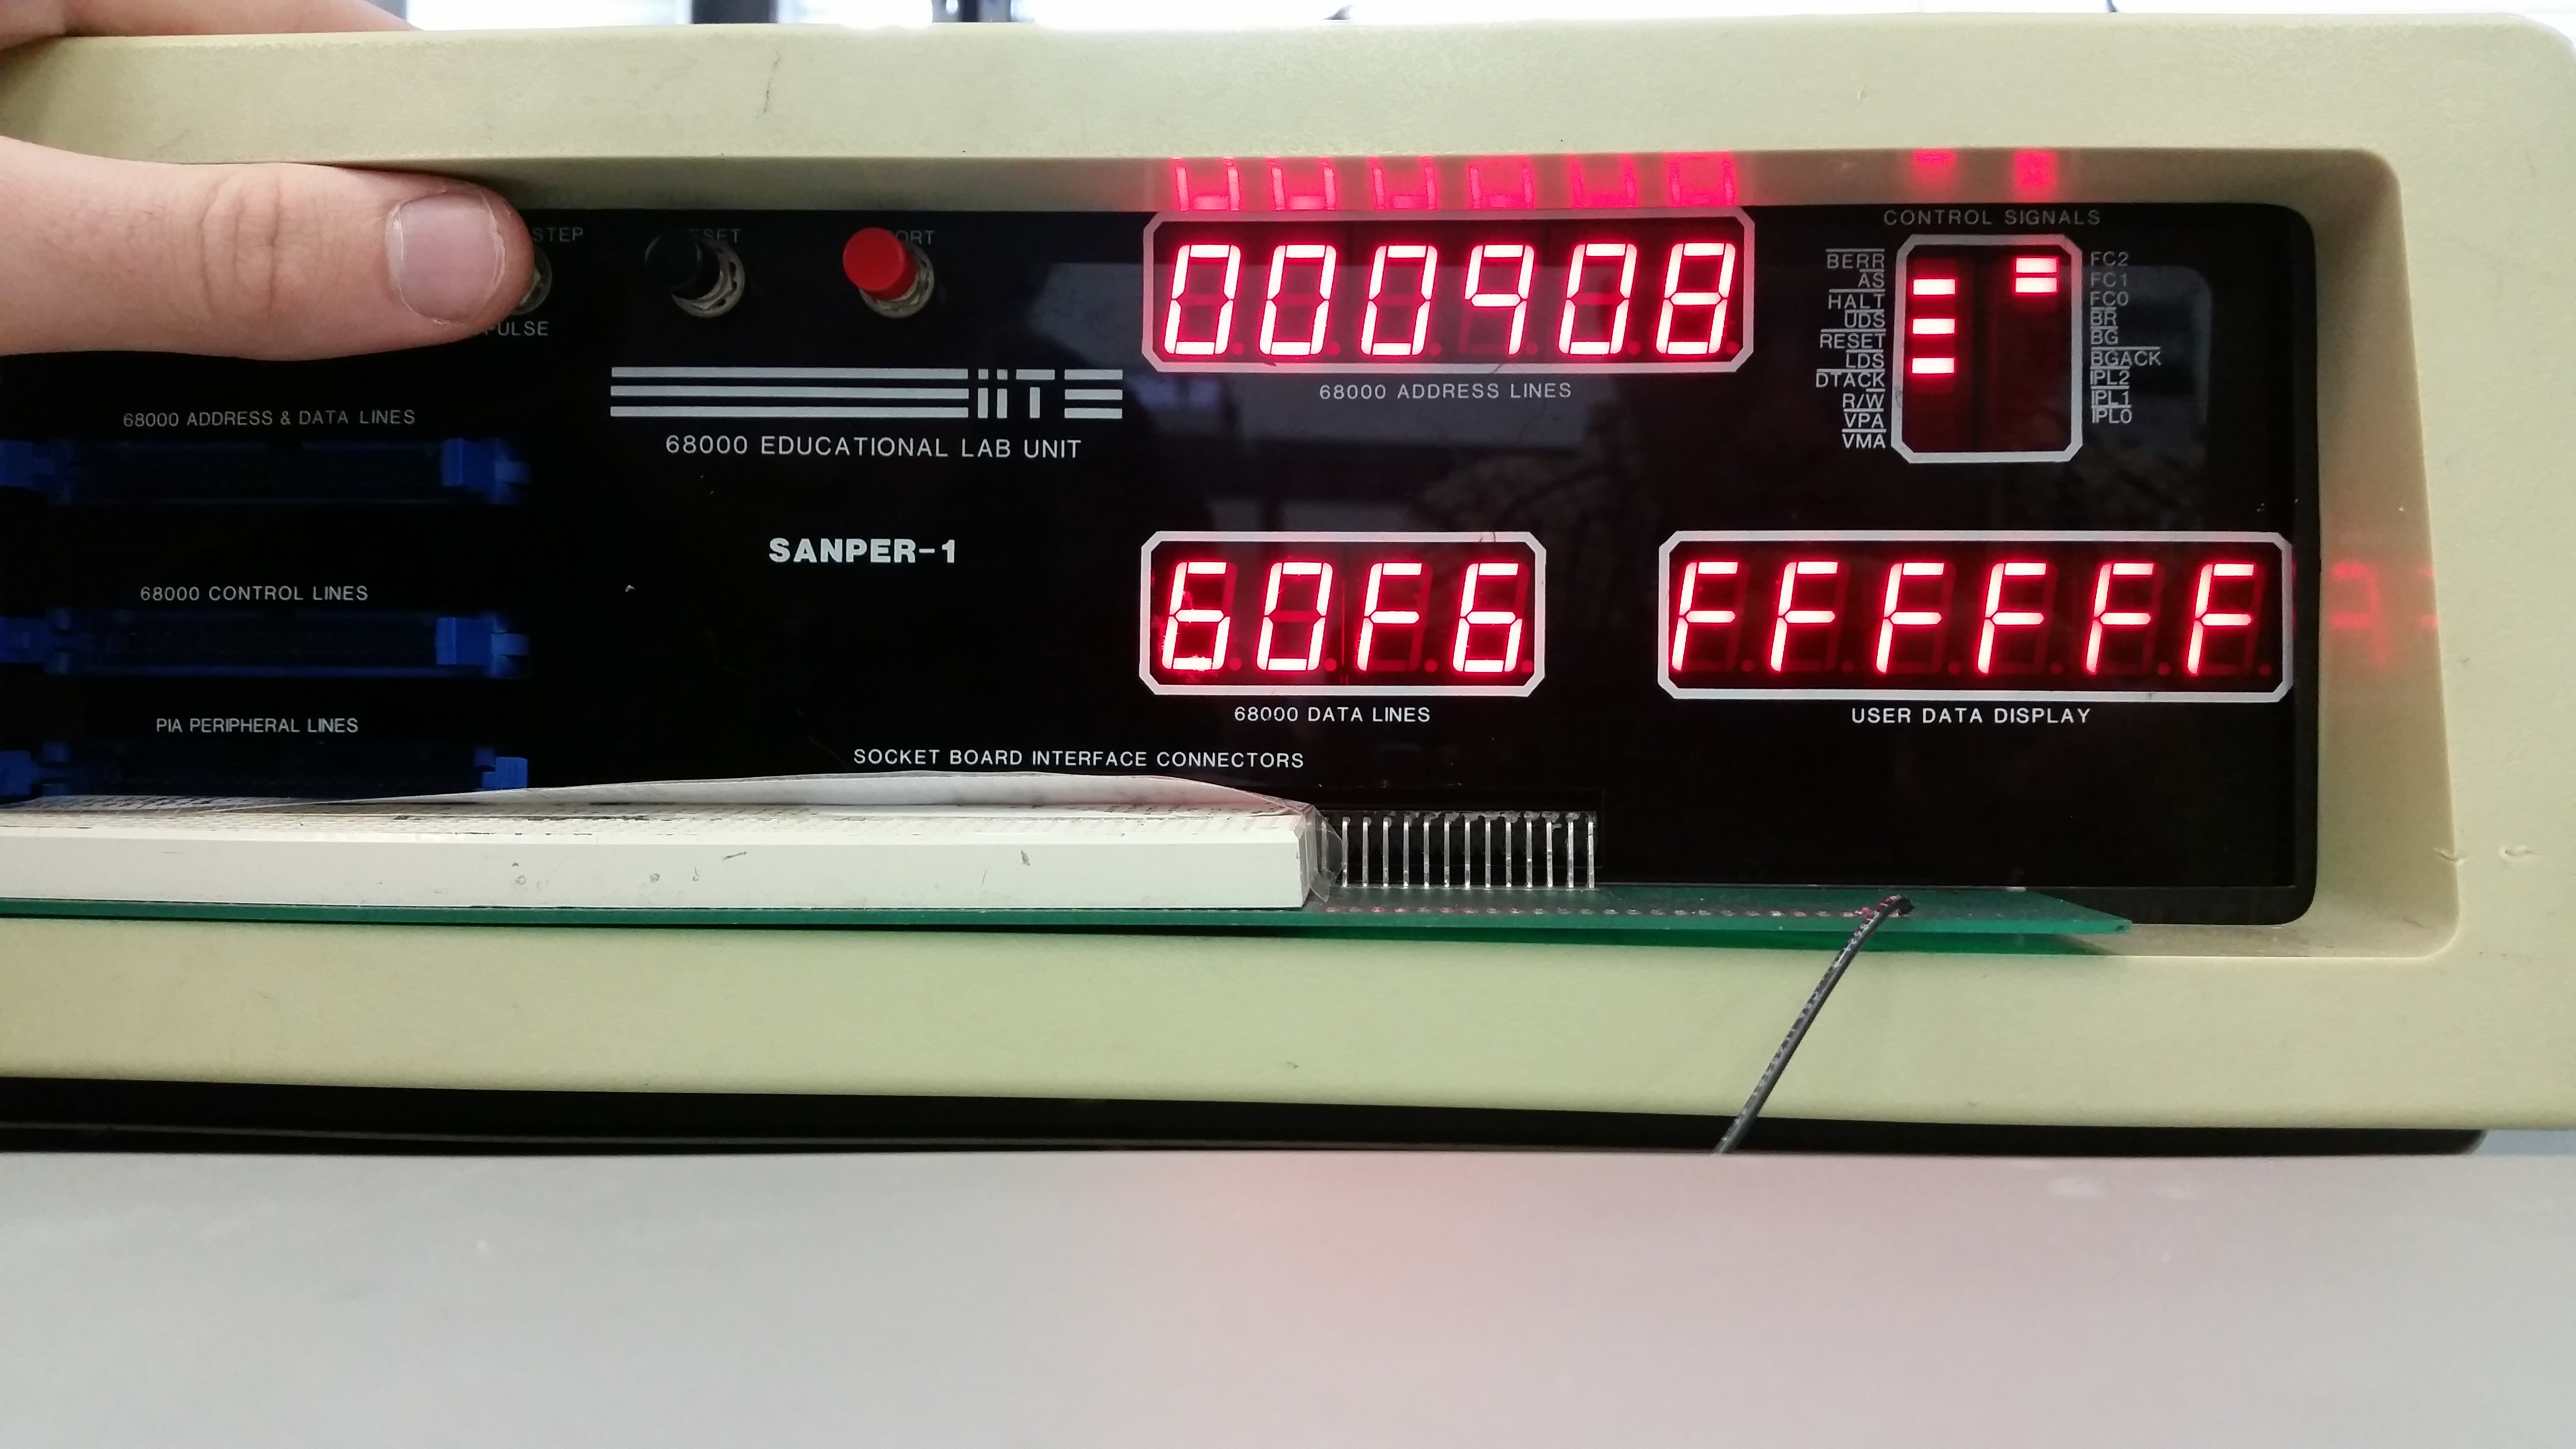
\includegraphics[width=1\linewidth]{Lab1/20150120_094646}
\end{center}
\begin{center}
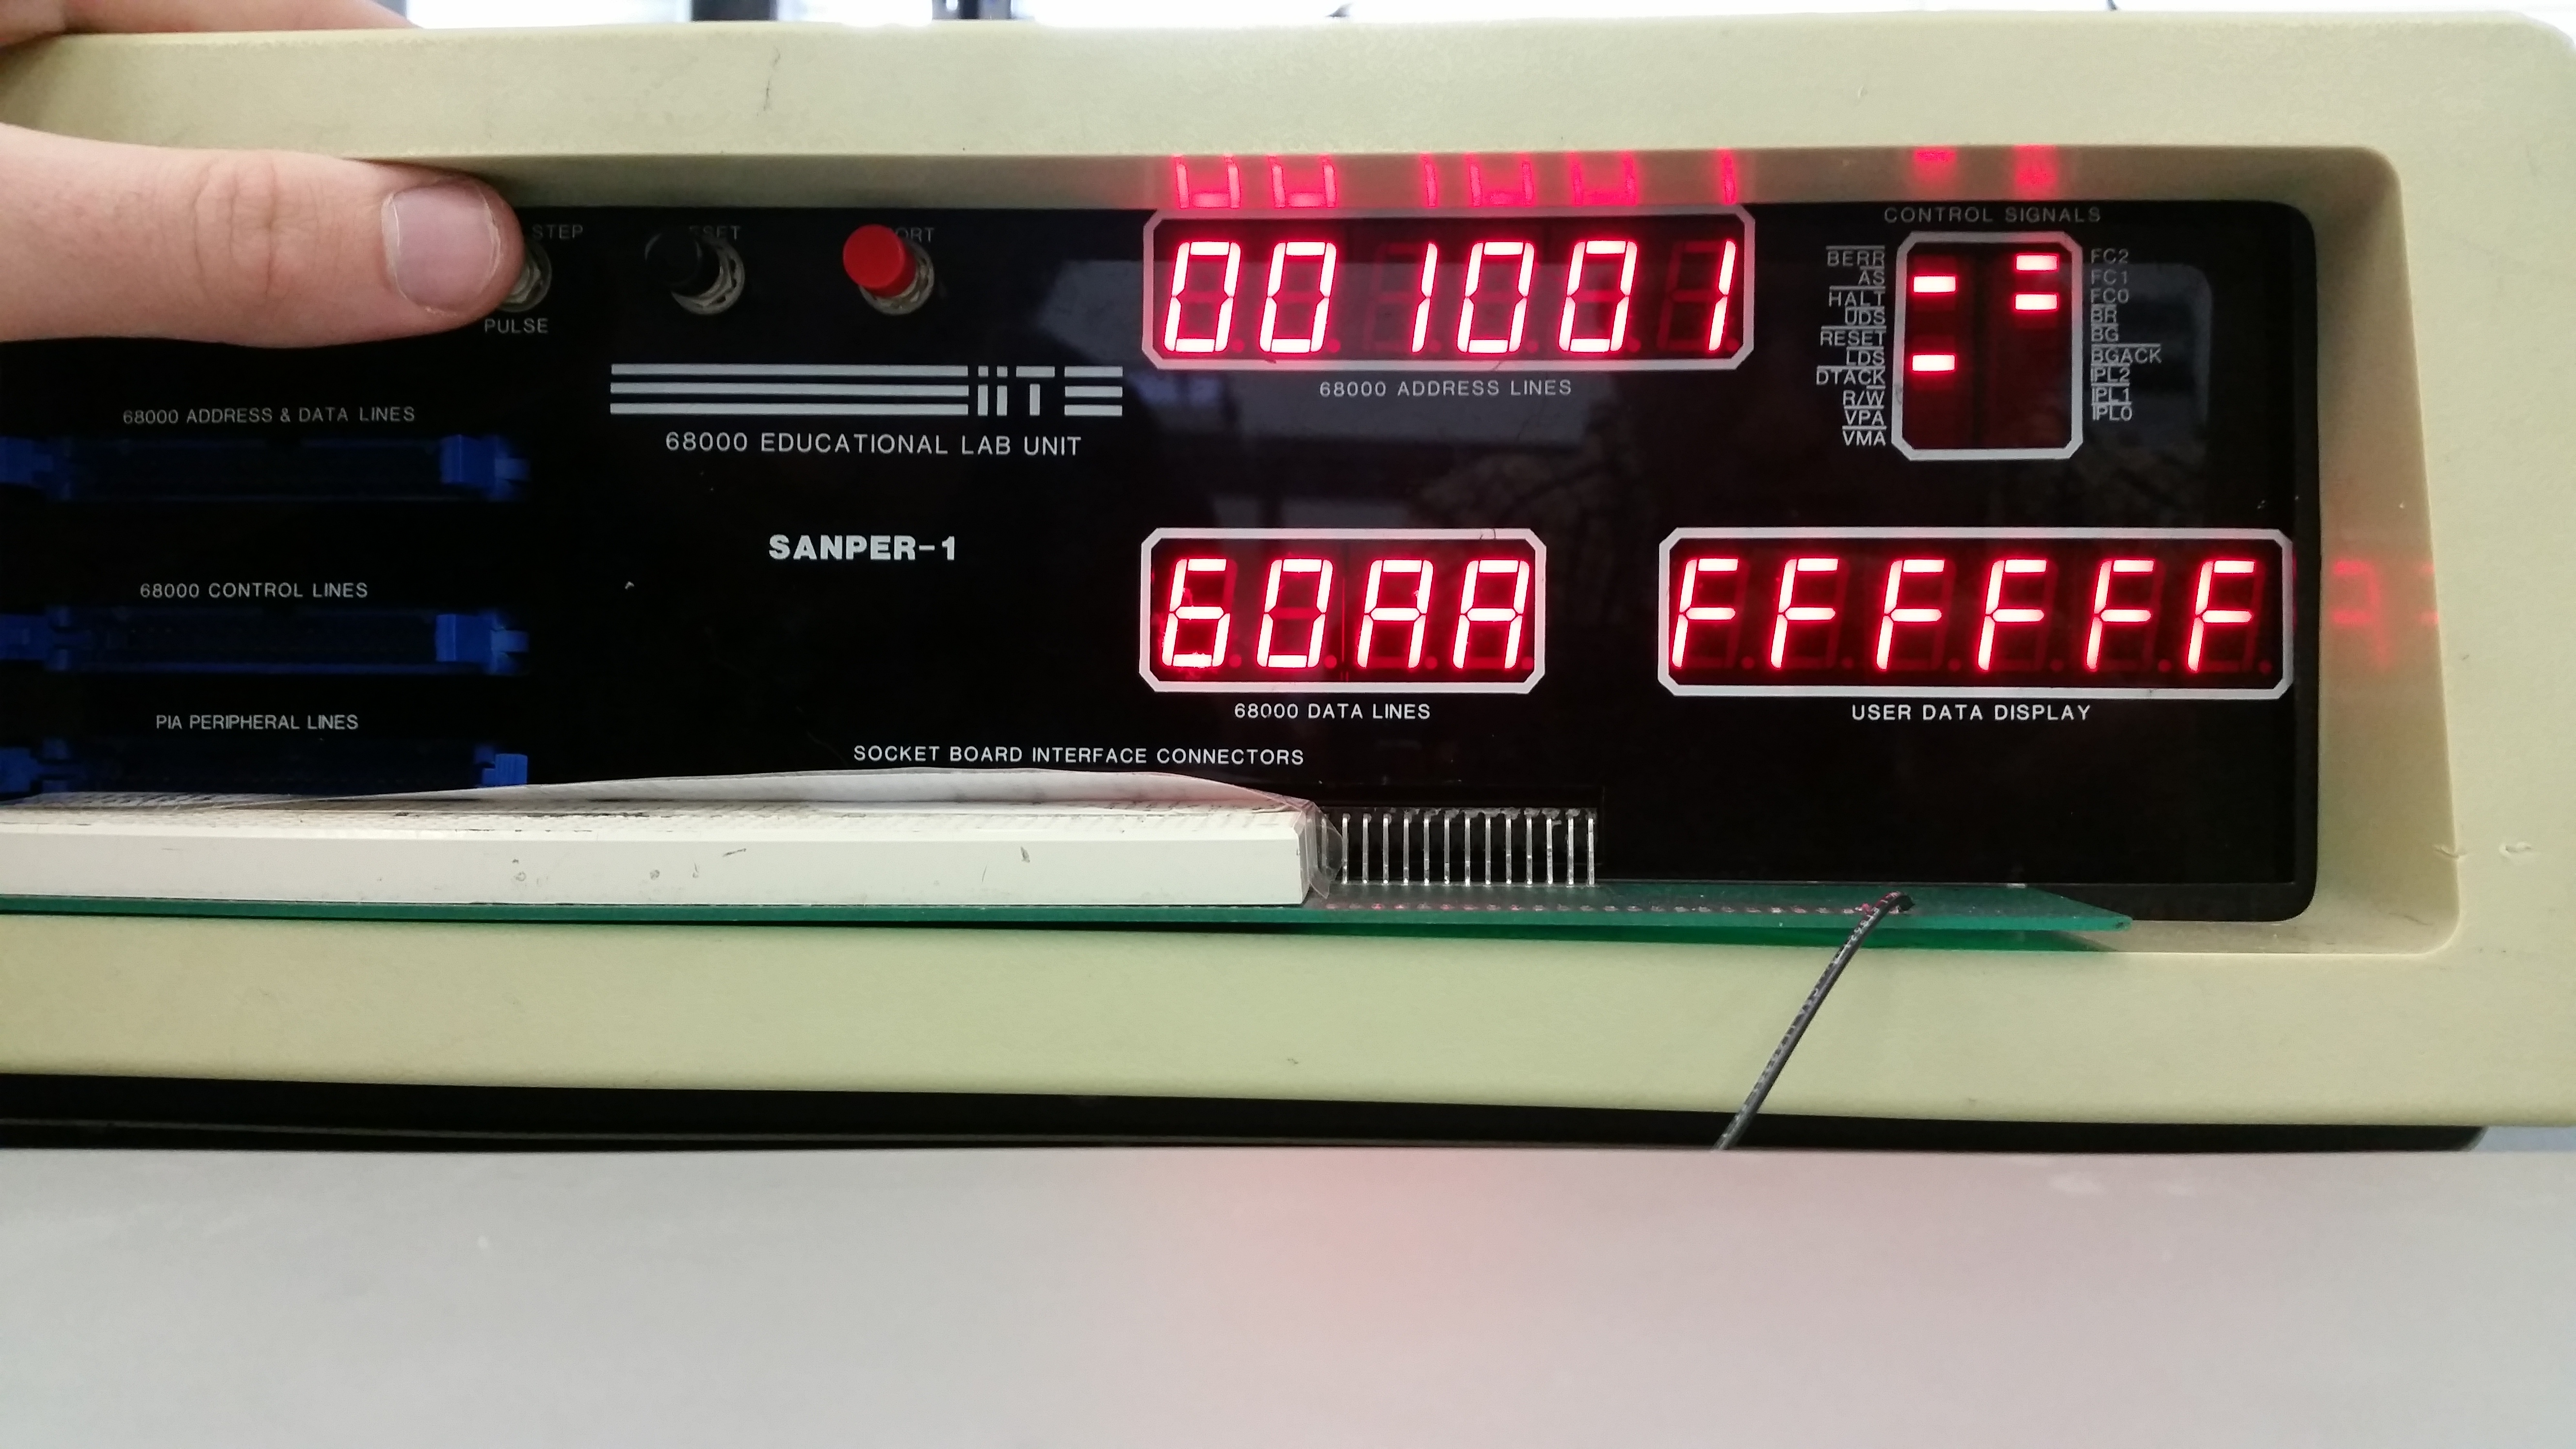
\includegraphics[width=1\linewidth]{Lab1/20150120_094648}
\end{center}
\begin{center}
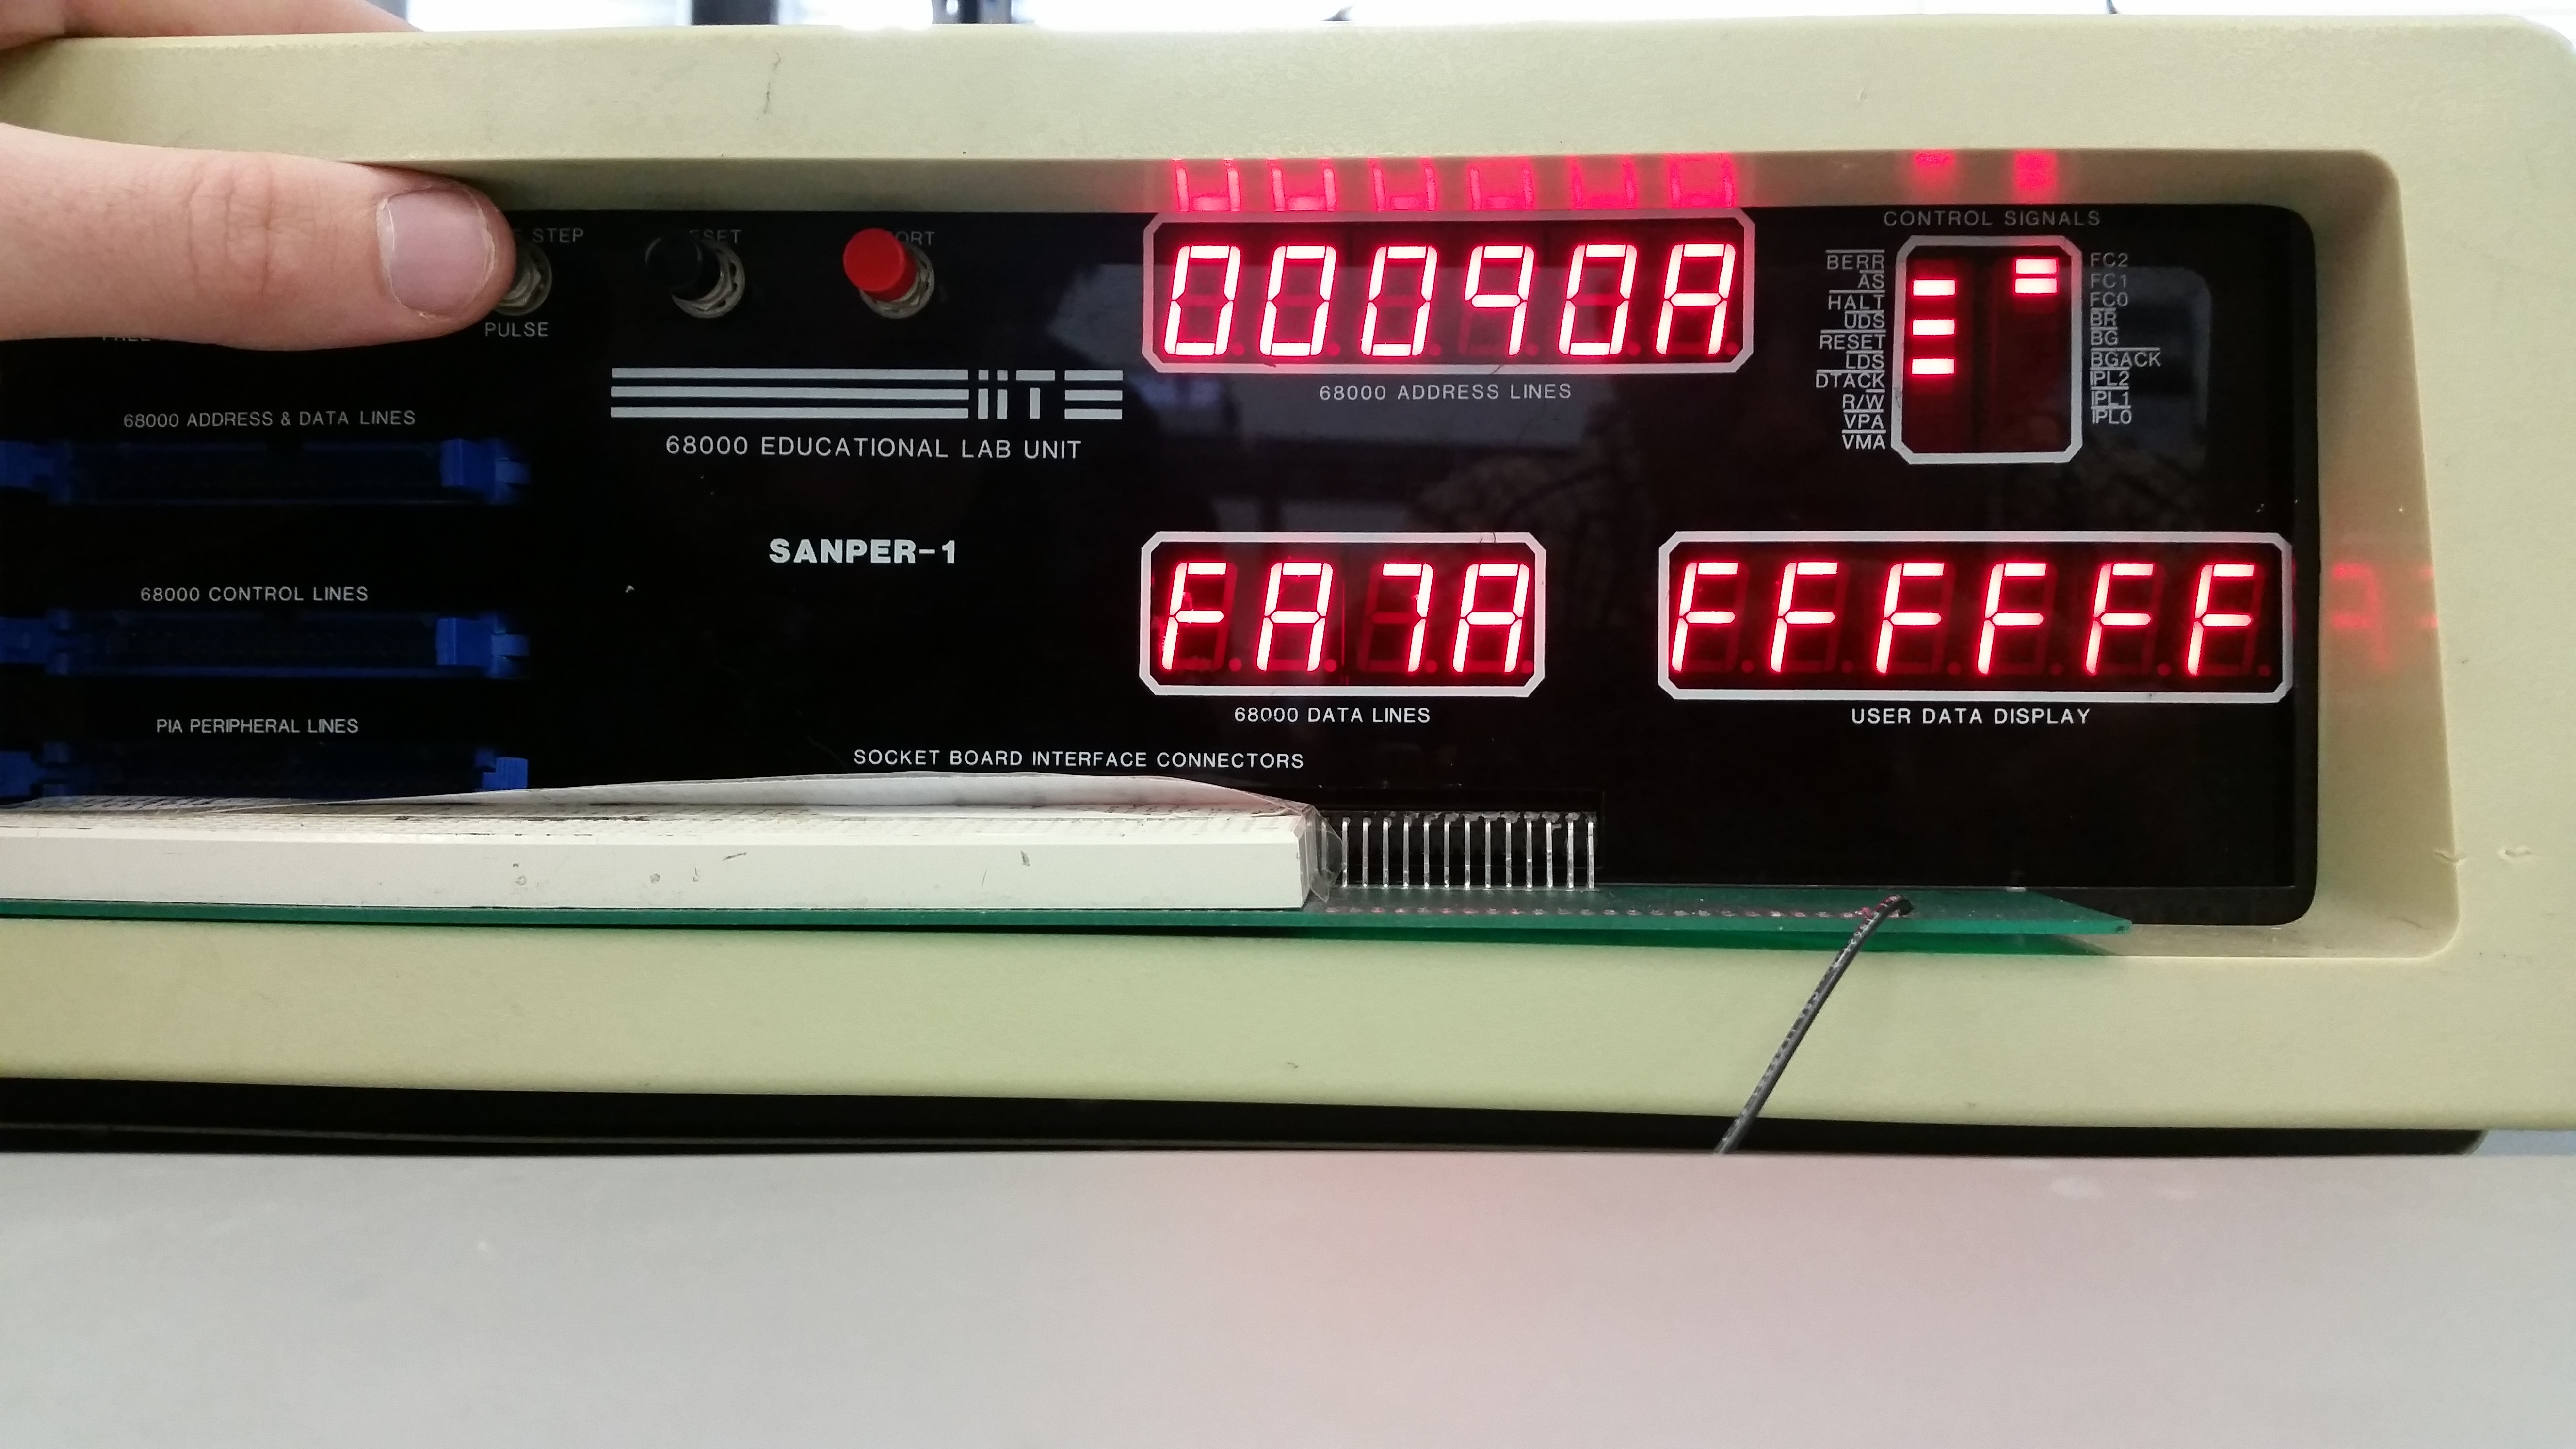
\includegraphics[width=1\linewidth]{Lab1/20150120_094649}
\end{center}
\begin{center}
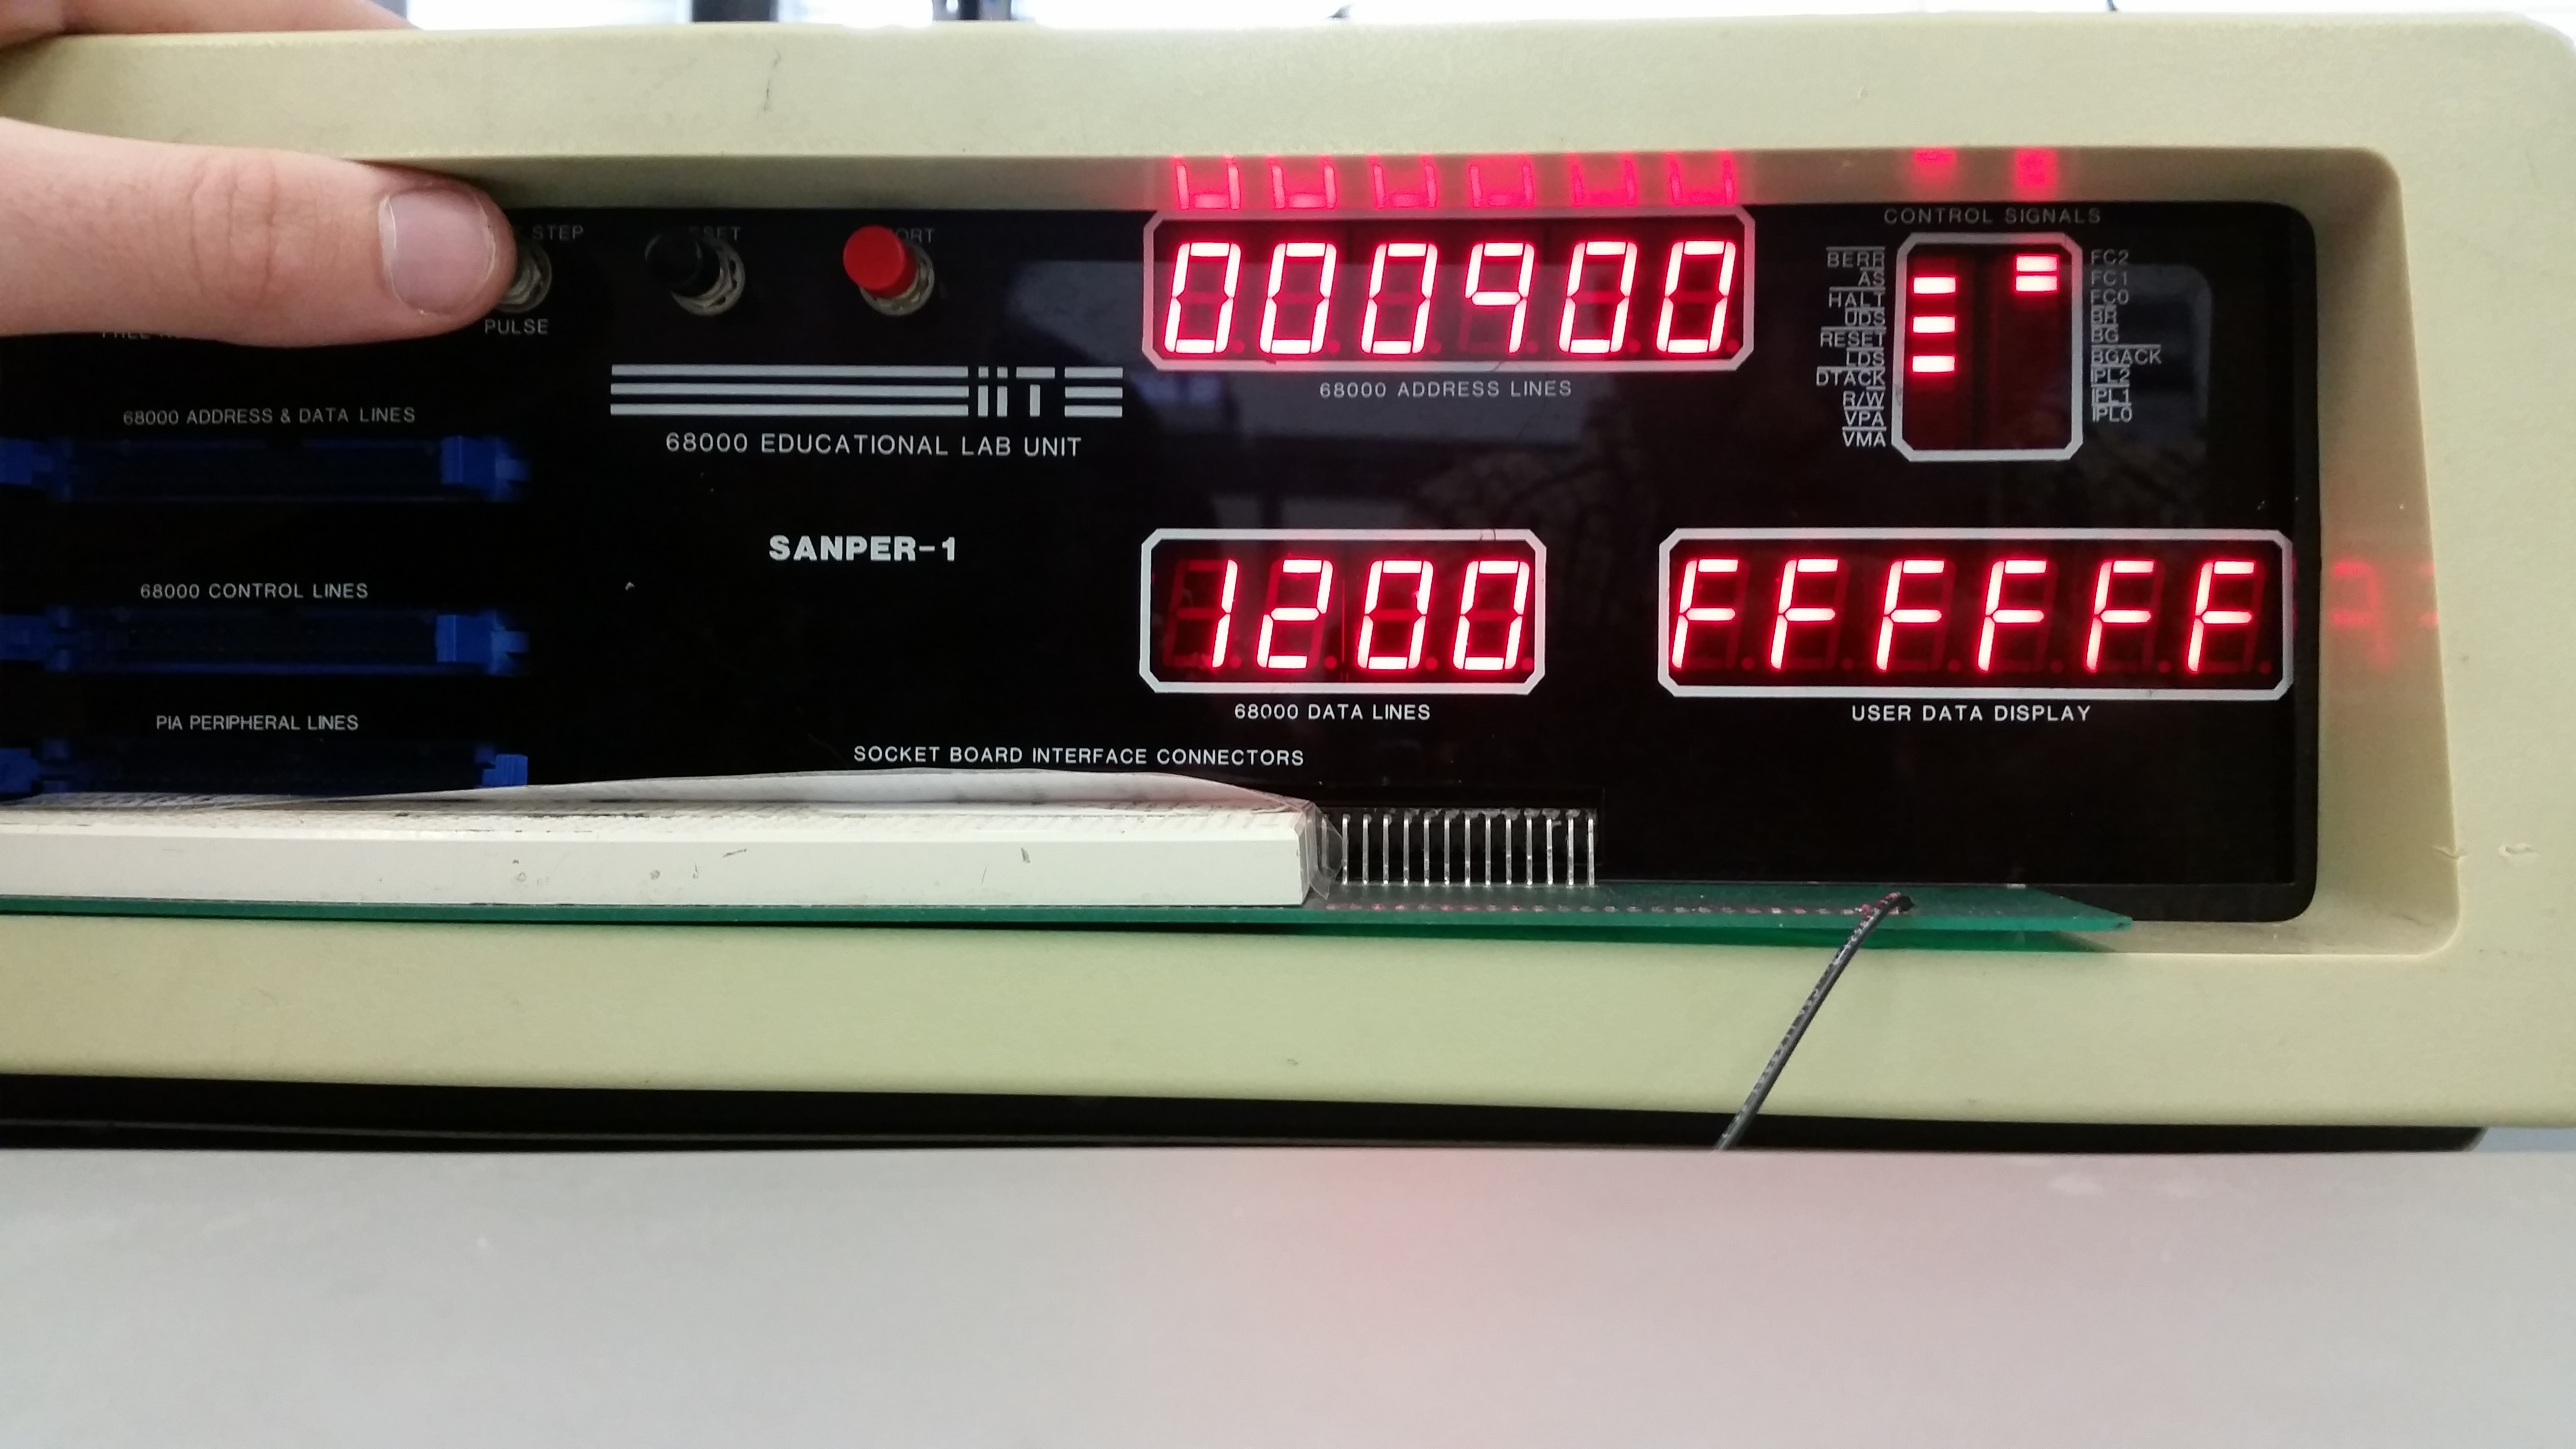
\includegraphics[width=1\linewidth]{Lab1/20150120_094651}
\end{center}
\subsubsection{Program 4}
\label{progpic4}
\begin{center}
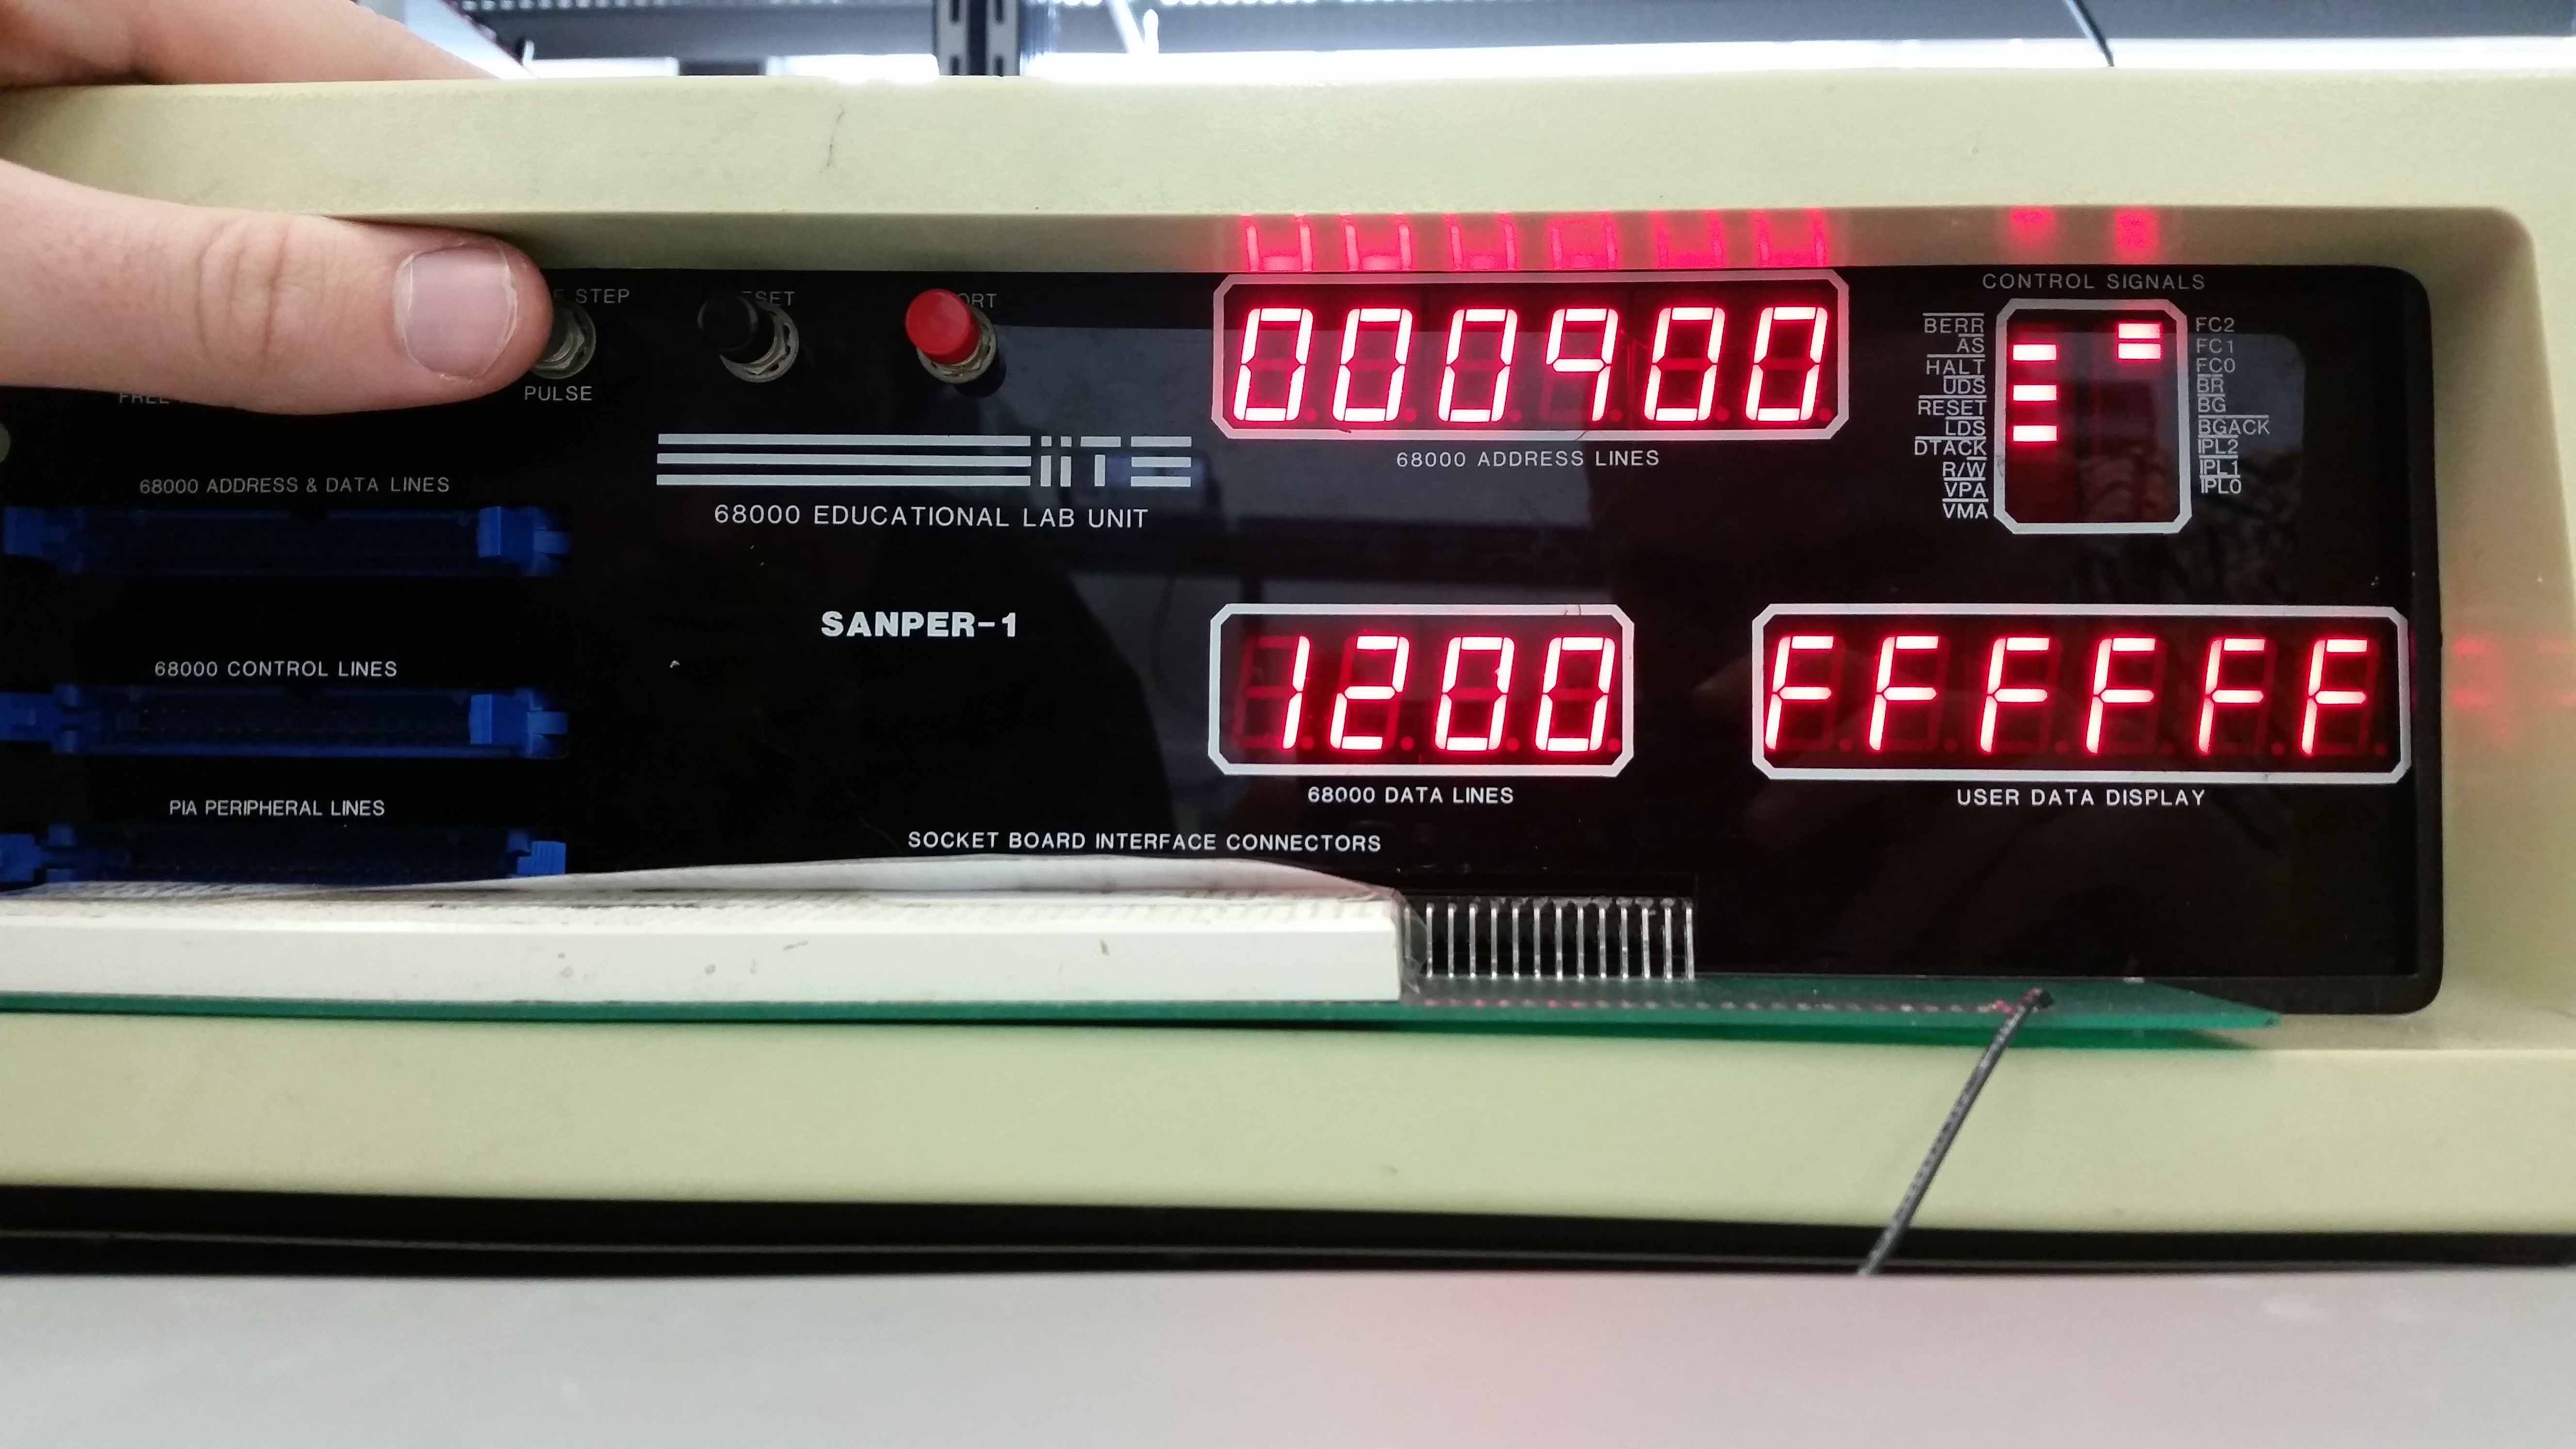
\includegraphics[width=1\linewidth]{Lab1/20150120_094835}
\end{center}
\begin{center}
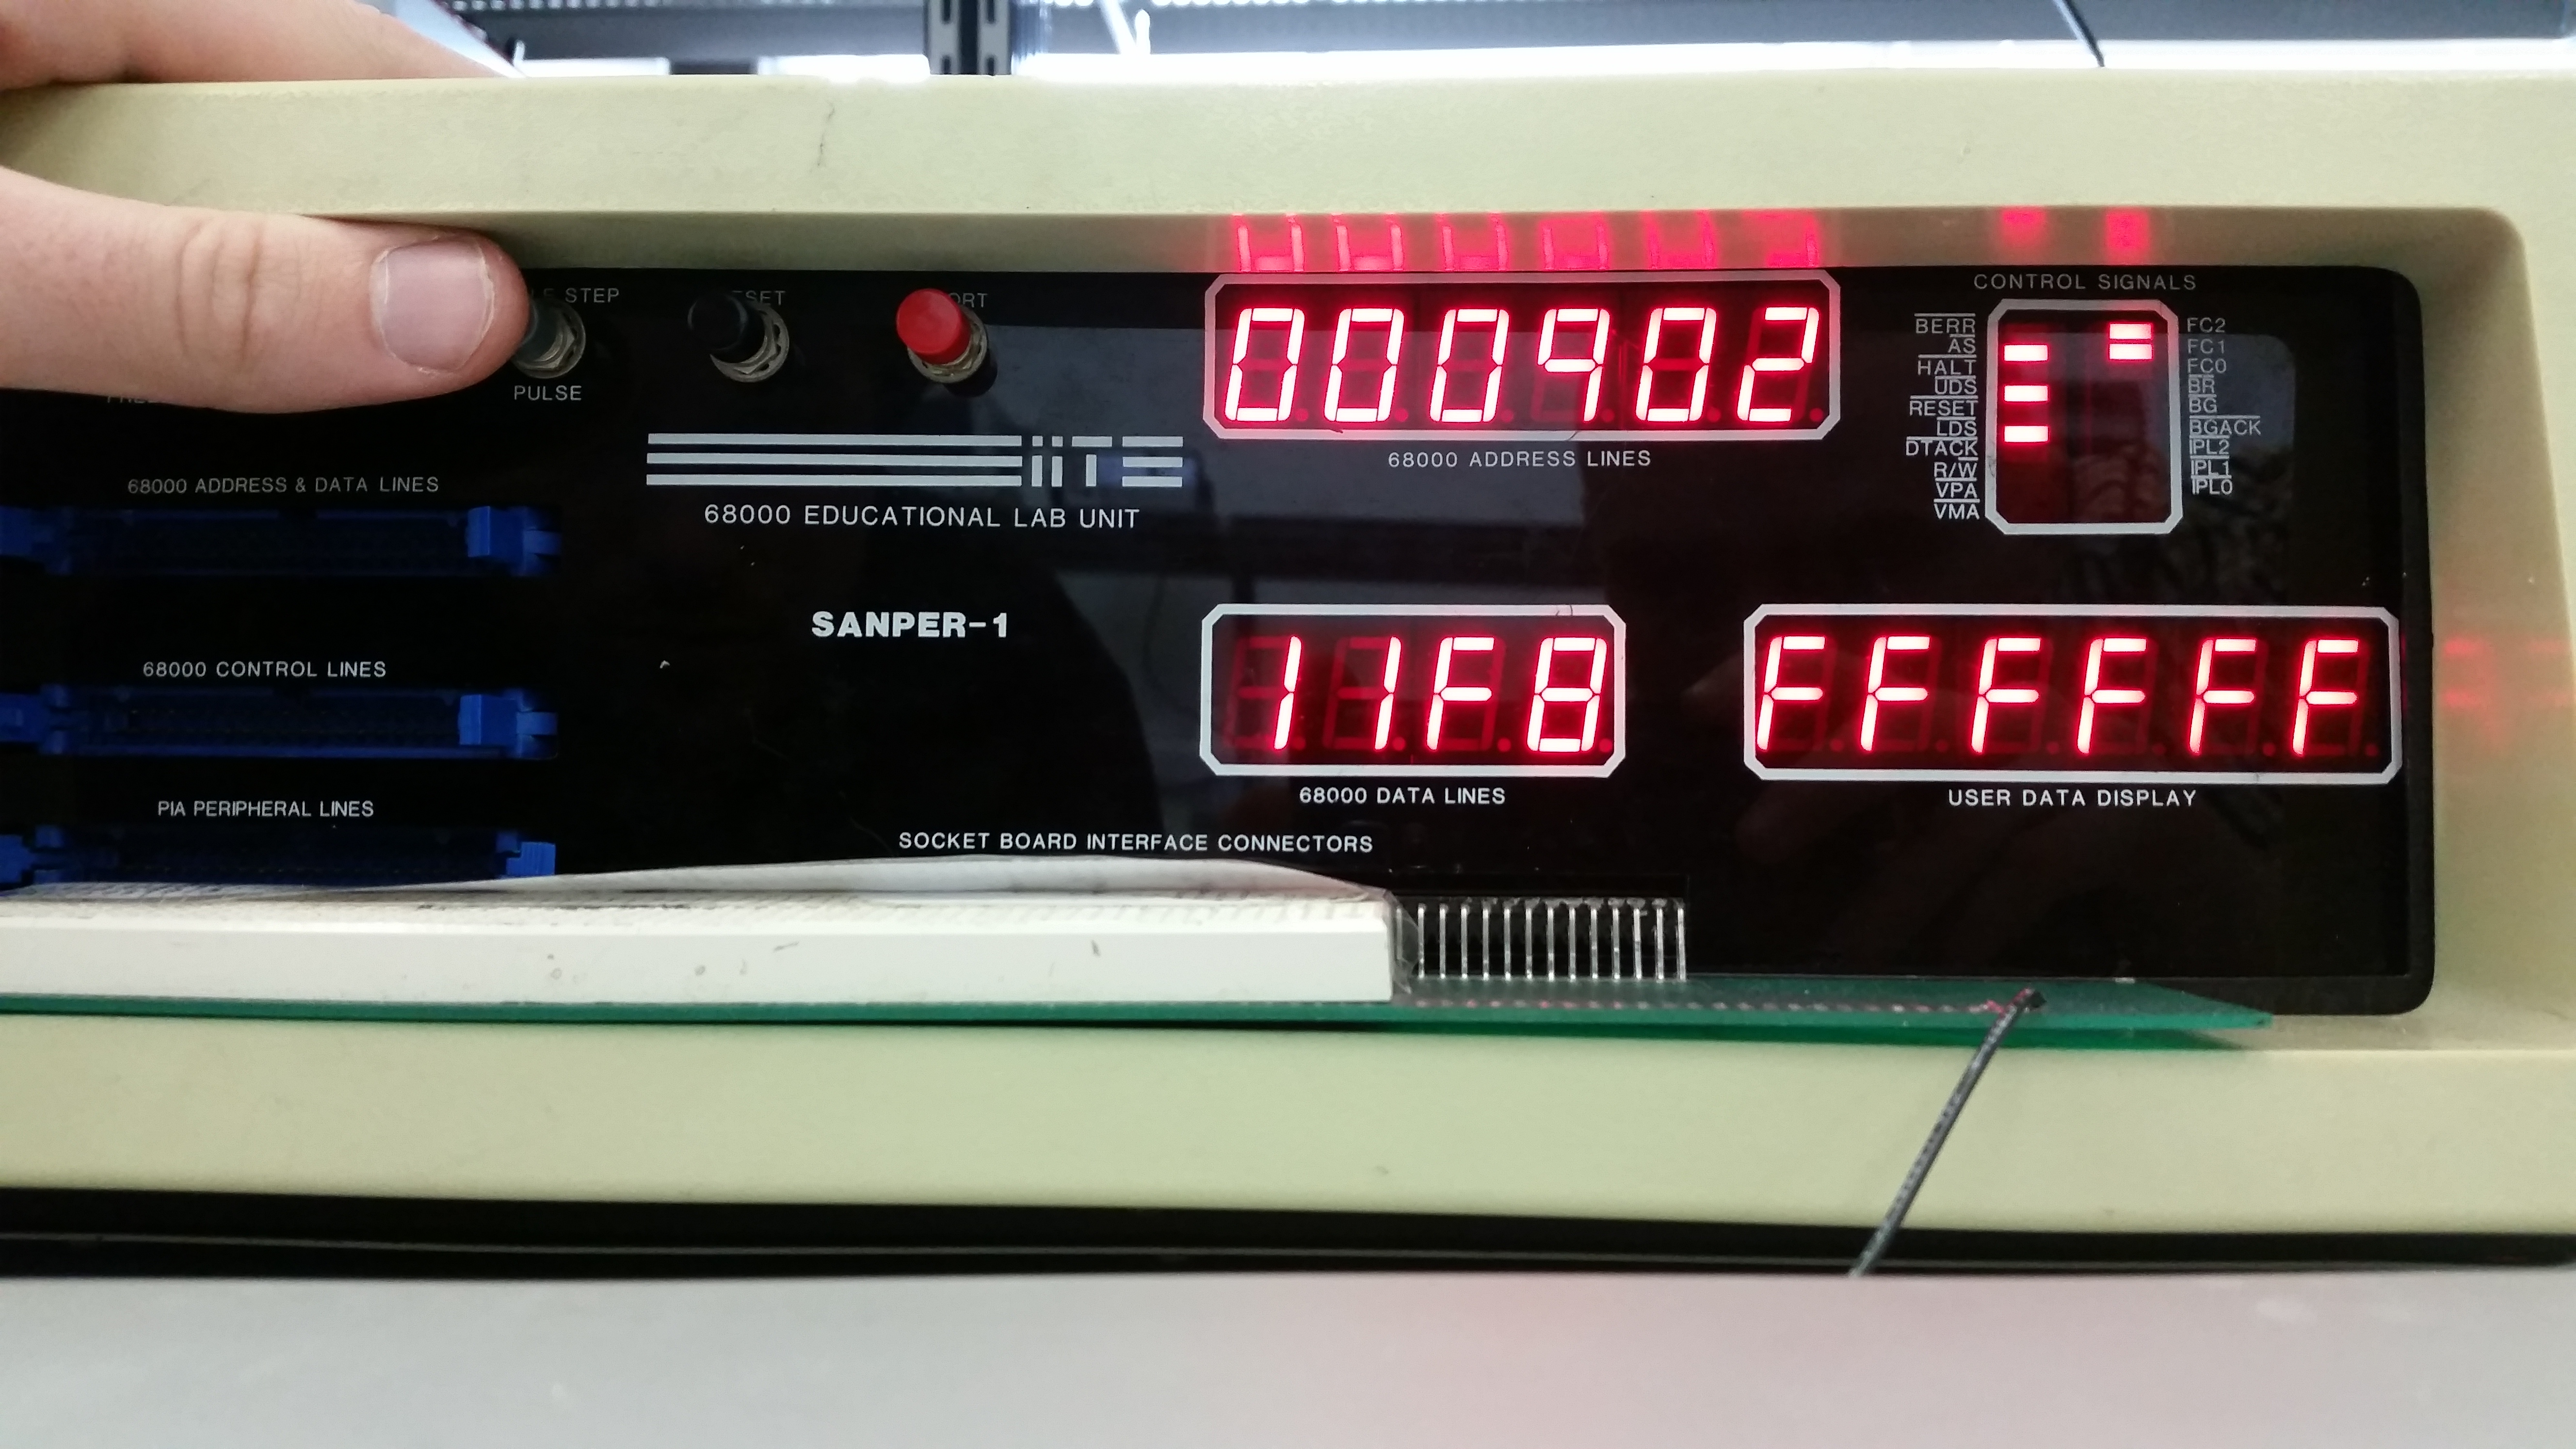
\includegraphics[width=1\linewidth]{Lab1/20150120_094837}
\end{center}
\begin{center}
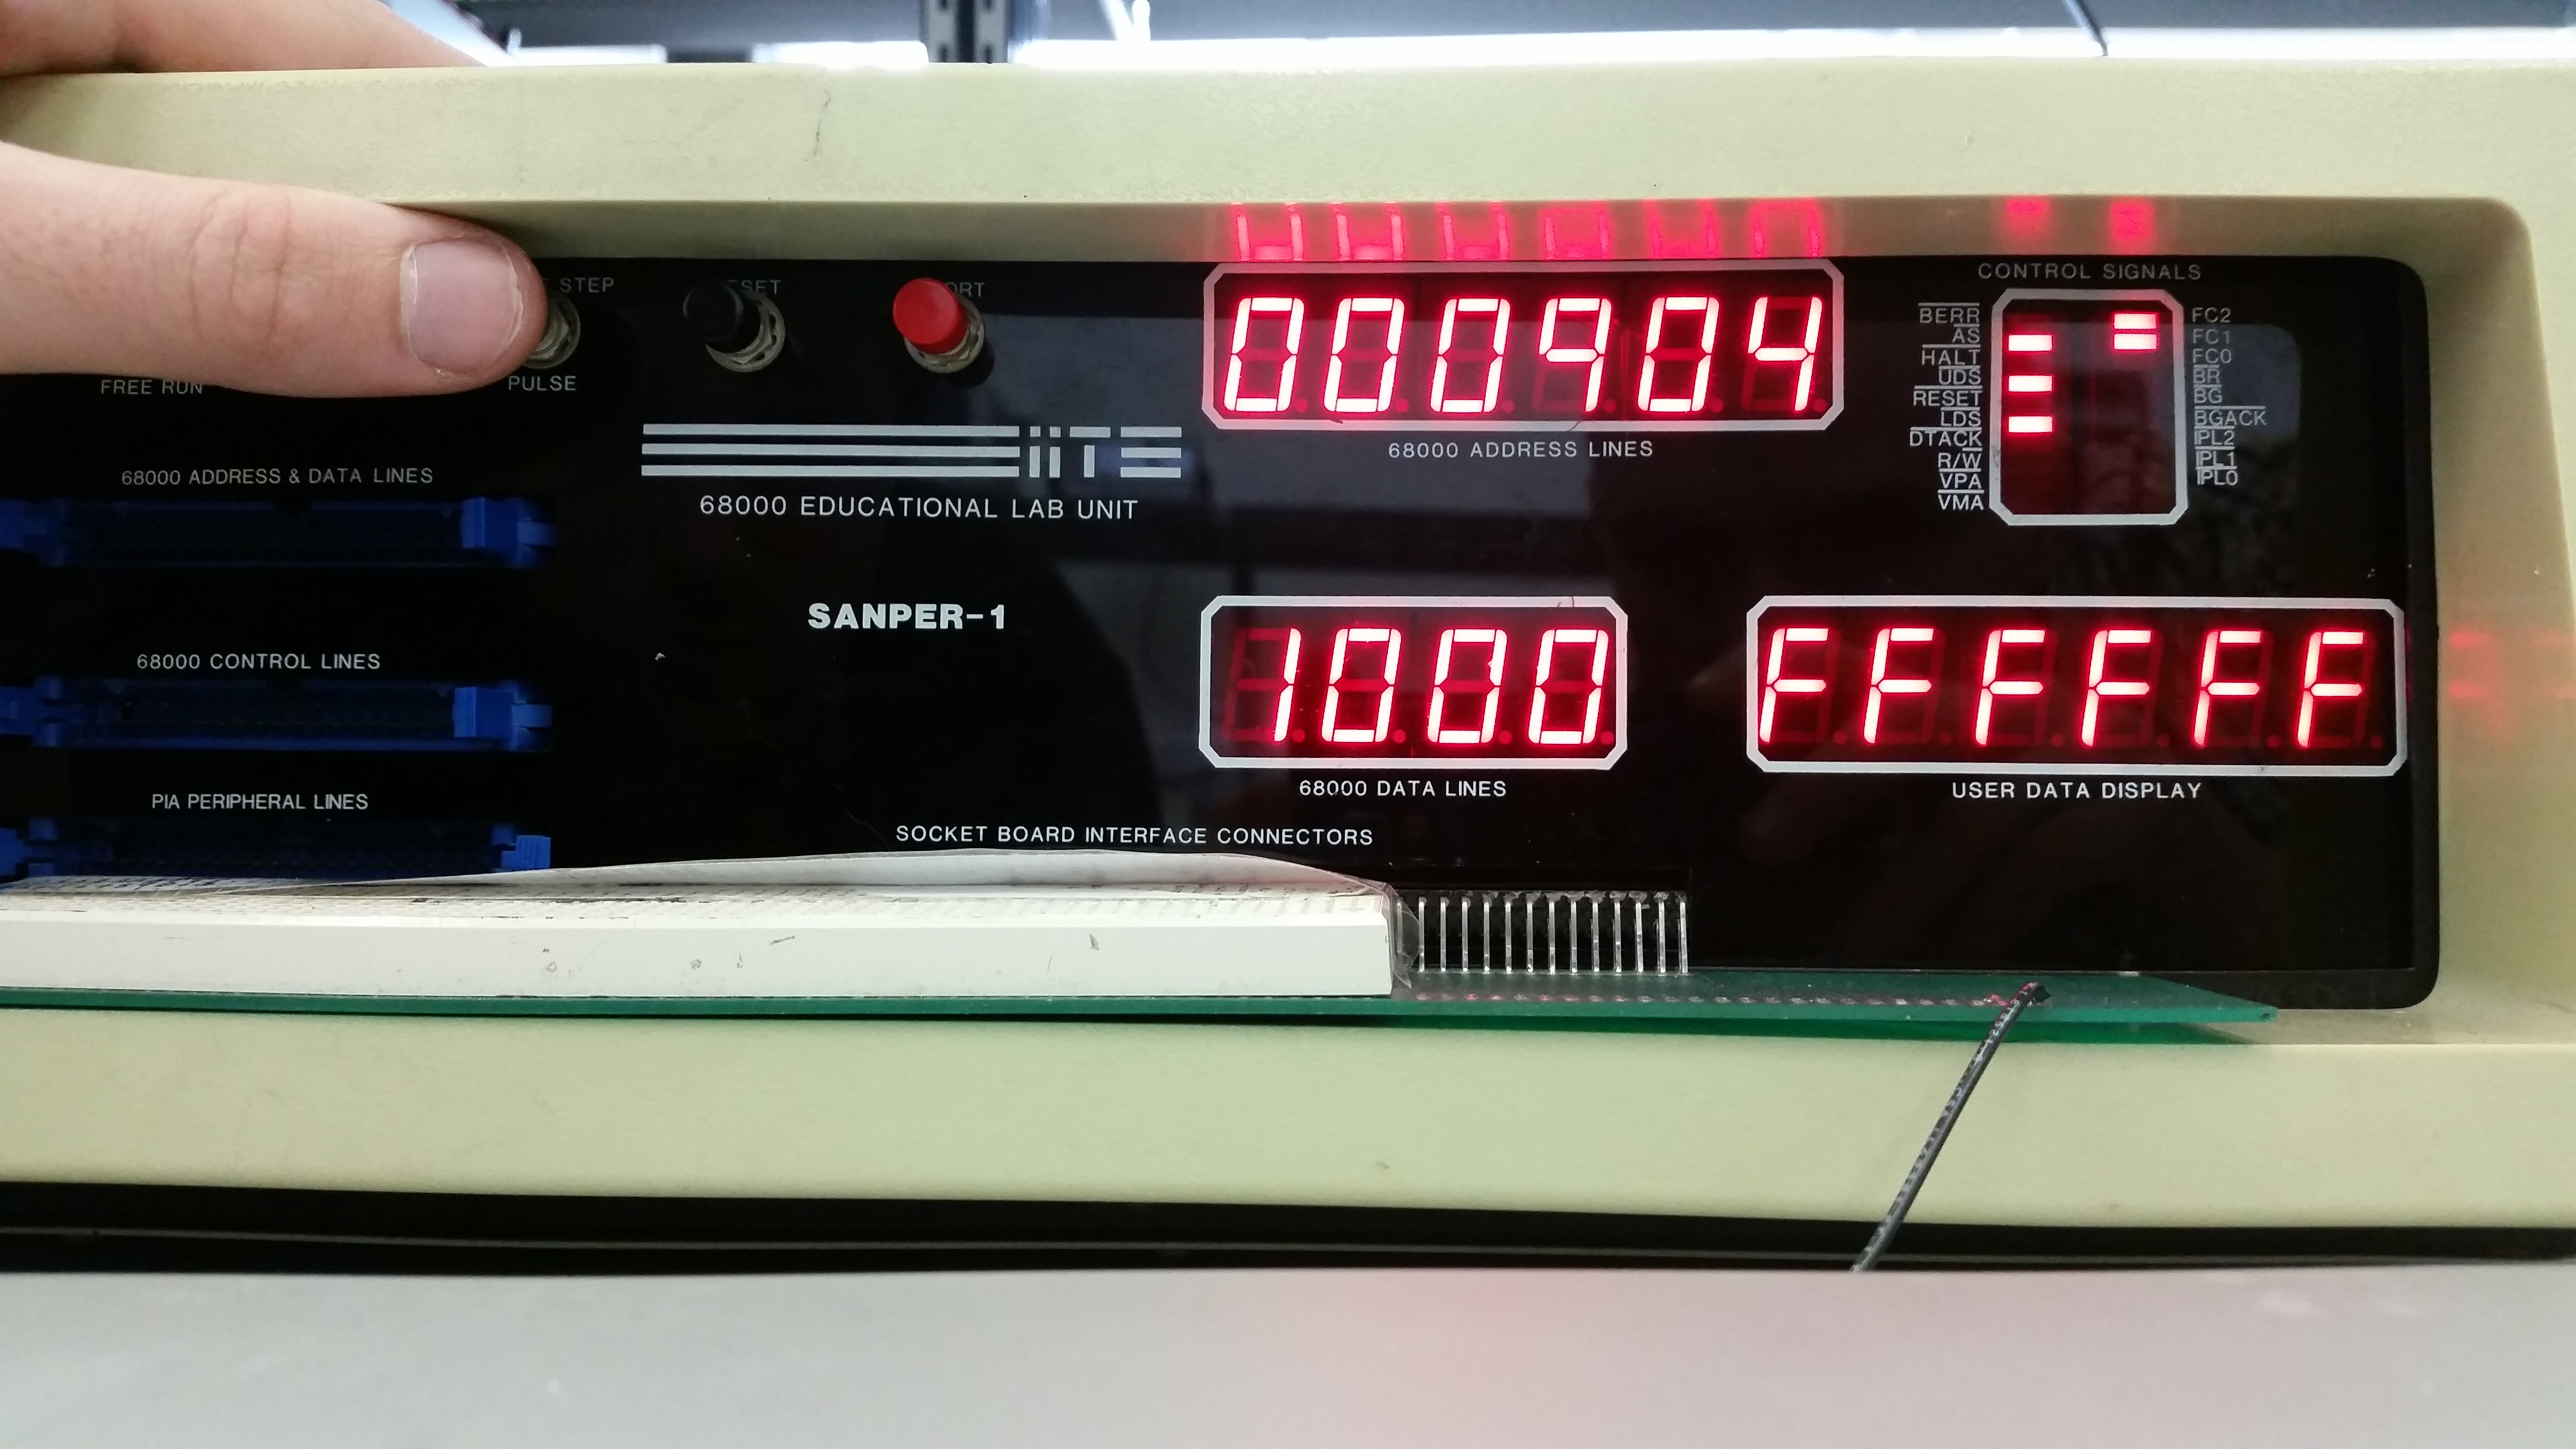
\includegraphics[width=1\linewidth]{Lab1/20150120_094838}
\end{center}
\begin{center}
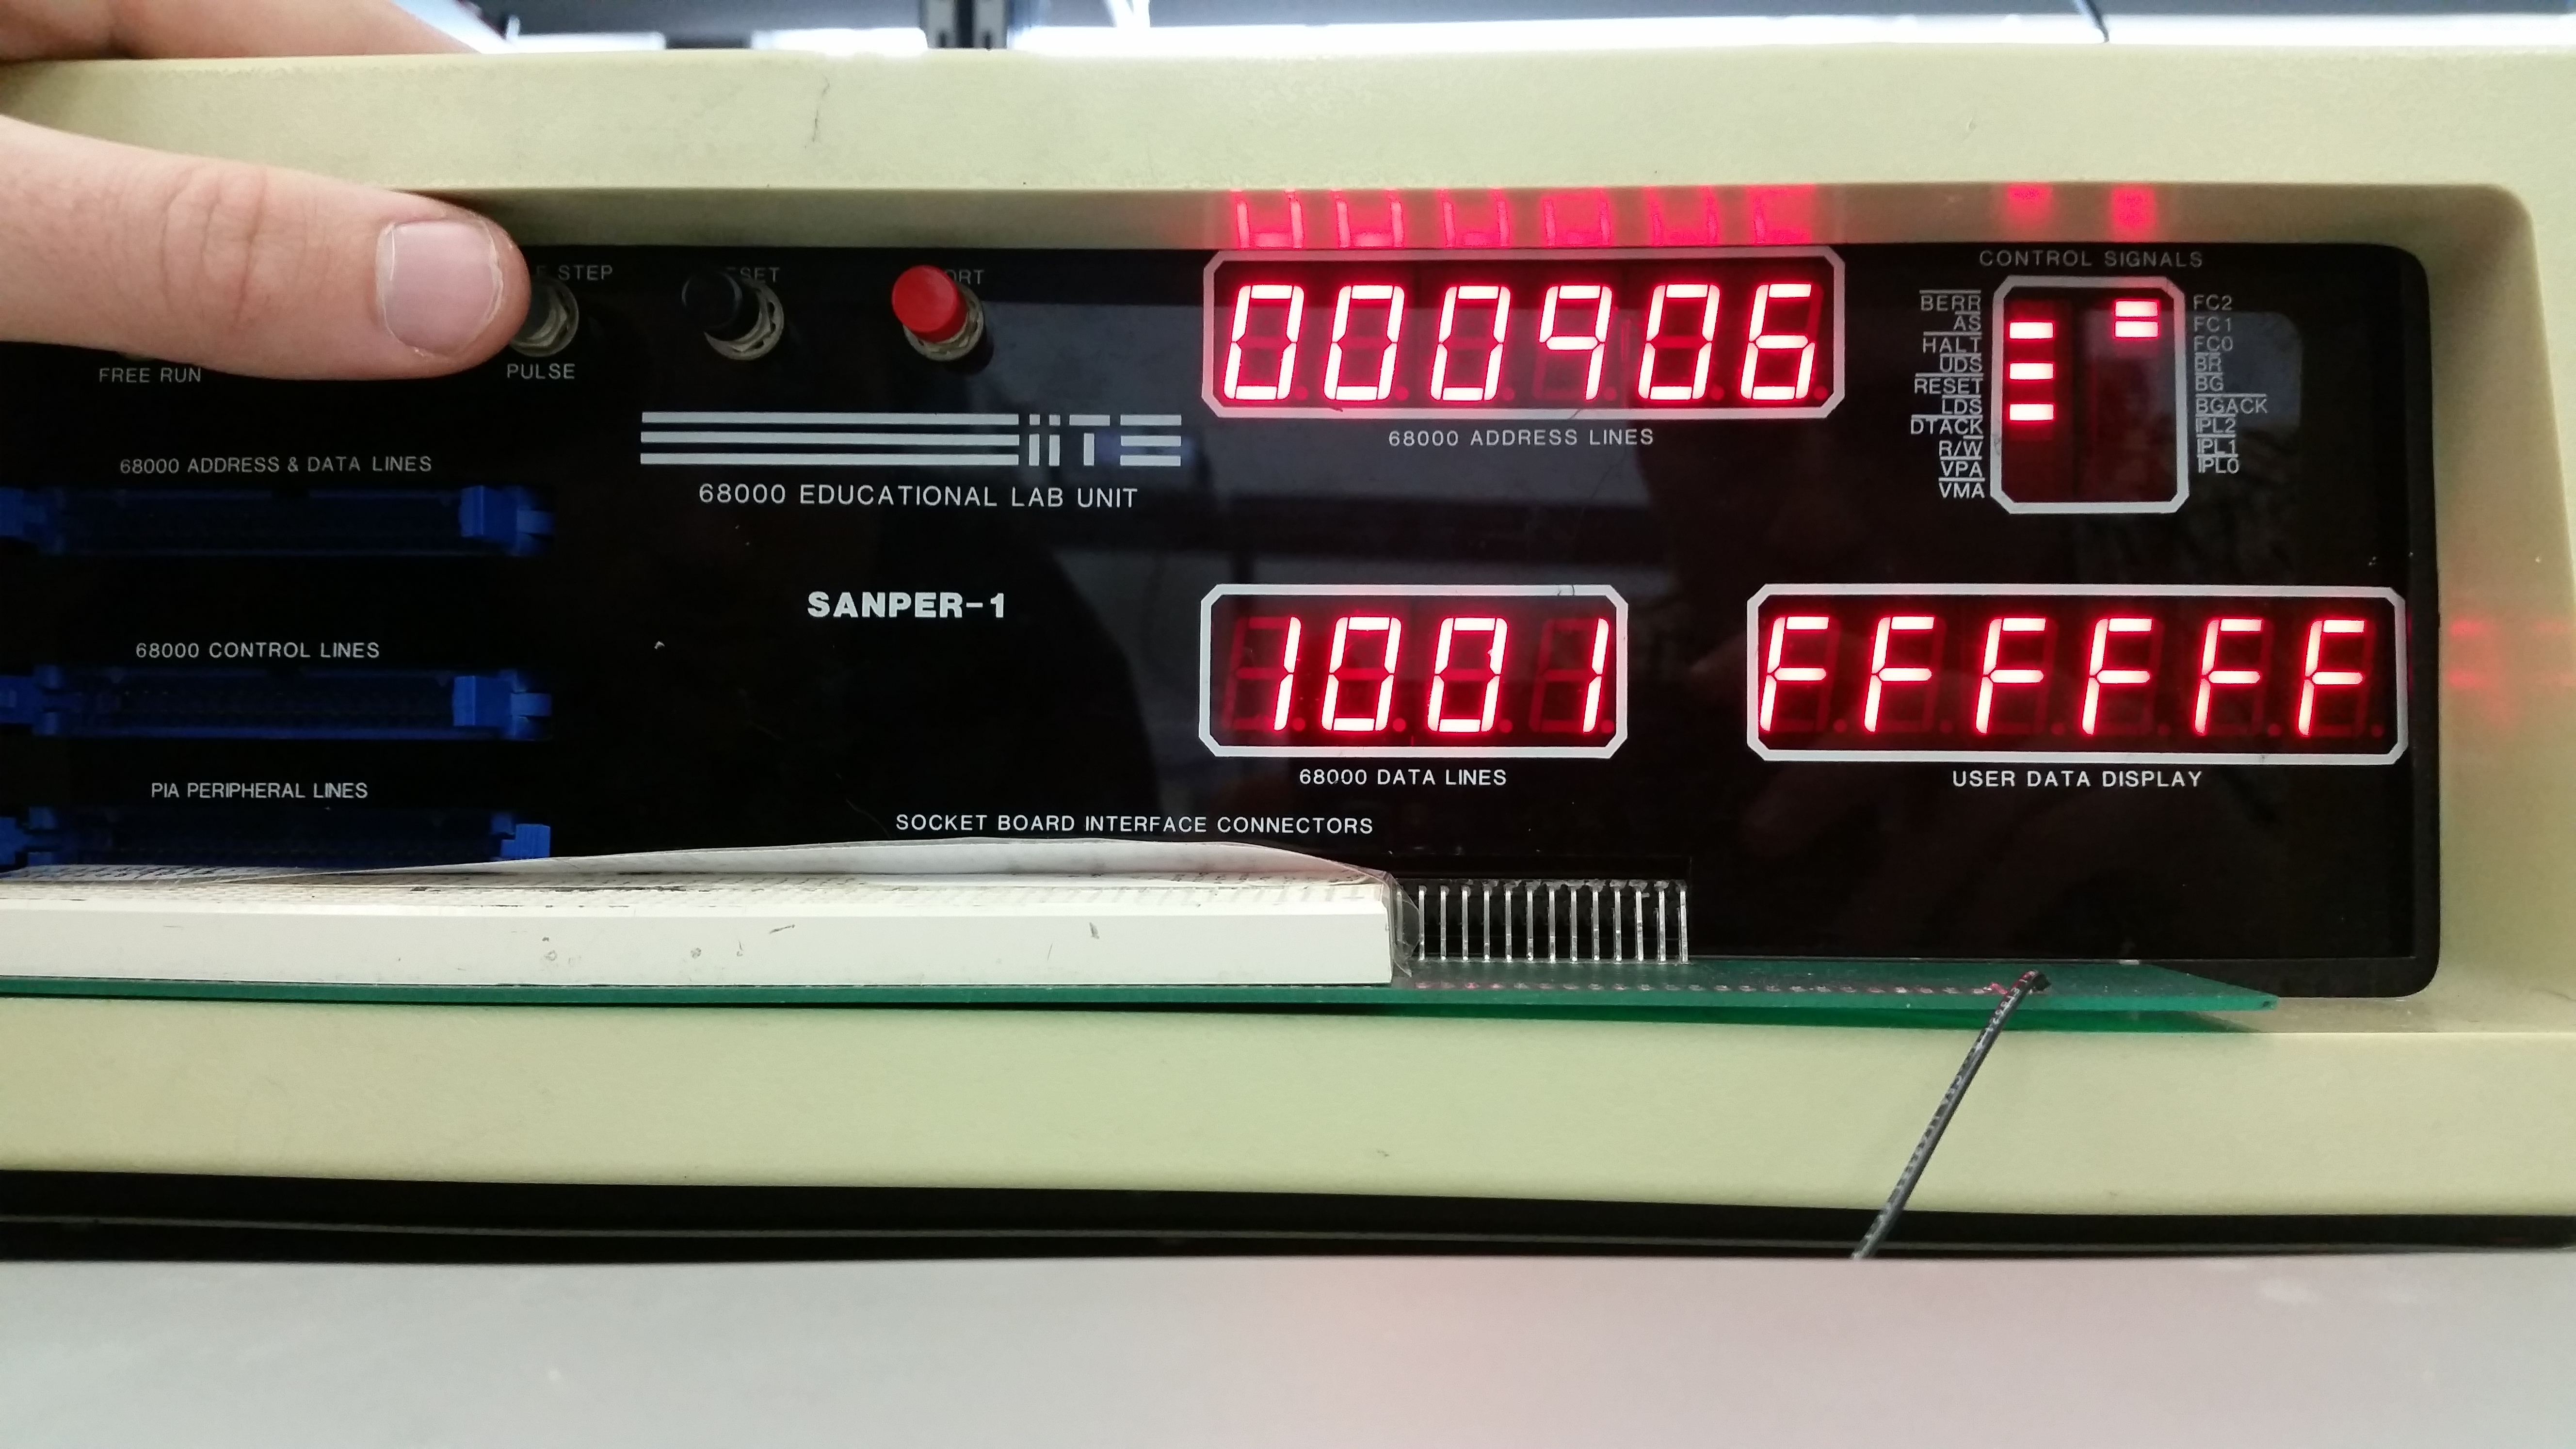
\includegraphics[width=1\linewidth]{Lab1/20150120_094840}
\end{center}
\begin{center}
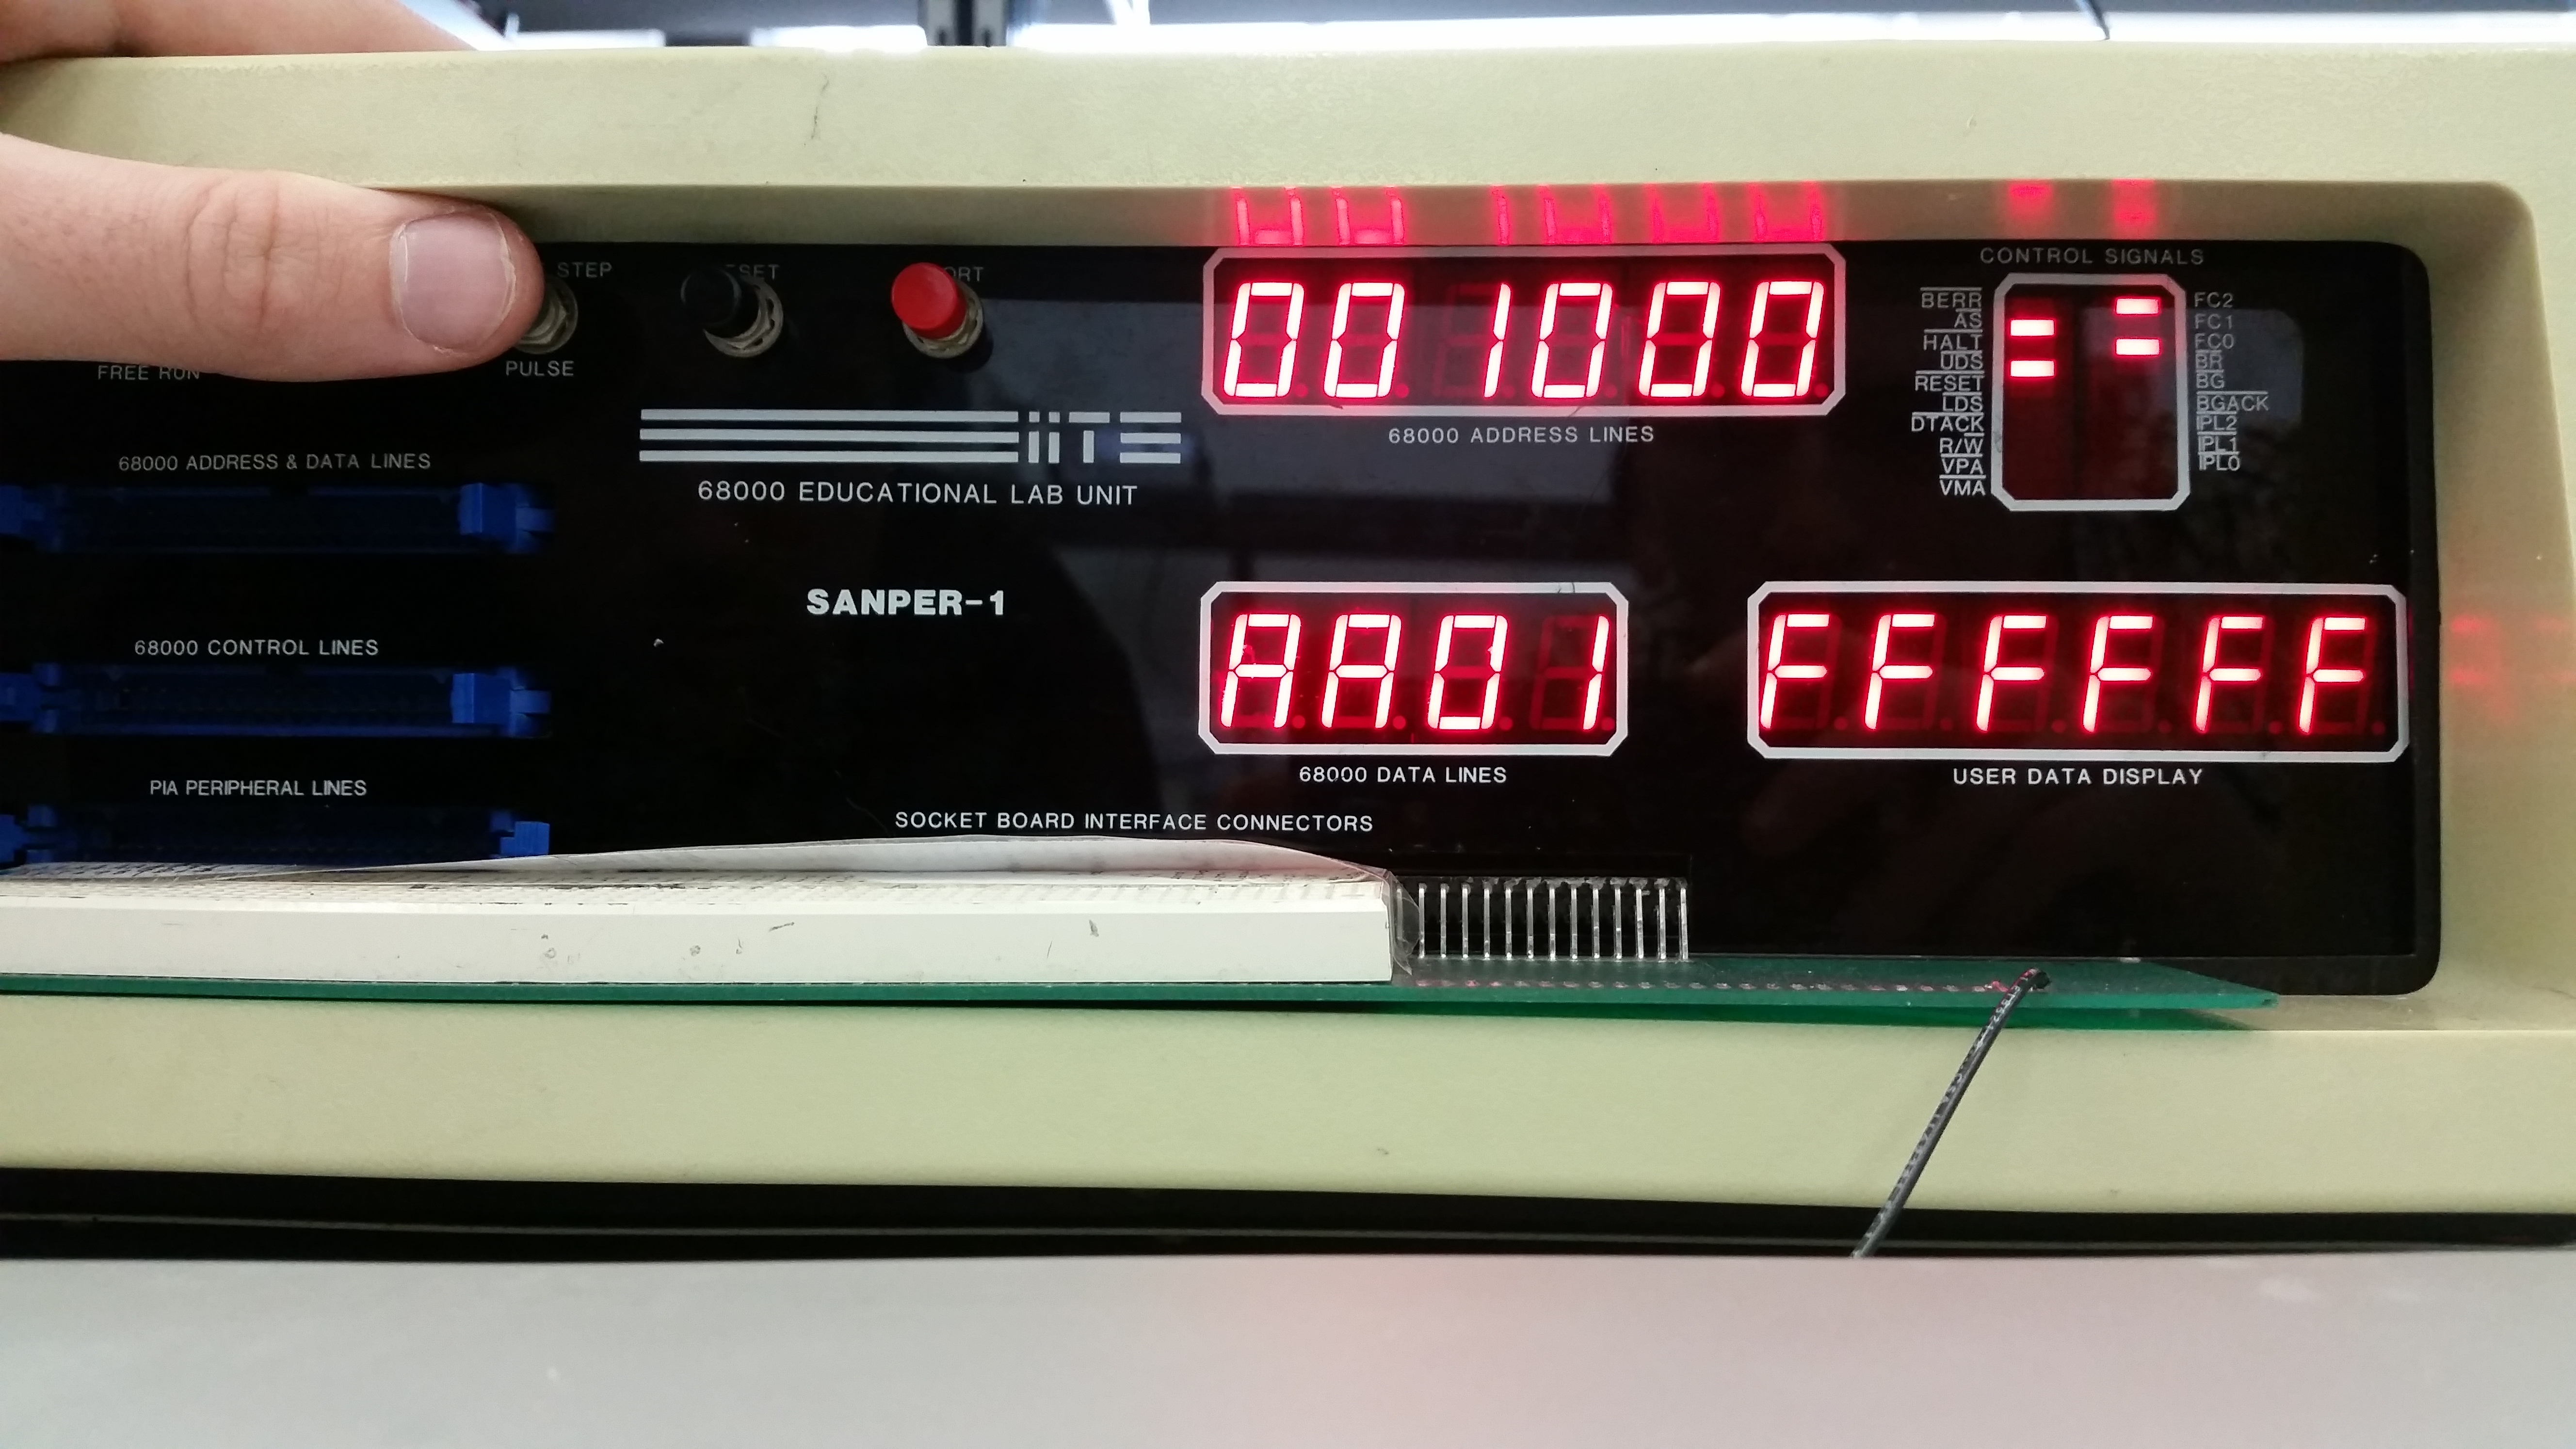
\includegraphics[width=1\linewidth]{Lab1/20150120_094841}
\end{center}
\begin{center}
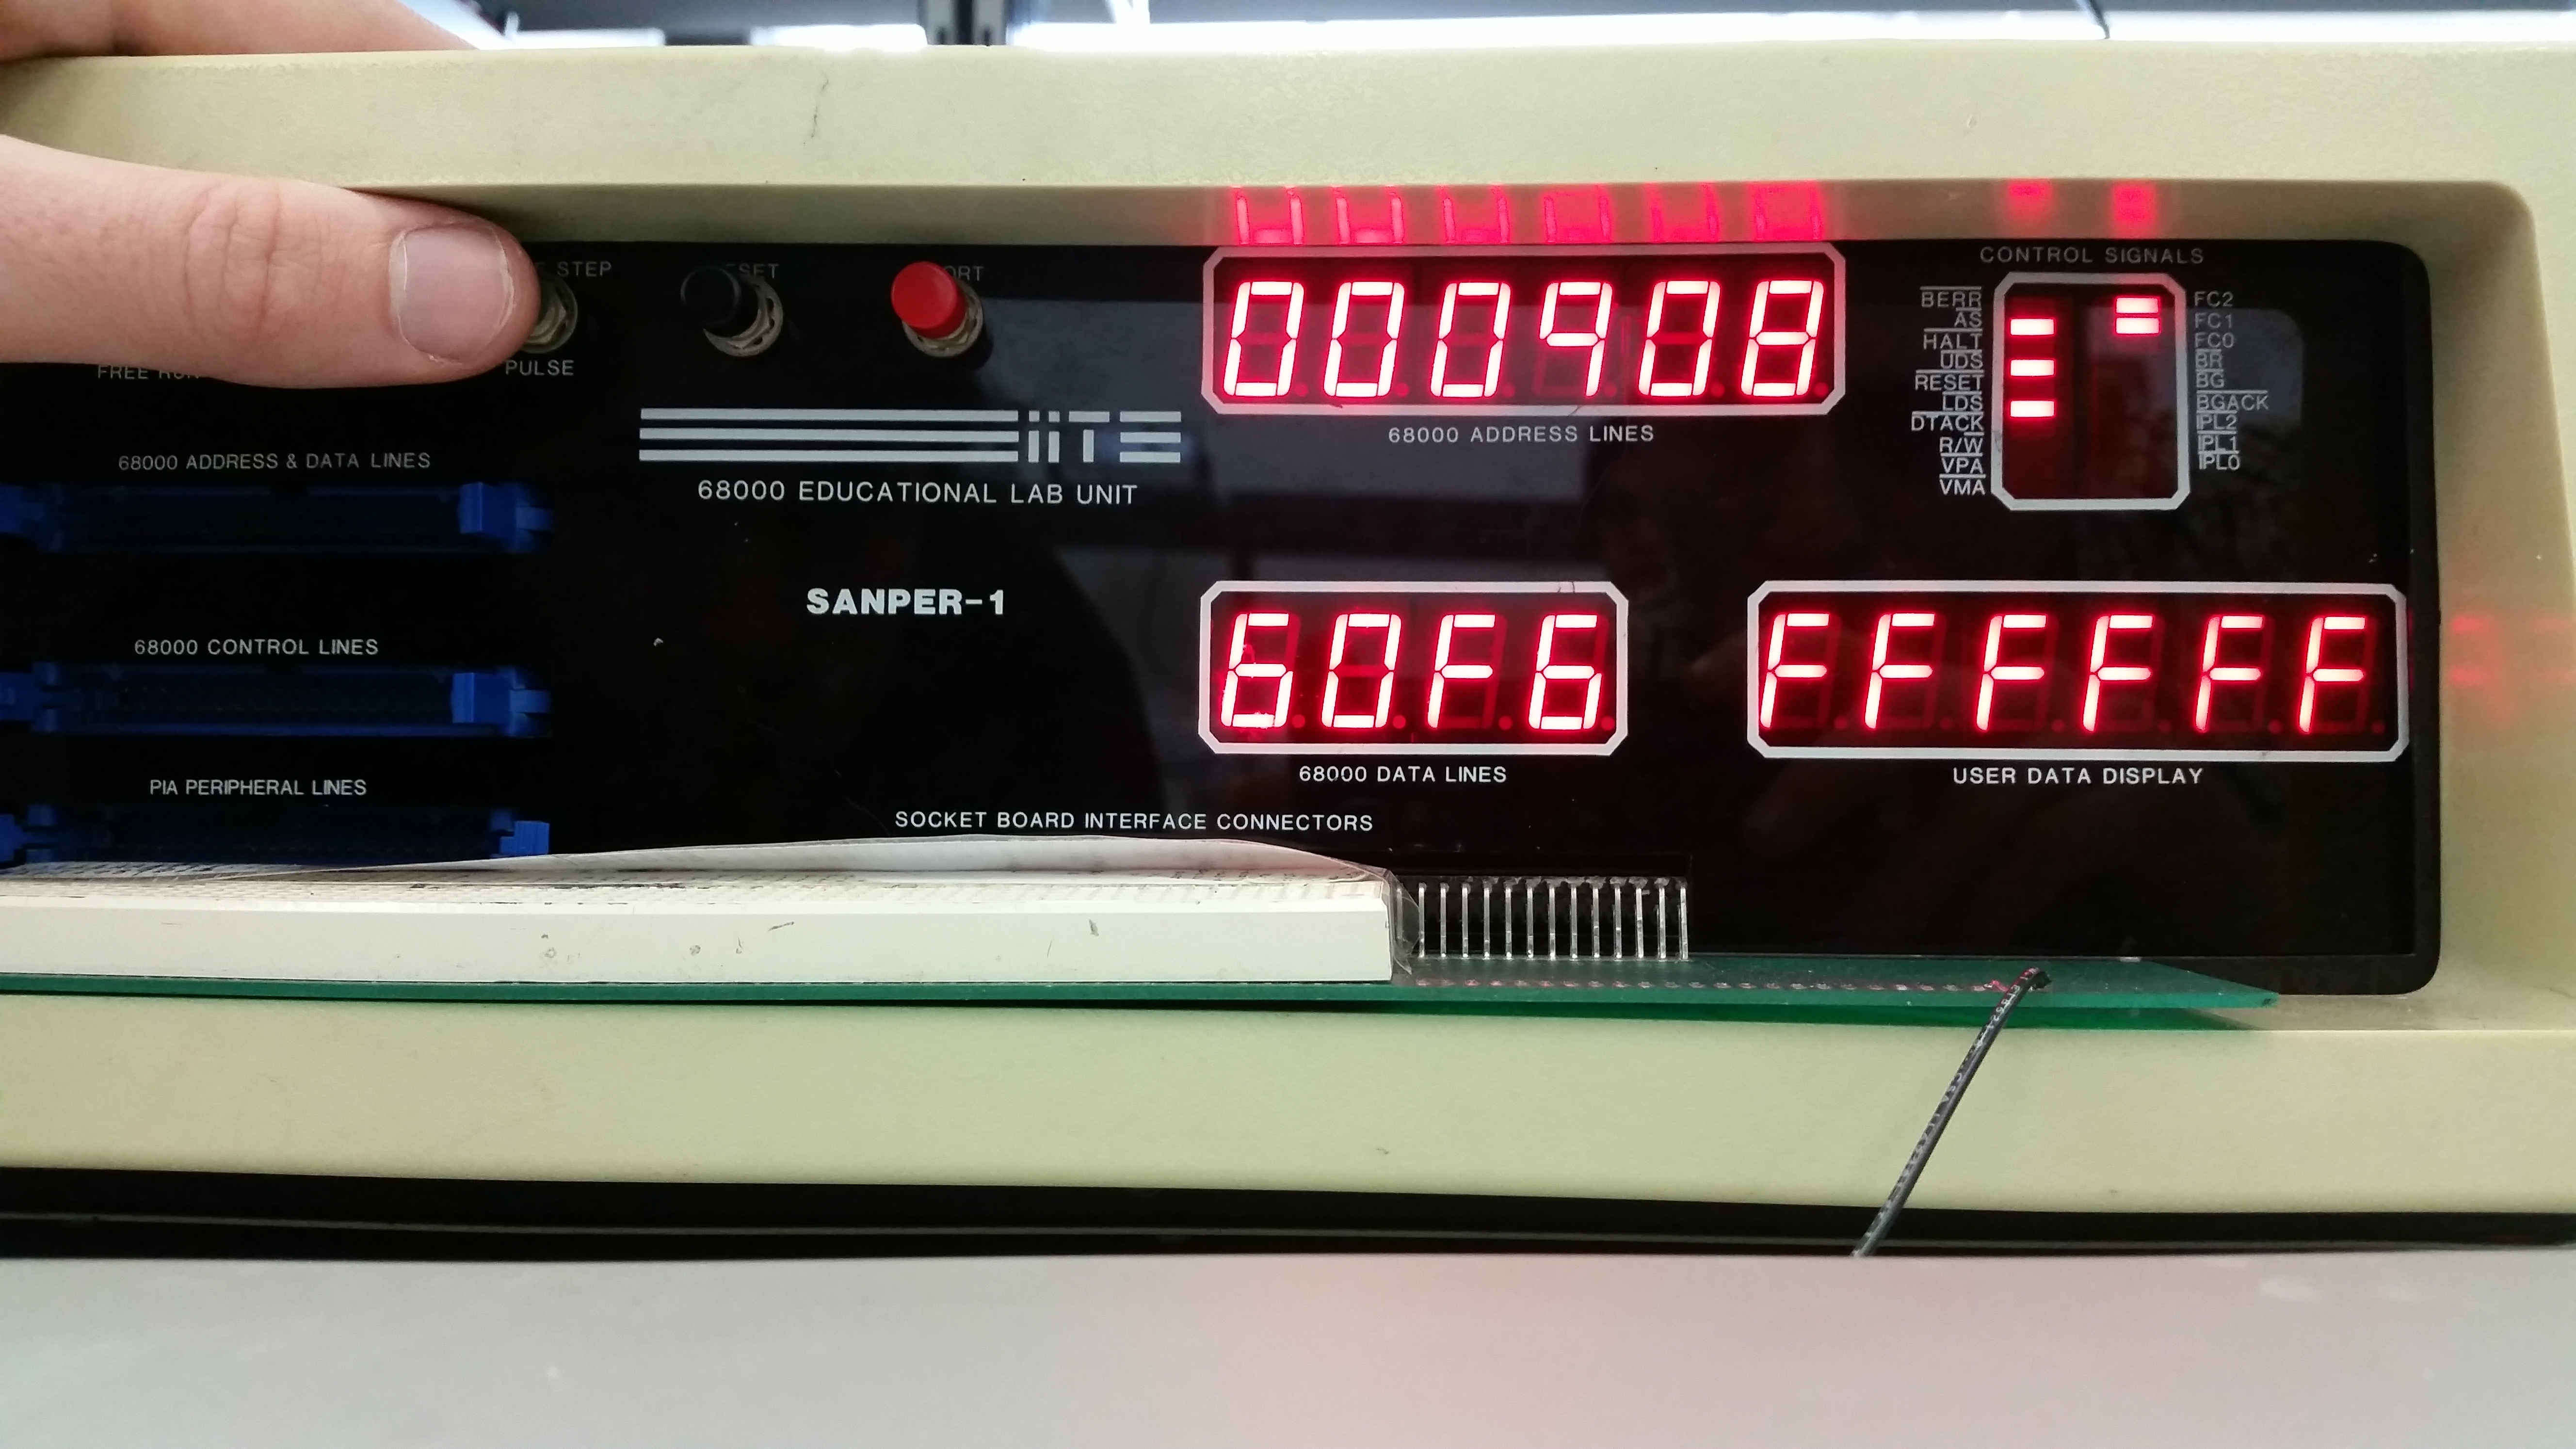
\includegraphics[width=1\linewidth]{Lab1/20150120_094843}
\end{center}
\begin{center}
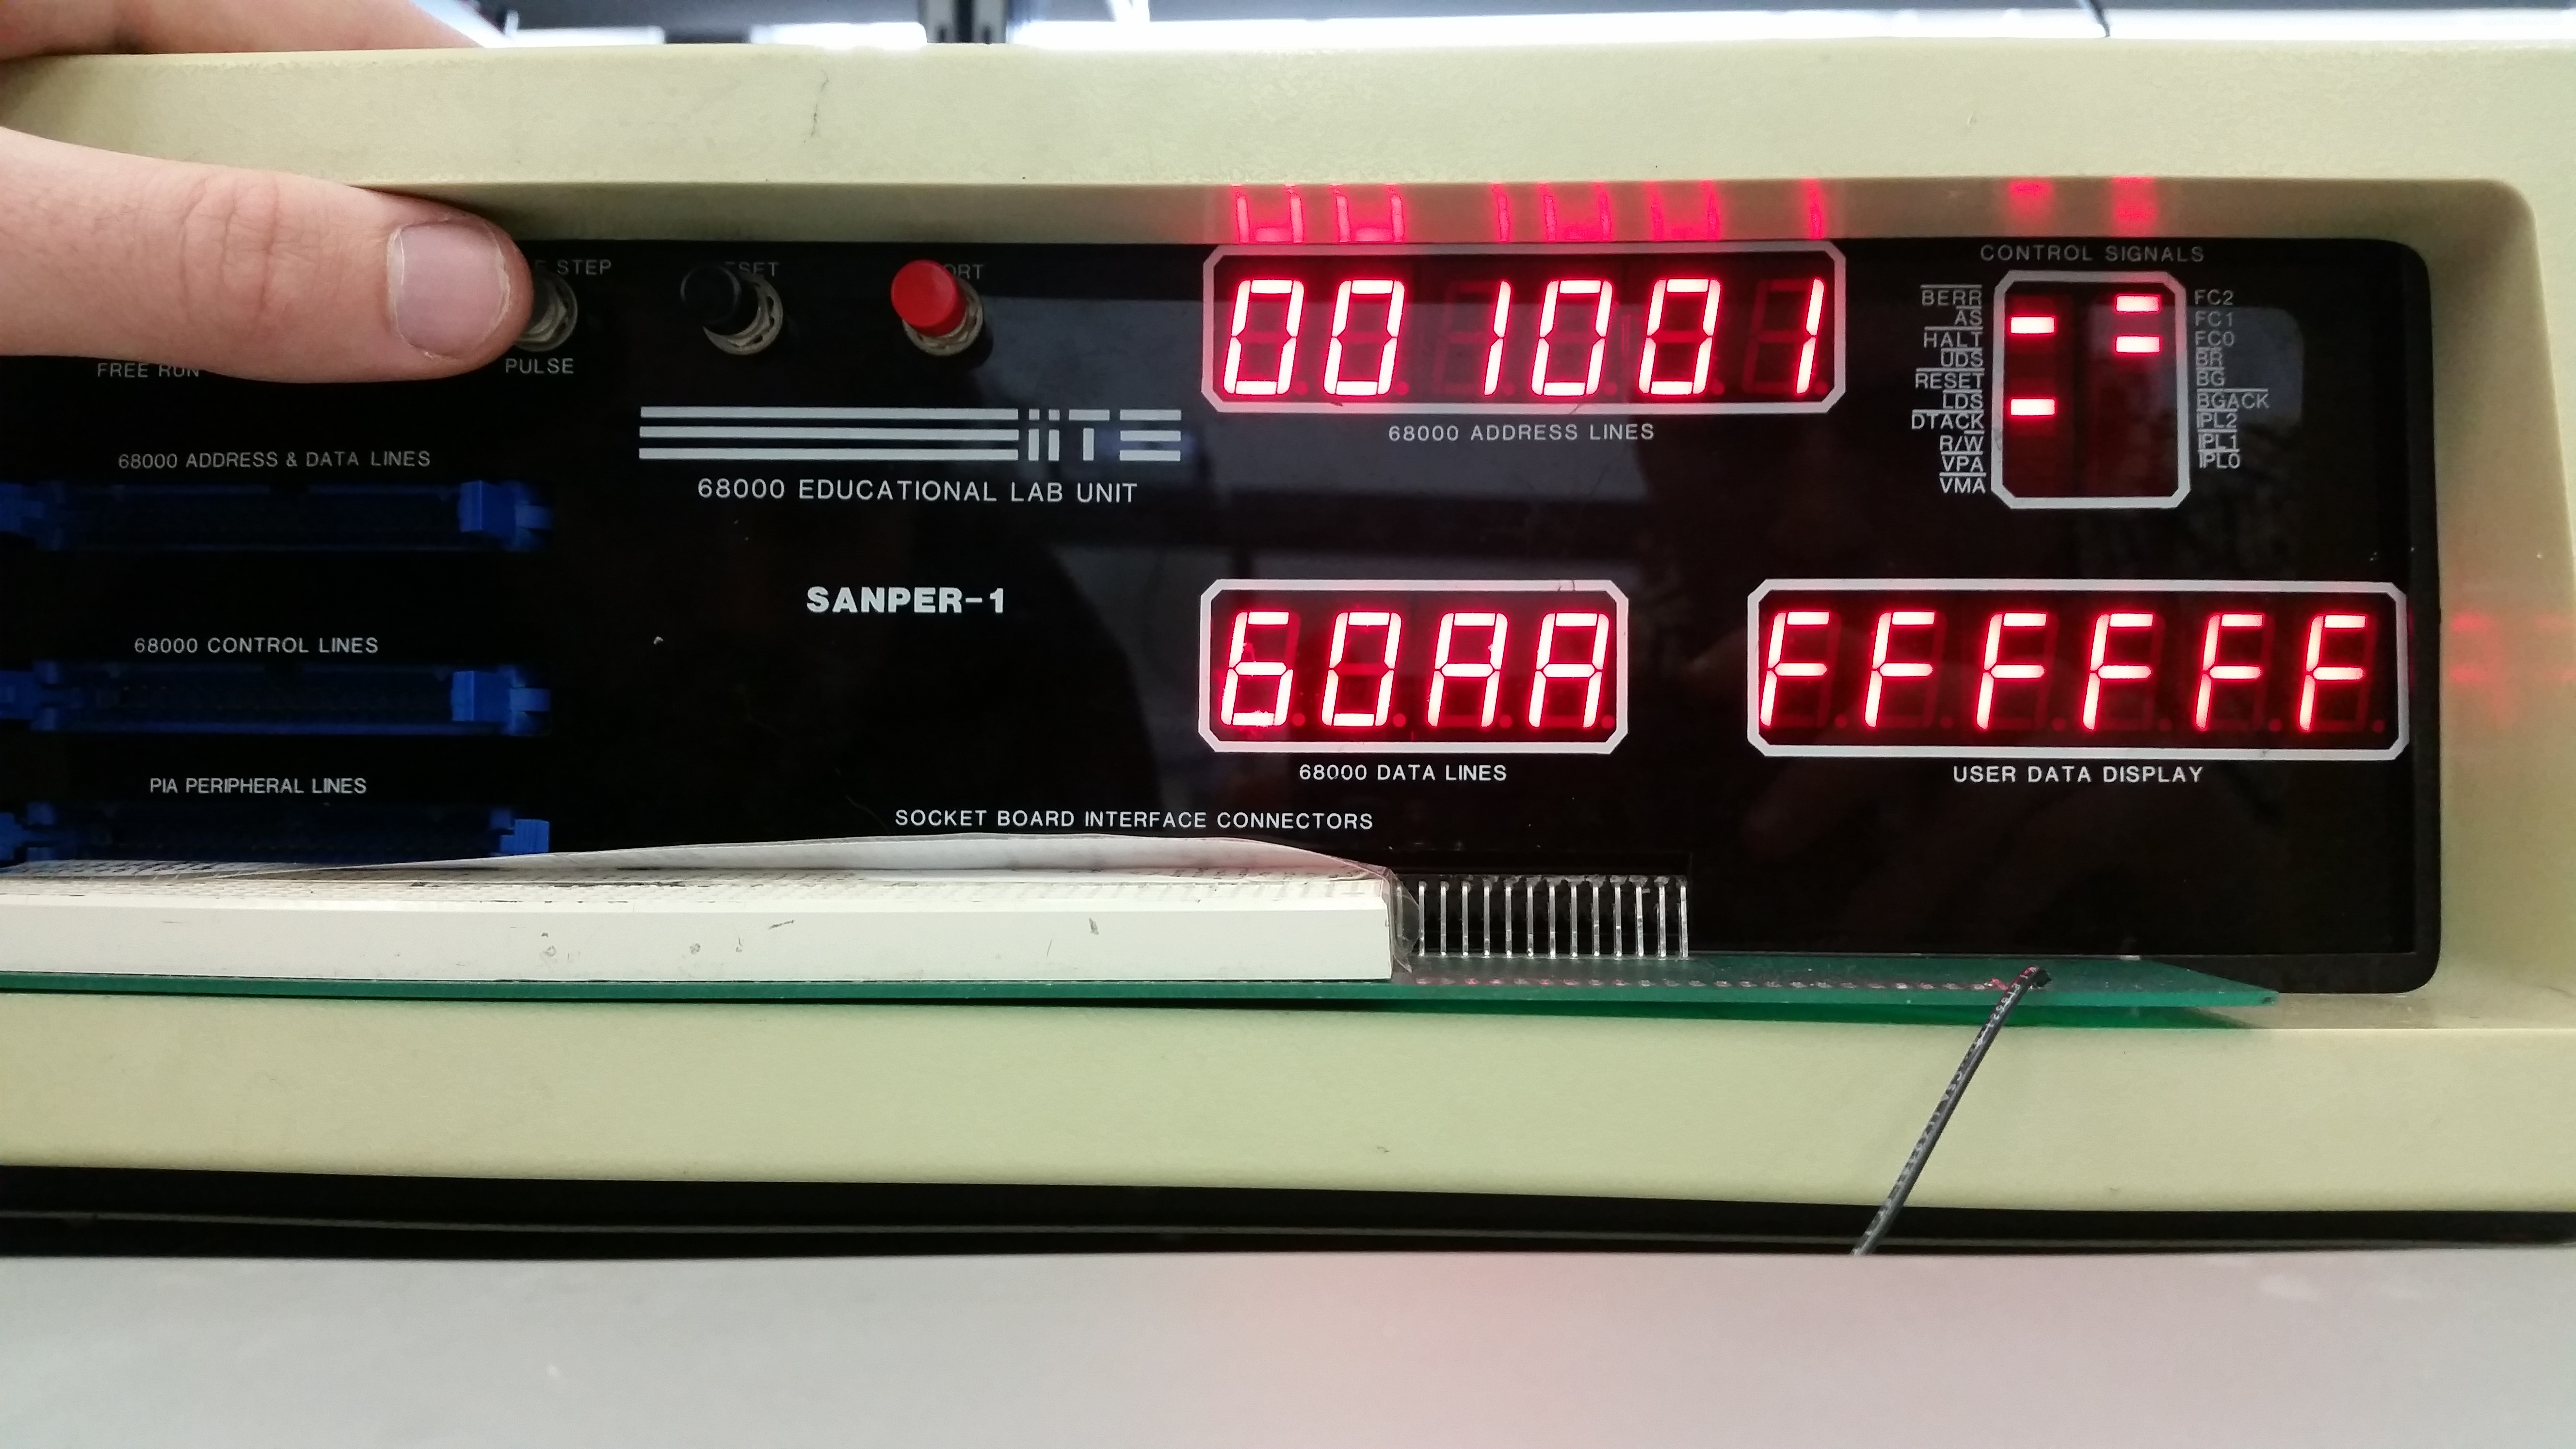
\includegraphics[width=1\linewidth]{Lab1/20150120_094845}
\end{center}
\begin{center}
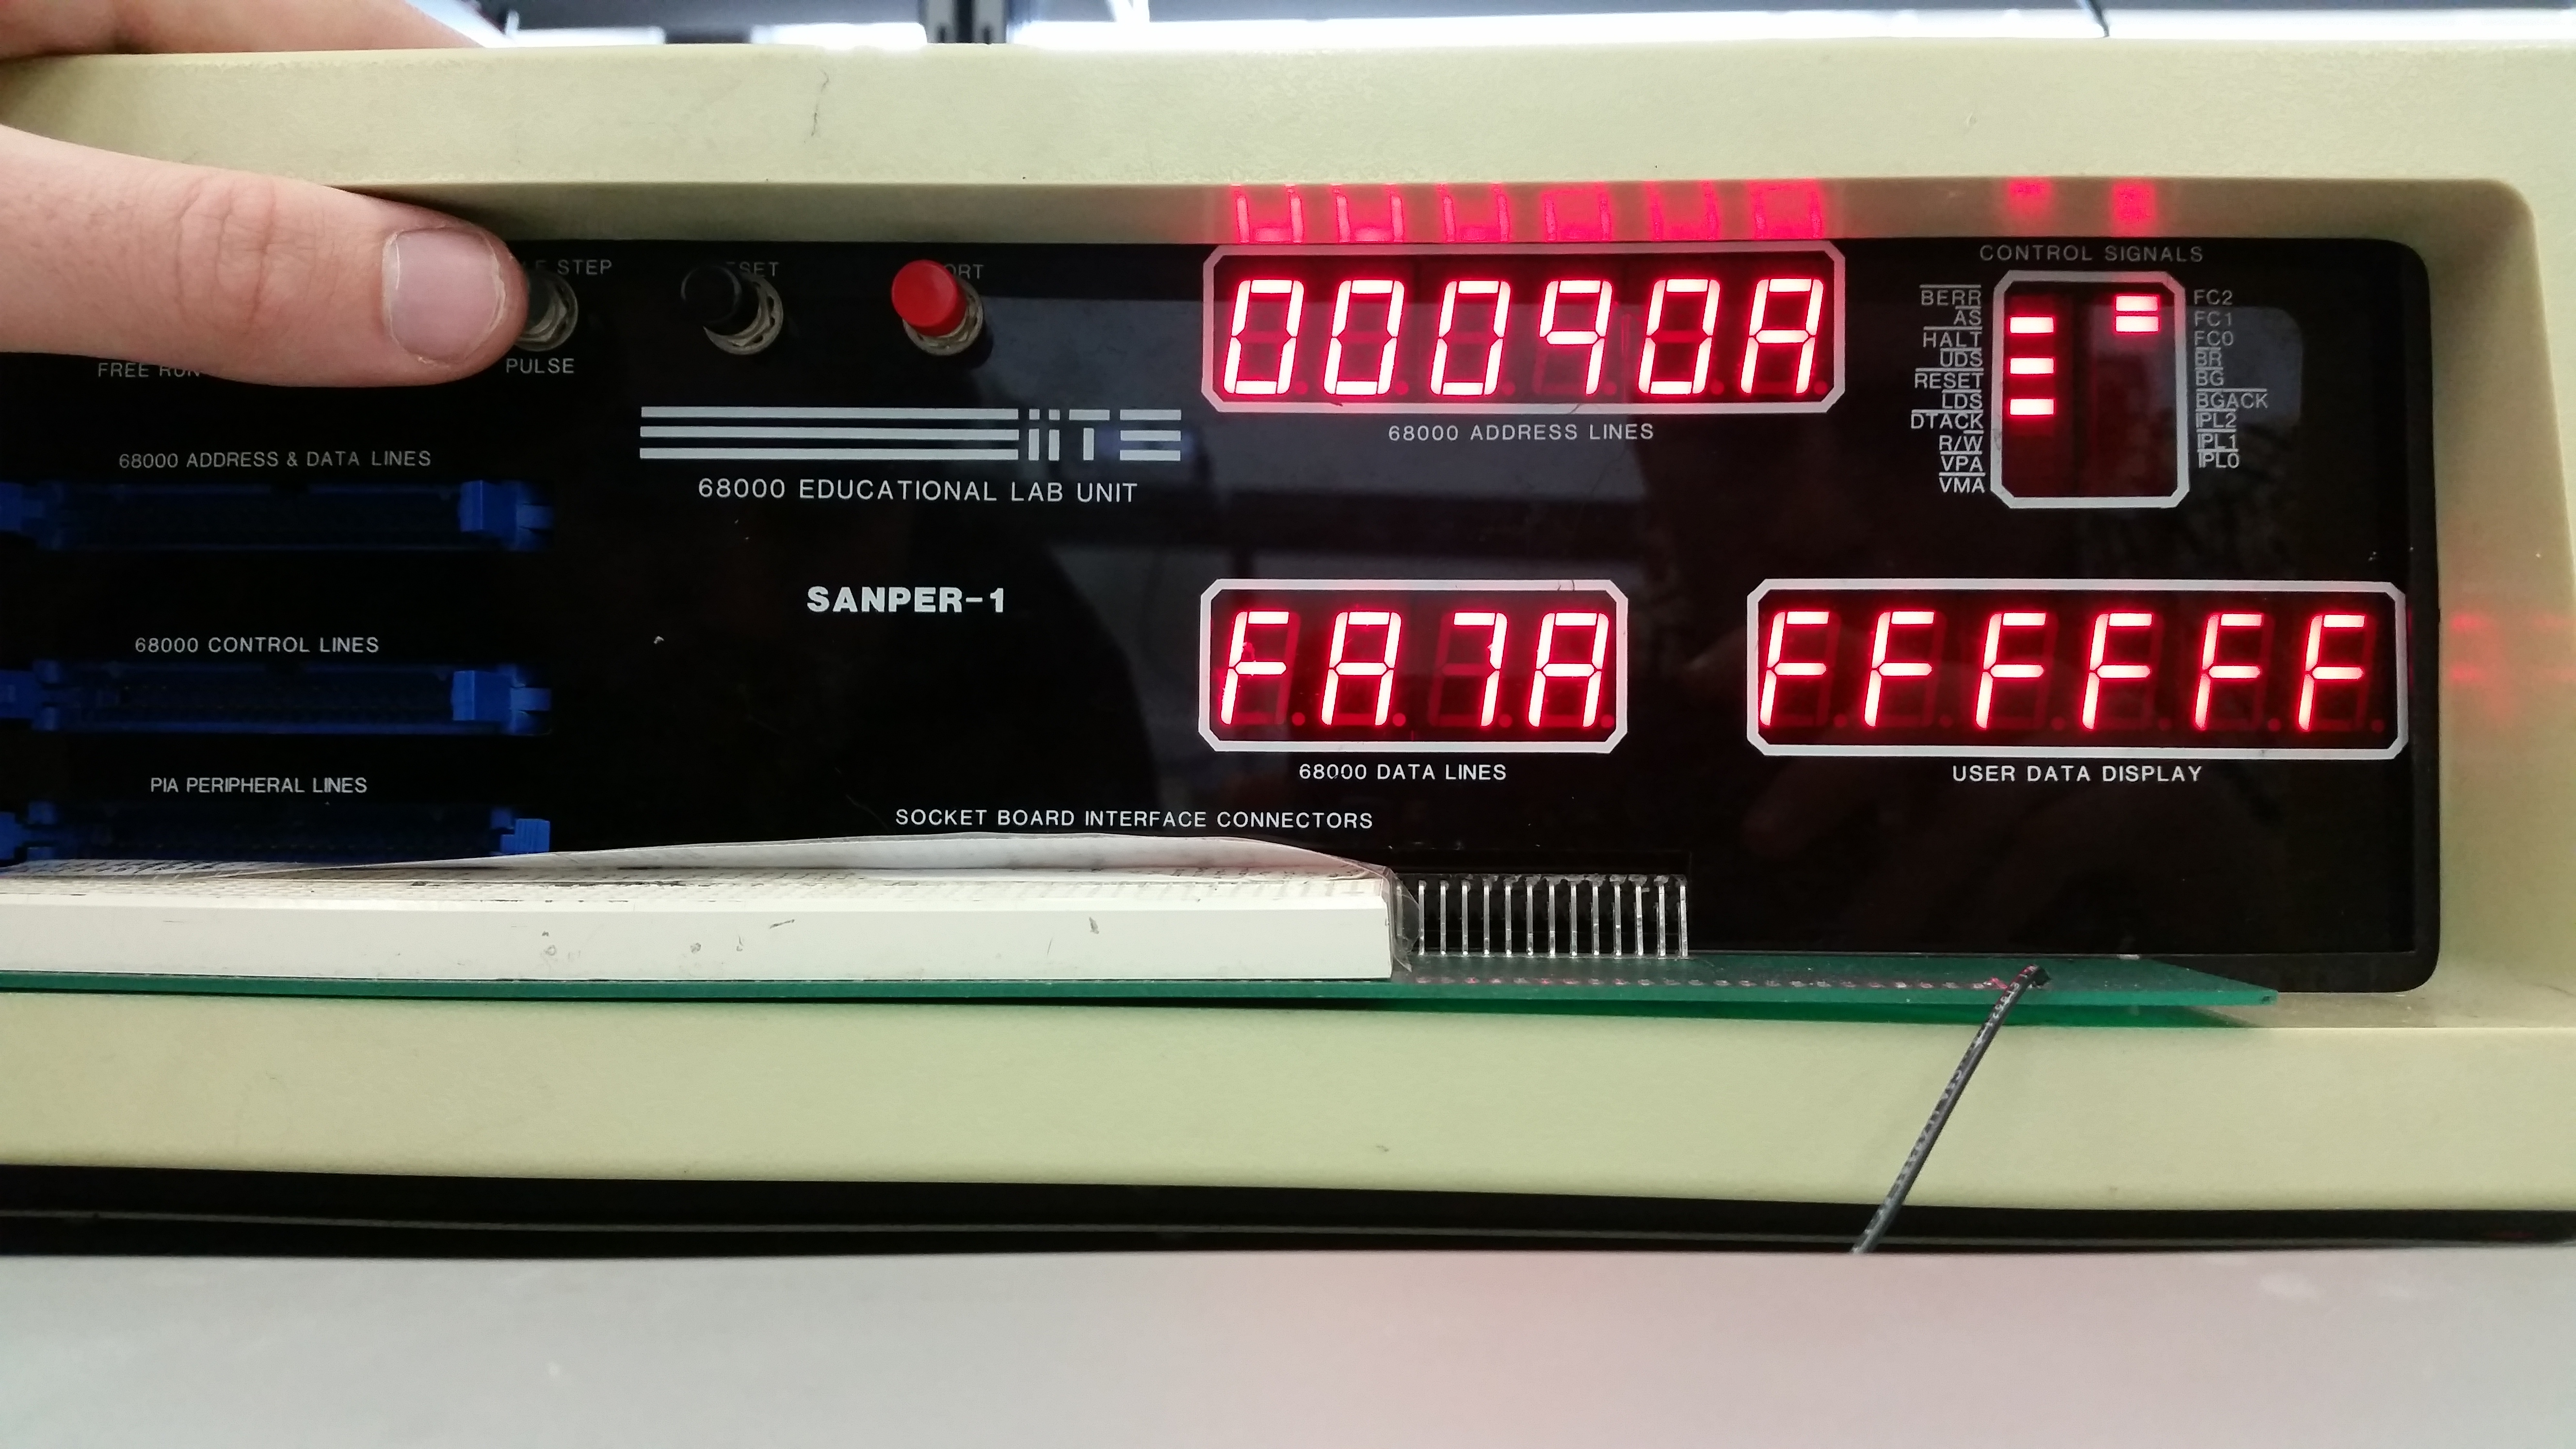
\includegraphics[width=1\linewidth]{Lab1/20150120_094847}
\end{center}
\begin{center}
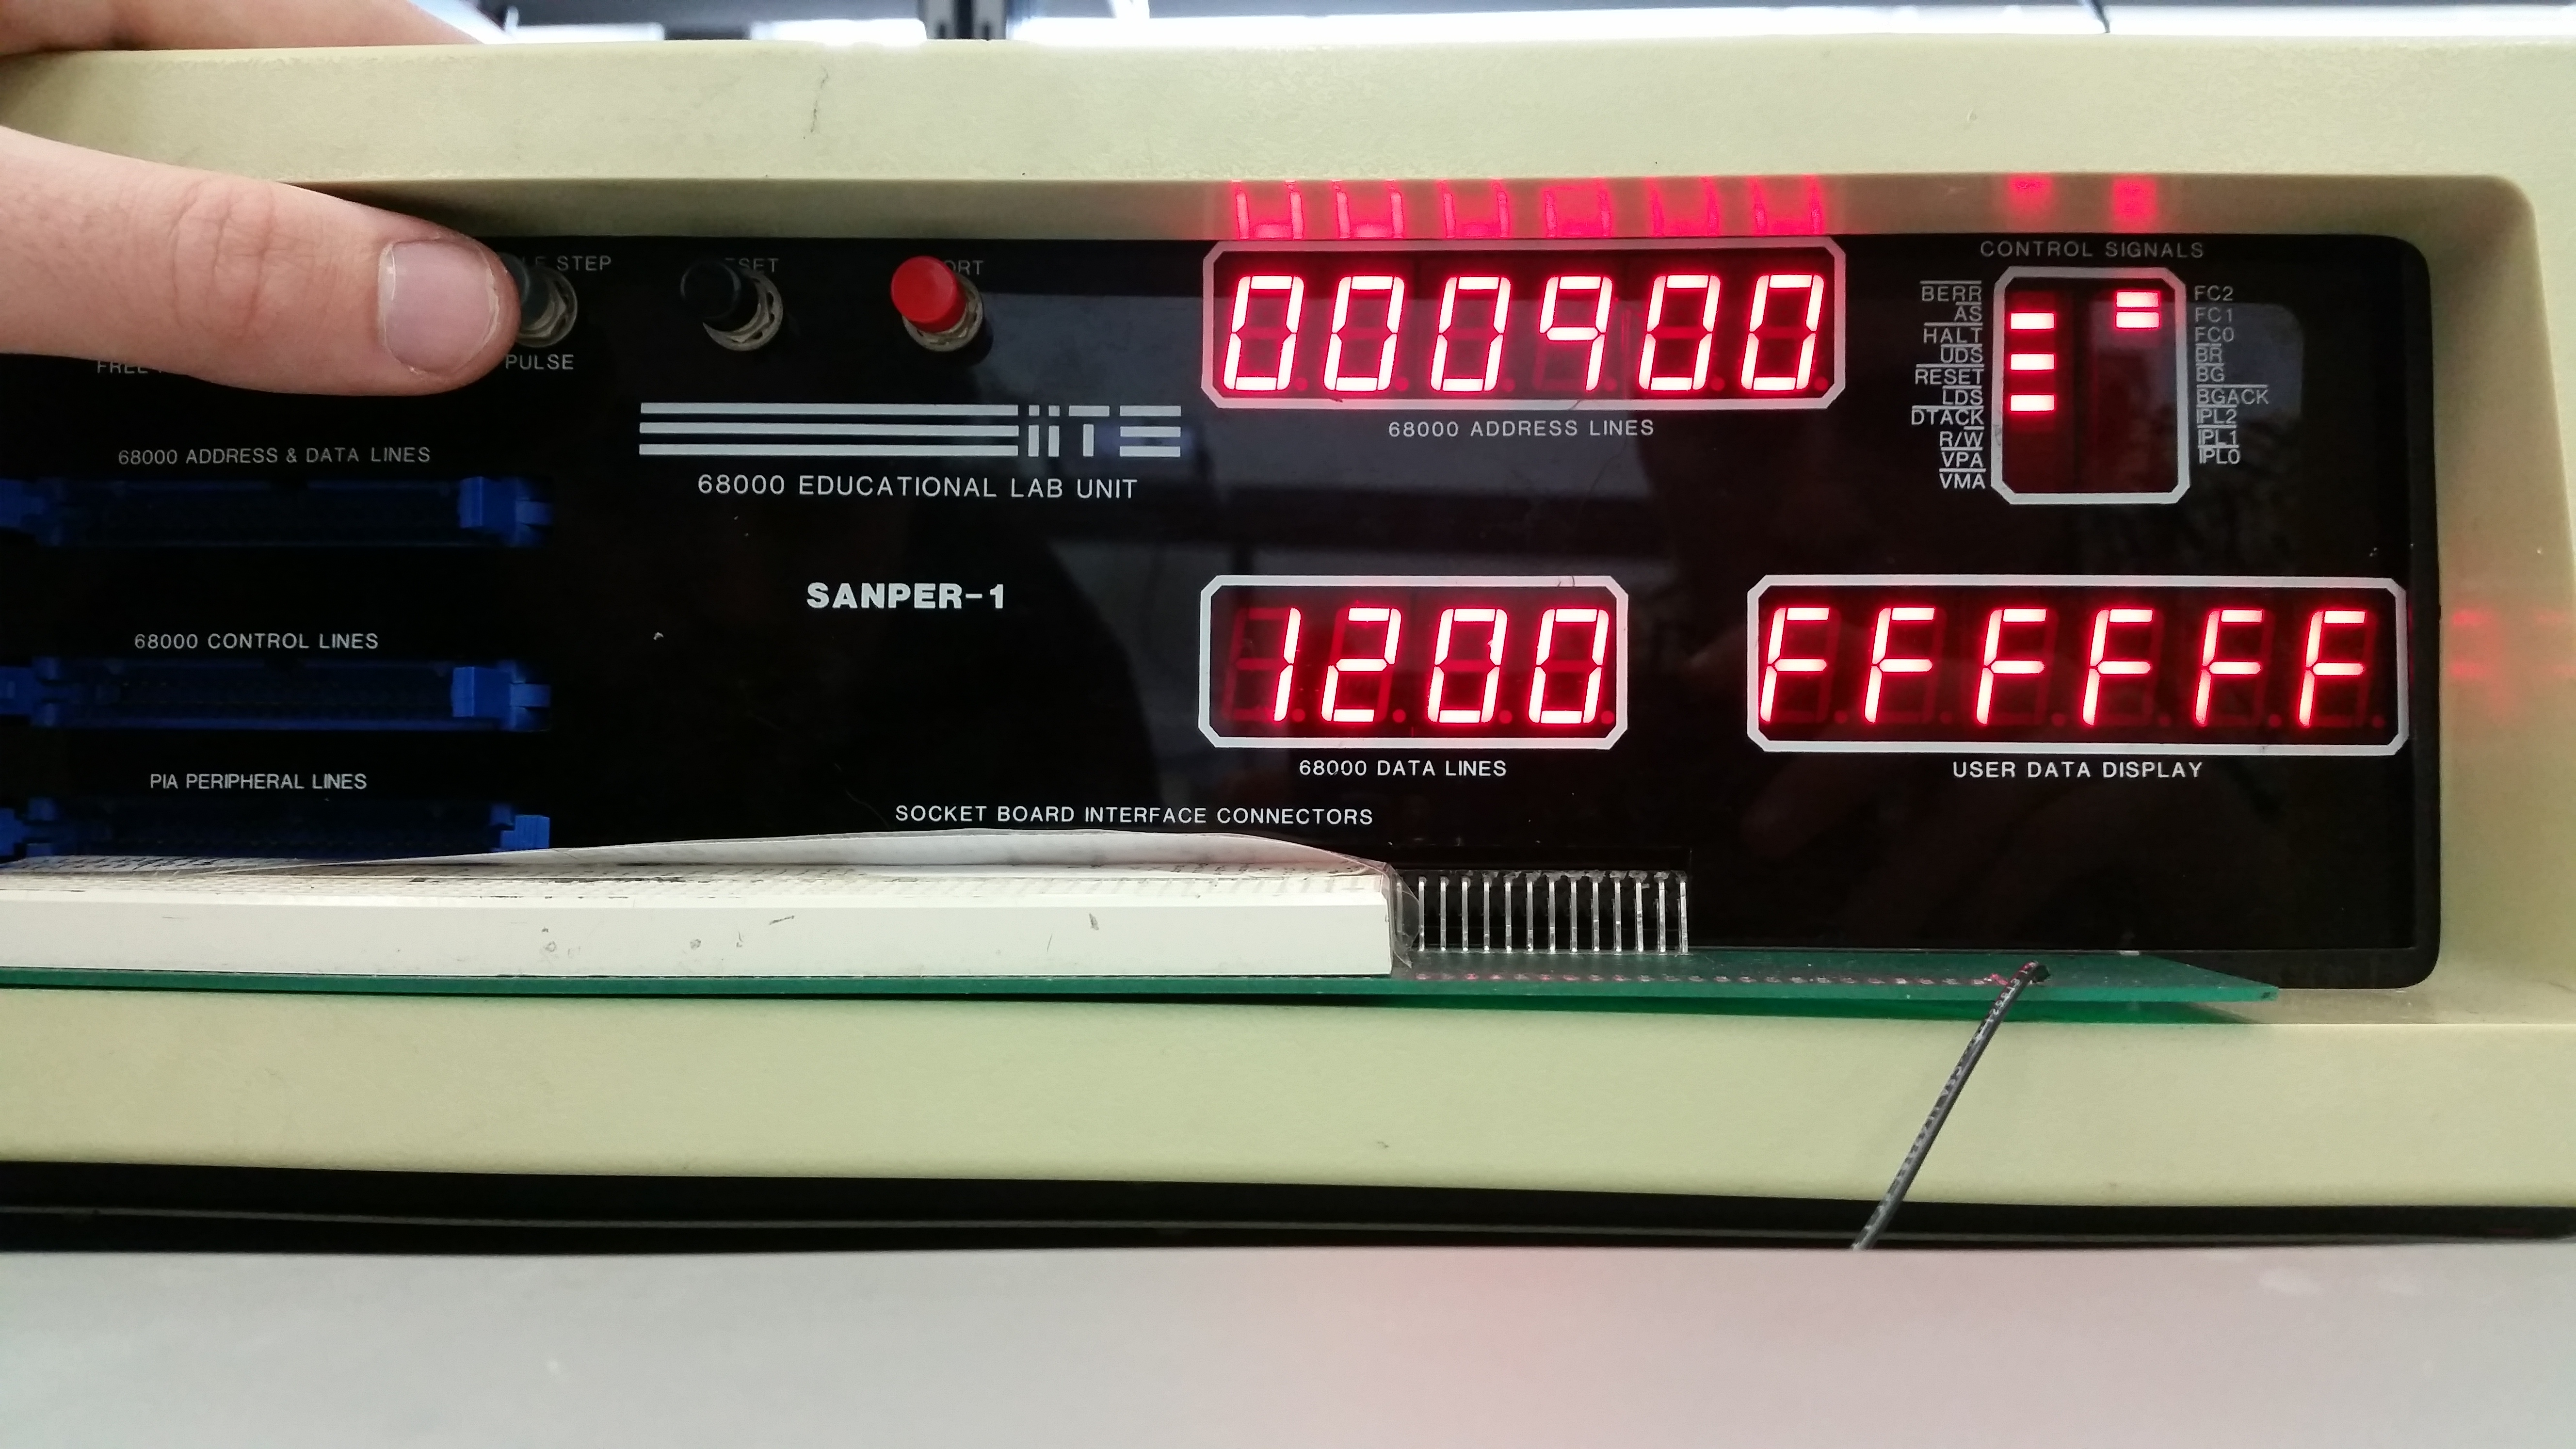
\includegraphics[width=1\linewidth]{Lab1/20150120_094849}
\end{center}
\subsubsection{Reset Hardware Single Step Mode}
\label{resetpic}
\begin{center}
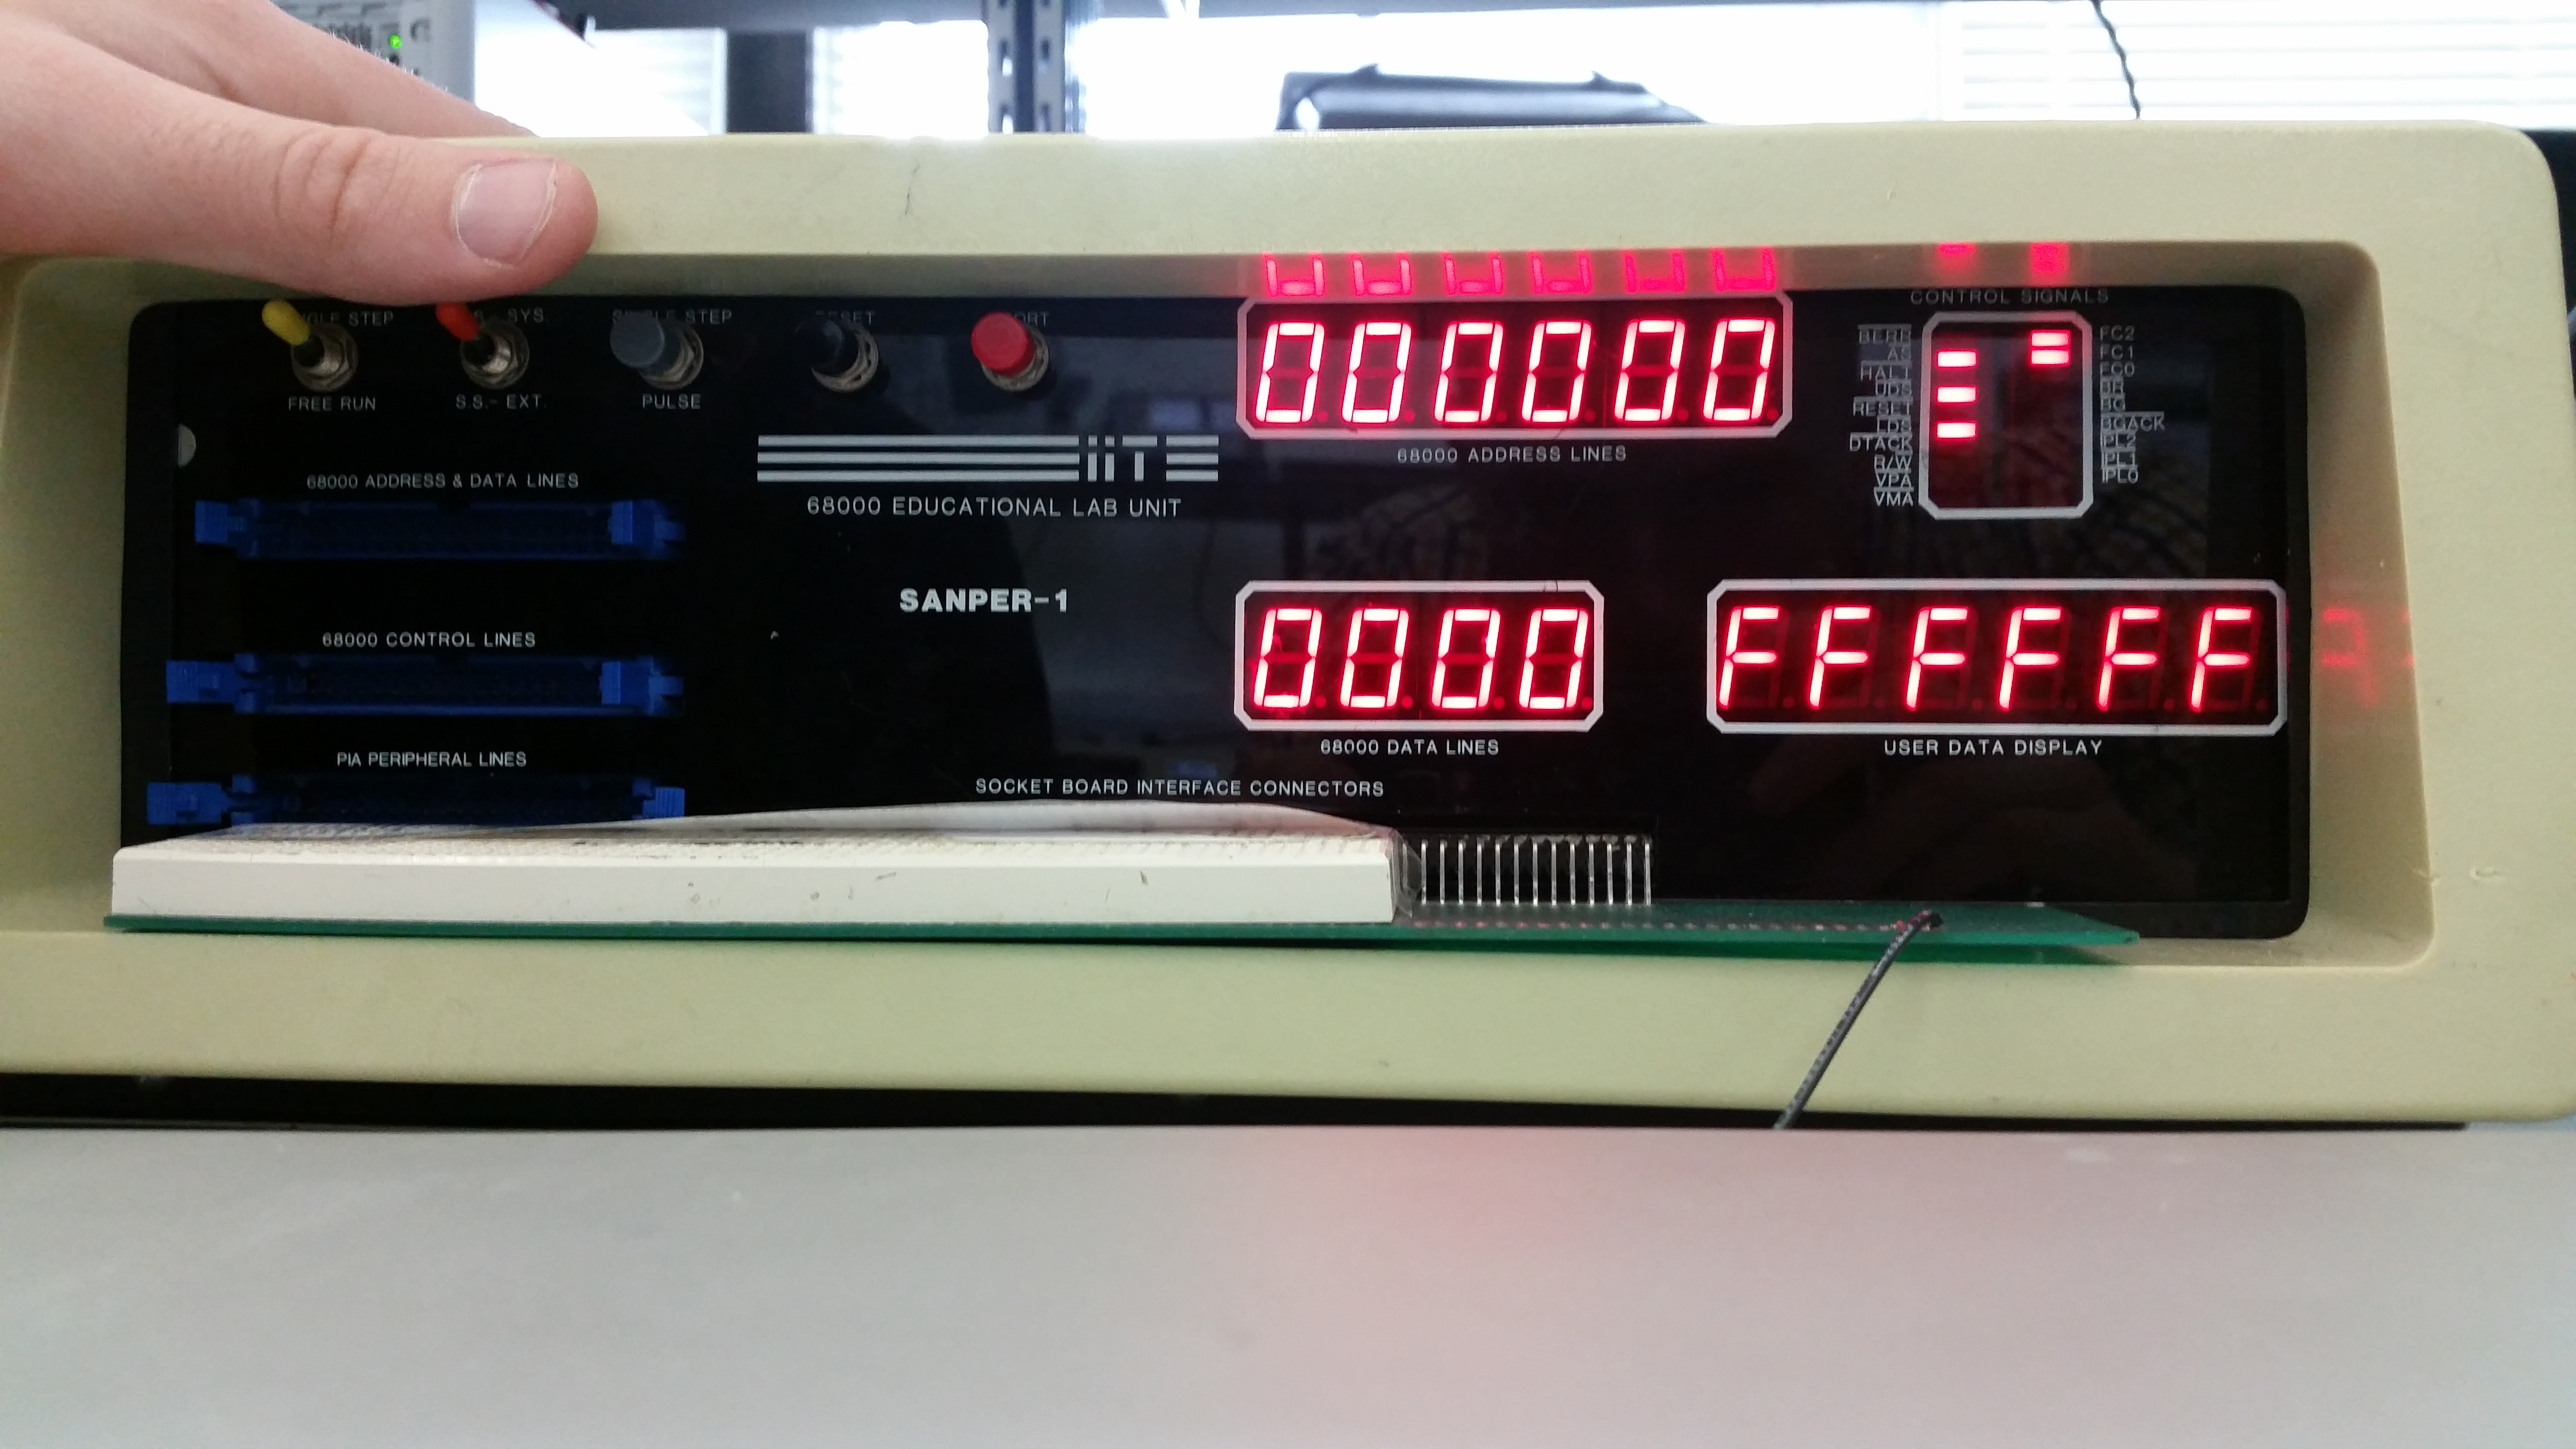
\includegraphics[width=1\linewidth]{Lab1/20150120_094935}
\end{center}
\begin{center}
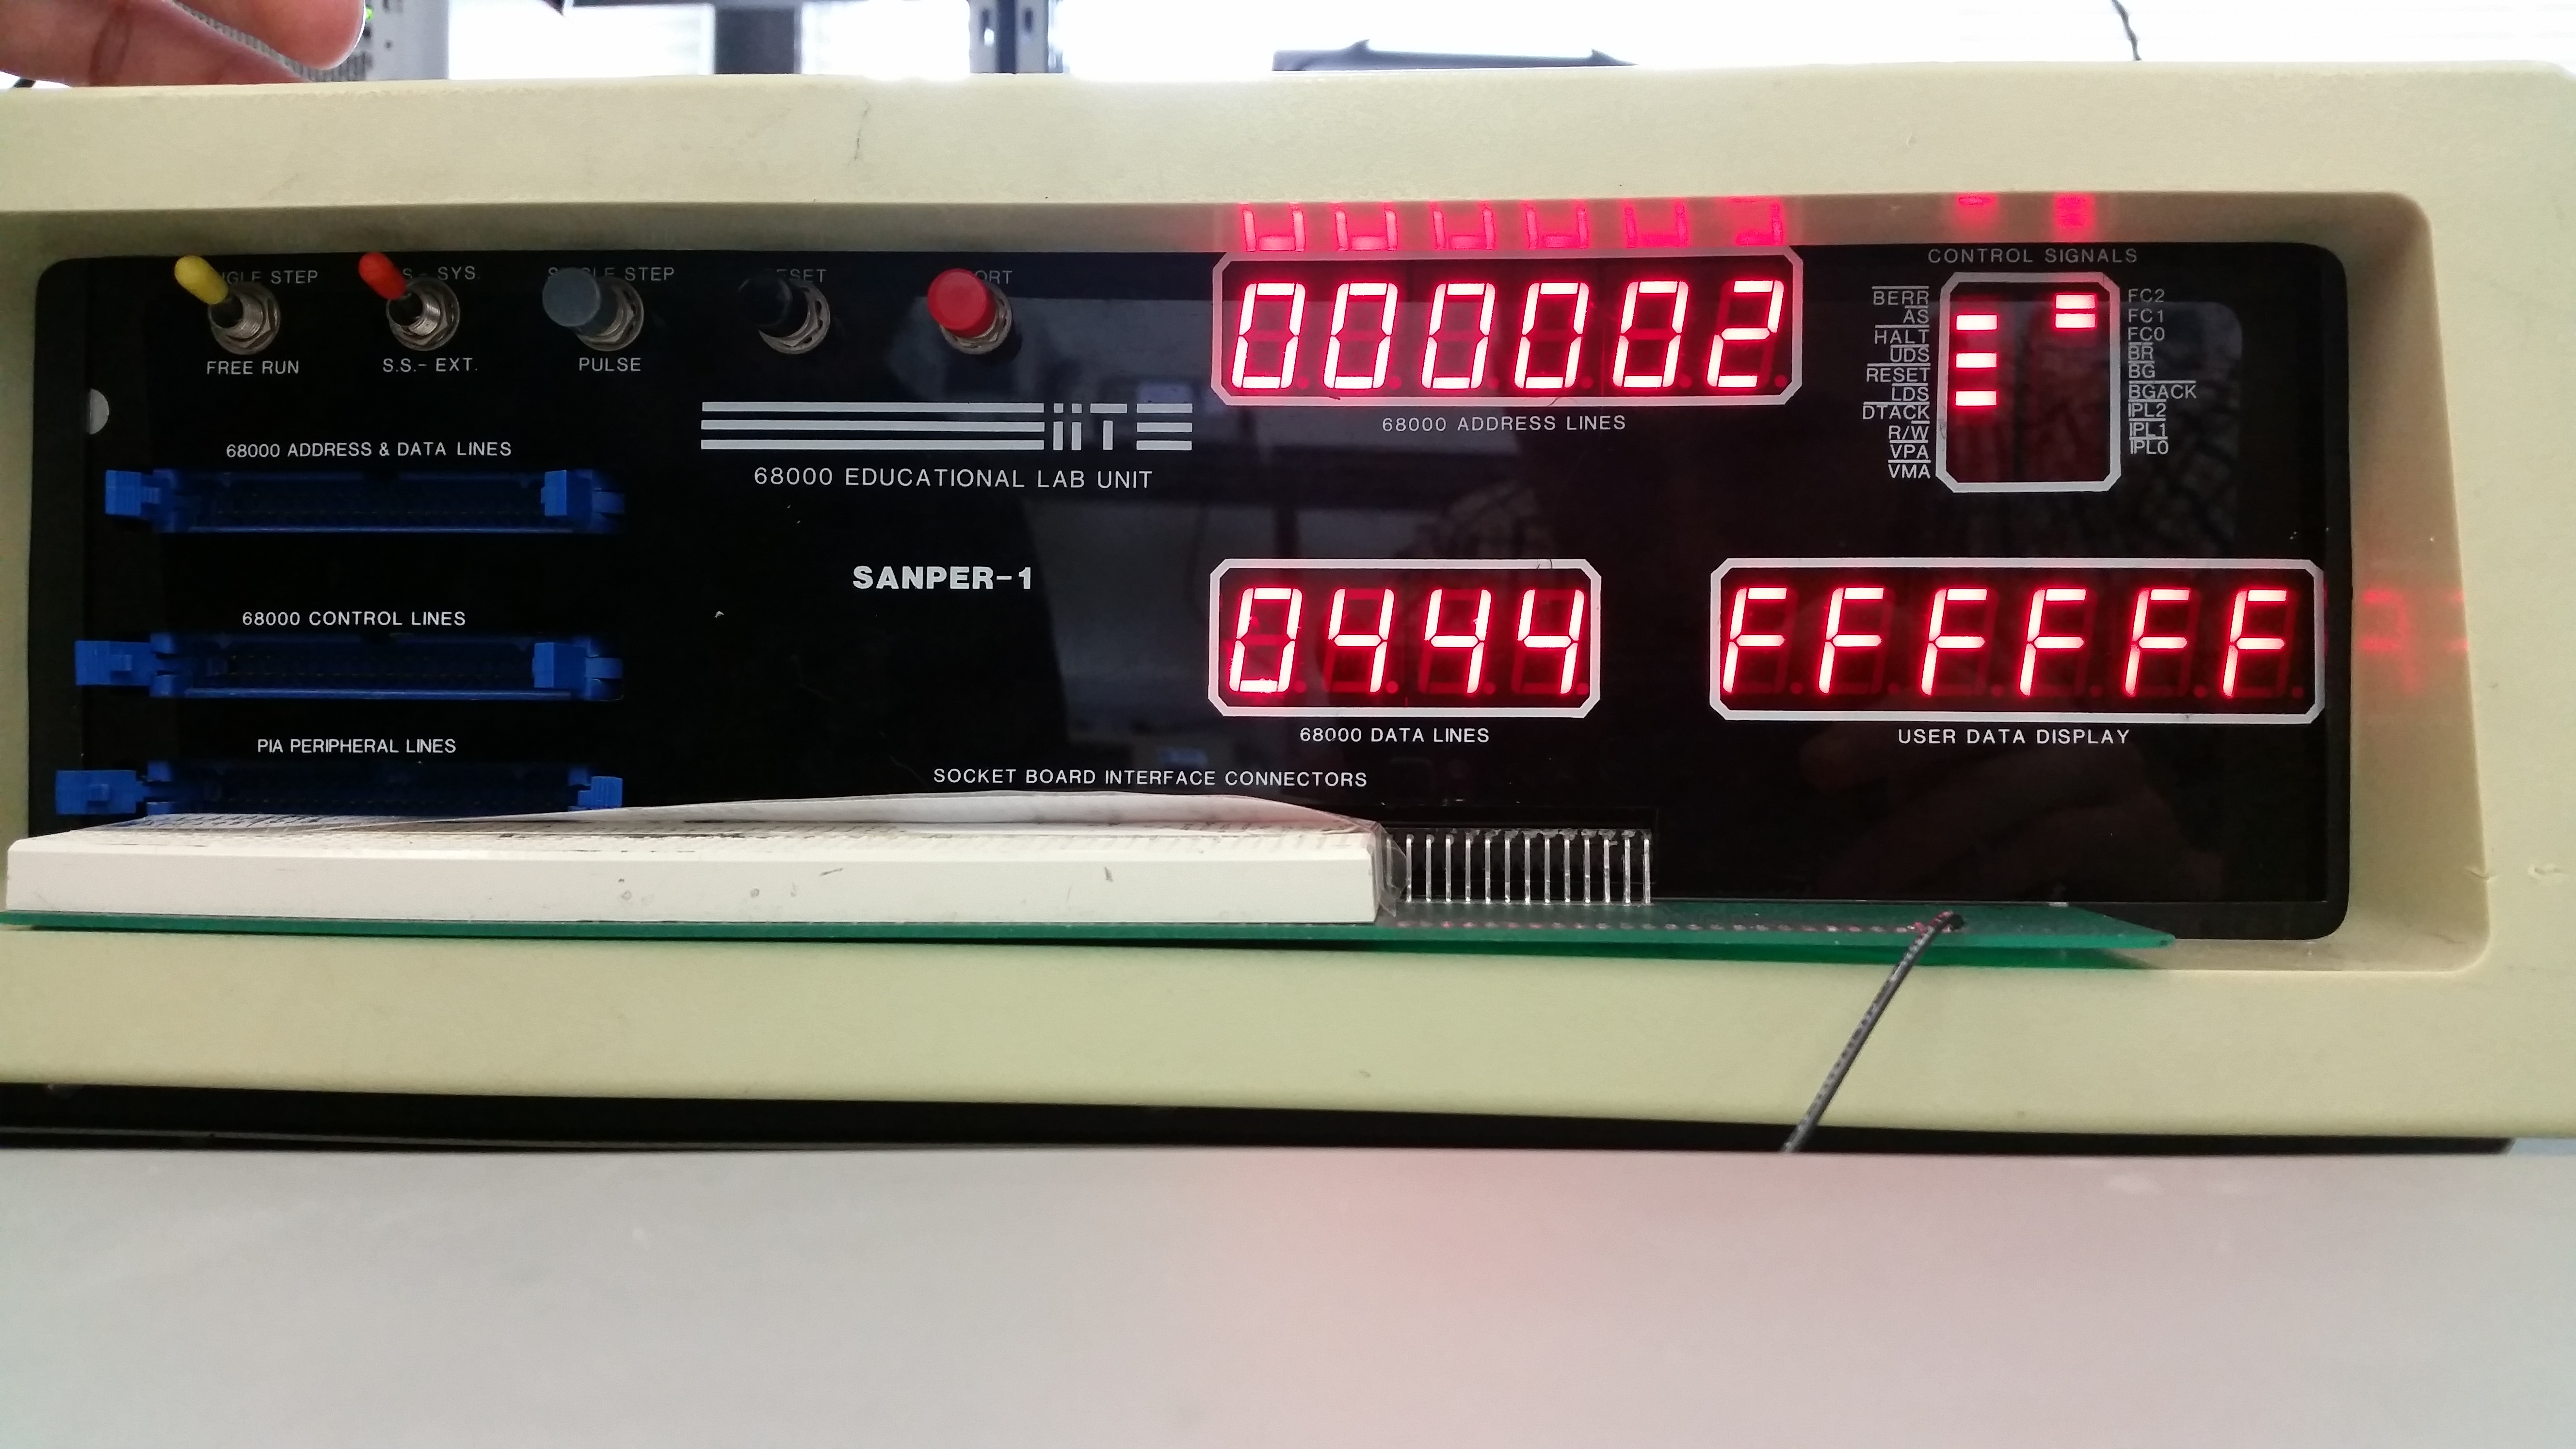
\includegraphics[width=1\linewidth]{Lab1/20150120_094945}
\end{center}
\begin{center}
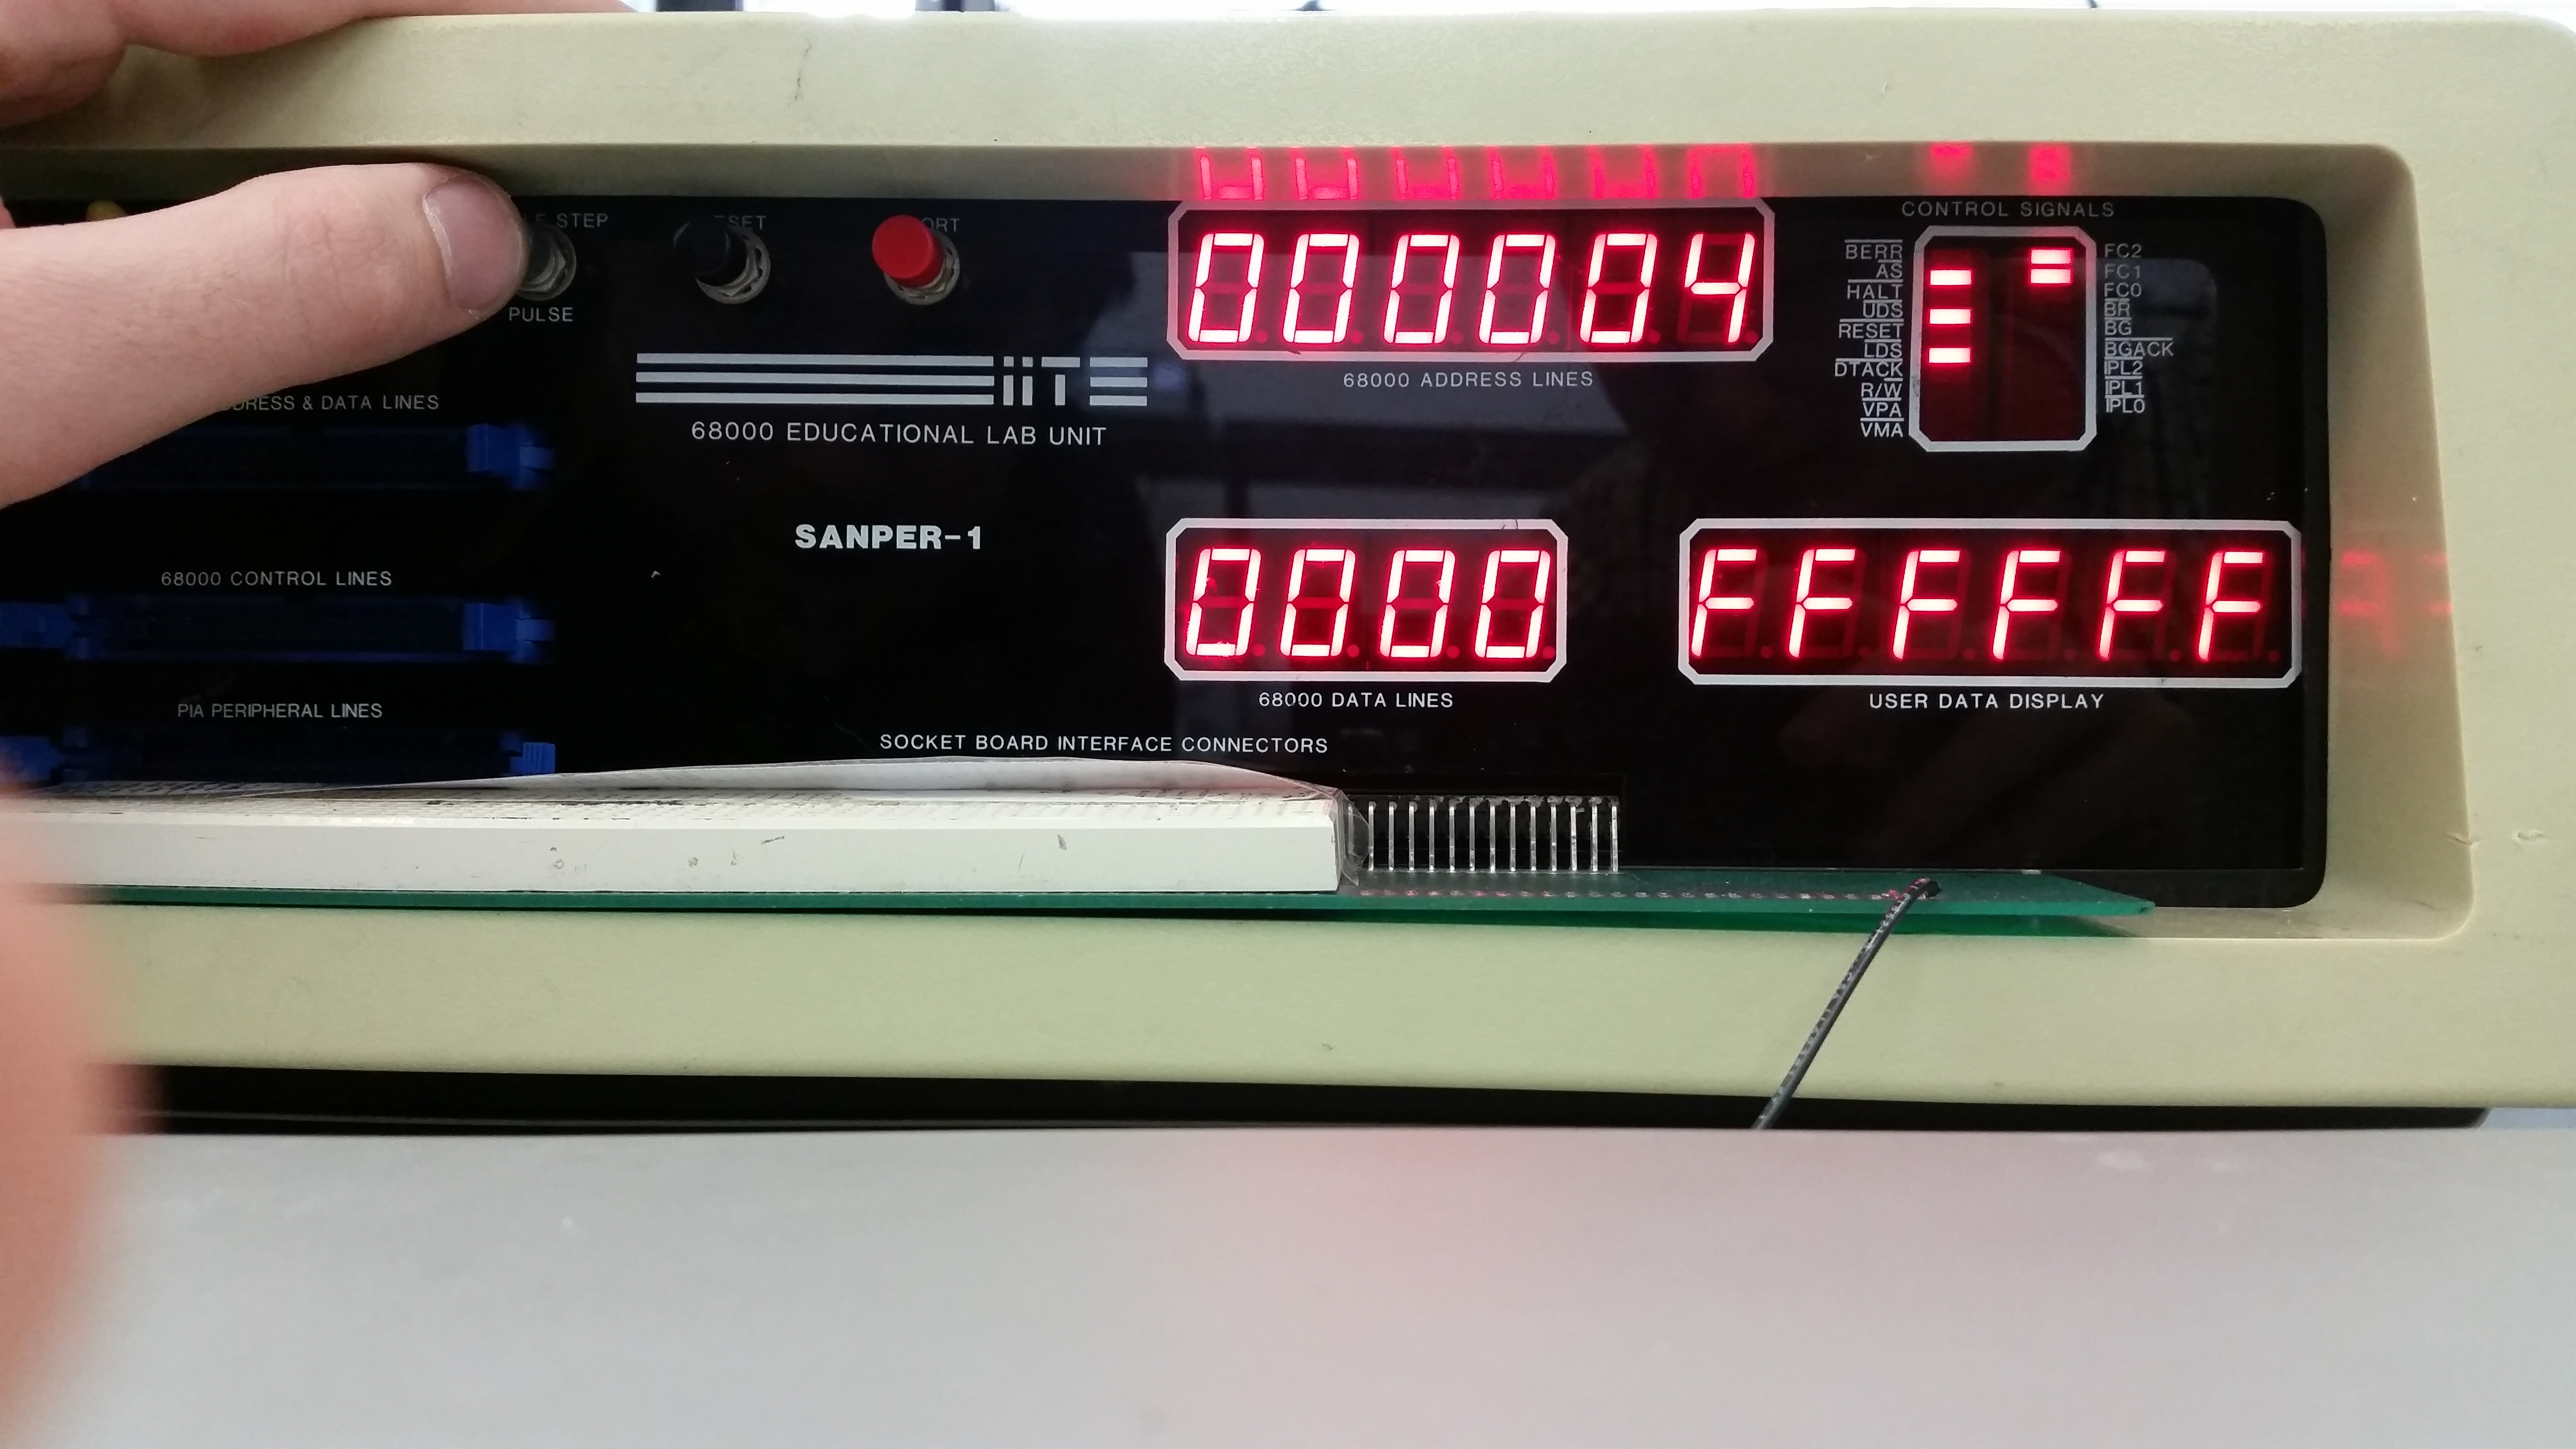
\includegraphics[width=1\linewidth]{Lab1/20150120_095003}
\end{center}
\begin{center}
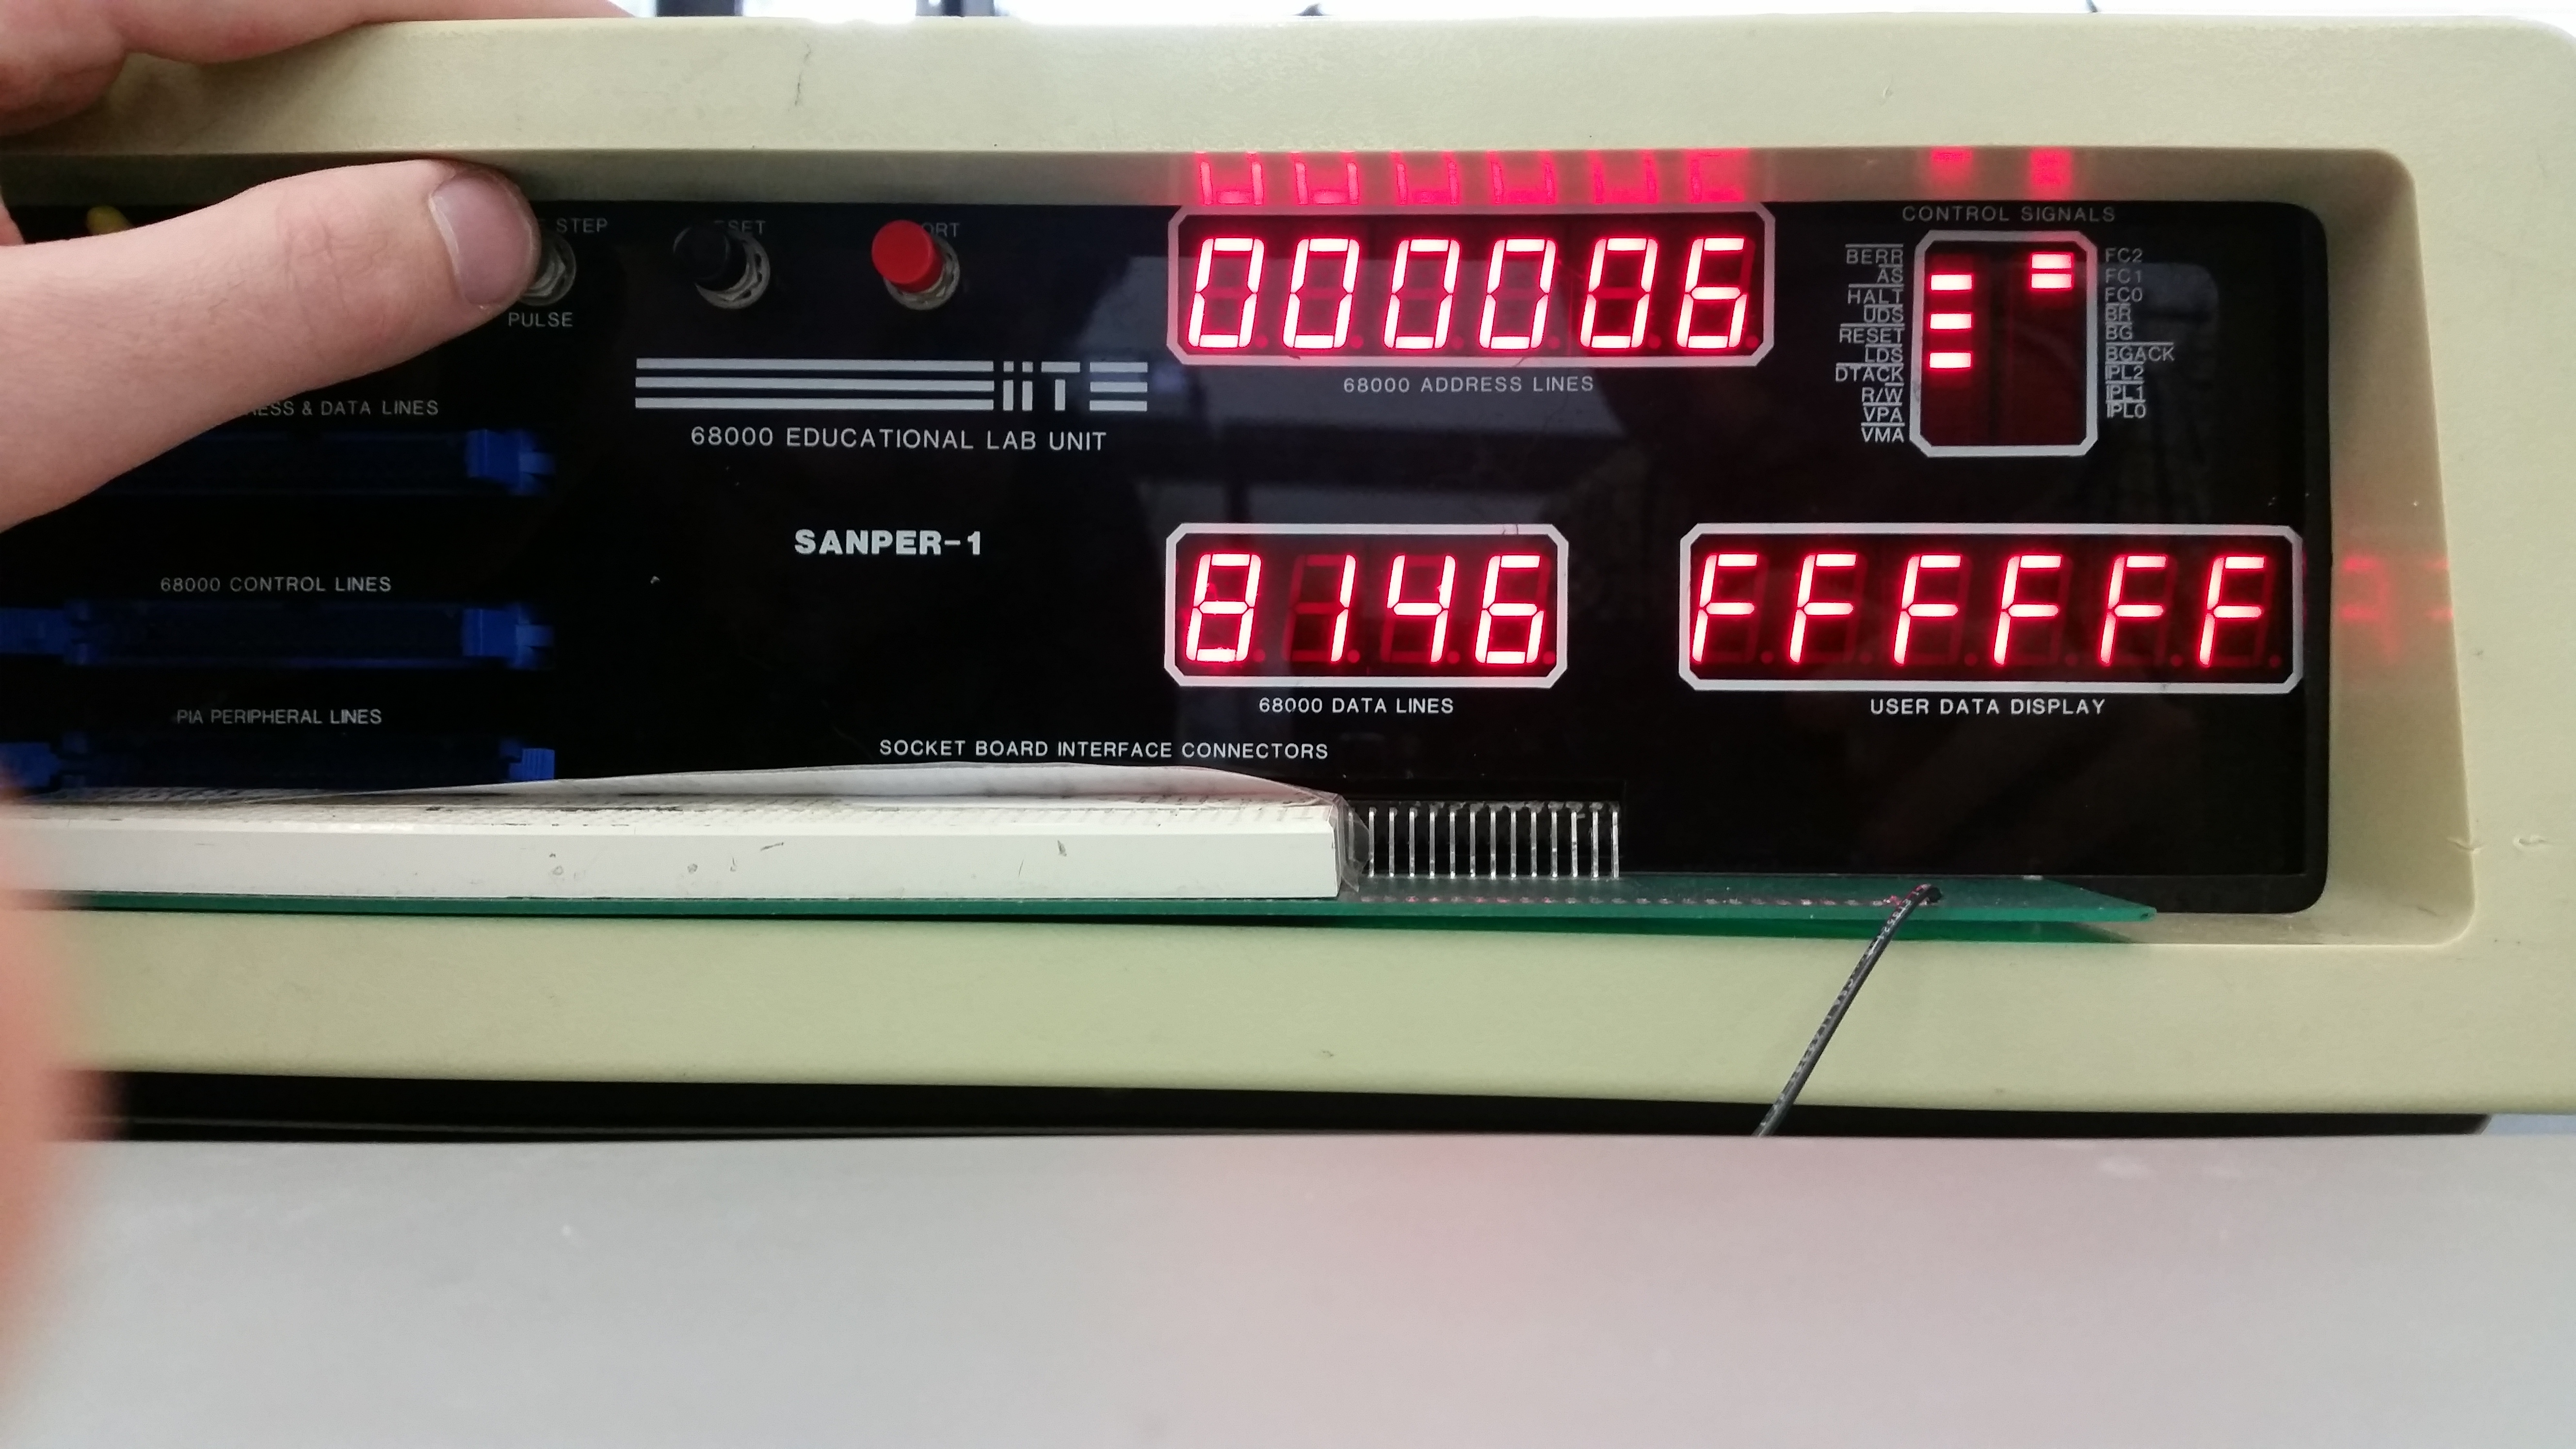
\includegraphics[width=1\linewidth]{Lab1/20150120_095005}
\end{center}
\begin{center}
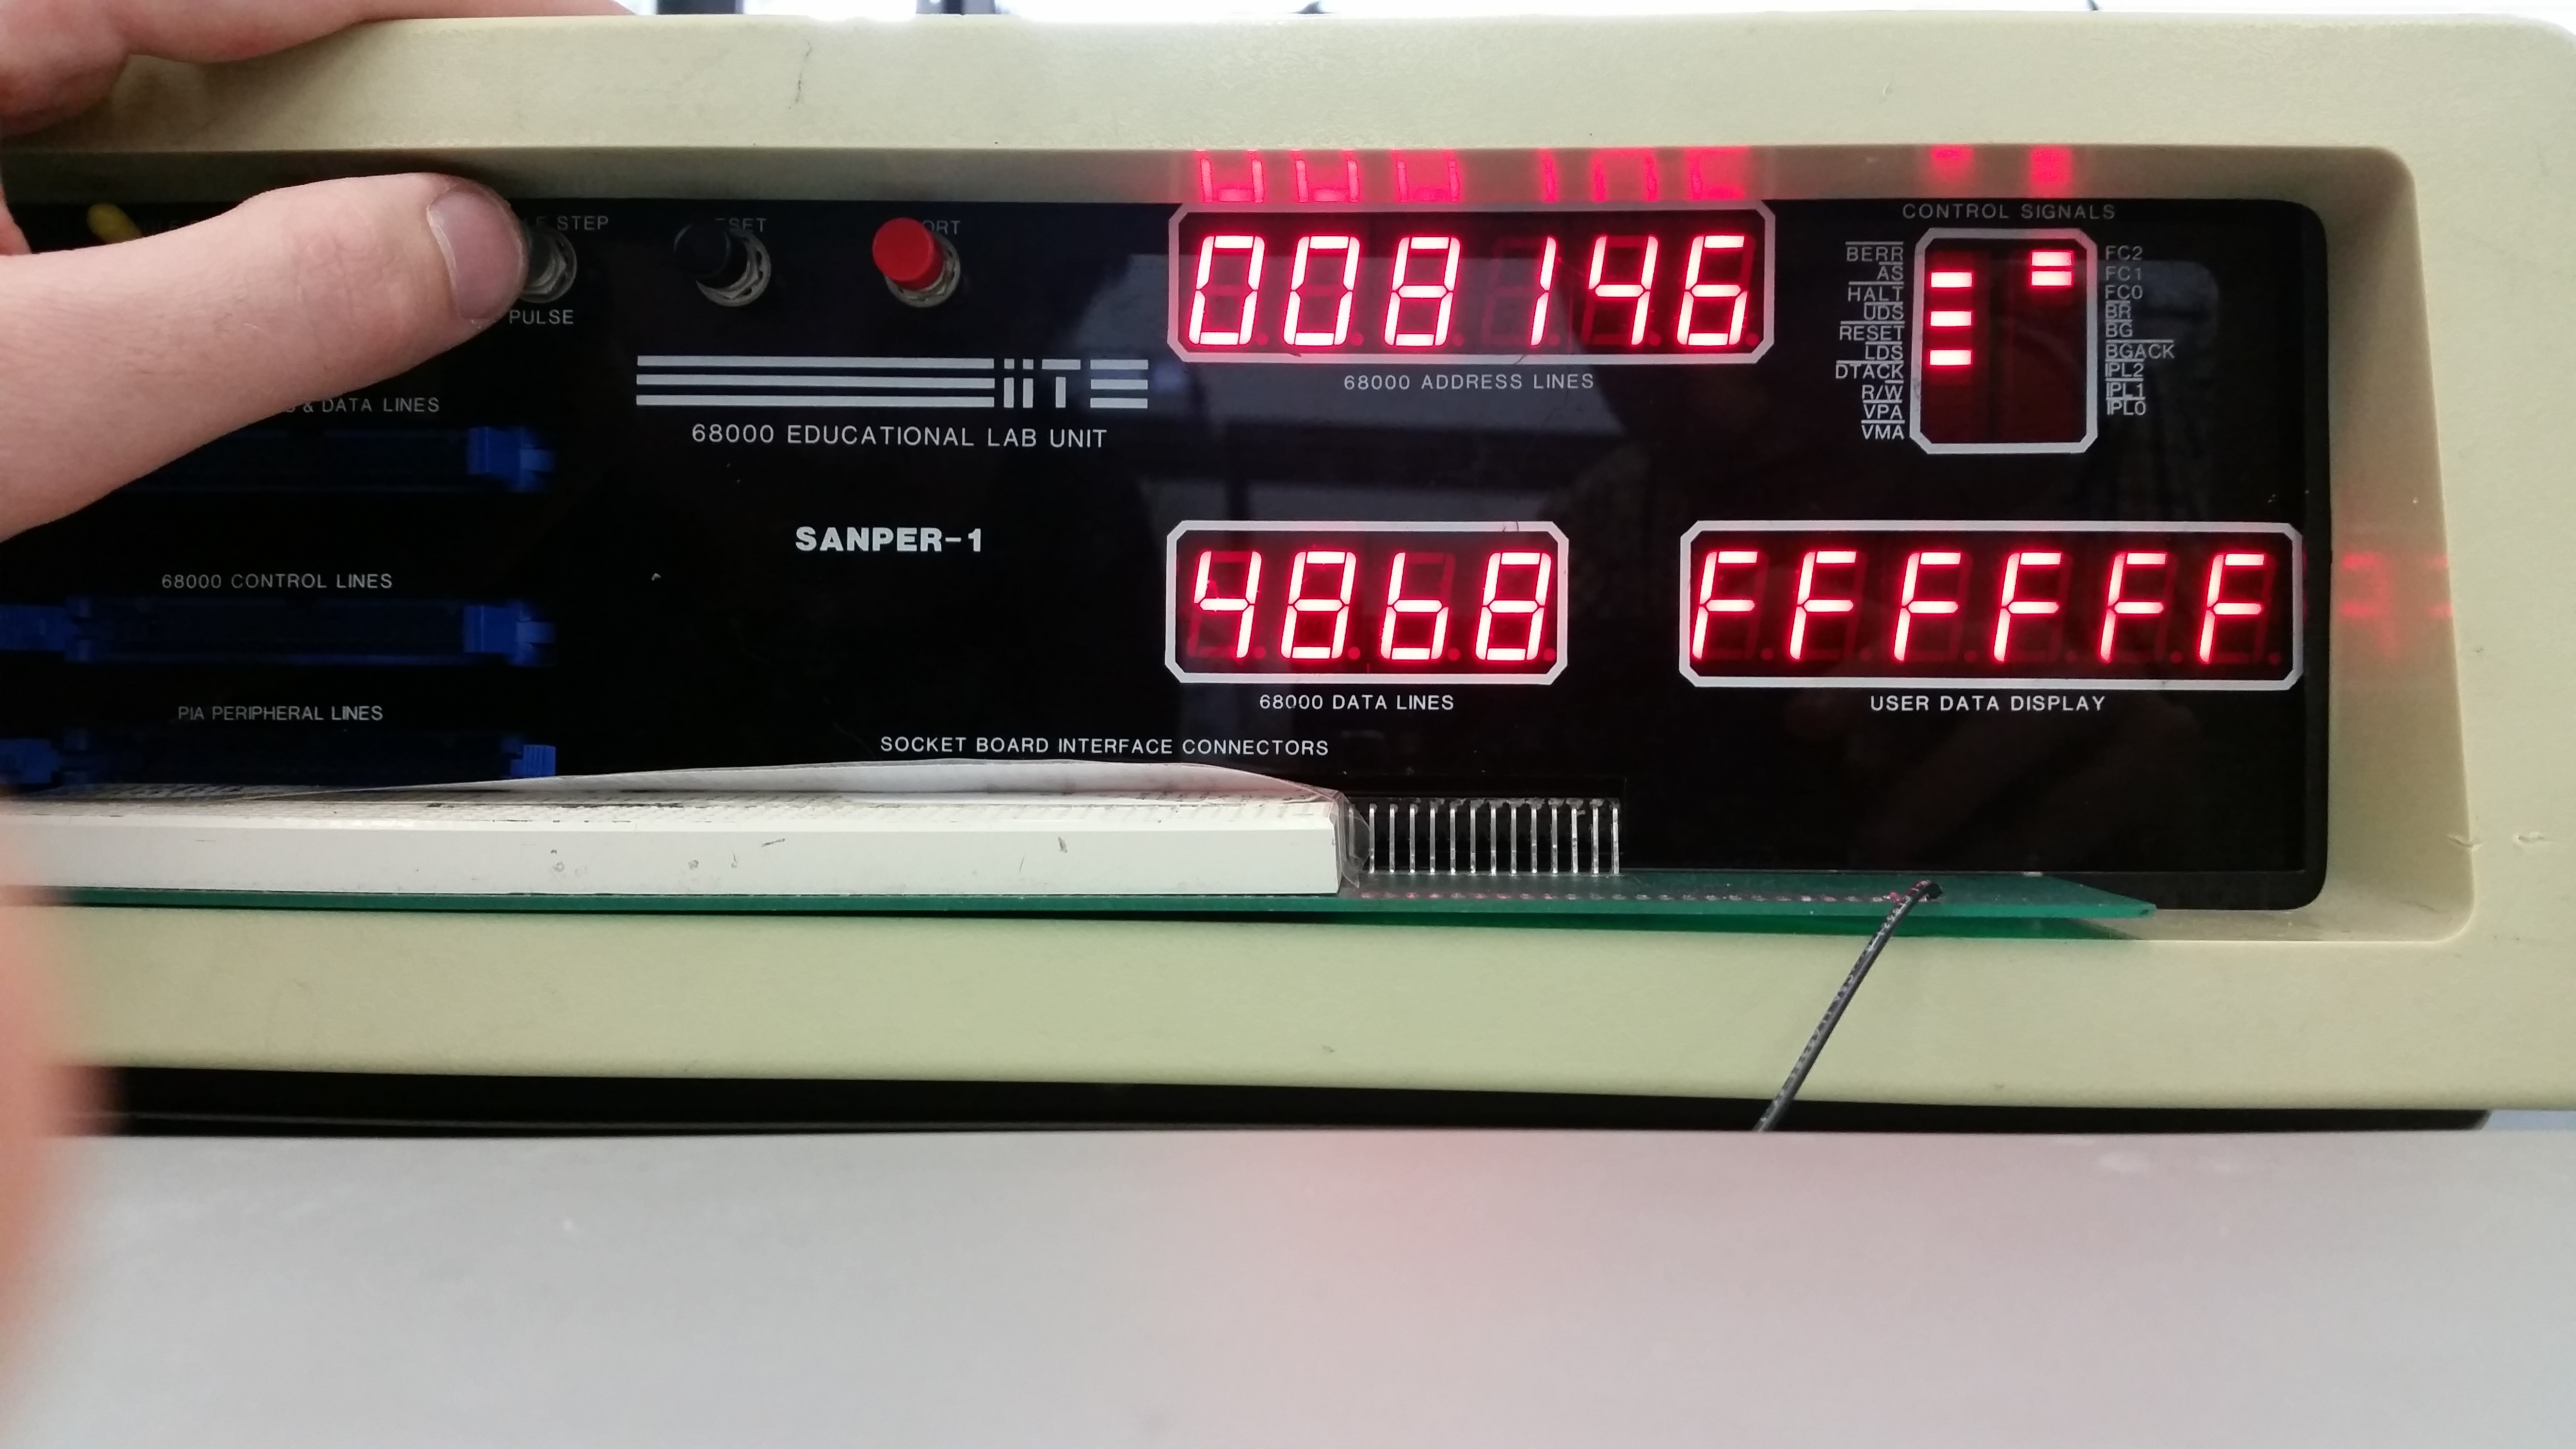
\includegraphics[width=1\linewidth]{Lab1/20150120_095007}
\end{center}
\begin{center}
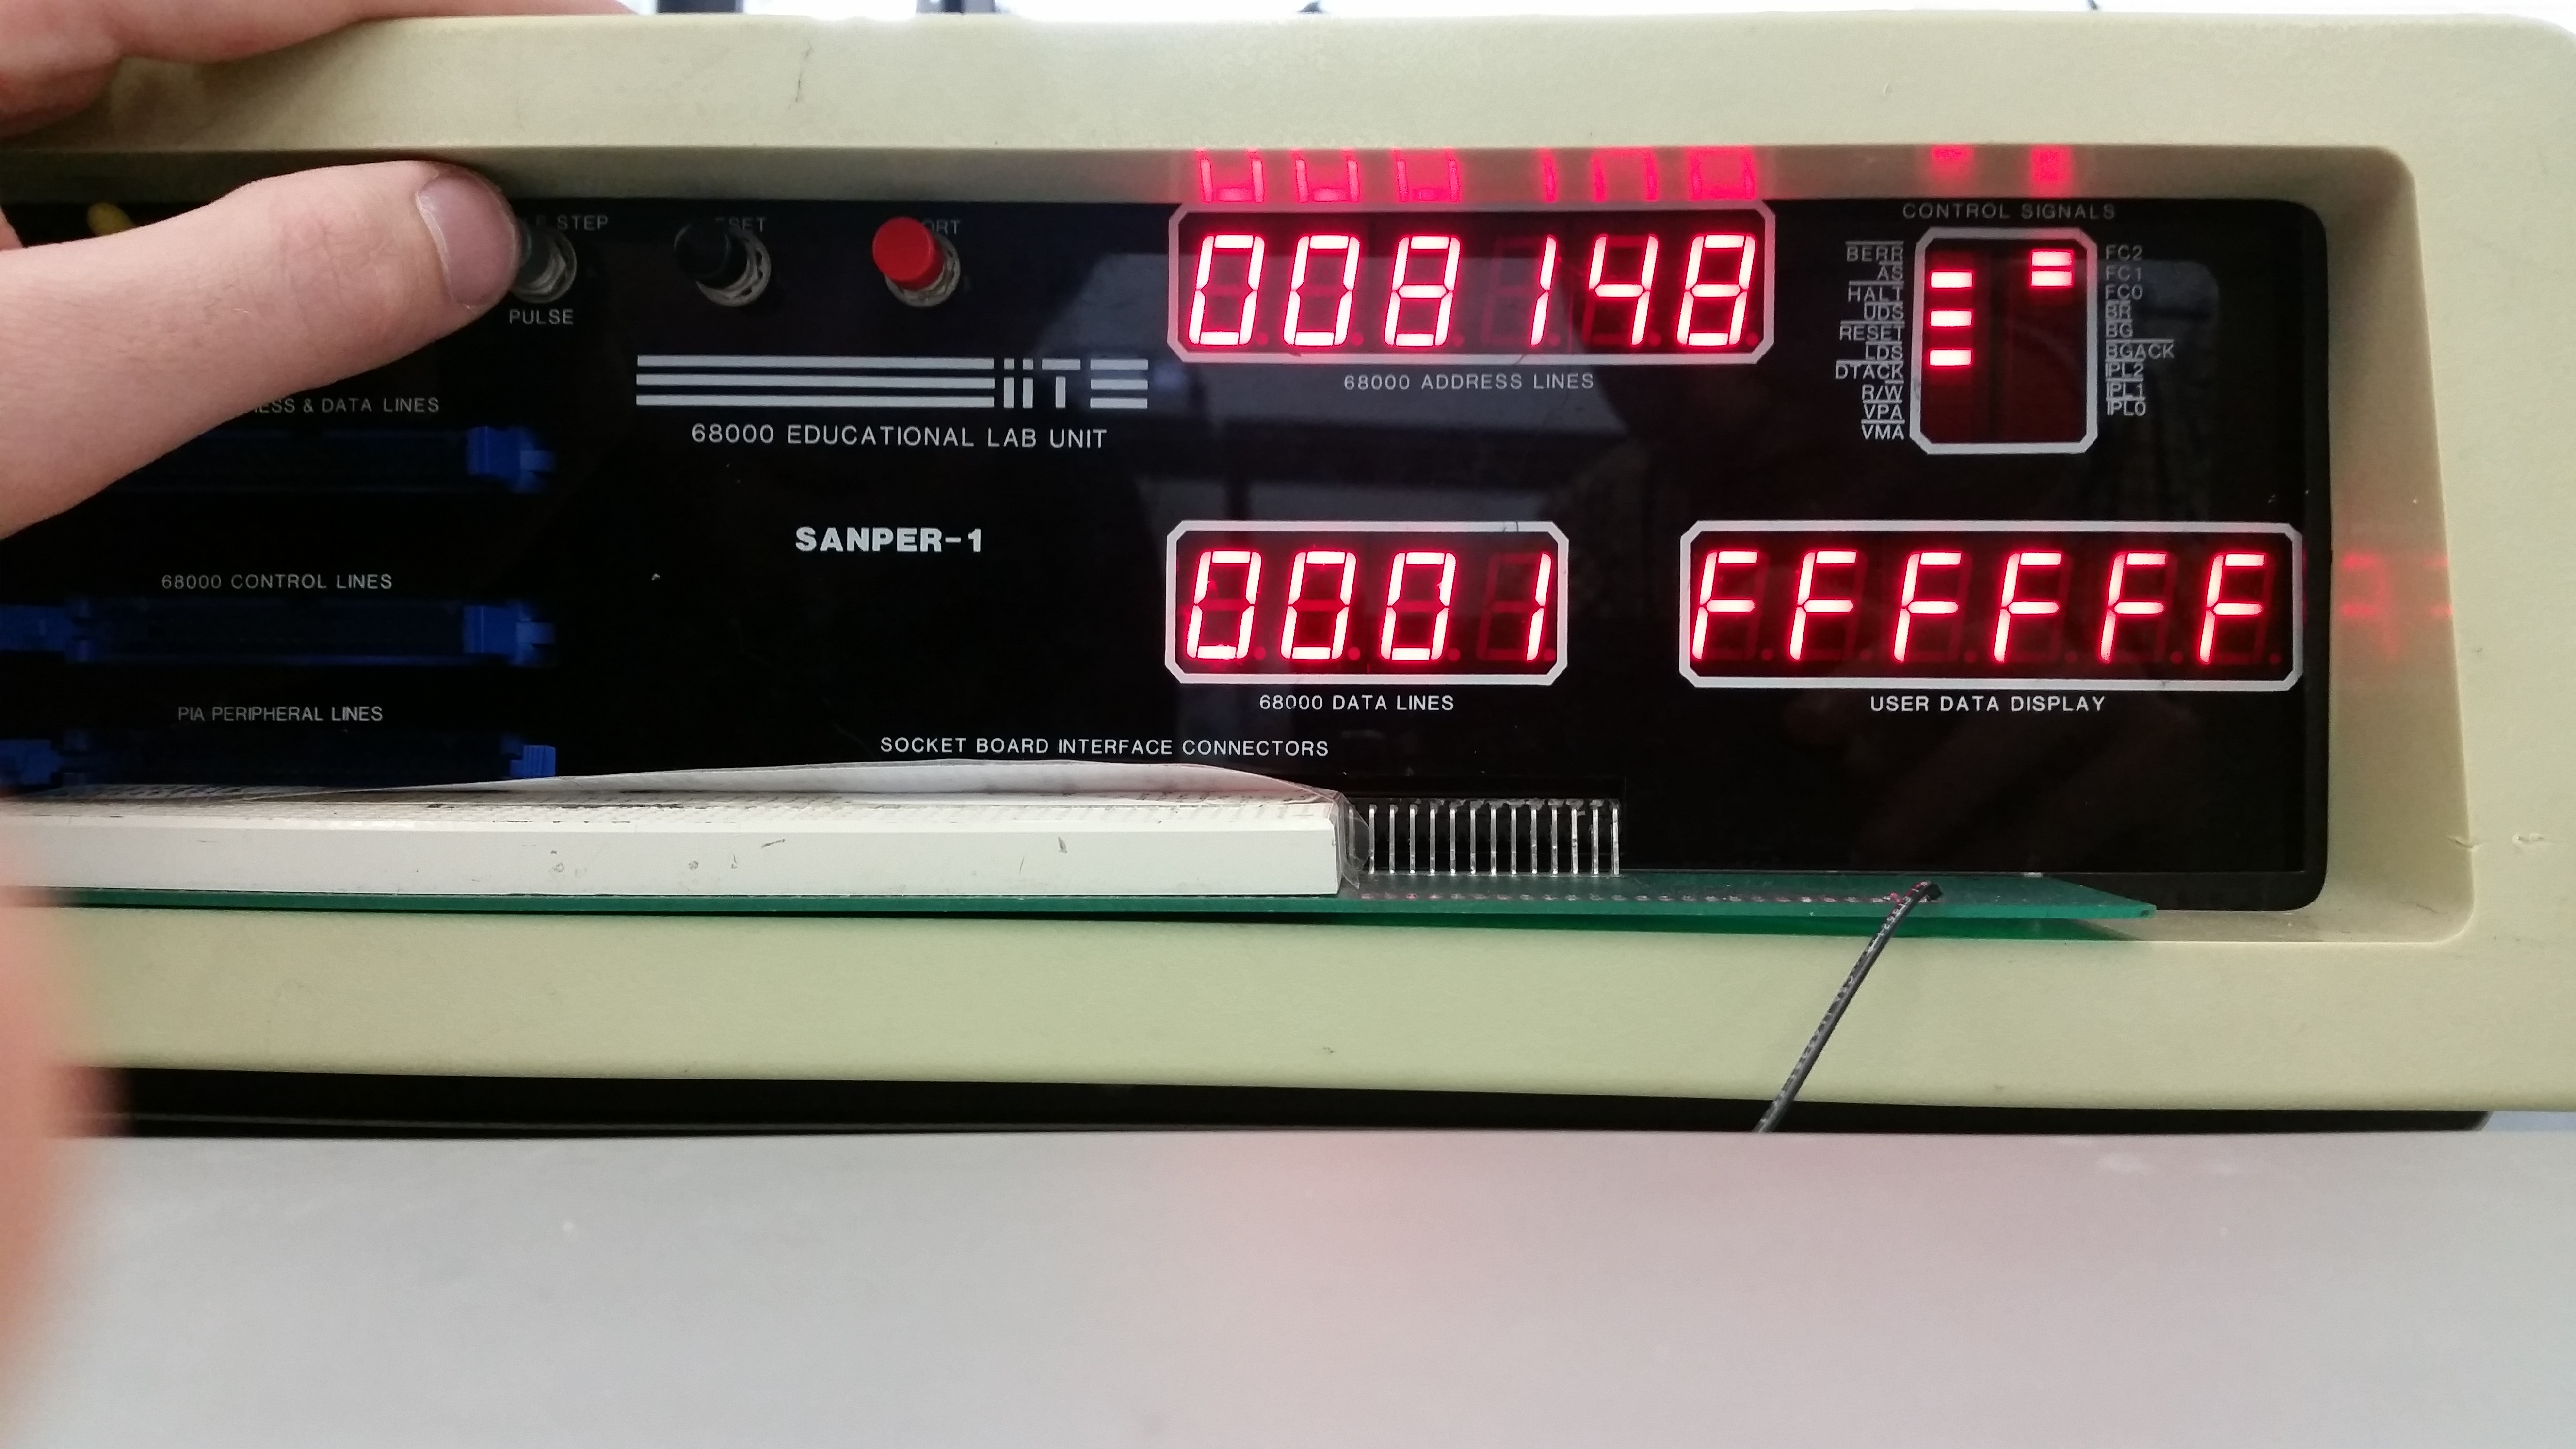
\includegraphics[width=1\linewidth]{Lab1/20150120_095009}
\end{center}
\begin{center}
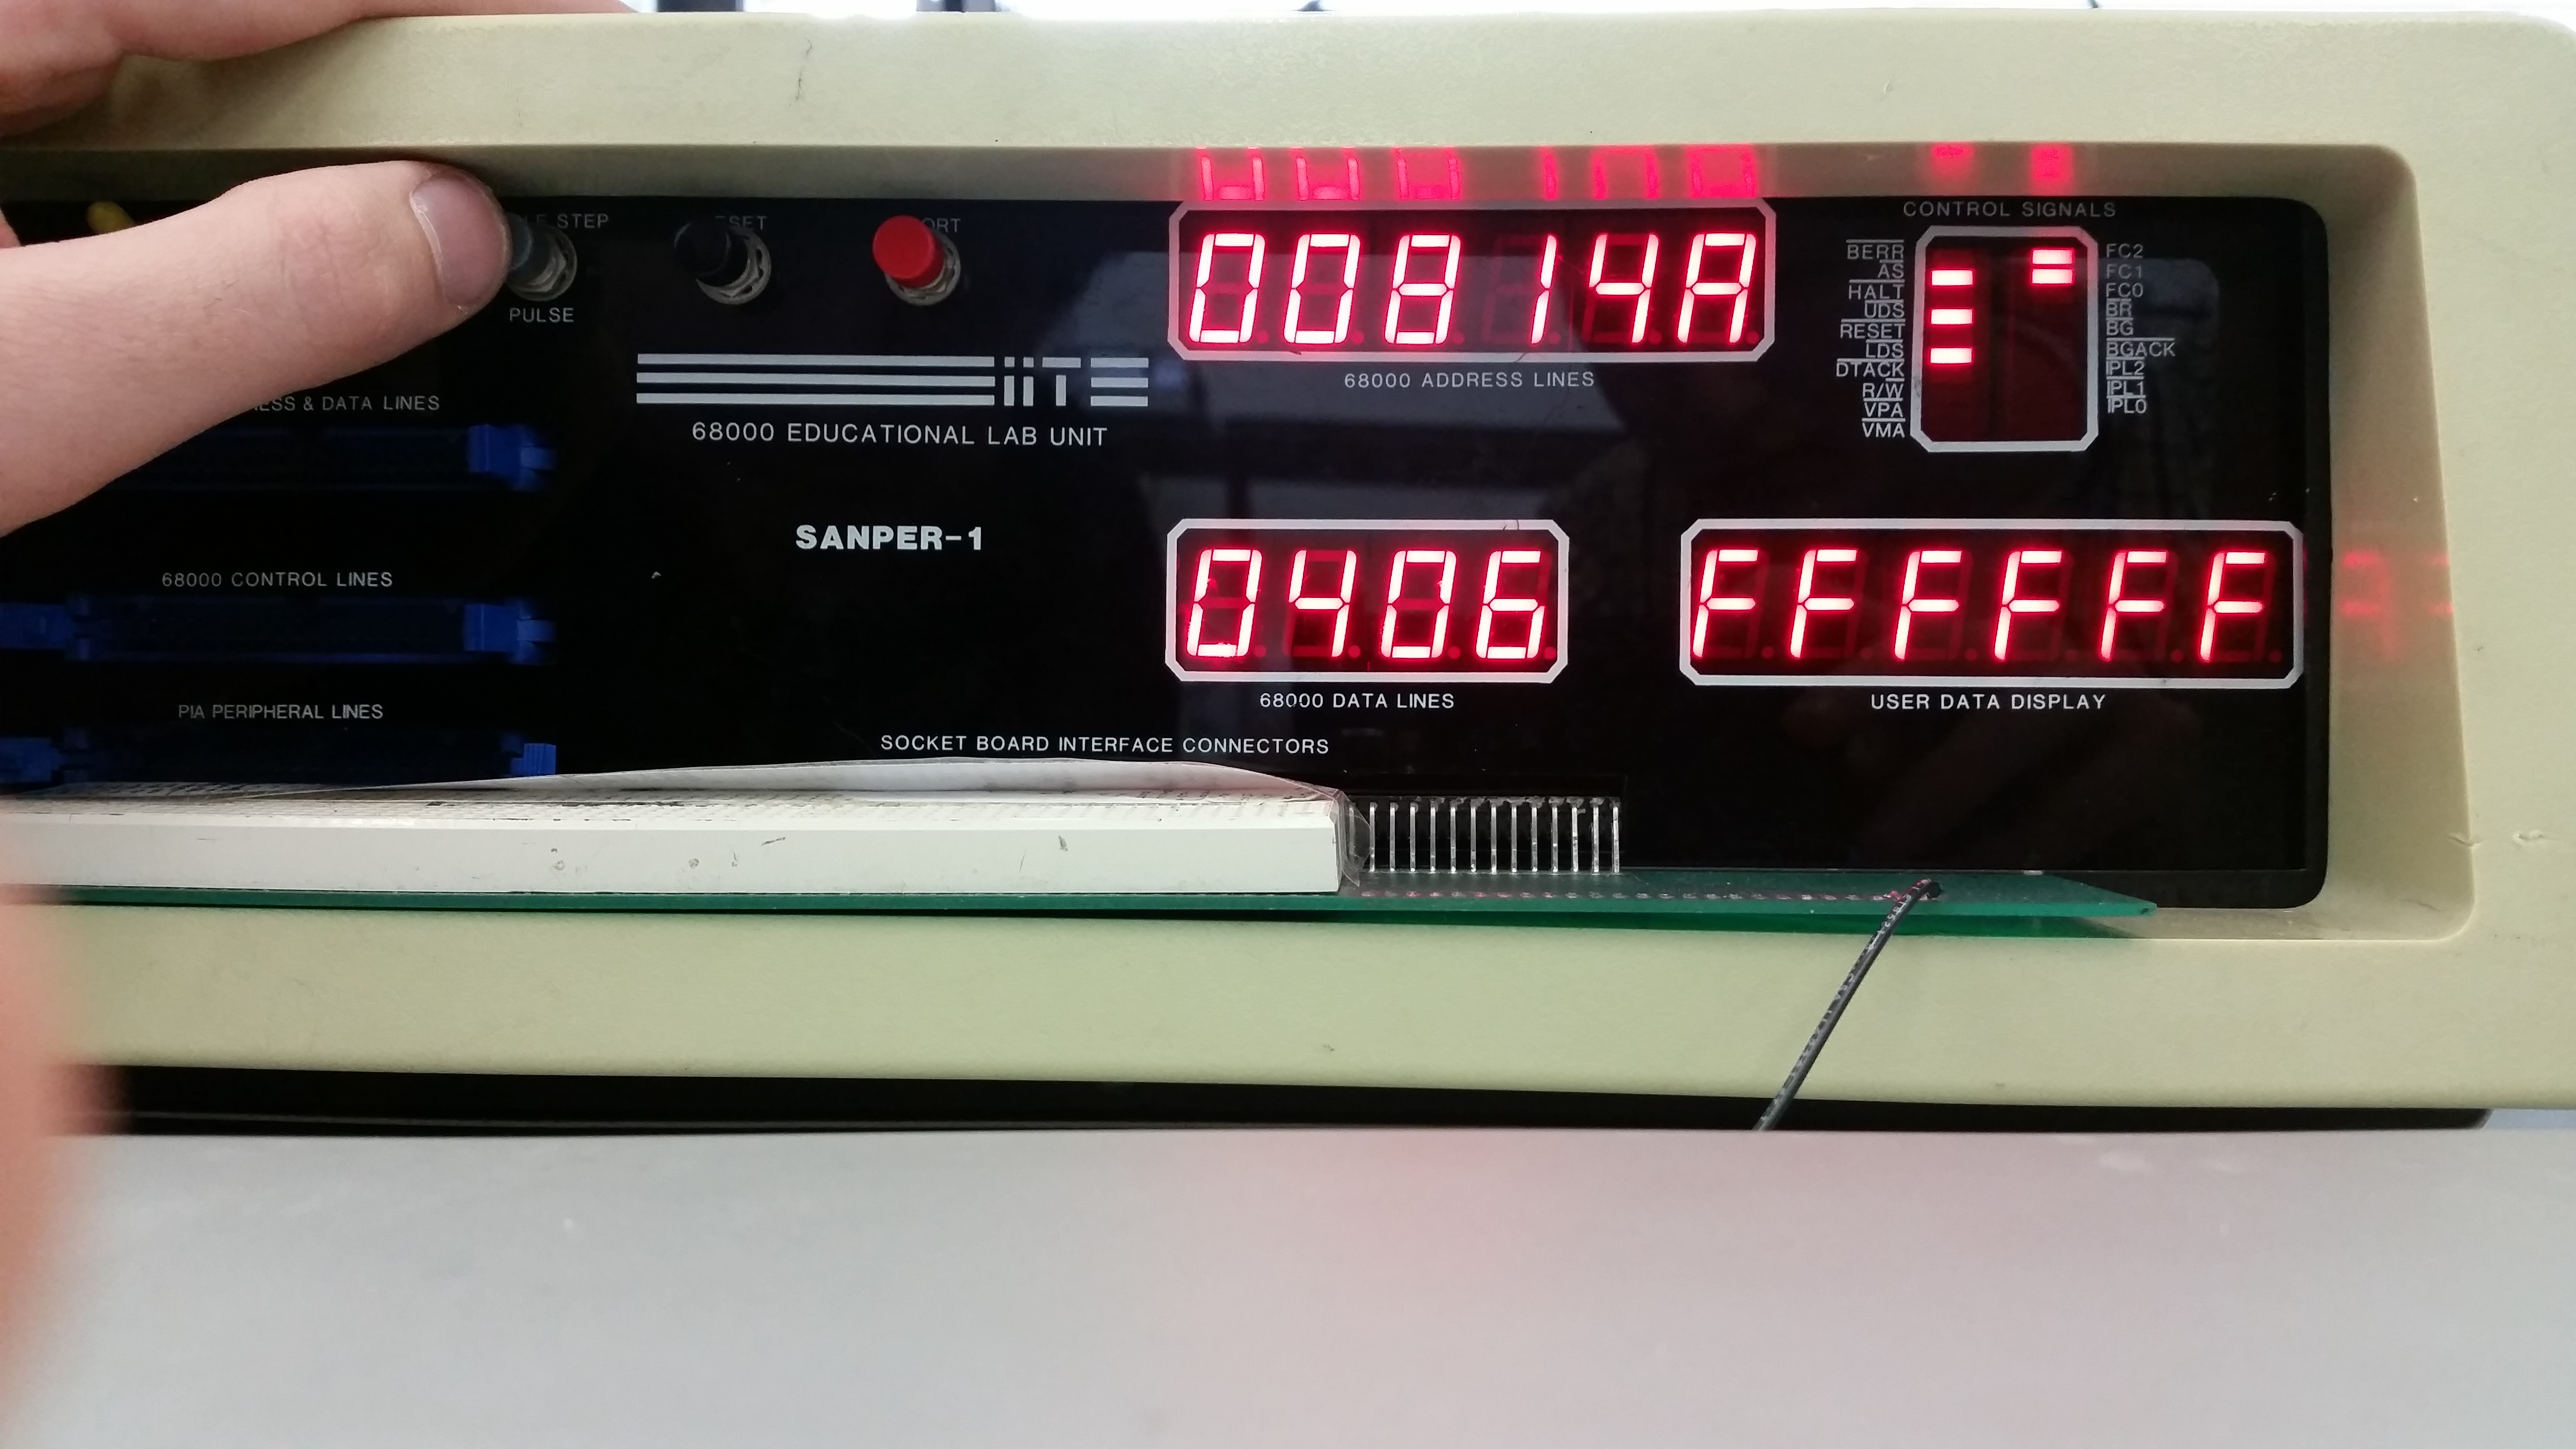
\includegraphics[width=1\linewidth]{Lab1/20150120_095011}
\end{center}
\begin{center}
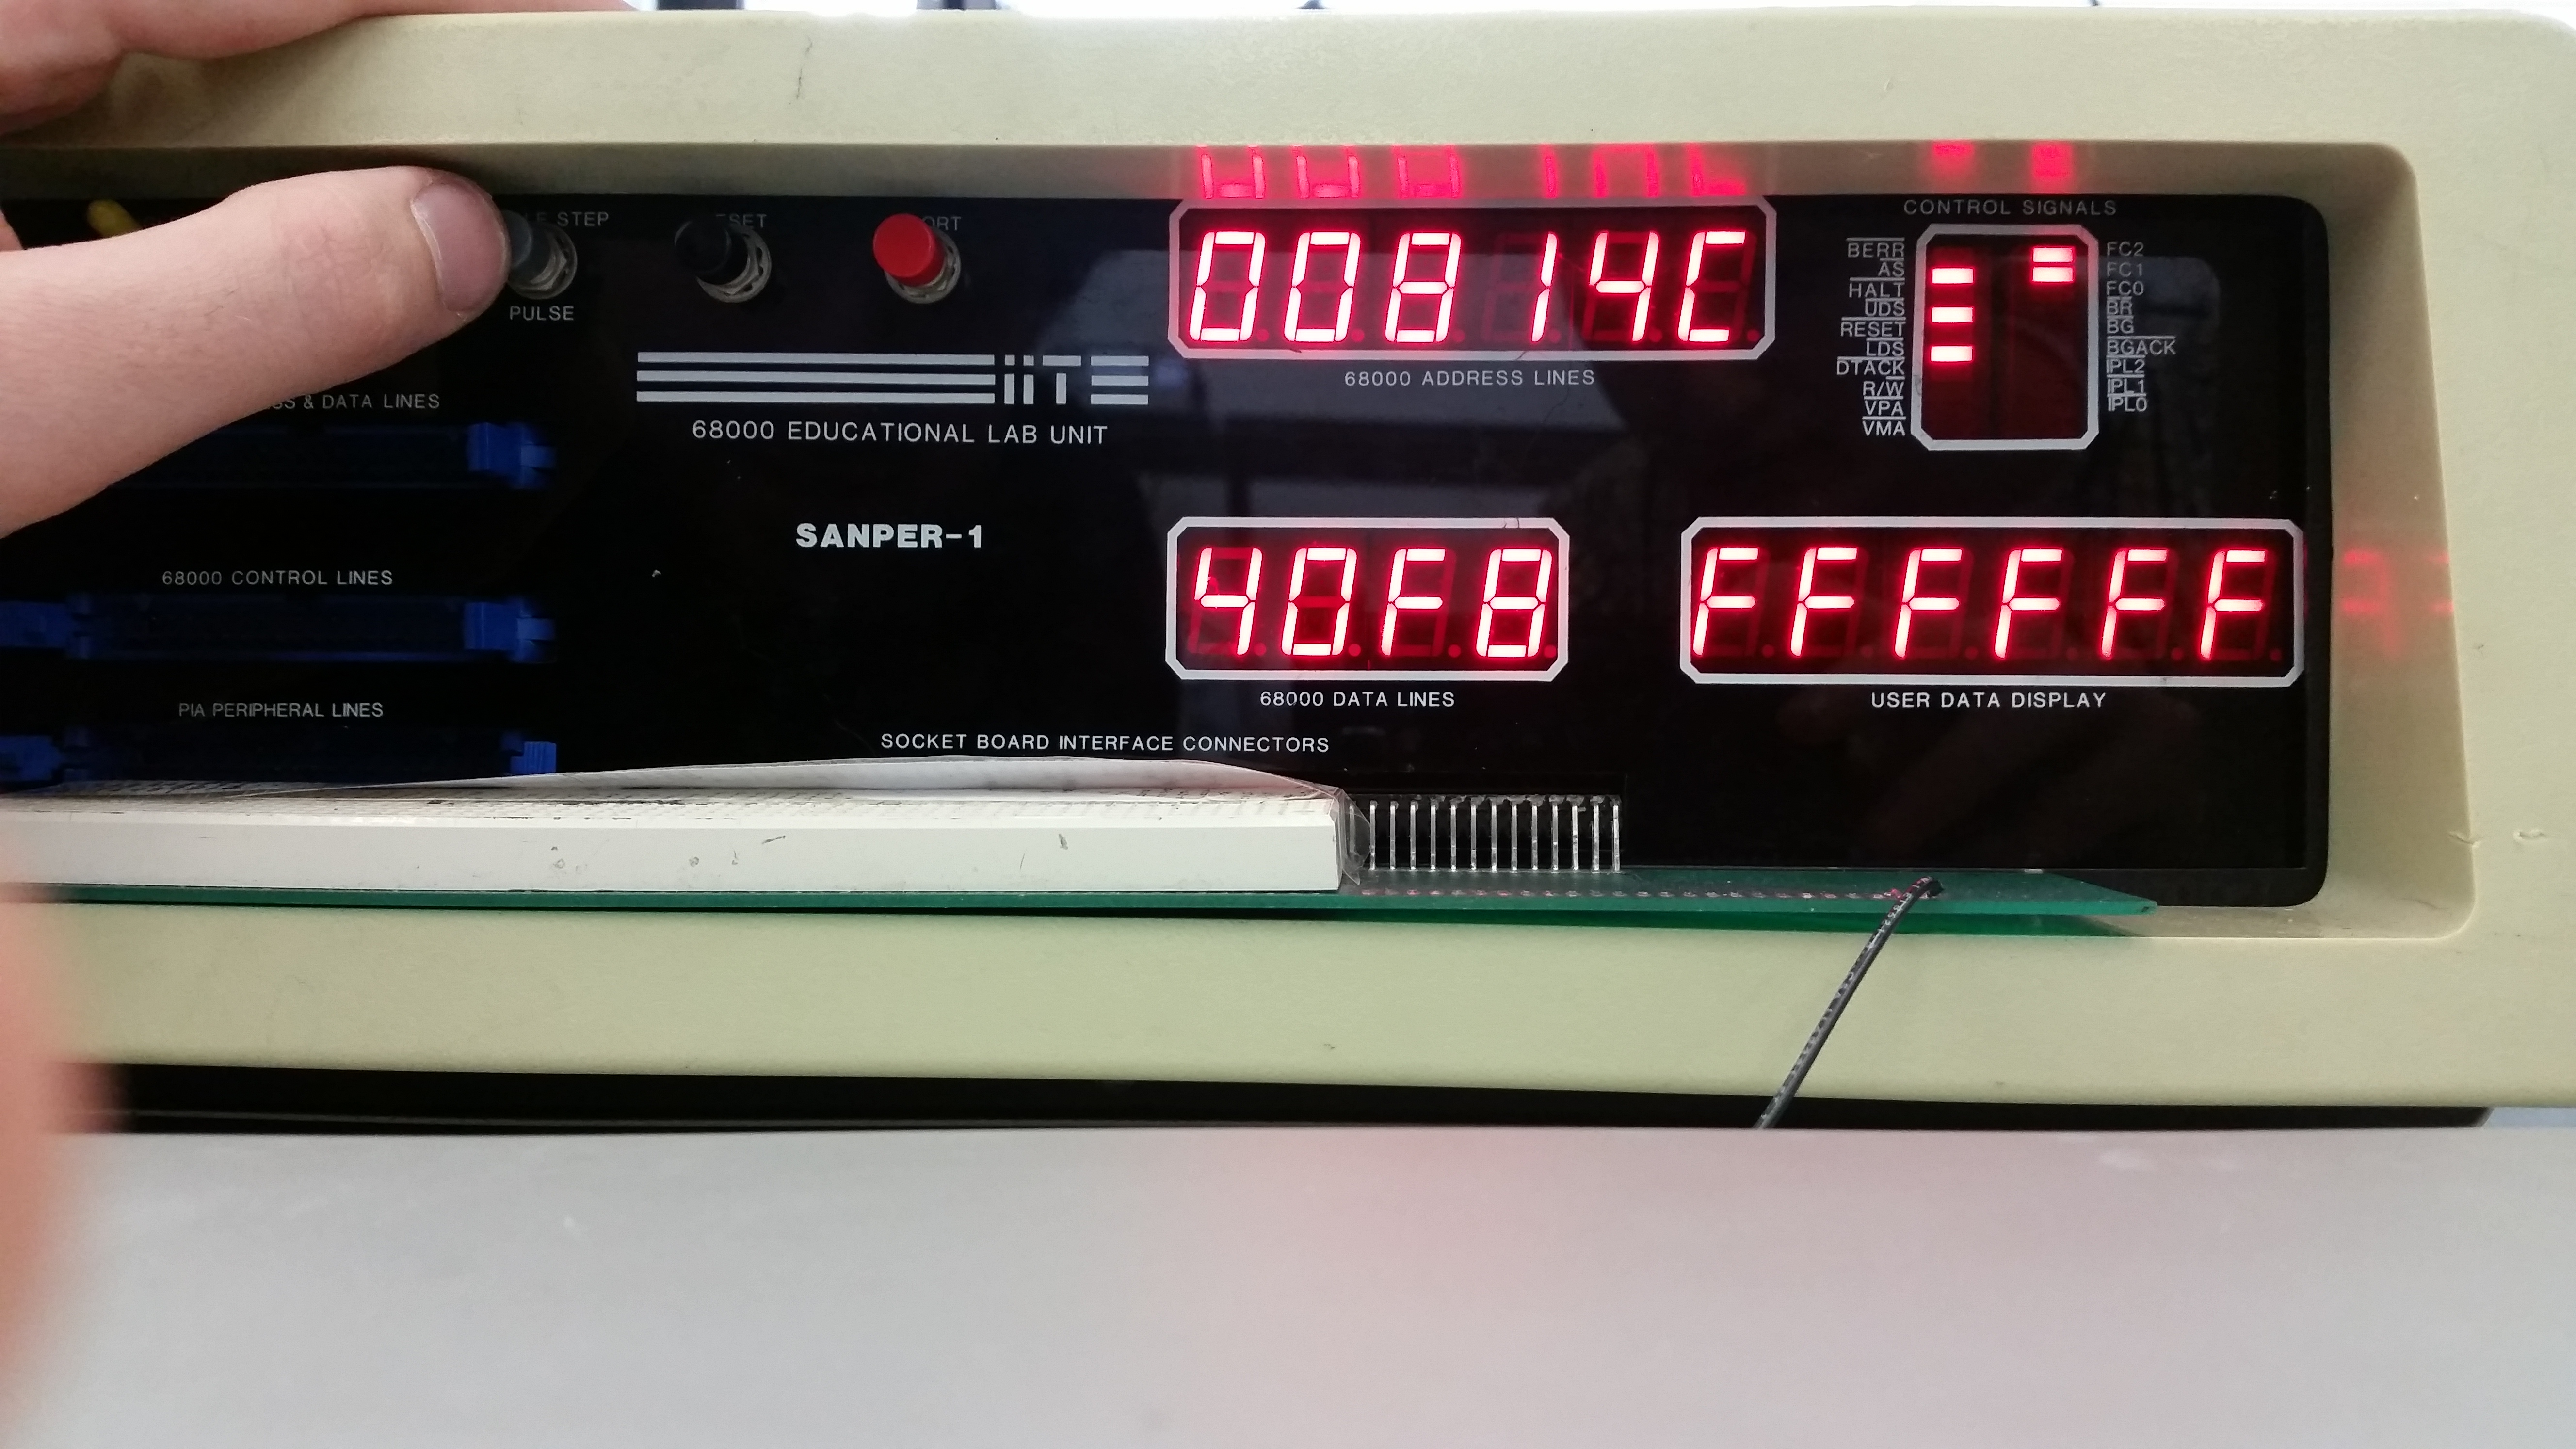
\includegraphics[width=1\linewidth]{Lab1/20150120_095012}
\end{center}
\begin{center}
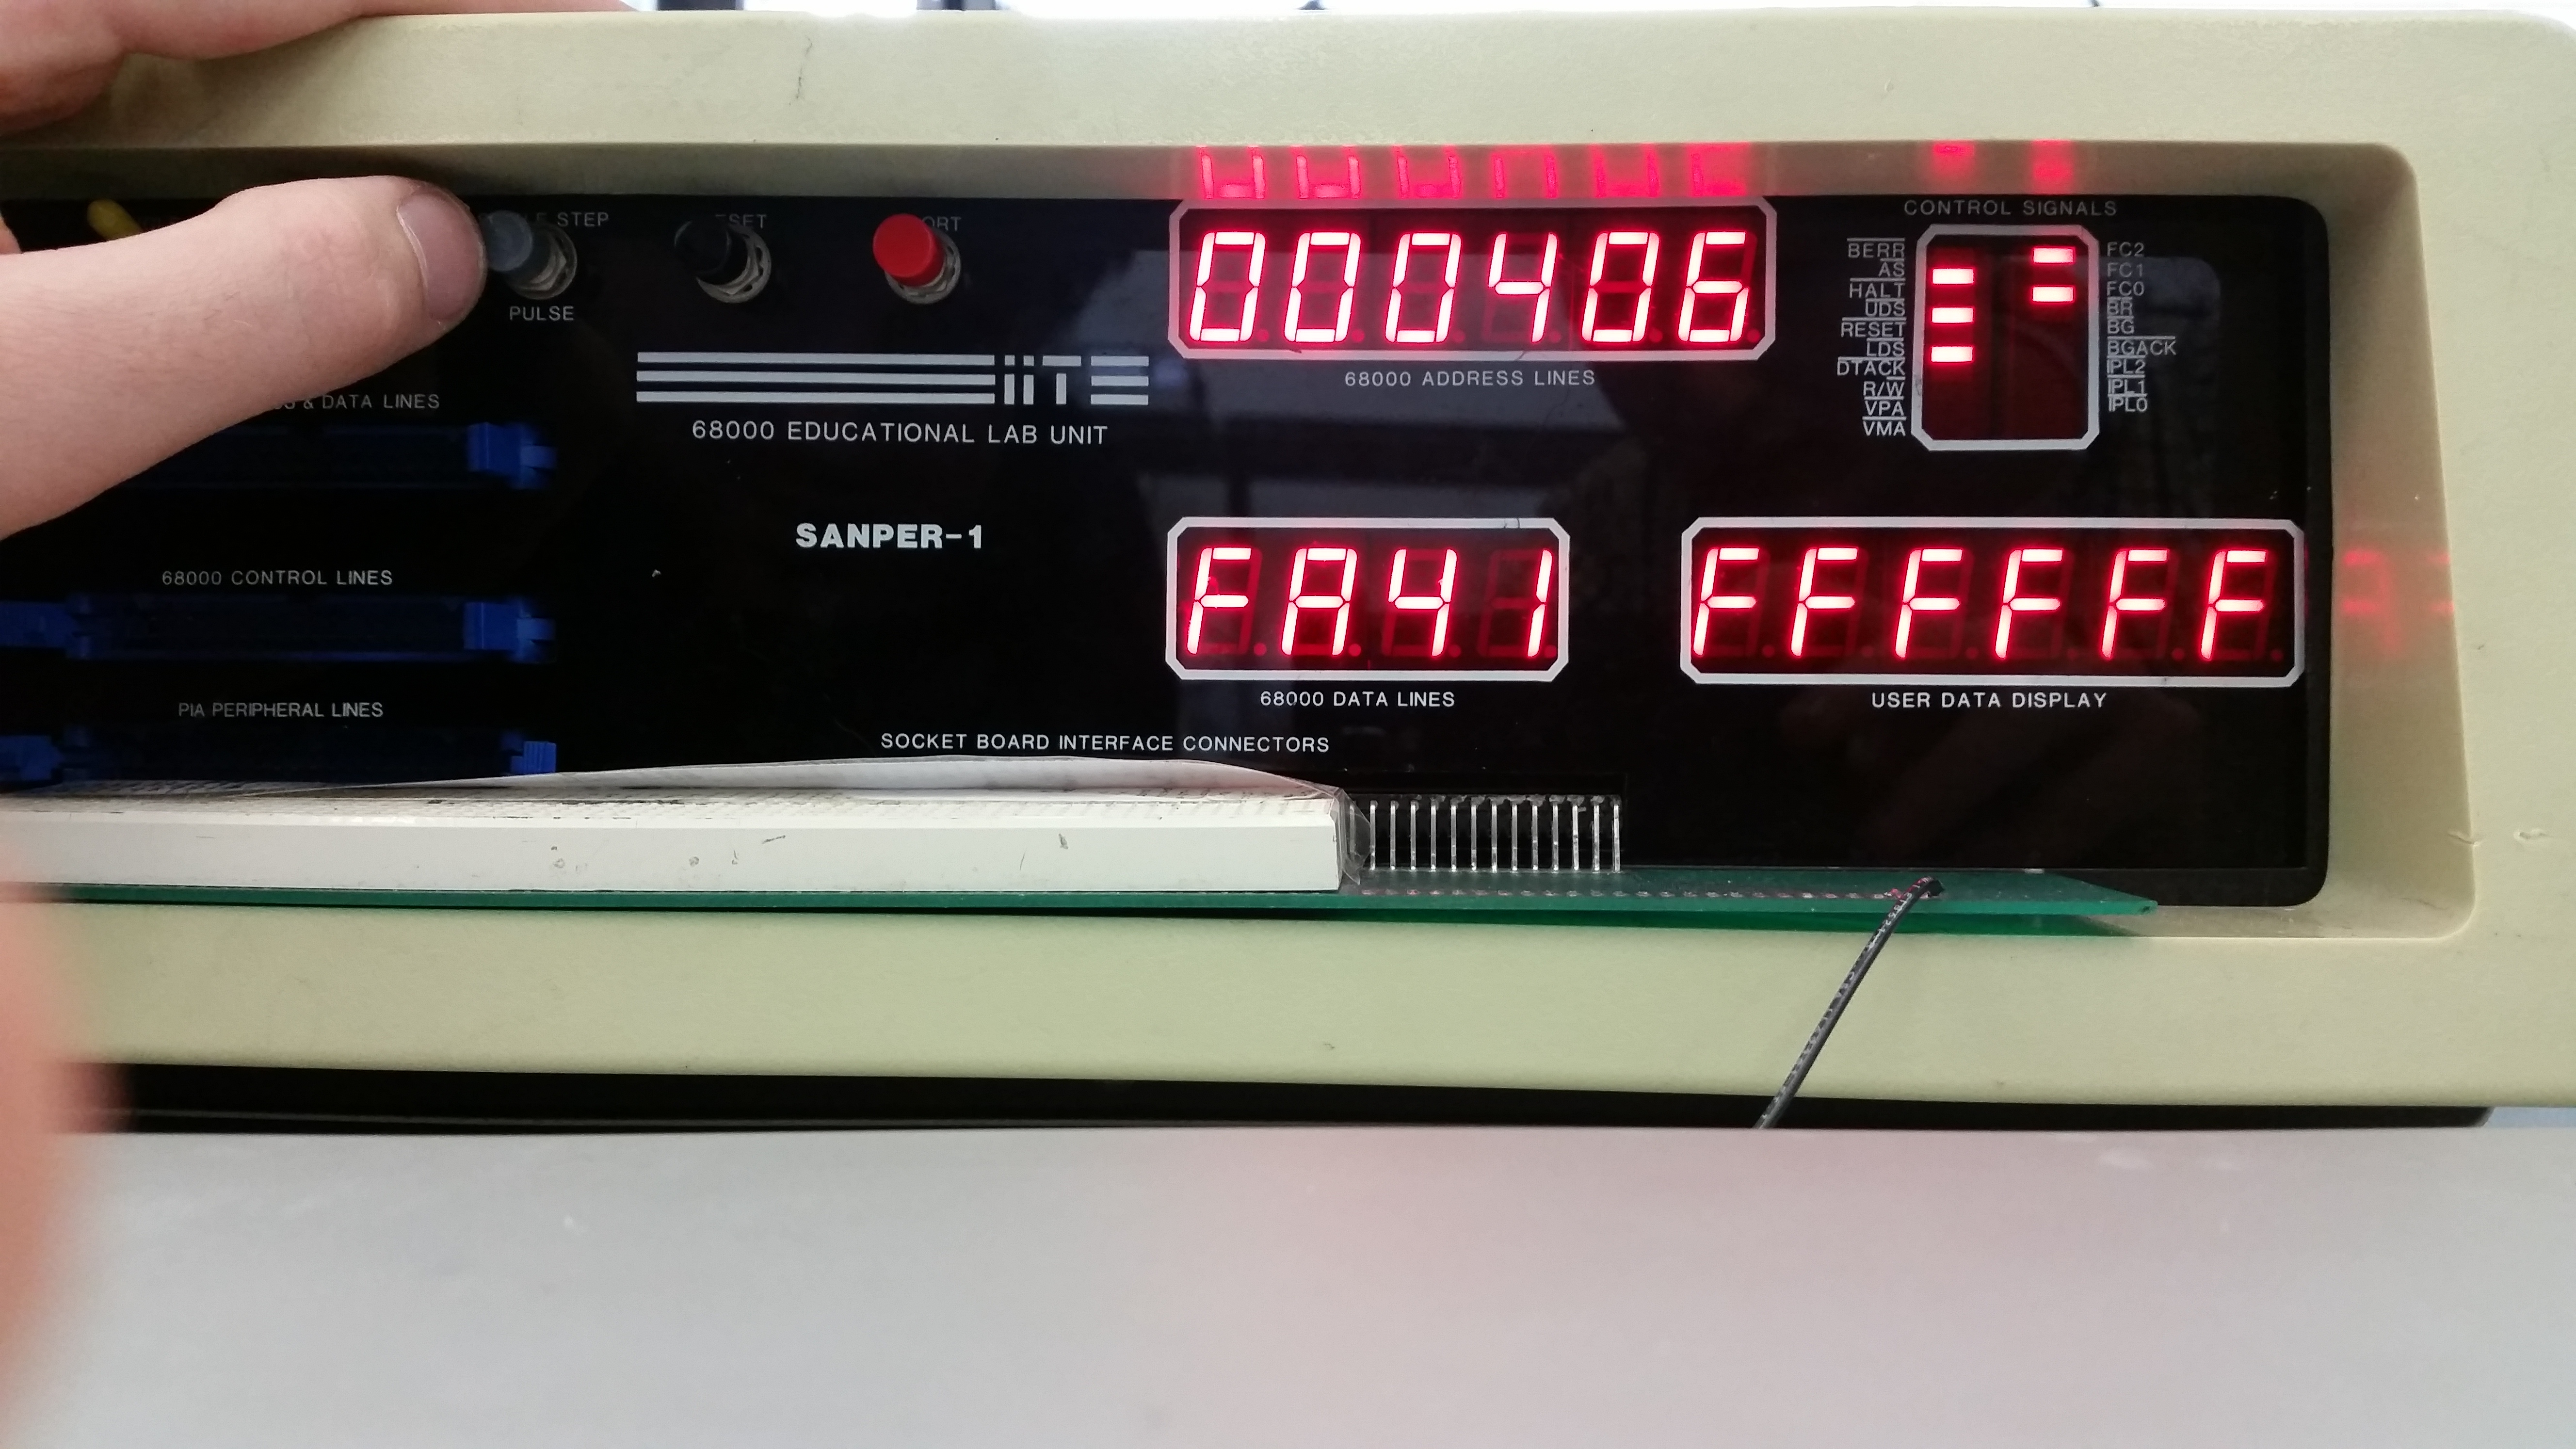
\includegraphics[width=1\linewidth]{Lab1/20150120_095014}
\end{center}
\begin{center}
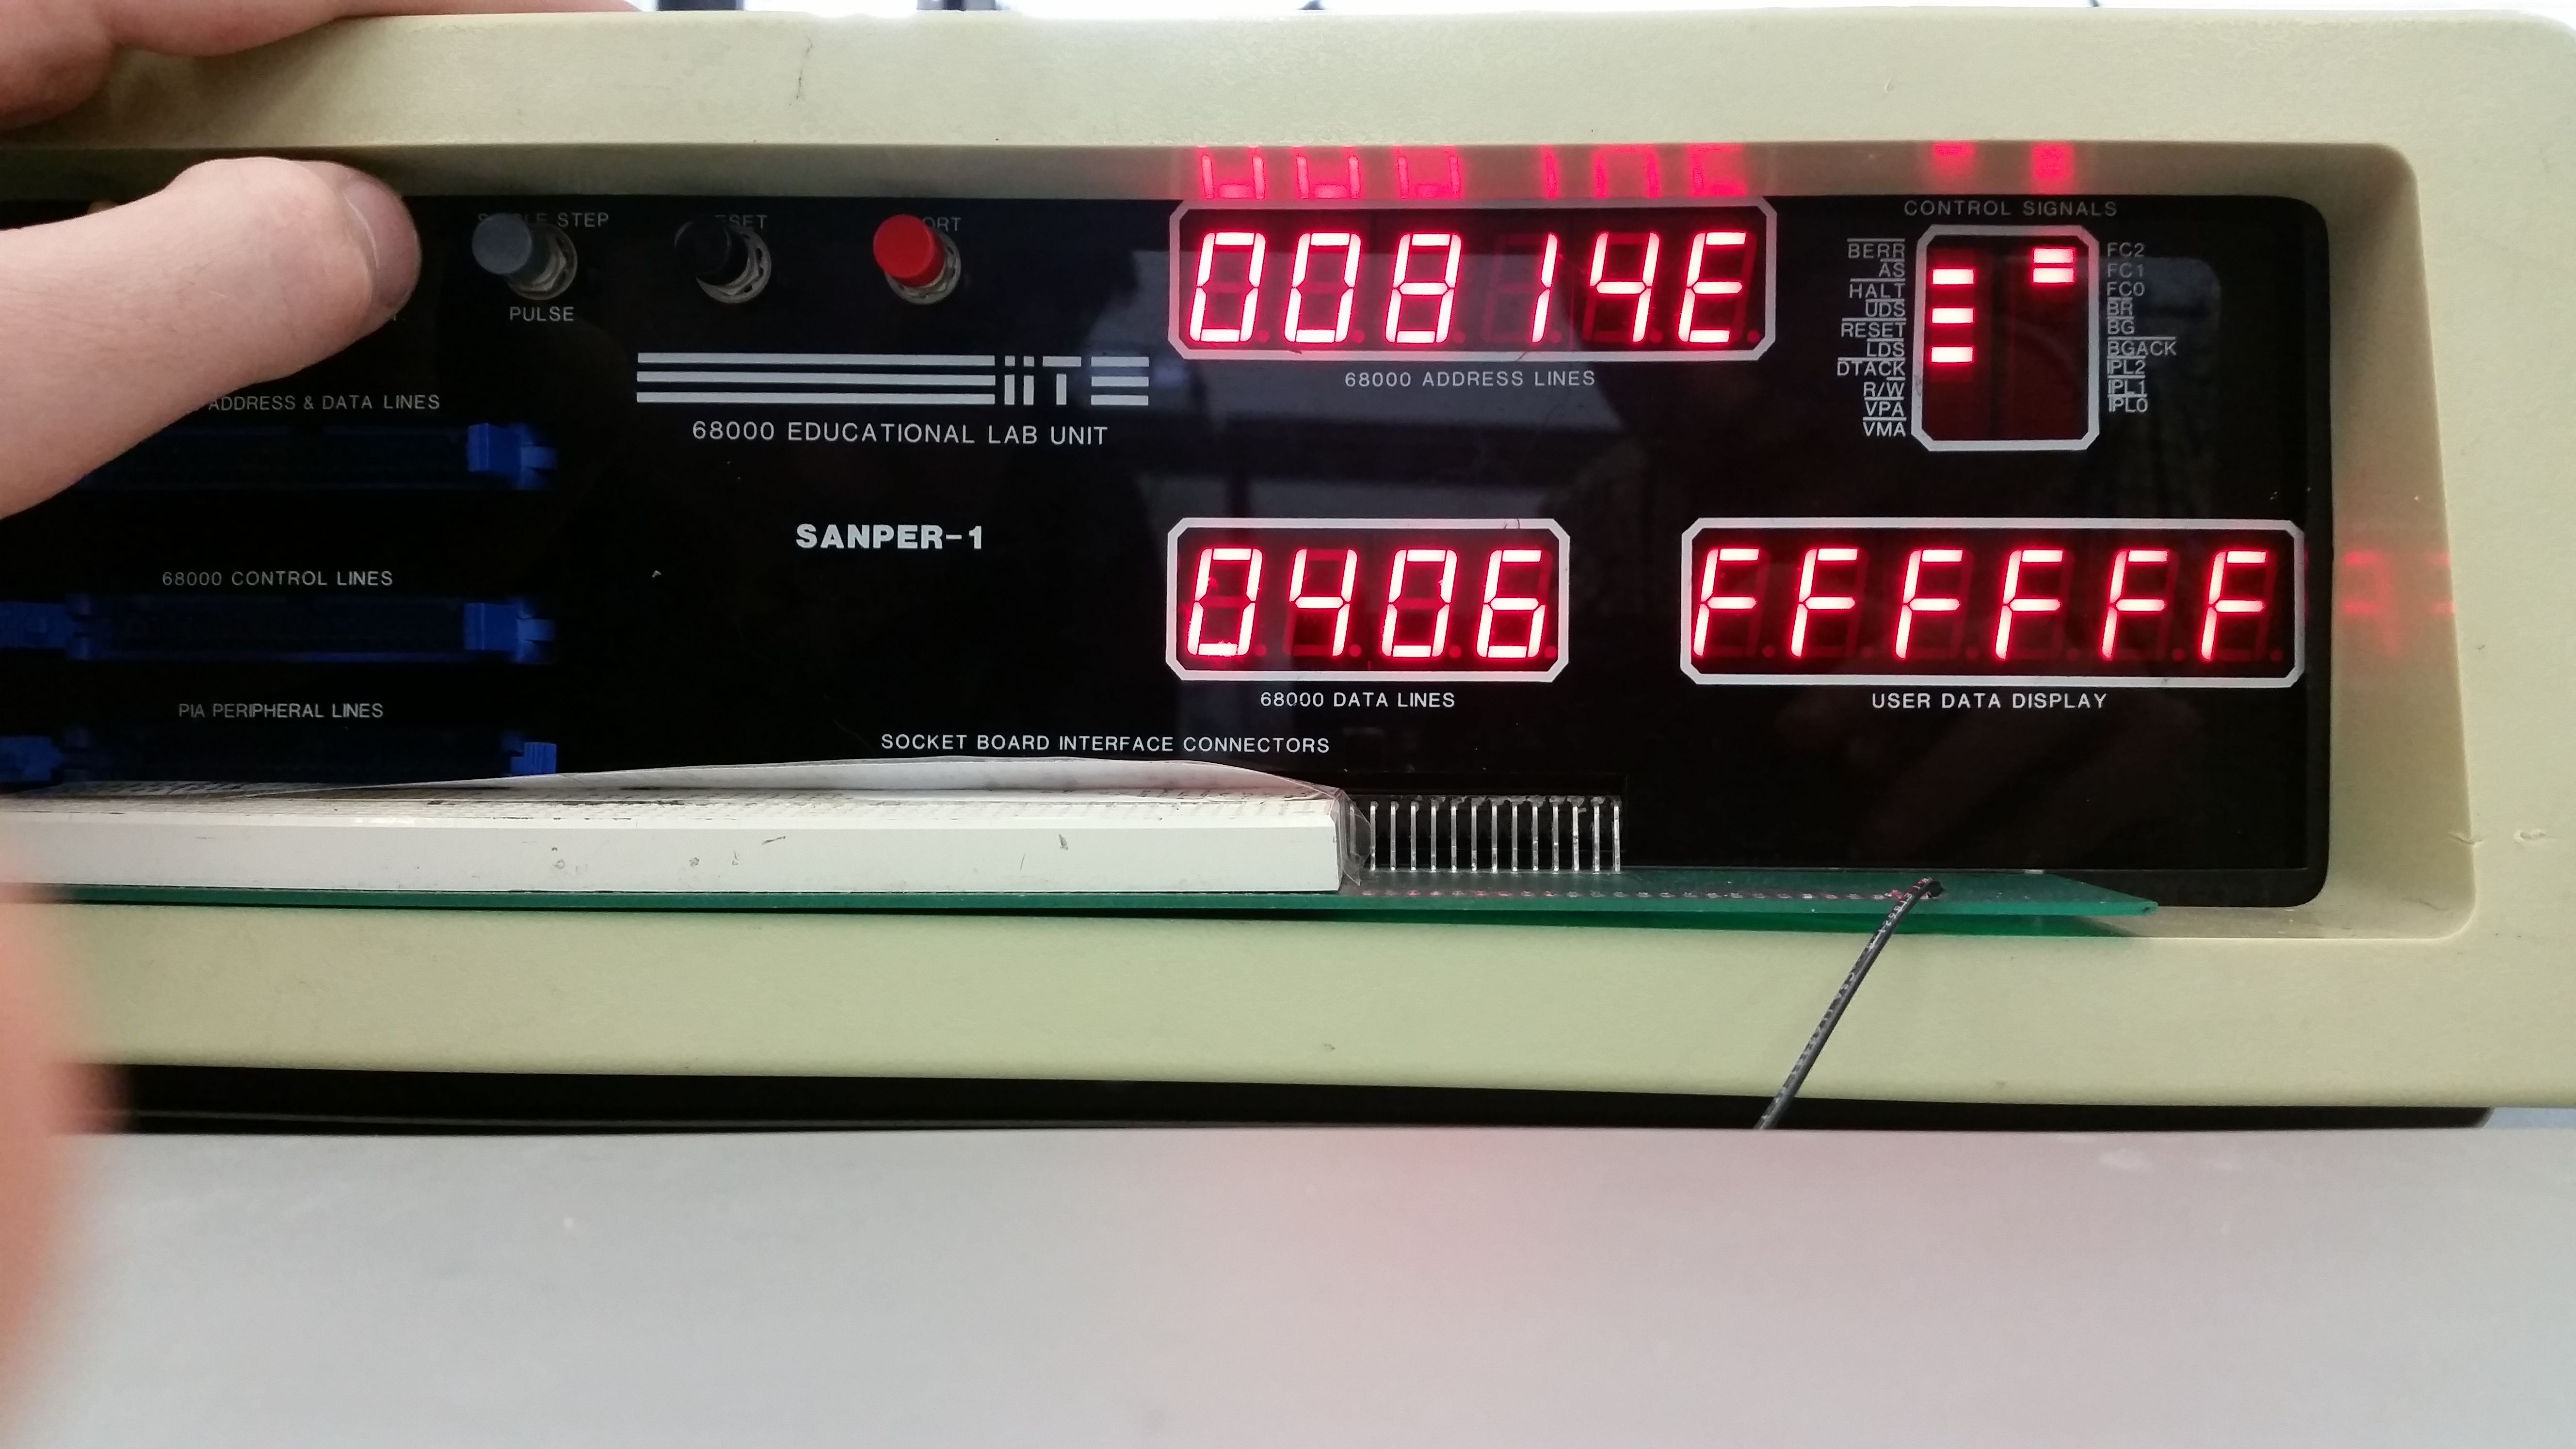
\includegraphics[width=1\linewidth]{Lab1/20150120_095016}
\end{center}
\subsubsection{Software Abort}
\label{abort}
\begin{center}
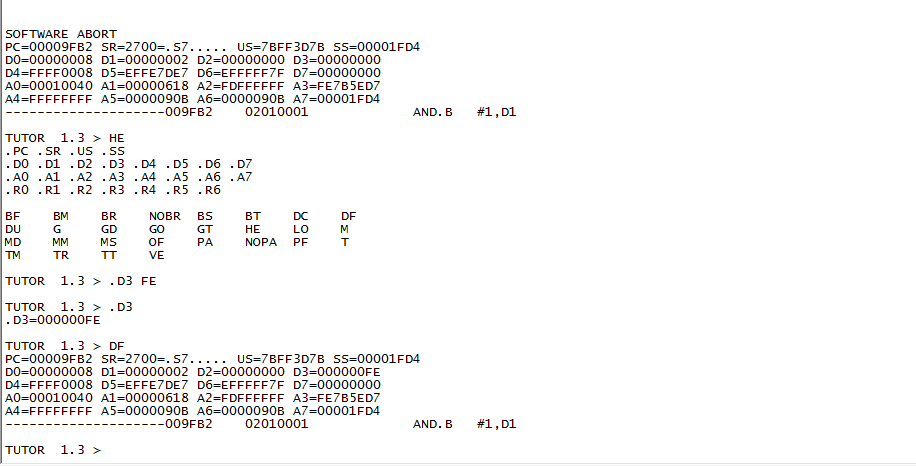
\includegraphics[width=2\linewidth]{Lab1/ABORT1}
\end{center}

\begin{thebibliography}{1}
\bibitem{expman} Experiment 1 Lab Manual
\bibitem{ecbm} Educational Computer Board Manual
\bibitem{m68k}MC68K User Manual
\bibitem{sanper}SANPER-1 ELU User Manual


\end{thebibliography}

\end{document}